%%%%%%%%%%%%%%%%%%%%%%%%%%%%%%%%%%%%%%%%%%%%%%%%%%%%%%%%%%%%%%%%%%%%%%%%%%%%
% AGUtmpl.tex: this template file is for articles formatted with LaTeX2e,
% Modified July 2014
%
% This template includes commands and instructions
% given in the order necessary to produce a final output that will
% satisfy AGU requirements.
%
% PLEASE DO NOT USE YOUR OWN MACROS
% DO NOT USE \newcommand, \renewcommand, or \def.
%
% FOR FIGURES, DO NOT USE \psfrag or \subfigure.
%
%%%%%%%%%%%%%%%%%%%%%%%%%%%%%%%%%%%%%%%%%%%%%%%%%%%%%%%%%%%%%%%%%%%%%%%%%%%%
%
% All questions should be e-mailed to latex@agu.org.
%
%%%%%%%%%%%%%%%%%%%%%%%%%%%%%%%%%%%%%%%%%%%%%%%%%%%%%%%%%%%%%%%%%%%%%%%%%%%%
%
% Step 1: Set the \documentclass
%
% There are two options for article format: two column (default)
% and draft.
%
% PLEASE USE THE DRAFT OPTION TO SUBMIT YOUR PAPERS.
% The draft option produces double spaced output.
%
% Choose the journal abbreviation for the journal you are
% submitting to:

% jgrga JOURNAL OF GEOPHYSICAL RESEARCH
% gbc   GLOBAL BIOCHEMICAL CYCLES
% grl   GEOPHYSICAL RESEARCH LETTERS
% pal   PALEOCEANOGRAPHY
% ras   RADIO SCIENCE
% rog   REVIEWS OF GEOPHYSICS
% tec   TECTONICS
% wrr   WATER RESOURCES RESEARCH
% gc    GEOCHEMISTRY, GEOPHYSICS, GEOSYSTEMS
% sw    SPACE WEATHER
% ms    JAMES
% ef    EARTH'S FUTURE
% ea    EARTH AND SPACE SCIENCE
%
%
%
% (If you are submitting to a journal other than jgrga,
% substitute the initials of the journal for "jgrga" below.)

\documentclass[draft,gc]{agutex}

%%%%%%%%%%%%%%%%%%%%%%%%%%%%%%%%%%%%%%%%%%%%%%%%%%%%%%%%%%%%%%%%%%%%%%%%%%%%
% Self defined usepackage (begin)
%%%%%%%%%%%%%%%%%%%%%%%%%%%%%%%%%%%%%%%%%%%%%%%%%%%%%%%%%%%%%%%%%%%%%%%%%%%%
\usepackage{gensymb} %for ``\degree''
\usepackage[maxfloats=66]{morefloats} %for solving the error: ``! LaTeX Error: Too many unprocessed floats.''
\usepackage{diagbox} % for table cell with a diagonal line and 2 sub cells
%%%%%%%%%%%%%%%%%%%%%%%%%%%%%%%%%%%%%%%%%%%%%%%%%%%%%%%%%%%%%%%%%%%%%%%%%%%%
% Self defined usepackage (end)
%%%%%%%%%%%%%%%%%%%%%%%%%%%%%%%%%%%%%%%%%%%%%%%%%%%%%%%%%%%%%%%%%%%%%%%%%%%%

% To create numbered lines:

% If you don't already have lineno.sty, you can download it from
% http://www.ctan.org/tex-archive/macros/latex/contrib/ednotes/
% (or search the internet for lineno.sty ctan), available at TeX Archive Network (CTAN).
% Take care that you always use the latest version.

% To activate the commands, uncomment \usepackage{lineno}
% and \linenumbers*[1]command, below:

 \usepackage{lineno}
 \linenumbers*[1]
%  To add line numbers to lines with equations:
%  \begin{linenomath*}
%  \begin{equation}
%  \end{equation}
%  \end{linenomath*}
%%%%%%%%%%%%%%%%%%%%%%%%%%%%%%%%%%%%%%%%%%%%%%%%%%%%%%%%%%%%%%%%%%%%%%%%%
% Figures and Tables
%
%
% DO NOT USE \psfrag or \subfigure commands.
%
%
%  Uncomment the following command to include .eps files
%  (comment out this line for draft format):
  \usepackage[dvips]{graphicx}
%
%  Uncomment the following command to allow illustrations to print
%   when using Draft:
  \setkeys{Gin}{draft=false}
%
% Substitute one of the following for [dvips] above
% if you are using a different driver program and want to
% proof your illustrations on your machine:
%
% [xdvi], [dvipdf], [dvipsone], [dviwindo], [emtex], [dviwin],
% [pctexps],  [pctexwin],  [pctexhp],  [pctex32], [truetex], [tcidvi],
% [oztex], [textures]
%
% See how to enter figures and tables at the end of the article, after
% references.
%
%% ------------------------------------------------------------------------ %%
%
%  ENTER PREAMBLE
%
%% ------------------------------------------------------------------------ %%

% Author names in capital letters:
\authorrunninghead{XIAOCHUAN TIAN and EUNSEO CHOI}

% Shorter version of title entered in capital letters:
\titlerunninghead{3D MODELS FOR MID-OCEAN RIDGES}

%Corresponding author mailing address and e-mail address:
\authoraddr{Corresponding author: X. Tian,
Center for Earthquake Research and Information, University of Memphis, 3892 Central Ave., Memphis, TN 38152, USA.
  (xtian@memphis.edu)}

\begin{document}

%% ------------------------------------------------------------------------ %%
%
%  TITLE
%
%% ------------------------------------------------------------------------ %%


\title{3D Numerical Models for Along-axis Variations in Diking at Mid-Ocean Ridges}
%
% e.g., \title{Terrestrial ring current:
% Origin, formation, and decay $\alpha\beta\Gamma\Delta$}
%

%% ------------------------------------------------------------------------ %%
%
%  AUTHORS AND AFFILIATIONS
%
%% ------------------------------------------------------------------------ %%


%Use \author{\altaffilmark{}} and \altaffiltext{}

% \altaffilmark will produce footnote;
% matching \altaffiltext will appear at bottom of page.

\authors{X. Tian,\altaffilmark{1}
Eunseo Choi,\altaffilmark{1}}

\altaffiltext{1}{Center for Earthquake Research and Information, University of
Memphis, 3892 Central Ave., Memphis, TN 38152, USA.}

%\altaffiltext{2}{Department of Geography, Ohio State University,
%Columbus, Ohio, USA.}
%% ------------------------------------------------------------------------ %%
%
%  ABSTRACT
%
%% ------------------------------------------------------------------------ %%

% >> Do NOT include any \begin...\end commands within
% >> the body of the abstract.

\begin{abstract}
Bathymetry reveals diverse morphologies at Mid-ocean Ridges (MORs). Previous studies show that the morphologies at slow spreading MORs are mainly controlled by the ratio (M) between rates of magma supply and plate extension. 2D models successfully explain many cross-sectional observations across the ridge axis. However, magma supply varies along the ridge and the interactions between the tectonics and magmatism at MORs are inevitably three dimensional. We investigate the consequences of this along-axis variations in diking in terms of faulting patterns and the associated structures using a 3D parallel geodynamic modeling code, SNAC. Many observed structural features are reproduced: e.g., abyssal hill, oceanic core complex (OCC), inward fault jump, mass wasting, hourglass-shaped median valley, corrugation and mullion structure. We also propose asynchronous faulting-induced tensile failure as a new possibility for explaining corrugations. $\bar{M} =$ 0.65 is suggested as a boundary value for separating abyssal hills and oceanic core complexes (OCCs) formation. Previous inconsistency in the M range for OCC formation between 2D model results (M $=$ 0.3$\sim$0.5) and field observations (M $<$ 0.3 or M $>$ 0.5) is reconciled by the along-ridge coupling between different faulting regimes.  
\end{abstract}

%% ------------------------------------------------------------------------ %%
%
%  BEGIN ARTICLE
%
%% ------------------------------------------------------------------------ %%

% The body of the article must start with a \begin{article} command
%
% \end{article} must follow the references section, before the figures
%  and tables.

\begin{article}

%% ------------------------------------------------------------------------ %%
%
%  TEXT
%
%% ------------------------------------------------------------------------ %%

\section{Introduction}
\subsection{Review of Literature}
Geodynamic modeling as well as a variety of geological, geophysical observations and lab experiments have provided insight into the processes occurring at the mid-ocean ridges (MORs) \citep[e.g.,][]{Tucholke1994,Blackman2004,Behn2006,Behn2008,Ito2008,Baines2008,Escartin2008,Canales2008,Dick2008,Dannowski2010,Olive2010,Reston2011a,Reston2011b}. In particular, the advent of high-resolution multi-beam bathymetric data has made it possible to discover differences in axial topography between slow and fast spreading ridges and morphological transition from the center of a ridge segment to the tip of the ridge segment.

Variations in morphologies among different MORs are mainly controlled by four factors: magma supply, tectonic strain, hydrothermal circulation and spreading rate \citep{Fowler2004}. Among them, the spreading rate shows the strongest correlation with the ridge morphology. Slow-to-intermediate spreading ridges (half spreading rate less than 4 cm/yr) produce median valleys that are typically 10$\sim$20 km wide and 1$\sim$2 km deep (e.g., Mid-Atlantic Ridges, Figure \ref{fig_Intro1_1}). Fast-spreading ridges (half spreading rate greater than 5 cm/yr) like the East Pacific Rise have axial highs that are 10$\sim$20 km wide, 0.3$\sim$0.5 km high (Figure~\ref{fig_Intro1_3}).

Slow spreading ridges exhibit along-axis variations in off-axis morphology, the width and depth of median valleys and crustal thickness.  Figure~\ref{fig_Intro2_1} shows that the topographic profile near the center of the ridge segment (A-A$^{\prime}$) is rather symmetrical and has a shorter wavelength with a median valley $\sim$12 km wide and $\sim$1 km deep. In constrast, the near-tip profile (B-B$^{\prime}$) is asymmetrical and has a much longer wavelength with a median valley wider than 30 km and shows a greater relief ($\sim$3 km). Gravity data of different ridge segments along MAR (28$\sim$31 $\degree$N and 33$\sim$37 $\degree$N) suggests that the maximum along-axis variation in crustal thickness $\Delta H_{c}$ of a single segment increases with the segment length L \citep{Chen1999} and the relationship is $\Delta H_{c}$(L) = 0.0206L (Figure~\ref{fig_Intro3_1}).

Magma supply at the MORs is mostly a passive process when no hot plume is present \citep{Fowler2004}. Driven by both vertical pressure difference and buoyancy due to horizontal density difference, hot mantle rises up to fill the vacated room produced by the plate separation. Decompression of the upwelling hot mantle results in partial melting. The generated magma upwells to the upper crust and feeds the dikes at the ridge center.

The passive nature of the melting process at the MORs leads to the major difference between fast and slow spreading ridges. At fast spreading ridges, magma is generated at a higher rate than at slow spreading ridges. Thus, fast spreading ridges experience more frequent diking, which efficiently releases stresses generated by far-field forces that drives the plate motion. In contrast, diking is less frequent at slow spreading ridges and can only partially release the stresses associated with plate motion. Thus, the brittle lithosphere of slow-spreading ridges experiences internal deformations (e.g., tectonic processes like normal faulting) when the deviatoric stress exceeds the internal strength of the lithosphere.

\citet{Buck2005} defined the ratio between the rates of dike widening and plate separation as M = $V_{dx}/2V_{x}$, where $V_{dx}$ is the rate of horizontally opening by diking at the ridge center and $V_{x}$ is the half spreading rate of the MOR. According to this definition, M = 1 represents the case where dike injection is so frequent that magma supply is sufficient to release all the tensional stresses from plate separation. M = 0 corresponds to the case of no magma supply, in which diking does not account for any of the plate motion and therefore plates kinematics requires plates to go through internal deformations. As shown in Figure~\ref{fig_Intro5_1}, an axial high forms at a fast spreading ridge (M = 1) due to buoyancy from lateral density difference across ridge axis but a median valley forms at a slow-spreading ridge (M = 0.5) due to near-axis normal faulting, which is in turn caused by the stretching of oceanic lithosphere.

\citet{Tucholke2008} expand the investigation on the role of M in mid-ocean ridge mechanics. They focus on the faulting behaviors of slow spreading ridges and find that the OCCs are most likely to form when M varies from 0.3 to 0.5. When M = 0.7 (Fig.~\ref{fig_Intro6_1}), repeated diking pushes faults that have formed at the spreading center away from the ridge axis. Since the thickness of the brittle layer increases away from the ridge axis due to cooling effects, frictional and bending energy for maintaining the fault also increases. When the energy needed for maintaining an existing fault exceeds the energy for breaking a new near-axis fault, the old fault is replaced by the new one and most of the extension is accommodated by the new fault. When M = 0.3$\sim$0.5, the normal fault remains active for a long time and rotates to a low angle normal fault (detachment fault), exhuming the lower crust and mantle materials to the seafloor. When M $<$ 0.3, most of the tension is accommodated by intra-plate deformations rather than by diking and as a result, faulting pattern is more complicated and unsteady.

\subsection{Statement of Research Purpose}
The M-factor formulation used in the previous 2D models \citep[e.g.,][]{Buck2005,Tucholke2008} successfully explained major features found in across-ridge profiles of seafloor bathymetry. However, 2D models have limitations in studying the along-ridge variations in morphology and faulting patterns. Magma supply at fast spreading ridges seems always sufficient for accommodating plate motions with little variations along the ridge axis. The relatively uniform topography along fast spreading ridges is considered to be consistent with the uniform abundance of the magma supply. However, along the slow spreading ridges, bathymetry, gravity anomaly and results from reflection and refraction seismology show strong correlation with variations in crustal thickness \citep[e.g.,][]{Lin1990, Tolstoy1993, Chen1999, Ryan2009}. Because oceanic crust is mainly formed by upwelling magma at the ridge center, variation in the thickness of the crust implies variation in magma supply. At slow spreading ridges, the degree of cooling by hydrothermal circulation, thermal structures and even local spreading rate \citep{Baines2008} also vary both along and across the ridge axis and they appear interrelated. Thus, for slow-to-intermediate spreading ridges, the interactions between tectonics and magmatism at MORs are inevitably 3D processes and 3D numerical models are desirable for investigating the factors that controls both across- and along-ridge morphology variations.

The purpose of this work is to extend the M-factor formulation originally developed for 2D models to 3D by implementing it into a 3D numerical modeling code SNAC \citep{Choi2008}. By systematically exploring the behaviors of the 3D models and comparing them with observations, we aim to better understand how the along-axis variation in diking at slow-to-intermediate mid-ocean ridges is responsible for the observed morphologies.

\section{Methods}
\subsection{Method of approach}
The numerical modeling code, SNAC (\textbf{S}tGermai\textbf{N} \textbf{A}nalysis of \textbf{C}ontinua), is an explicit Lagrangian finite element code that solves the force and energy balance equations for elasto-visco-plastic materials. Figure~\ref{fig_Methods7_3} shows major components of SNAC.

For each time step, strain and strain rates are updated based on the initial or previous velocity fields under the constraints from boundary conditions. A constitutive model returns updated stresses corresponding to these deformation measures. Internal forces are then calculated from the updated stresses, which is plugged into the momentum balance equation together with the body force term. Then, the damped net force divided by inertial mass yields acceleration at a node point, which is time-integrated to velocity and displacement.

A 3D domain is discretized into hexahedral elements, each of which is in turn divided into two sets of tetrahedra. This symmetric discretization prevents faulting from favoring a specific direction or ``mesh grains''.

Rheology for the oceanic lithosphere is assumed to be elasto-visco-plastic (EVP). When viscosity is high at low temperature, the EVP rheology implemented in SNAC essentially becomes the Mohr-Coulomb plasticity with strain weakening that can create shear bands that behave like faults. Strain softening is realized by cohesion decreasing with increasing amount of permanent (i.e., plastic) strain. We assume this relationship is linear for simplicity. It is sufficient for a full description of such a linear strain weakening to define initial and final values of cohesion and a critical plastic strain at which cohesion becomes the final value. We define the rate of strain weakening as the cohesion difference divided by the critical plastic strain and use it as one of the model parameters. When temperature is high and viscosity is low, the rheology becomes the Maxwell viscoelasticity and can model creeping flow. This property of the EVP model makes it possible to set up a structure with a brittle lithosphere and a ductile asthenosphere through a proper temperature distribution. Rheological parameters are taken from previous studies that use a similar rheology [e.g., \citealp{Buck2005}; \citealp{Tucholke2008}] or from lab experiments \citep[e.g.,][]{Kirby1987}. 

For 3D diking processs, the strain $\Delta\varepsilon_{xx}$ associated with diking leads to stress changes, $\Delta\sigma_{xx}$, $\Delta\sigma_{yy}$ and $\Delta\sigma_{zz}$. These stress changes due to diking are computed according to the linear elastic constitutive equation $\sigma_{ij}=\lambda\varepsilon_{kk}\delta_{ij}+2\mu\varepsilon_{ij}$.

\subsection{Model Setup}
The 3D models have a common geometry of 60 km $\times$ 20 km $\times$ 20 km in $x$, $y$ and $z$ axes respectively with a resolution ($\Delta x$) of 1 km (i.e., $\Delta x$ is the size of each hexahedron element) (Fig.~\ref{fig_Methods8_1}). The initial temperature field linearly increases from 0 \degree C at the top surface to 240 \degree C at the depth of 6 km, reflecting enhanced cooling due to hydrothermal circulation. Below 6 km, the temperature profile follows the instantaneous cooling of a semi-infinite half-space model of moving plates \citep[e.g.,][]{Turcotte2002}. Two sides perpendicular to the $z$ coordinate axis are free-slip. Hydrostatic sea water pressure is added on top of the seafloor. The heights of the water columns are locally determined as (4000 - $h(x,z)$) m, where $h(x,z)$ is the topography at a location, $(x,z)$. The bottom boundary is free of shear stresses and is supported by normal stresses that equal to the local lithostatic pressure (Winkler foundation) following \citet{Buck2005}. Temperature is fixed at 0 \degree C on the top surface and at 1300 \degree C on the bottom surface.

Diking, controlled by the factor M, is assumed to occur in the middle of the doamin (Fig.~\ref{fig_Methods8_1}), where the lithosphere is the thinnest.

We adopt the linear isotropic elasticity, power-law viscosity of dry diabase \citep[e.g.,][]{Kirby1987, Buck2005} and the Mohr-Coulomb plastic model. The complete list of model parameters are given in Table~\ref{Tab_ModelParameters}.

Before running 3D models, we have run hundreds of psedudo-2D models for initial setup and benchmarking with previous studies \citep[e.g.,][]{Buck2005, Tucholke2008}. Preliminary pseudo-2D results show that the model behavior in faulting pattern is sensitive to the rate of strain weakening. Two cases of strain weakening are tested in the 3D models. In one case (denoted as Type 1 weakening), cohesion linearly decreases from 44 MPa (denoted as $C_{i}$) to 4 MPa ($C_{e}$) for plastic strain accumulating from 0 ($\varepsilon_{p_{i}}^{1}$) to 0.1 ($\varepsilon_{p_{e}}^{1}$). It has a characteristic fault slip of 150 m for pseudo-2D models and 300 m for 3D models. The other case (Type 2 weakening) assumes cohesion linearly decreasing from 44 MPa ($C_{i}$) to 4 MPa ($C_{e}$) for plastic strain accumulating from 0 ($\varepsilon_{p_{i}}^{2}$) to 0.33 ($\varepsilon_{p_{e}}^{2}$). In this case, the characteristic fault slip for pseudo-2D models is 500 m and for 3D models is 1 km. The characteristic fault slip is defined as $\Delta X_{c}$=3$\Delta x \varepsilon_{p_{e}}$ where 3 $\Delta x$ represents the thickness of the shear bands which is usually 2 to 4 times $\Delta x$ (size of a hexahedron element) \citep{Lavier2000}. When $\Delta X_{c}$ amount of slip takes place at the fault interface, the cohesion of the material at the faulting interface decreases to $C_{e}$. In this way, under the same amount of $\Delta X_{c}$, models with different resolution should produce the same faulting patterns.

Although how to estimate the M values from observations is a subject of on-going research, constraints are available from a large dataset of bathymetry, gravity and seismic surveys as well as geological drilling. Generally, at slow spreading ridges, magma supply focuses at the center of the ridge segment and decreases towards the tip of the segment \citep[e.g.,][]{Tolstoy1993,Chen1999,Carbotte2015}. There is also evidence for shorter wavelength of 10 to 20 km discrete focus of magma accretion along the ridge axis \citep{Lin1990}.

The numerical cost of a 3D model is non-trivial. For 2 Myr of model time, each model usually runs on 192 cores for about 48 hours (i.e., around 10$^{4}$ core-hours).

Based on the observational constraints and computational cost, we start considering a few scenarios of variations in M along the ridge axis. They are 1) three types of functional forms, linear, sinusoidal and square root; 2) three ranges of M variation along the ridge axis, 0.5 to 0.7, 0.5 to 0.8 and 0.2 to 0.8; and 3) two types of weakening rate, type 1 and type 2.

While 18 models are possible, we could run 15 models with the available computational resources. The complete list of the models is given in Table~\ref{Tab1_1}. 

\section{Results}
\subsection{Reference model}\label{sec_M28LinT1}
We consider the model with M varying linearly from 0.2 to 0.8 along the ridge axis with type 1 weakening rate as the reference model and denote it as M28LinT1 following the shorthand notations given in Table~\ref{Tab1_1}. We describe the general model behaviors in this section and then provide details and mechanisms of the major structural features of the model in the next section.

For the first 7.5 kyr (Figure~\ref{fig_Results1_1}.a), normal faults, represented by localized plastic strain, begin to form near the ridge axis. Because stresses due to plate extension accummulate faster at the lower M side than at the higher M side, faults first initiate at the lower M side and then propagate to the higher M side. Such an asynchronous initiation of faults along the ridge axis creates offset in breakaway at later stages, i.e., the breakaway at the lower M side moves further away from the ridge axis than that of the higher M side (Figure~\ref{fig_Results1_4}).

Likewise, the model produces a median valley that widens and deepens with rates inversely proportional to the M value (i.e., rate of local magma supply) (Fig.~\ref{fig_Results1_1}a-c; Fig.~\ref{fig_Results1_4}a-d).

By 52.5 kyr (Figure~\ref{fig_Results1_1}.b), the normal fault on the right-hand side of the ridge axis remains active while the one on the left becomes inactive. The upper part of the active fault plane (shown as plastic strain in the model) is exposed to the seafloor. As the active fault slips, crust at the footwall bends in a clockwise rotation as is illustrated in Figure~\ref{fig_Results4_8}.

The active normal fault on the right rotates to a lower dip of $\sim$30 $\degree$ at the root of the fault and to $\sim$0 $\degree$ at the exposed fault interface after about 240 kyrs (Fig.~\ref{fig_Results1_1}.c). However, the normal fault at the higher M side (especially for M $>$ 0.7) experiences less fault rotation and the termination of the fault is closer to the ridge axis. The maximum relief between the breakaway and the trough inside the median valley becomes larger than 1 km. In addition, $\sim$2 km wavelength corrugations begin to form between the breakaway and termination at the lower M side (M $<$ 0.35). We discuss the formation mechanism for the corrugations in Discussion.

By 650 kyr (Figure~\ref{fig_Results1_1}.d), the detachment fault reaches its lowest dip angle and its termination stops moving away from the ridge axis. The original breakaway of this detachment has already moved out of the model domain. The total fault offset at this point is greater than the thickness of the crust and thus would be sufficient for exhuming the upper mantle materials.

A new near-axis fault first appears at the center of the model domain with M $\in$ (0.5, 0.65) and then propagates in positive $z$ direction (Fig.~\ref{fig_Results1_1}.d,e). At this time, the initial detachment fault is still active and takes up most of the extension.

The new near-axis normal fault at the higher M side cuts through the hanging wall of the detachment fault at 880 kyr (Fig.~\ref{fig_Results1_1}.f). It coexists with the initial detachment fault and begins to accommodate most of the intra-plate extension. This event is called the ``inward fault jump'' [\citealp{Tucholke1998}; \citealp{Dick2008}].

By 910 kyr (Fig.~\ref{fig_Results1_1}.g), the inward fault jump completes in the M $> 0.5$ region: the new high-angle fault takes up all the extension and the initial detachment fault becomes completely inactive. The block that was previously a hanging wall to the detachment becomes a footwall of the new fault, passively moving with the plate to the negative $x$-axis direction. At the lower M side, the detachment is still active and the hanging wall continues to move toward the positive $x$-axis direction (Figure~\ref{fig_Results_1_velocity_field}). This dextral sense of relative motions between the high and the low M side produces a region of sinistral shear stress $\sigma_{xz}$ (Figure~\ref{fig_Results_1_Sxz}) and eventually creates a transfer fault (Fig.~\ref{fig_Results1_1}.h). As the inward jumped fault evolves, another dome ajacent to the initial OCC is produced at the higher M side by 1000 kyr.

\subsubsection{Constant M model M88ConT2}
As a comparison to the varying M models, a constant M model is run. It shows similar behaviors with corresponding 2D models from the previous studies and does not show along-ridge variations in terms of morphology and faulting.

As shown in Figure~\ref{fig_Results1_3}, model M88ConT2 produces a $\sim$20 km wide and 1$\sim$2 km deep median valley, which is similar to the observation of the Mid-Atlantic Ridge. The width and depth of the median valley is almost constant along the ridge as contrast to the varying M models. The variation of the location of the breakaway and termination along the ridge that is mentioned in the reference model (M28LinT1) does not show up. Because the magma supply is constant along the ridge with M = 0.8, there is no stress perturbation along the ridge. Thus, the normal faults along the ridge initiate at the same time and the slipping rate of the fault is also constant along the ridge axis. The synchronized fault initiation results in no offset between breakaways and the constant sliping rate produces no along ridge axis variation in the position of the termination. In addition, neither corrugations nor mullion structures are generated. Normal faults alternate on each side of the ridge axis with a period of $\sim$10 km of plates extension and produce symmetrical shorter wavelength abyssal hills.

\subsection{Main structural characteristics}
We describe seven structural characteristics of the models: location of the termination, geometry of the trough, inward fault jump, fault alternation, mass wasting, hourglass-shaped median valley and corrugations and mullion structures. Since the details of these features differ among the models, they are useful for delineating and contrasting complicated model behaviors.

\subsubsection{Location of termination}
Location of a fault termination varies along the ridge as indicated by black dashed lines in Figure~\ref{fig_Results1_1} and black arrows in Figure~\ref{fig_Results1_2}. The highest strain rate regions (red) in Figure~\ref{fig_Results1_2} can be interpreted as the active detachment fault interfaces. Compared to the two slices with M $>$ 0.5, the distances between terminations and the ridge axis at the lower M side (M $<=$ 0.5) is larger and the dip angles of the detachment faults are lower. For the ridge region with M $>$ 0.5, the fault root is pushed away from the ridge axis due to excessive diking while the termination is closer to the ridge axis due to lower slipping rate of the fault and the asynchronous initiation of faulting along the ridge. Thus the distance between the termination and the fault root is smaller at the higher M side and the dip angle of the fault is higher. However, among the three slices of M $<=$ 0.5, the distances and the dip angles are similar. This is because one end of the detachment fault roots at the same places along the ridge axis (intersection between the center dike and the brittle-ductile transition), and for the other end, the moving rate of the termination has a maximum value that is restricted by the far field extension rate $V_{x}$. Thus, the bending rates of the detachment faults are similar among the three slices of M $<=$ 0.5.

One thing needs to be noted is that the trough at the higher M side corresponds to the terminations but detached from the terminations at the low M side (M $<$ 0.5) as shown in Figure~\ref{fig_Results1_2}.

\subsubsection{Geometry of trough}

The depressed narrow region that developes in the median valley is termed ``trough''. The reference model showed that its shape in the bird's eye view evolves from a straight line parallel to the ridge axis to a line oblique to the ridge axis (Figure~\ref{fig_Results1_4}.a-d). Initially, the trough along the ridge corresponds to the termination. However, at the lower M side (M $<$ 0.5), as the normal fault rotates to a lower dip, the trough is no longer coincident with the fault termination and is moving slowly to the left because the hanging wall is pulled by the conjugate plate. However, the trough on the higher M side (M $>$ 0.5) is pushed away from the ridge axis \citep{Tucholke2008}. But since the trough cannot bypass the termination, the trough at M = 0.8 is restricted closer to the ridge axis. Together it generates the curved shape of the trough (Figure~\ref{fig_Results1_4}.d).

\subsubsection{Inward fault jump}

The inward fault jump (e.g., Fig.~\ref{fig_Results1_1}.f) occurs in most of the models when the energy for maintaining an old fault becomes larger than breaking a new one near the ridge axis. As shown in Figure~\ref{fig_Results1_2}, at the region with M $>$ 0.5, the existing normal fault is pushed away from the ridge-axis due to robust diking (M $>$ 0.5). As it moves away from the ridge axis, the frictional energy for the fault, the bending energy for the footwall as well as the negative work done by gravity that resists the exhumation of the footwall increase [\citealp{Lavier2000, Olive2014}]. The initial detachment fault remains active until the sum of the negative works reaches an upper limit that breaking a new fault near the ridge axis needs less work than to maintain the initial one, the initial detachment fault at the higher M side is then substituted by the inward jumping fault that cuts through the previous hanging wall. As the fault evolves, it connects to the initial detachment at the lower M side (M $<$ 0.5) by a transfer fault and generates a curved termination along the ridge. Unlike fault alternation described below, the inward fault jump occurs on the same side of the ridge axis with its along-axis extent corresponding to the M $>$ 0.5 region.

\subsubsection{Fault alternation}

Fault alternation is the behavior that normal faults alternatively show up on each side of the ridge axis when magma supply is robust enough, as shown in M88ConT2 (Figure~\ref{fig_Results1_3}). The normal fault first evolves on the left-hand side of the ridge axis and produces an abyssal hill parallel to the ridge axis. By 480 kyr, another normal fault evolves on the other side of the ridge axis and replaces the first one. Note that among the 15 models (Table~\ref{Tab1_1}), only three produce fault alternation. They are M88ConT2, M58SinT2 and M58SqrtT2. Fault alternates only when weakening rate is low (type 2 weakening) and the average integration of M along the ridge is large enough. Analysis on when and why fault alternates is given in the Discussion section.

\subsubsection{Mass wasting}\label{para_CutBack}
Mass wasting occurs on the exposed surface of a low-angle normal fault. When the weak fault zone becomes gravitationally unstable and is decoupled from the spreading plate as well as the underlying material, the detached layer flows towards the lower ridge axis and the lower M side driven by gravity with a velocity hundreds of times faster than the half spreading rate (Figure~\ref{fig_Results_3_2_5_Cut-back_velocity}; Figure~\ref{fig_Results4_4}.b,e (first row)). As the top layer of the hanging wall flows down the topography slope, obvious topography drop is observed in 2.5 kyr (Figure~\ref{fig_Results4_4}.b versus c; d versus e (topography)).

Mass wasting is triggered by several factors. First, when the tip of the weak fault interface moves away from the ridge axis with the spreading plate and is intersected by a pre-exisitng shear stress $\sigma_{xy}$ (Figure~\ref{fig_Results4_5}), the extra shear stress cuts the tip of the weak fault interface and leads to the decoupling between the breakaway and the upper layer of the hanging wall of the detachment fault. Second, during the roll over of the hanging wall at the breakaway, tensional stress ($\sigma_{xx} >$ 0) promotes the deviatoric stress for generating small scale high angle normal faults cutting the detachment fault surface \citep{Tucholke1998} (Figure~\ref{fig_Discussion_Observation_1_Tucholke1998}.c,d) and in this case the tip of the weak layer. In addition, along ridge coupling tends to resist the increase in along ridge offset of breakway which is generated by along ridge varying slip rates of the faults. As Figure~\ref{fig_Results_3_2_5_sqrt_cut_back_Sxz_beneath} shows, the dextral sense shear stresses (red $\sigma_{xz}$) beneath the top weak layer tends to rotate the upper layer and assists in triggering the decoupling process.

\subsubsection{Hourglass-shaped median valley}
All the models with M variation develop an hourglass-shaped median valley although the geometry of the median valley changes with time and with the functional forms and ranges of M variation. A median valley of the M28Sqrt model initially has a uniform width along the ridge but is deeper on the lower M side where normal faults first form (Figure~\ref{fig_Results_3_2_hourglass_evolution}.a). By $\sim$100 kyr, the fault on right hand side of the ridge axis does not propagate to the higher M side of the ridge and becomes inactive (Figure~\ref{fig_Results_3_2_hourglass_evolution}.b). It produces a depressed topography curve following the inactive fault trace, which is further away from the ridge axis at the lower M side but closer to ridge axis at the higher M side. On the other side of the ridge axis, as the active fault rotates to a lower dip angle, breakaways at the lower M side move further away from the ridge axis than the breakaways at the higher M side. This along-ridge variation in the location of the breakaways act as another boundary of the hourglass on the left.

By $\sim$170 kyr (Figure~\ref{fig_Results_3_2_hourglass_evolution}.c), the hourglass-shaped median valley continues to widen and deepen. Since the area of the cross section along the ridge inside the hourglass-shaped median valley is approximately inversely proportional to the local M values, the shape of the hourglass varies with different ranges and functional forms of M variations.

In addition, the further depression inside the median valley is mostly due to the elastic deformation from crustal extension. As shown in Figure~\ref{fig_Results4_7}, the $\sigma_{xx}$ in the median valley is higher because the brittle crust is thinner, when same amount of force propagates from far field extension to the median valley, the stress increases. This increased $\sigma_{xx}$ is responsible for the further depression and extension of the median valley on the side of the ridge axis with no active faulting (Figure~\ref{fig_Results_3_2_hourglass_evolution}.d). For the median valley on the other side of the ridge axis, mass wasting between the breakaways and the ridge axis results in further lowering of topography (Figure~\ref{fig_Results4_4}.d versus e (topography)). 

\subsubsection{Corrugations and mullion structures}
Both corrugations and mullion structures are linear structures parallel to the spreading direction. As shown in Figure~\ref{fig_Results1_1}.f, at the M $<$ 0.5 area on top of the OCC surface, corrugations show a uniform wavelength of $\sim$2 km with hundreds of meters in amplitude. At the higher M side of the ridge (Figure~\ref{fig_Results1_1}.g), a mullion structure with a wavelength of $\sim$7 km shows up on the surface of the OCC. In spite of morphological similarity, corrugations and mullion structures have different formation mechanisms.

\paragraph{Corrugations}
The corrugation starts at the breakaway as a response to tensile stress in the $z$-axis direction. As shown in Figure~\ref{fig_Results_3_2_6_corrugations_evolution}, when the plastic strain reaches or excedes 0.1 (red color), on the basis of type 1 weakening, the cohesion decreases to 4 MPa. With a 30 $\degree$ friction angle, tensile failure is declared when the $\sigma_{zz}$ reaches $\sim$7 MPa (yellow color).

The tensile stress is generated by the asynchronous faulting along the ridge. Faulting initiates earlier at the lower M side of the ridge. As the fault offsets more on the lower M side than on the higher M side, the footwall of the fault rotates and get uplifted more on the lower M side. This relative displacement between the footwalls along the ridge generates the isochron-parallel tensional stress $\sigma_{zz}$. Since $\sigma_{zz}$ follows along the moving tip of the plastic strain, the plastic srain together with $\sigma_{zz}$ generate tensile failure that propagates away from the ridge axis and thus produces the linear corrugations that are parallel to the spreading velocity. Detailed analysis along with simpler model experiments are given in the ``Discussion'' section.

\paragraph{Mullion structures}
Mullion structures observed in the models are formed by the along-ridge variation in the location of the termination due to the evolution of faulting. They usually appear where the termination is closer to the ridge axis. The shape of the footwall follows the trace of the termination as it is exhumed to the surface. Where the termination is bent inward to the ridge axis, an ``initial dome'' (Figure~\ref{fig_Results_3_2_6_mullion_evolution}.a) is produced once the footwall is exhumed to the seafloor. The wavelength of the mullion structure is determined by the shape of the termination. If the pattern of the termination lasts for a long time and the footwall of the detachment fault keeps being exhumed to the surface following the trace of the detachment fault termination, a mullion structure is produced (Figure~\ref{fig_Results_3_2_6_mullion_evolution}.b).

\subsection{Effects of the functional forms of M variation}
\subsubsection{M28T1}
Major differences among M28LinT1, M28SinT1 and M28SqrtT1 lie in the model behaviors in terms of the inward fault jump, the mass wasting and the hourglass-shaped median valley. None of the three models show fault alternation. Figure~\ref{fig_Results3_1} shows M variations of three kinds of functional forms.

\paragraph{Inward fault jump}\label{para_InwardFaultJump}
Only the linear (M28LinT1) and sinusoidal (M28SinT1) models have inward fault jump. Sqaure root model (M28Sqrt) does not have inward fault jump because during mass wasting, termination of the detachment fault retreats backward toward the ridge axis and the detachment fault is maintained near the ridge axis.

Comparing linear and sinusoidal models, timing and dimension of the inward jumping faults are different. For the linear functional form, the inward fault jump at the higher M side starts accommodating most of the extension at $\sim$900 kyr and replaces the initial detachment fault (Figure~\ref{fig_Results4_2}, Figure~\ref{fig_Results1_1}.f). It nucleates from the ridge center where M $=$ 0.5 and then propagates to the M $=$ 0.8 end with a length of $\sim$11 km. For the sinusoidal functional form, the inward fault jump takes the place of the initial detachment fault earlier at $\sim$550 kyr with a length of 14 km (Figure~\ref{fig_Results4_2}).

The timing difference between the linear and sinusoidal models is because M28SinT1 consistently has a higher M value than the M28LinT1 (Figure~\ref{fig_Results3_1}), which results in the initial detachment fault at the higher M side (M $>$ 0.5) of M28SinT1 being pushed off axis faster than M28LinT1 and thus forming an earlier inward fault jump. The length difference is because M28SinT1 has a greater length along the ridge axis of M $\ge$ 0.5 (Figure~\ref{fig_Results3_1}).

\paragraph{Mass wasting}

Mass wasting only happens in the M28SqrtT1 model. Qualitatively, it is because M28Sqrt has a much higher value of $\frac{\partial M}{\partial Z}$ at the lower M side (Figure~\ref{fig_Results_3_3_1_M_type_plot_dM_dZ}), which implies a larger along ridge shear stress $\sigma_{xz}$ as well as a larger difference in $\sigma_{xy}$ along the ridge that result in the decoupling between the higher and lower M sides hanging walls.

\paragraph{Hourglass-shaped median valley}
As shown in Figure~\ref{fig_Results_3_3_1_hourglass}, differences among the three models are identified. At 160 kyr, median valley for M28SinT1 has the smallest cross-sectional ($x$-$y$) area at the higher M side (center of the ridge segment). Whereas at the lower M side,  M28SqrtT1 has the smallest cross section. This is because the cross section inside the median valley is inversely proportional to the local M value along the ridge. Moreover, the breakaways at the lower M sides for M28LinT1 and M28SinT1 bend to parallel to the ridge axis while the breakaway for M28SqrtT1 moves further away from the ridge axis. In addition, M28SinT1 has a trough inside the median valley with the highest curvature. At 500 kyr, M28SinT1 has the narrowest median valley at the higher M side and the high topography zone on the left-hand side of the ridge axis is the widest in the $z$-axis direction. Integrating the topography below initial elevation (0 km) inside the median valleys of the three models, M28Sin has the lowest value of integration because it has the largest amount of magma supply of M $>$ 0.5 (Figure~\ref{fig_Results3_1}). In addition, the termination of the detachment fault of M28SqrtT1 has the highest curvature at the lower M sides. All these model behaviors correspond to the M variation (Figure~\ref{fig_Results3_1}).

\subsubsection{M58T2}
Among M58LinT2, M58SinT2 and M58SqrtT2, the major difference lies in ``fault alternation''. Except for the constant M model M88ContT2, among all the models, only the models with type 2 weakening and M ranges from 0.5 to 0.8 (M58) have fault alternation. However, M58LinT2 does not produces alternating fault during the 1.1 Myr model time. Instead, one detachment fault lasts until $\sim$300 kyr when the inward fault jump happens at the higher M side (0.65 $<$ M $<$ 0.8) and replaces the initial detachment fault. This provides a lower limit of $\bar{M}$ that prevents fault alternation and alows a long-lived detachment fault to produce an OCC. As shown in Table~\ref{Tab_3_3_average_M}, the lower limit is 0.6425 for M58LinT2. Detailed analysis of the fault alternation is given in ``Discussion''.

\subsection{Effects of the weakening rate}
\subsubsection{M57SinT1 versus M57SinT2}
Initially, both models develop normal faults on both sides of the ridge axis at the lower M side. In the model with the faster weakening rate (M57SinT1), faults propagate toward the higher M side and cut through the whole crust by 25 kyr but this process completes 25 kyr later in the model with slower weakening rate (M57SinT2). By $\sim$310 kyr, the inward fault jump appears at the higher M side (M $>$ 0.5908) of M57SinT2 whereas at M $<=$ 0.5908, the initial fault remains active (Figure~\ref{fig_Results_Weakenging_2}.c and d). However, when the weakening is fast (M57SinT1), mass wasting happens at $\sim$260 kyr and helps to maintain a relatively higher angle fault with a termination closer to the ridge axis. The initial fault remains and no inward fault jump forms (Figure~\ref{fig_Results_Weakenging_2}.a and b). In addition, the width of median valley at the lower M side is wider for M57SinT2 than M57SinT1 (Figure~\ref{fig_Results_Weakenging_2}.c, d versus a, b) because slower weakening (type 2) alows a more distributed tensional stress $\sigma_{xx}$ rather than fast weakening that once a fault establishes, larger amount of the tensional stress $\sigma_{xx}$ is released at the fault. The amplitude of the corrugations of M57SinT1 is larger than that of slower weakening M57SinT2. This is because faster weakening rate allows a faster decrease in the cohesion. As the cohesion reaches its minimum of 4 MPa ealier when the plastic strain accummulates to 0.1, tensile failure is easy to happen in the isochron parallel direction and produces the corrugations.

\paragraph{M57SinT1}\label{para_M57SinT1}
For M57SinT1, by 400 kyr (Figure~\ref{fig_Results_Weakenging_3}.a), two antithetic faults form at the lower M side (0.5 $<$ M $<$ 0.6521) accommodating part of the plate extension. This makes the termination at the lower M side retreat backward to the ridge axis. By 530 kyr, the termination at the center of the ridge segment (M $=$ 0.6299$\sim$0.6618) moves further away from the ridge axis (Figure~\ref{fig_Results_Weakenging_3}.b). This curved termination leads to a curved topography aligning with it (white curve in the second row). By 740 kyr, another antithetic fault forms at the lower M side (Figure~\ref{fig_Results_Weakenging_3}.c). It doesn't take the place of initial fault and disappear soon, however, it again releases tensional stress and helps maintain a closer to ridge axis termination at the lower M side. By 1000 kyr (Figure~\ref{fig_Results_Weakenging_3}.d), an Atlantiss Massif shape OCC is produced (lower M side has a larger dome and higher M side has a smaller dome due to the along ridge termination evolution. Corrugations with wavelength varying from hundreds meters to kilometers are also produced.

\paragraph{M57SinT2}\label{para_M57SinT2}
For M57SinT2, instead of maintaining a detachment fault like M57SinT1, it produces inward fault jump at the higher M side. By 325 kyr (Figure~\ref{fig_Results_Weakenging_4}.a), an inward fault jump happens and takes the place of the initial detachment fault at the higher M side. Between 447.5 kyr (Figure~\ref{fig_Results_Weakenging_4}.b) and 450 kyr (Figure~\ref{fig_Results_Weakenging_4}.c), a small scale mass wasting happens and the termination recedes backward to the ridge axis. By 600 kyr, the termination at the higher M side extends further (Figure~\ref{fig_Results_Weakenging_4}.d). By 885 kyr, an inward fault jump happens at the higher M side (0.62 $<$ M $<$ 0.7) (Figure~\ref{fig_Results_Weakenging_4}.e). The width of the median valley at the lower M side keeps increasing due to the distributed $\sigma_{xx}$ (Figure~\ref{fig_Results_Weakenging_4}.a$\sim$d).

\subsubsection{M58SinT1 versus M58SinT2}
A major difference between M58SinT1 and M58SinT2 is that only M58SinT2 has fault alternation.
\paragraph{M58SinT1}\label{para_M58SinT1}
During the 1 Myr extension of the model M58SinT1, 10 phases of the evolution of faulting are identified (Figure~\ref{fig_Results_Weakenging_5}.a$\sim$j). Antithetic faults, inward fault jumps, mass wasting happens with a rider block, corrugations and mullion structures produced.

By 240 kyr (Figure~\ref{fig_Results_Weakenging_5}.a), due to fast weakening (type 1), cohesion along the termination is low. Stress $\sigma_{zz}$ takes the advantage and generates $\sim$2 km wavelength corrugations parallel to the spreading direction as the termination moves further away from the ridge axis. Between 240 kyr (Figure~\ref{fig_Results_Weakenging_5}.a) and 245 kyr (Figure~\ref{fig_Results_Weakenging_5}.b), a mass wasting happens at the lower M side. The termination recedes toward the ridge axis during the mass wasting. By 345 kyr (Figure~\ref{fig_Results_Weakenging_5}.c), an antithetic fault forms at the lower M side (0.5 $<$ M $<$ 0.5469) with an inward fault jump happening at ridge segment with M $\in$ (0.5927, 0.6763) (Figure~\ref{fig_Results_3_4_2_3D_Antithetic_fault}). 45 kyr later, the two weak zones break through and connect to each other and take the place of the initial detachment fault at the lower M side (Figure~\ref{fig_Results_Weakenging_5}.d). Due to this inward fault jump, a sinistral $\sigma_{xz}$ zone (blue area in the $\sigma_{xz}$ panel) forms and is bounded by the termination of the inward fault jump near the ridge axis at the lower M side and the termination of the initial detachment fault at the higher M side. By 530 kyr (Figure~\ref{fig_Results_Weakenging_5}.e), the termination of the inward fault jump at the lower M side evolves to a curve with its center moving further away from the ridge axis because the inward fault jump initiates at the center and the new fault starts slipping earlier. However, the lower M side of the curve remains closer to the ridge axis due to the antithetic fault and the other end of the curve is also closer to the ridge axis because the fault initiates later. This curved termination at the lower M side also connects to the initial detachment fault at the higher M side which is further away from the ridge axis. Together, the curved termination is like a mirror reflected letter ``S''. This flipped ``S'' shape termination is also shown in topography. As the curved termination at the higher M side lasts for $\sim$300 kyr since $\sim$390 kyr, following the shape, a $\sim$10 km in wavelength and $\sim$7 km in along spreading direcion mullion structure is formed (Figure~\ref{fig_Results_3_4_2_M58SinT1_mullion_riderBlock_inwardFaultJump}). By $\sim$680 kyr, an inward fault jump hapens at the higher M side (0.7853 $<$ M $<$ 0.7991). It perturbs the curved shape termination and ceases the further exhumation of the mullion structure. This inward fault jump also produces a rider block that covers the inactive detachment fault and moves off axis following the exhuming footwall of the inward jumped fault.

Between 530 kyr (Figure~\ref{fig_Results_Weakenging_5}.e) and 550 kyr (Figure~\ref{fig_Results_Weakenging_5}.f), another mass wasting happens at the lower M side (0.5 $<$ M $<$ 0.5469) where a slump block with a surface area of $\sim$9 km$^{2}$ flows down the topography slope into the trough. Termination recedes backward to the ridge axis. By 580 kyr, termination at the lower M side moves further away from the ridge axis due to less magma supply. Between 580 kyr and 850 kyr, due to two antithetic faults at the lower M side (M $\in$ (0.5, 0.5469) $\cup$ (0.5927, 0.6567)), the termination at the lower M side recedes and the previous mirror reflected ``S'' shape termination evolves to a half circle curve (Figure~\ref{fig_Results_Weakenging_5}.h). The shape is also reflected in the topography. By 960 kyr (Figure~\ref{fig_Results_Weakenging_5}.i)), at the ridge segment with M $\in$ (0.6763, 0.7121), another inward fault jump replaces the detachment fault away from the ridge axis and retreats the termination backward to the ridge axis forming two half circle curves with wavelengths of around half of the model domain in $z$-axis. A large dextral shear zone (red region $\sim$40 $\degree$ oblique to ridge axis) is seen in the $\sigma_{xz}$ panel. The shear stress $\sigma_{xz}$ is produced by the inward fault jump at the center of the ridge segment that previous hanging wall changes to the footwall of the inward jumped fault and generates an offset between the old hangingwall at the lower M end and the new footwall of the inward jumped fault. By 1000 kyr, due to the along ridge coupling, the inward fault jump propogates to the end of the high M side (Figure~\ref{fig_Results_Weakenging_5}.j). 

\paragraph{M58SinT2}\label{para_M58SinT2}
As shown in Figure~\ref{fig_Results_Weakenging_6}, a fault initiates on the left-hand side of the ridge axis (Figure~\ref{fig_Results_Weakenging_6}.a). The breakaway at the lower M side moves away from the ridge axis further than that of the higher M side. It takes longer time of $\sim$100 kyr to form a localized fault plane through the whole ridge segment due to the slower rate of weakening (type 2). By 215 kyr (Figure~\ref{fig_Results_Weakenging_6}.b), fault alternates to the conjugate plate and gradually replaces the initial one. Corrugations are only produced at the lower M side (M $\in$ (0.5, 0.6763)). By 330 kyr, fault alternates again. Between 490 kyr (Figure~\ref{fig_Results_Weakenging_6}.d) and 495 kyr (Figure~\ref{fig_Results_Weakenging_6}.e), a mass wasting happens with termination receding. A slump block with an area of $\sim$16 km$^{2}$ flows down the topography slope into the trough. With fault alternation, the shape of the median valley is no longer a typical hourglass. However, at the lower M side, the median valley is still wider and deeper. Smaller wavelength abyssal hills are produced at the higher M side. 

\subsubsection{M58SqrtT1 versus M58SqrtT2}
The major difference between M58SqrtT1 and M58SqrtT2 is also whether the normal fault alternates or not.
\paragraph{M58SqrtT1}\label{para_M58SqrtT1}
By 260 kyr, breakaway at M $=$ 0.5 moves $\sim$5 km further away from the ridge axis than that at the higher M end (Figure~\ref{fig_Results_Weakenging_7}.a). Corrugations with a wavelength of $\sim$2 km are produced along the ridge. By 370 kyr (Figure~\ref{fig_Results_Weakenging_7}.b), due to larger value of $\frac{\partial M}{\partial Z}$ at the lower M side, a vertical tensile failure takes place at M $\in$ (0.5, 0.5949). Two parallel sinistral shear stress zones (blue) are seen in the $\sigma_{xz}$ panel. By 400 kyr (Figure~\ref{fig_Results_Weakenging_7}.c), an inward fault jump happens where M $\in$ (0.5949, 0.7121) and it propagates to the end of the higher M side and replaces the initial detachment fault at the higher M side by 460 kyr (Figure~\ref{fig_Results_Weakenging_7}.d). By 590 kyr (Figure~\ref{fig_Results_Weakenging_7}.e), an inward fault jump happens at the lower M side (M $<$ 0.5949) and connect with the normal fault at the higher M side replacing the initial detachment fault. An $\sim$18 km$^{2}$ triangular shape (bird's-eye view) rider block is produced at the lower M side. Termination at the center of the ridge segment moves the furthest away from the ridge axis. This is because the previous inward fault jump first initiates there and starts slipping earlier. It is also because the value of M is lower at the segment center than the higher M end. By 660 kyr (Figure~\ref{fig_Results_Weakenging_7}.f), as the previous inward jumped fault at the higher M side evolves, another dome is produced. There is a hint of high angle normal fault at the region with M $<$ 0.5949 on the conjugate plate. But it doesn't develop. By 730 kyr (Figure~\ref{fig_Results_Weakenging_7}.g, the termination evolves to a ``half circle'' and the shape is also seen in the topography. By 780 kyr (Figure~\ref{fig_Results_Weakenging_7}.h), another inward fault jump appears at the ridge segment with M $\in$ (0.6342, 0.7121) and produced a curved termination with a wavelenth of $\sim$10 km. It has the potential to create a large wavelength mullion structure. Meanwhile, at the lower M side (M $<$ 0.5949) near the ridge axis, an antithetic fault forms and propagates toward the higher M side (Figure~\ref{fig_Results_Weakenging_7}.i). It triggers another inward fault jump at the lower M side and produces another rider block. The inward jumped fault later connects with the detachment fault at the higher M side (Figure~\ref{fig_Results_Weakenging_7}.j). In addition, a tensile failure shows its hint at the lower M side (M $<$ 0.6342) of the conjugate plate.

\paragraph{M58SqrtT2}\label{para_M58SqrtT2}
By 195 kyr (Figure~\ref{fig_Results_Weakenging_8}.a), breakaway at the lower M side moves further away from the ridge axis. Three corrugations begin to show up due to isochron-parallel tensile failure. Median valley on the conjugate plate is wider at the lower M side because less magma supply results in larger amount of elastic depression. Between 195 kyr (Figure~\ref{fig_Results_Weakenging_8}.a) and 200 kyr (Figure~\ref{fig_Results_Weakenging_8}.b), mass wasting happens along the ridge and is followed by the termination retreat. By 270 kyr fault alternates (Figure~\ref{fig_Results_Weakenging_8}.c). The shape of the alternated fault follows the curved shape shear $\sigma_{xy}$ zone (red) as seen since $\sim$195 kyr on the left-hand side of the ridge axis. By 330 kyr (Figure~\ref{fig_Results_Weakenging_8}.d), at the lower M side, an inward fault jump happens and takes the place of the old fault further away from the ridge axis. By 460 kyr (Figure~\ref{fig_Results_Weakenging_8}.e), fault alternates again to the right hand side of the ridge axis.

\subsection{Effects of the range of M variation}
Generally, M57 and M58 models create a median valley much narrower and shallower than that of M28 models.
\subsubsection{SinT1}
\paragraph{M57SinT1 versus M58SinT1}\label{M57SinT1 versus M58SinT1}
For description of M57SinT1 evolution with respect to time, please refer to Section~\ref{para_M57SinT1} and Figure~\ref{fig_Results_Weakenging_3}. For description of M58SinT1 evolution with respect to time, please refer to  Section~\ref{para_M58SinT1} and Figure~\ref{fig_Results_Weakenging_5}. Comparing M57SinT1 and M58SinT1, the major difference is that the faulting pattern evolution for M58SinT1 is much more dynamic with a higher frequency of inward fault jumps, mass wasting and connection of the offsetted fault zones. For M58SinT1, the inward fault jumps and antithetic faults usually replace the old ones. However, for M57SinT1, diking is not robust enough to create big enough stress perturbation along the ridge axis for inward fault jumps or antithetic faults to take the place of the original one. At the lower M side, antithetic faults only help to accommodate tensional stress which assists in maintaining a termination near the ridge axis while the termination at the higher M side gradually moves off axis. This produces an OCC with larger dome at the lower M side than higher M side which is opposite to the shape of the OCC produced by M58SinT1.

\paragraph{M28SinT1}\label{para_M28SinT1}
As shown in Figure~\ref{fig_Results_MRange_1}, faulting evolution is much less dynamic than that of M58SinT1. One detachment fault keeps active on the right hand side of the ridge axis. Only inward fault jump happens $\sim$540 kyr (Figure~\ref{fig_Results_MRange_1}.d). By $\sim$100 kyr (Figure~\ref{fig_Results_MRange_1}.a), breakaway at the lower M side moves $\sim$4 km further away from ridge axis than the higher M side. By 250 kyr (Figure~\ref{fig_Results_MRange_1}.b), $\sim$4 corrugations begin to evolve at the lower M side (M $\in$ (0.2, 0.5135)). By 420 kyr, at the higher M side, a hint of inward fault jump begins to show up. It delvelops into an inward fault jump by 540 kyr (Figure~z\ref{fig_Results_MRange_1}.d) and propagates toward higher M side. At the lower M side (M $\in$ (0.2, 0.2939)), a tensile failure takes up part of the plate extension and helps maintain a closer to ridge axis termination than the moving termination at the region with M $\in$ (0.4724, 0.6562) (Figure~\ref{fig_Results_MRange_1}.e). The curved toward ridge axis termination at the lower M side produces a mullion structure.

\subsubsection{M57SinT2 versus M58SinT2}
For description of M57SinT2 evolution with respect to time, please refer to Section~\ref{para_M57SinT2} and Figure~\ref{fig_Results_Weakenging_4}. For description of M58SinT1 evolution with respect to time, please refer to Section~\ref{para_M58SinT2} and Figure~\ref{fig_Results_Weakenging_6}. A major difference is that M57SinT2 has no fault alternation while M58SinT2 has.

\subsubsection{M28LinT1 versus M57LinT1}
For description of M28LinT1 evolution with respect to time, please refer to Section~\ref{sec_M28LinT1}.
\paragraph{M57LinT1}\label{para_M57LinT1}
As shown in Figure~\ref{fig_Results_MRange_2}, between 160 kyr (Figure~\ref{fig_Results_MRange_2}.a) and 162.5 kyr (Figure~\ref{fig_Results_MRange_2}.b), a mass wasting happens. The corrugations have a relatively high amplitude. Due to less M variation (0.2), the along ridge offset in breakaways is smaller. The median valley almost has a constant width along the ridge. By 350 kyr (Figure~\ref{fig_Results_MRange_2}.c), a tensile failure happens at the region with M $\in$ (0.5, 0.61) and generates a linear topography low. Another shorter tensile failure at the higher M side (M $>$ 0.64) helps maintain a high angle normal fault near the ridge axis. By 430 kyr (Figure~\ref{fig_Results_MRange_2}.d), the tensile failure at the lower M side (M $<$ 0.52) is responsible for the retreat of the termination. Whereas at M $\in$ (0.54, 0.59), the termination moves further away from the ridge axis. This curved termination results in a ``dog bone'' shape topography as seen at 640 kyr (Figure~\ref{fig_Results_MRange_2}.e) and is also responsible for the large sinistral shear (blue) stress $\sigma_{xz}$. By 705 kyr (Figure~\ref{fig_Results_MRange_2}.f), an inward fault jump happens and replaces the original detachment fault at the higher M side with a length of $\sim$15 km. This inward jumped fault connects with the detachment fault at the lower M side. The new ``L'' shape termination is responsible for the topography seen at 1000 kyr (Figure~\ref{fig_Results_MRange_2}.h). The termination at the higher M side soon catches up the termination at the lower M side due to the presence of a tensile failure.

\section{Discussion}
\subsection{Overview of model behaviors}
Model results show systematic changes with the average M value ($\bar{M}$), which is the integration of M along the ridge divided by the ridge length. $\bar{M}$ values of all the models are listed in Table~\ref{Tab_3_3_average_M}. $\bar{M}_{M58} > \bar{M}_{M57} > \bar{M}_{M28}$ and within each M range, $\bar{M}$ with sqaure root functional form is higher than that with sinusoidal form, which in turn is higher than the linear form.

To facilitate the challenging task of describing the complicated behavior of each model as well as comparing different models, we visualize the model behavior as shown in Fig.~\ref{fig_Discussion_Result_Summary_1_Combine_together}. Each plot has the amount of extension in km as the horizontal axis and M values as the vertical axis. The plot can succinctly show what structure appears, how long it takes to be created or remains active, and where it is created along the ridge.

For instance, from the plot for M57SinT1 ($\bar{M} =$ 0.6223) in Fig.~\ref{fig_Discussion_Result_Summary_1_Combine_together}, one can see that an antithetic fault first shows up after about 17 km of extension on the low M end, a mass wasting event occurs after about 13 km of extension and the inward fault jump is absent in this model. Similarly, the plot for the M57SqrtT1 model ($\bar{M} =$ 0.6279) clearly shows that this model experiences two inward fault jumps.

Models with type 1 weakening, on the left column of Figure~\ref{fig_Discussion_Result_Summary_1_Combine_together}, show more complex and dynamic behavior as $\bar{M}$ increases. In other words, more of the main structural characteristics are created and they tend to have a higher recurrence frequency as $\bar{M}$ increases. For instance, the inward fault jump occurs earlier and lasts a shorter period of time in M28SinT1 than in M28LinT1 due to a higher $\bar{M}$ of M28SinT1. Furthermore, among three models with M28T1, mass wasting occurs only in M28SqrtT1, the model with the highest $\bar{M}$ among these M28T1 models. The trend of greater complexity for higher $\bar{M}$ continues in the group of M57T1 models. Corrugations are created earlier along the whole 20 km ridge segment than in the M28-T1 models. Unlike the M28T1 group, all three models in the M57-T1 group have mass wasting. The two M58 models have 3 or 4 inward fault jumps but the M57 models have at most two of them. Also, corrugations are created earlier in the M57 models than in the M58 ones, which suggests that corrugation favors a specific range of $\frac{\partial M}{\partial Z}$, not necessarily higher $\bar{M}$. Between M58SinT1 ($\bar{M} =$ 0.6834) and M58SqrtT1 ($\bar{M} =$ 0.6918), the major difference is M58SqrtT1 has two times of inward fault jumps at the lower M side because M values are higher at the lower M side.

When comparing models with different weakening rates, the most obvious difference is that only type 2 models generate alternating faults. The models that exhibit the fault alternation do not create mullion structures because the pattern of termination can not last long enough to produce the mullion structure. Also, they have neither tensile failure nor antithetic fault.

M58LinT2 ($\bar{M} =$ 0.6425) does not show fault alternation, which suggests that not only the range of M (M58) but also the average M value along the ridge $\bar{M}$ are responsible for fault alternation. This provides an upper limit of $\bar{M} =$ 0.6425 in our 3D models for producing long lasting detachment faults that can generate OCCs. Comparing M57T2 and M57T1 models show that M57T2 models generally have earlier inward fault jumps but later corrugations. For the model with constant M = 0.8 along the ridge axis, the inward fault jump and fault alternations have a period of $\sim$10 km of extension which is consistent with field observations. Corrugation, mullion structures, mass wasting, antithetic fault and tensile failure are not produced in constant M model M88ConT2 and it implies that varying M is necessary for producing those features.

In addition, the upper limit of $\bar{M} = $ 0.6425 for allowing a long lasting detachment fault to produce an OCC in our model is consistent with the results from a near-bottom sidescan bathymetric profiler survey and sampling study of the Mid-Atlantic Ridge near 13 $\degree$N \citep{MacLeod2009}. As shown in Figrure~\ref{fig_Discussion_ResultsSummary_MacLeod2009}, the average M value $\bar{M} =$ 0.63 $\pm$ 0.05 for the pink area where OCCs are present whereas when there is no OCC, $\bar{M} =$ 0.73 $\pm$ 0.03.

Under similar physical conditions of our model setup (e.g., thermal structure, rheology relationship, spreading velocity, weakening rate), the upper limit of $\bar{M} = $ 0.6425 predicts a boundary value between two observed morphological end members for slow spreading ridges: 1) long wavelength OCCs generated by a detachment fault; 2) short wavelength abyssal hills result from symmetrical spreading of alternating high angle normal faults. Although the number of $\bar{M} = $ 0.6425 is highly consistent with natural observation (e.g., \citep{MacLeod2009}), we still need more work for a comprehensive result because model parameter such as viscosity of the underlying asthenosphere also contributes to whether fault alternates. For example, \citep{Allken2012} shows that higher value of viscosity of the ductile asthenosphere leads to better coupling between crust and mantle and promotes distributed muliple faulting rather than a focused long-lived detachment fault.

Previous 2D studies suggest that OCCs are most likely to form when M = 0.3 $\sim$ 0.5 [\citealp{Buck2005};\citealp{Tucholke2008}]. However, conflicts exist between model prediction and observation in both the upper and lower limits. For the upper limit conflict that OCCs are observed with M $>$ 0.5, \citet{Olive2010} suggest an explanation from a 2D model study that magma supplied in the ductile lower crust and upper mantle does not affect the faulting pattern and allows OCCs to be created under excessive diking. However, our 3D model results provide an alternative explanation: due to the along ridge coupling (i.e. torsion and shear), the region (M = 0.3 $\sim$ 0.5) along the ridge that promotes stable spreading by detachment faulting helps maintain the normal fault outside the region along the ridge. Once the detachment fault initiates along the whole ridge segment, it is very hard to modify the faulting pattern especially for a faster weakening rate (type 1). Thus, the detachemnt fault at the higher M side (M $>$ 0.5) can still last for more than 20 km of plates separation (Figure~\ref{fig_Discussion_Result_Summary_1_Combine_together}.M28LinT1) before the fault alternation or inward fault jump ceases the exhuming process of the ultramafic mantle rocks. This along ridge coupling can also explain the conflict at the lower limit end when OCC is produced with observed M $<$ 0.3 (e.g., \citealp{Dick2008}; \citealp{Grimes2008}; \citealp{Baines2008}). Our 3D result suggests an extended range of M for OCCs formation than previous 2D studies (M = 0.3 $\sim$ 0.5) [\citealp{Buck2005};\citealp{Tucholke2008}].

\subsection{Comparing model results with natural observations}
\subsubsection{Inward fault jump}
The term ``inward fault jump'' is first suggested in a study of geological and geophysical data from the Mid-Atlantic Ridge \citep{Tucholke1998}. It is the end phase of a general evolution of an OCC as is illustrated in Figure~\ref{fig_Discussion_Observation_1_Tucholke1998}. In the begining of a long amagmatic phase (Figure~\ref{fig_Discussion_Observation_1_Tucholke1998}.a$\sim$c) of seafloor spreading, a high angle normal fault cuts through the brittle lithosphere and roots in the brittle-ductile transition (BDT) (Figure~\ref{fig_Discussion_Observation_1_Tucholke1998}.a). When the fault keeps slipping, the breakaway moves off axis and the fault begin to rotate to a lower dip angle (Figure~\ref{fig_Discussion_Observation_1_Tucholke1998}.b). Then, the exposed fault surface roll over and as the detachment fault keeps exhuming lower crust and upper mantle rocks, it generates a dome shape megamullion (OCC). The high angle normal faults cutting the detachment fault surface is probably caused by the bending stresses during footwall roll over (Figure~\ref{fig_Discussion_Observation_1_Tucholke1998}.c). Then, when magma supply at the ridge center increases and pushes the detachment fault away from the ridge axis, the OCC formation is terminated by the new fault near the ridge axis which is termed as the ``inward fault jump''. As shown in the figure, initially, the footwall of this new fault is mostly composed of crust material like basalt, however, if this new fault can last a long period of time, it can also exhume lower ultramafic material.

In our model, most of the inward jumping faults last less than 5 km of plates extension before the mantle material can be exhumed to the seafloor. However, the M28LinT1 model produces an inward fault jump lasts for $\sim$15 km of extension (Figure~\ref{fig_Discussion_Result_Summary_1_Combine_together}.M28LinT1) and produces a dome-shaped OCC ajacent to the initial one further way from the ridge axis (Figure~\ref{fig_Results1_1}.h). This behavior might explain the brother Abel and Cain domes of the Kane megamullion at 23 $\degree$N MAR. As shown in Figure~\ref{fig_Discussion_Observation_2_Dick2008_Kane}, our model behavior is consistent with the observation in terms of the breakaway and the wavelength of the domes assuming M decreases form south to north along the ridge axis. First of all, the breakway of the detachment fault is further away from the ridge axis at the northern than the sourthern end. Second, the Abel and Cain domes are larger than the Adam and Eve domes because the inward fault jump lasts longer where M is relatively lower.

A seismic study \citep{Xu2009} showed that the Kane OCC is terminated at around 2.1 Myr ago when an eastward fault jump occured, i.e. when a new normal fault formed in the rift valley and captured a segment of the basaltic hanging wall. The velocity structure from their P wave tomography study verifies that the hanging wall block that is eastern to the Cain dome has a lower velocity corresponding to basaltic rocks (Figure~\ref{fig_Discussion_Observation_1_Xu2009_SeismicV_Kane}).

\subsubsection{Fault alternation}
For slow- to intermediate-spreading ridges, the off-axis morphologies have two end members. One is shorter wavelength abyssal hills that are relatively symmetrical across the ridge axis. They are usually found closer to the ridge segment center (crossection A-A$^{\prime}$ in Figure~\ref{fig_Discussion_Observation_2_13-14N_MAR}). The other is the long wavelength asymmetrically spreading OCCs (crossection B-B$^{\prime}$ in Figure~\ref{fig_Discussion_Observation_2_13-14N_MAR}). What is the mechanism for this distinct difference along the ridge? The fault alternation behavior in our model provides a 3D perspective for answering the question. When $\bar{M}$ is higher than 0.6425 with slower weakening rate (type 2), short wavelength abyssal hills are generated. For example, M88ConT2 produces abyssal hills with a $\sim$10 km wavelength due to fault alternation (Figure~\ref{fig_Discussion_Result_Summary_1_Combine_together}.M88ConT2; Figure~\ref{fig_Results1_3}). Note that the wavelength of the abysall hills in our models is consistent with the nature observation as marked in Figure~\ref{fig_Discussion_Observation_2_13-14N_MAR}. While when $\bar{M} \le$ 0.6425, OCC is produced.

The parameters that controls fault alternation have been proposed by \citet{Lavier2000}. \citet{Lavier2000} focused on the trade-off between bending forces ($\Delta F_{b}$) as a function of fault offset $\Delta X$ and force change due to strain weakening ($\Delta F_{w}$) that is also a function of  $\Delta X$. They showed that the strength weakening on the existing fault combined with bending force resists further offset of the fault plays a major role in determining the stress state at regions other than the active fault. Their analysis explains how higher characteristic fault slip ($\Delta X_{c}$) or slower strain weakening results in multiple faults rather than only one fault. As $\Delta X$ increases on a fault at a spreading center, the change in bending force $\Delta F_{b}$ increases and the strength at the fault interface decreases due to weakening $\Delta F_{w}$ (Figure~\ref{fig_Results_Weakening_1}). If the net force change $\Delta F = \Delta F_{b}+ \Delta F_{w}$ is positive, it means that it becomes harder to maintain the existing fault and stress begins to accummulate at other areas which eventually break another fault. $\Delta F_{b}$ initially increases fast with respect to $\Delta X$ and then when the detachment fault surface roll over, $\Delta F_{b}$ reaches its peak value and begins to decrease and then maintains a constant value. If the strain weakenging is fast enough that the net effect force $\Delta F$ is always negative, then most of the stress will be released by the existing fault and thus no conjugate or multiple faults will be generated.

Our model results are consistent with this analysis in that only weakening (slower weakening with higher $\Delta X_{c}$) produces an alternating normal fault on the conjugate plate.

\subsubsection{Mass wasting}
The mass wasting behavior in M28SqrtT1 model produces a fault scarp of $\sim$1km in relief, 40km in length along isochron-parallel direction (Figure~\ref{fig_Discussion_Observation_1_13N_MAR_CutBack}). It forms when the detachment fault rolls over and induces bending stressses that generate the high angle fault which cuts the weak detachment fault surface and decouples the spreading breakaway and the highly deformed fault hanging wall. The topography at 13 $\degree$N Mid-Atlantic Ridge also has a fault scarp with very similar curved geometry with $\sim$1km in relief. However, the 1 km relief might be relfecting the model resolution of 1 km so further investigation is necessaray. In addition, a magnetic anomaly study of the region by \citep{Smith2008} reveals a perfect match at 13$\degree$5$^{\prime}$N between the bathymetry and the magnetization that the suspected eastward moving block corresponds to the positive magnetic anomalies that is detached eastward from the youngest isochron on the American plate side of the ridge axis (Figure~\ref{fig_Discussion_Observation_3_MassWasting_13-15N_bathymetry_magnetizaion}). It might imply that the block at 13$\degree$5$^{\prime}$N adjacent to the curved fault scarp has a relative displacement toward the East and thus provides evidence for the mass wasting behavior of the block.   

\subsubsection{Hourglass-shaped median valley}
Due to the variation in diking along the ridge-axis, an hourglass-shaped median valley is also produced in the model where the narrower center corresponds to the region with higher magma supply (M=$0.8$). Hourglass-shaped median valleys are frequently observed in nature along slow-to-intermediate spreading ridges like the Mid-Atlantic Ridges \citep{Sempere1993}. From an analysis of the sea beam bathymetry along the MAR between 24 $\degree$ 00 $^{\prime}$N and 30 $\degree$ 40 $^{\prime}$N \citep{Sempere1993}, nine hourglass shape valleys are identified. They share similar dimensional scale ($\sim$40 km $\times$ $\sim$40 km) with our model. For example, there is an hourglass around 22 $\degree$ 30 $^{\prime}$ that is 45 km long and 15 km wide (Figure~\ref{fig_Discussion_Observation_4_hourglass_22N_MAR}). The observed width and depth of the hourglass can be used for inferring which evolution stage the rift valley is in. For instance, the one shown in Figure~\ref{fig_Discussion_Observation_4_hourglass_22N_MAR} corresponds to an early stage of our model because it has a relatively symmetrical and narrow shape (Figure~\ref{fig_Results_3_2_hourglass_evolution}.b). In addition, the relatively small variation in the valley's width along the ridge is more corresponding to M57 and M58 models than the M28 models.

\subsubsection{Mullion structure}
Mullion structures are frequently observed on the surface of OCCs. For instance, the mullion structure on the surface of of the Cain dome has a wavelength of $\sim$3.5 km as marked in Figure~\ref{fig_Discussion_Observation_5_Mullion_Kane}.B$\sim$B$^\prime$. The geometry and length scale of these mullion structures bear significant visual similarity with those of our reference model, M28LinT1 (Figure~\ref{fig_Results_3_2_6_mullion_evolution}). Model results indicate that the mullion structure mostly forms when the termination of the detachment fault has a curved shape that can last for a long period of time and the spreading-parallel mullion structure is produced following the shape of the termination. Where the termination is curved toward the ridge axis corresponds to the larger and higher part of the mullion structure. As shown in Figure~\ref{fig_Discussion_Observation_2_Dick2008_Kane}, the spatial distribution of the mullion structure of the Cain dome is consistent with the termination that is curved inward to the ridge axis.

\subsubsection{Corrugations}
Corrugations are also produced in the models. For instance, the spreading-parallel corrugations with wavelength of several kilometers are produced in the model M58SinT1 (Figure~\ref{fig_Discussion_Observation_Corrugations16N_M58SinT1}).

As decribed in the ``Results'' section, the corrugations are formed due to isochron-parallel tensile failure which results from asynchronous faulting along the ridge. This mechanism is further verified by simpler 3D models.

When seeds (elements with prescribed plastic strain of 0.5) are partially added along the ridge segment for simulating the effects of asynchronous faulting where normal fault initiates earlier at the region with initial seeds, corrugations are produced by the model (Figure~\ref{fig_Discussion_simple_models_for_corrugation_mechanism}.a).

However, when 10 km of sea water pressure is added on top of the seafloor to suppress tensile failure, no corrugation is produced (Figure~\ref{fig_Discussion_simple_models_for_corrugation_mechanism}.b). This verifies that the corrugation is related to tensile failure at the exposed fault plane.

In addition, when seeds are added along the whole ridge segment, which results in synchronous faulting, no corrugation is generated (Figure~\ref{fig_Discussion_Observation_6_Corrugation_simplerModel_4kwaterdepth_along_ridge_seed}). This verifies that along ridge asynchronous faulting induced isochron-parallel tensional stress is necessary for creating corrugations.

As mentioned in \citet{Smith2014}, wavelength of corrugations varies from meters to kilometers. Different scales corrugations sometimes coexist on the surface of a single OCC (e.g., \citealp{MacLeod2009}). Although corrugation is a widely observed phenomenon, its formation mechanism is still mysterious \citep{Smith2006}. Several hypotheses are proposed. \citet{Spencer1999} explains the corrugation by applying the continuous casting model which is analogical to the industrial casting process that the hot and ductile footwall of a detachment fault is continuously exhumed to the surface while being casted by the cold and brittle hanging wall. The domal shape of the corrugation is produced following the shape of the hanging wall. This hypothesis is similar to the formation mechanism of the mullion structure produced in our models. \citet{Smith2014} proposes another hypothesis that pre-existing offsetted faults along the ridge break through and connect to each other and form a curved termination that can produce corrugations. This is called the anastomosing behavior (e.g., \citealp{Ferrill1999}; \citealp{Wong2008}) and is also produced in our models especially when inward fault jumps, antithetic faults or tensile failures happen at only part of the ridge segment which perturbs the continuity of the termination along the ridge. In addition, \citet{Tucholke1998} mentioned that as oceanic lithosphere moves off axis, horizontally isochron-parallel extension is possible due to the contraction of the cooling lithosphere.

Besides these hypotheses, we proposed that the asynchronous faulting induced tensile failure due to varying M along the ridge axis as another possible formation mechanism for the relatively uniform $\sim$2 km corrugations. These corrugations can also be superimposed onto the surfaces of mullion structures or OCCs.

\section{Conclusions}
We model in 3D how M varying along a mid-ocean ridge segment can control the interactions between tectonics and magmatism and thereby produce the major bathymetric features observed on the seafloor. Six commonly observed MOR features are produced in our model which are inward fault jump, fault alternation, mass wasting, hourglass median valley, corrugation, and mullion structure. We show that, by comparing these features of the models and field observations, faulting history and spatial and temporal variation of magma supply can be inferred for a ridge segment.

Three controlling parameters are investigated. They are three ranges of M (i.e., M28, M57 and M58); three types of functional forms of M variation (i.e., linear, sinusoidal and sqaure root) as well as two types of weakening rates (i.e., faster type 1 and slower type 2). Although different structural features are generated by different functional forms and ranges of M variations along the ridge, the average M value ($\bar{M}$) along the whole ridge segment controls off-axis morphologies. When $\bar{M} >$ 0.6425 with type 2 weakening, spreading occurs symmetrically and short-wavelength abyssal hills are produced. In constrast, when $\bar{M} \le$ 0.6425, a long lasting detachment fault forms, which can exhume ultramafic rocks to the seafloor producing a domal OCC. Also, our 3D model results resolve the discrepancy between previous 2D model studies and field observations that model studies suggest OCC is produced when M varies from 0.3 to 0.5 but field observation reveals cases that OCC forms with observed M beyond both lower and upper limits. We propose a new perspective that along ridge coupling can explain why OCCs can form for M smaller than 0.3 or greater than 0.5. Finally, we propose that the asynchronous faulting can generate along-ridge tensile stresses of a large enough magnitude to cause tensile failure on the surface of the dome of an OCC, producing corrugations widely observed on the OCCs in nature.



%<>2

%%% End of body of article:

%%%%%%%%%%%%%%%%%%%%%%%%%%%%%%%%
%% Optional Appendix goes here
%
% \appendix resets counters and redefines section heads
% but doesn't print anything.
% After typing \appendix
%
%\section{Here Is Appendix Title}
% will show
% Appendix A: Here Is Appendix Title
%
%%%%%%%%%%%%%%%%%%%%%%%%%%%%%%%%%%%%%%%%%%%%%%%%%%%%%%%%%%%%%%%%
%
% Optional Glossary or Notation section, goes here
%
%%%%%%%%%%%%%%
% Glossary is only allowed in Reviews of Geophysics
% \section*{Glossary}
% \paragraph{Term}
% Term Definition here
%
%%%%%%%%%%%%%%
% Notation -- End each entry with a period.
% \begin{notation}
% Term & definition.\\
% Second term & second definition.\\
% \end{notation}
%%%%%%%%%%%%%%%%%%%%%%%%%%%%%%%%%%%%%%%%%%%%%%%%%%%%%%%%%%%%%%%%
%
%  ACKNOWLEDGMENTS

\begin{acknowledgments}
(Text here)
\end{acknowledgments}

%% ------------------------------------------------------------------------ %%
%%  REFERENCE LIST AND TEXT CITATIONS
%
% Either type in your references using
% \begin{thebibliography}{}
% \bibitem{}
% Text
% \end{thebibliography}
%
% Or,
%
% If you use BiBTeX for your references, please use the agufull08.bst file (available at % ftp://ftp.agu.org/journals/latex/journals/Manuscript-Preparation/) to produce your .bbl
% file and copy the contents into your paper here.
%
% Follow these steps:
% 1. Run LaTeX on your LaTeX file.
%
% 2. Make sure the bibliography style appears as \bibliographystyle{agufull08}. Run BiBTeX on your LaTeX
% file.
%-------------------------------------
%\bibliographystyle{./BibTeX/agufull08}
%\bibliography{./BibTeX/References.bib}
%-------------------------------------
% 3. Open the new .bbl file containing the reference list and
%   copy all the contents into your LaTeX file here.
%
% 4. Comment out the old \bibliographystyle and \bibliography commands.
%
% 5. Run LaTeX on your new file before submitting.
%
% AGU does not want a .bib or a .bbl file. Please copy in the contents of your .bbl file here.

%\begin{thebibliography}{}

%\providecommand{\natexlab}[1]{#1}
%\expandafter\ifx\csname urlstyle\endcsname\relax
%  \providecommand{\doi}[1]{doi:\discretionary{}{}{}#1}\else
%  \providecommand{\doi}{doi:\discretionary{}{}{}\begingroup
%  \urlstyle{rm}\Url}\fi
%
%\bibitem[{\textit{Atkinson and Sloan}(1991)}]{AtkinsonSloan}
%Atkinson, K., and I.~Sloan (1991), The numerical solution of first-kind
%  logarithmic-kernel integral equations on smooth open arcs, \textit{Math.
%  Comp.}, \textit{56}(193), 119--139.
%
%\bibitem[{\textit{Colton and Kress}(1983)}]{ColtonKress1}
%Colton, D., and R.~Kress (1983), \textit{Integral Equation Methods in
%  Scattering Theory}, John Wiley, New York.
%
%\bibitem[{\textit{Hsiao et~al.}(1991)\textit{Hsiao, Stephan, and
%  Wendland}}]{StephanHsiao}
%Hsiao, G.~C., E.~P. Stephan, and W.~L. Wendland (1991), On the {D}irichlet
%  problem in elasticity for a domain exterior to an arc, \textit{J. Comput.
%  Appl. Math.}, \textit{34}(1), 1--19.
%
%\bibitem[{\textit{Lu and Ando}(2012)}]{LuAndo}
%Lu, P., and M.~Ando (2012), Difference of scattering geometrical optics
%  components and line integrals of currents in modified edge representation,
%  \textit{Radio Sci.}, \textit{47},  RS3007, \doi{10.1029/2011RS004899}.

%\end{thebibliography}
\begin{thebibliography}{39}
\providecommand{\natexlab}[1]{#1}
\expandafter\ifx\csname urlstyle\endcsname\relax
  \providecommand{\doi}[1]{doi:\discretionary{}{}{}#1}\else
  \providecommand{\doi}{doi:\discretionary{}{}{}\begingroup
  \urlstyle{rm}\Url}\fi

\bibitem[{\textit{Allken et~al.}(2012)\textit{Allken, Huismans, and
  Thieulot}}]{Allken2012}
Allken, V., R.~S. Huismans, and C.~Thieulot (2012), {Factors controlling the
  mode of rift interaction in brittle-ductile coupled systems: A 3D numerical
  study}, \textit{Geochemistry, Geophysics, Geosystems}, \textit{13},
  \doi{10.1029/2012GC004077}.

\bibitem[{\textit{Baines et~al.}(2008)\textit{Baines, Cheadle, John, and
  Schwartz}}]{Baines2008}
Baines, G., M.~J. Cheadle, B.~E. John, and J.~J. Schwartz (2008), {The rate of
  oceanic detachment faulting at Atlantis Bank, SW Indian Ridge}, \textit{Earth
  and Planetary Science Letters}, \textit{273}(1-2), 105--114,
  \doi{10.1016/j.epsl.2008.06.013}.

\bibitem[{\textit{Behn et~al.}(2006)\textit{Behn, Buck, and Sacks}}]{Behn2006}
Behn, M., W.~Buck, and I.~Sacks (2006), {Topographic controls on dike injection
  in volcanic rift zones}, \textit{Earth and Planetary Science Letters},
  \textit{246}, \doi{10.1016/j.epsl.2006.04.005}.

\bibitem[{\textit{Behn and Ito}(2008)}]{Behn2008}
Behn, M.~D., and G.~Ito (2008), {Magmatic and tectonic extension at mid-ocean
  ridges: 1. Controls on fault characteristics}, \textit{Geochemistry,
  Geophysics, Geosystems}, \textit{9}, \doi{10.1029/2008GC001965}.

\bibitem[{\textit{Blackman et~al.}(2002)\textit{Blackman, Karson, and
  Kelley}}]{Blackman2004}
Blackman, D., J.~Karson, and D.~Kelley (2002), {Geology of the Atlantis Massif
  (Mid-Atlantic Ridge, 30 $\degree$N): Implications for the evolution of an
  ultramafic oceanic core complex}, \textit{Marine Geophysical Researches}.

\bibitem[{\textit{Buck et~al.}(2005)\textit{Buck, Lavier, and
  Poliakov}}]{Buck2005}
Buck, R., L.~Lavier, and A.~Poliakov (2005), {Modes of faulting at mid-ocean
  ridges.}, \textit{Nature}, \textit{434}(7034), 719--23,
  \doi{10.1038/nature03358}.

\bibitem[{\textit{Canales et~al.}(2008)\textit{Canales, Tucholke, Xu, Collins,
  and DuBois}}]{Canales2008}
Canales, J.~P., B.~E. Tucholke, M.~Xu, J.~a. Collins, and D.~L. DuBois (2008),
  {Seismic evidence for large-scale compositional heterogeneity of oceanic core
  complexes}, \textit{Geochemistry, Geophysics, Geosystems}, \textit{9},
  \doi{10.1029/2008GC002009}.

\bibitem[{\textit{Carbotte et~al.}(2015)\textit{Carbotte, Smith, Cannat, and
  Klein}}]{Carbotte2015}
Carbotte, S.~M., D.~K. Smith, M.~Cannat, and E.~M. Klein (2015), {Tectonic and
  magmatic segmentation of the Global Ocean Ridge System : a synthesis of
  observations}, \textit{Geological Society of London}.

\bibitem[{\textit{Chen and Lin}(1999)}]{Chen1999}
Chen, Y.~J., and J.~Lin (1999), {Mechanisms for the formation of ridge-axis
  topography at slow-spreading ridges: A lithospheric-plate flexural model},
  \textit{Geophysical Journal International}, \textit{136}, 8--18,
  \doi{10.1046/j.1365-246X.1999.00716.x}.

\bibitem[{\textit{Choi et~al.}(2008)\textit{Choi, Lavier, and
  Gurnis}}]{Choi2008}
Choi, E., L.~Lavier, and M.~Gurnis (2008), {Thermomechanics of mid-ocean ridge
  segmentation}, \textit{Physics of the Earth and Planetary Interiors},
  \textit{171}(1-4), 374--386, \doi{10.1016/j.pepi.2008.08.010}.

\bibitem[{\textit{Dannowski et~al.}(2010)\textit{Dannowski, Grevemeyer, Ranero,
  Ceuleneer, Maia, Morgan, and Gente}}]{Dannowski2010}
Dannowski, A., I.~Grevemeyer, C.~R. Ranero, G.~Ceuleneer, M.~Maia, J.~P.
  Morgan, and P.~Gente (2010), {Seismic structure of an oceanic core complex at
  the Mid-Atlantic Ridge, 22 $\degree$ 19$'$N}, \textit{Journal of Geophysical
  Research}, \textit{115}, \doi{10.1029/2009JB006943}.

\bibitem[{\textit{Dick et~al.}(2008)\textit{Dick, Tivey, and
  Tucholke}}]{Dick2008}
Dick, H. J.~B., M.~a. Tivey, and B.~E. Tucholke (2008), {Plutonic foundation of
  a slow-spreading ridge segment: Oceanic core complex at Kane Megamullion, 23
  $\degree$30$'$N, 45 $\degree$20$'$W}, \textit{Geochemistry, Geophysics,
  Geosystems}, \textit{9}, \doi{10.1029/2007GC001645}.

\bibitem[{\textit{Escart\'{\i}n et~al.}(2008)\textit{Escart\'{\i}n, Smith,
  Cann, Schouten, Langmuir, and Escrig}}]{Escartin2008}
Escart\'{\i}n, J., D.~K. Smith, J.~Cann, H.~Schouten, C.~H. Langmuir, and
  S.~Escrig (2008), {Central role of detachment faults in accretion of
  slow-spreading oceanic lithosphere.}, \textit{Nature}, \textit{455},
  \doi{10.1038/nature07333}.

\bibitem[{\textit{Ferrill et~al.}(1999)\textit{Ferrill, Stamatakos, Sims,
  Evans, and Treagus}}]{Ferrill1999}
Ferrill, D.~A., J.~A. Stamatakos, D.~Sims, J.~P.~e. Evans, and S.~H.~e. Treagus
  (1999), {Normal fault corrugation: implications for growth and seismicity of
  active normal faults}, \textit{Journal of Structural Geology}, \textit{21}.

\bibitem[{\textit{Fowler}(2004)}]{Fowler2004}
Fowler, C. M.~R. (2004), \textit{The solid earth: an introduction to global
  geophysics}, Cambridge University Press.

\bibitem[{\textit{Grimes et~al.}(2008)\textit{Grimes, John, Cheadle, and
  Wooden}}]{Grimes2008}
Grimes, C.~B., B.~E. John, M.~J. Cheadle, and J.~L. Wooden (2008), {Protracted
  construction of gabbroic crust at a slow spreading ridge: Constraints from
  206Pb/238U zircon ages from Atlantis Massif and IODP Hole U1309D (30
  $\degree$N, MAR)}, \textit{Geochemistry, Geophysics, Geosystems}, \textit{9},
  \doi{10.1029/2008GC002063}.

\bibitem[{\textit{Ito and Behn}(2008)}]{Ito2008}
Ito, G., and M.~D. Behn (2008), {Magmatic and tectonic extension at mid-ocean
  ridges: 2. Origin of axial morphology}, \textit{Geochemistry, Geophysics,
  Geosystems}, \textit{9}, \doi{10.1029/2008GC001970}.

\bibitem[{\textit{Kirby and Kronenberg}(1987)}]{Kirby1987}
Kirby, S., and A.~K. Kronenberg (1987), {Rheology of the Lithosphere: Selected
  Topics}, \textit{Reviews of Geophysics}, \textit{25}(6), 1219--1244.

\bibitem[{\textit{Lavier et~al.}(2000)\textit{Lavier, Buck, and
  Poliakov}}]{Lavier2000}
Lavier, L.~L., W.~R. Buck, and A.~N.~B. Poliakov (2000), {Factors controlling
  normal fault offset in an ideal brittle layer}, \textit{Journal of
  Geophysical Research}, \textit{105}, \doi{10.1029/2000JB900108}.

\bibitem[{\textit{Lin et~al.}(1990)\textit{Lin, Purdy, Schouten, Sempere, and
  Zervas}}]{Lin1990}
Lin, J., G.~M. Purdy, H.~Schouten, J.-C. Sempere, and C.~Zervas (1990),
  {Evidence from gravity data for focused magmatic accretion along the
  Mid-Atlantic Ridge}, \textit{Nature}, \textit{344}, 627--632,
  \doi{10.1038/344627a0}.

\bibitem[{\textit{MacLeod et~al.}(2009)\textit{MacLeod, Searle, Murton, Casey,
  Mallows, Unsworth, Achenbach, and Harris}}]{MacLeod2009}
MacLeod, C., R.~Searle, B.~Murton, J.~Casey, C.~Mallows, S.~Unsworth,
  K.~Achenbach, and M.~Harris (2009), {Life cycle of oceanic core complexes},
  \textit{Earth and Planetary Science Letters}, \textit{287},
  \doi{10.1016/j.epsl.2009.08.016}.

\bibitem[{\textit{Olive et~al.}(2010)\textit{Olive, Behn, and
  Tucholke}}]{Olive2010}
Olive, J.-A., M.~D. Behn, and B.~E. Tucholke (2010), {The structure of oceanic
  core complexes controlled by the depth distribution of magma emplacement},
  \textit{Nature Geoscience}, \textit{3}, \doi{10.1038/ngeo888}.

\bibitem[{\textit{Olive et~al.}(2014)\textit{Olive, Behn, and
  Malatesta}}]{Olive2014}
Olive, J.-A., M.~D. Behn, and L.~C. Malatesta (2014), {Modes of extensional
  faulting controlled by surface processes}, \textit{Geochemistry Geophysics
  Geosystems}, \doi{10.1002/2014GL061507}.

\bibitem[{\textit{Reston and McDermott}(2011)}]{Reston2011b}
Reston, T.~J., and K.~G. McDermott (2011), {Successive detachment faults and
  mantle unroofing at magma-poor rifted margins}, \textit{Geology},
  \textit{39}, \doi{10.1130/G32428.1}.

\bibitem[{\textit{Reston and Ranero}(2011)}]{Reston2011a}
Reston, T.~J., and C.~R. Ranero (2011), {The 3-D geometry of detachment
  faulting at mid-ocean ridges}, \textit{Geochemistry, Geophysics, Geosystems},
  \textit{12}, \doi{10.1029/2011GC003666}.

\bibitem[{\textit{Ryan et~al.}(2009)\textit{Ryan, Carbotte, Coplan, O'Hara,
  Melkonian, Arko, Weissel, Ferrini, Goodwillie, Nitsche, Bonczkowski, and
  Zemsky}}]{Ryan2009}
Ryan, W. B.~F., S.~M. Carbotte, J.~O. Coplan, S.~O'Hara, A.~Melkonian, R.~Arko,
  R.~A. Weissel, V.~Ferrini, A.~Goodwillie, F.~Nitsche, J.~Bonczkowski, and
  R.~Zemsky (2009), {Global multi-resolution topography synthesis},
  \textit{Geochemistry, Geophysics, Geosystems}, \textit{10},
  \doi{10.1029/2008GC002332}.

\bibitem[{\textit{Semp\'{e}r\'{e} et~al.}(1993)\textit{Semp\'{e}r\'{e}, Lin,
  Brown, Schouten, and Purdy}}]{Sempere1993}
Semp\'{e}r\'{e}, J.-C., J.~Lin, H.~S. Brown, H.~Schouten, and G.~M. Purdy
  (1993), {Segmentation and morphotectonic variations along a slow-spreading
  center : The Mid-Atlantic Ridge (24 $\degree$00 $^{\prime}$ N $\sim$ 30
  $\degree$ 40 $^{\prime}$ N)}, \textit{Marine Geophysical Researches}, pp.
  153--200.

\bibitem[{\textit{Smith et~al.}(2006)\textit{Smith, Cann, and
  Escart\'{\i}n}}]{Smith2006}
Smith, D.~K., J.~R. Cann, and J.~Escart\'{\i}n (2006), {Widespread active
  detachment faulting and core complex formation near 13 degrees N on the
  Mid-Atlantic Ridge.}, \textit{Nature}, \textit{442},
  \doi{10.1038/nature04950}.

\bibitem[{\textit{Smith et~al.}(2008)\textit{Smith, Escart\'{\i}n, Schouten,
  and Cann}}]{Smith2008}
Smith, D.~K., J.~Escart\'{\i}n, H.~Schouten, and J.~R. Cann (2008), {Fault
  rotation and core complex formation: Significant processes in seafloor
  formation at slow-spreading mid-ocean ridges (Mid-Atlantic Ridge, 13
  $\degree$-15 $\degree$N)}, \textit{Geochemistry, Geophysics, Geosystems},
  \textit{9}, \doi{10.1029/2007GC001699}.

\bibitem[{\textit{Smith et~al.}(2014)\textit{Smith, Schouten, Dick, Cann,
  Salters, Marschall, Ji, Yoerger, Sanfilippo, Parnell-turner, Palmiotto,
  Zheleznov, Bai, Junkin, Urann, Dick, Sulanowska, Lemmond, and
  Curry}}]{Smith2014}
Smith, D.~K., H.~Schouten, H.~J.~B. Dick, J.~R. Cann, V.~Salters, H.~R.
  Marschall, F.~Ji, D.~Yoerger, A.~Sanfilippo, R.~Parnell-turner, C.~Palmiotto,
  A.~Zheleznov, H.~Bai, W.~Junkin, B.~Urann, S.~Dick, M.~Sulanowska,
  P.~Lemmond, and S.~Curry (2014), {Development and evolution of detachment
  faulting along 50 km of the Mid-Atlantic Ridge near 16.5$\degree$N},
  \textit{Geochemistry Geophysics Geosystems}, pp. 4692--4711,
  \doi{10.1002/2014GC005563.Received}.

\bibitem[{\textit{Spencer}(1999)}]{Spencer1999}
Spencer, J.~E. (1999), {Geologic continuous casting below continental and
  deep-sea detachment faults and at the striated extrusion of Sacsayhuaman,
  Peru}, \textit{Geology}, \textit{27},
  \doi{10.1130/0091-7613(1999)027<0327:GCCBCA>2.3.CO;2}.

\bibitem[{\textit{Tolstoy et~al.}(1993)\textit{Tolstoy, Harding, and
  Orcutt}}]{Tolstoy1993}
Tolstoy, M., A.~J. Harding, and J.~A. Orcutt (1993), {Crustal Thickness on the
  Mid-Atlantic Ridge: Bull's-Eye Gravity Anomalies and Focused Accretion.},
  \textit{Science}, \textit{262}(October), 726--729,
  \doi{10.1126/science.262.5134.726}.

\bibitem[{\textit{Tucholke and Lin}(1994)}]{Tucholke1994}
Tucholke, B.~E., and J.~Lin (1994), {A geological model for the structure of
  ridge segments in slow spreading ocean crust}, \textit{Journal of Geophysical
  Research}, \textit{99}, \doi{10.1029/94JB00338}.

\bibitem[{\textit{Tucholke et~al.}(1998)\textit{Tucholke, Lin, and
  Kleinrock}}]{Tucholke1998}
Tucholke, B.~E., J.~Lin, and M.~C. Kleinrock (1998), {Megamullions and mullion
  structure defining oceanic metamorphic core complexes on the Mid-Atlantic
  Ridge}, \textit{Journal of Geophysical Research}, \textit{103},
  \doi{10.1029/98JB00167}.

\bibitem[{\textit{Tucholke et~al.}(2008)\textit{Tucholke, Behn, Buck, and
  Lin}}]{Tucholke2008}
Tucholke, B.~E., M.~D. Behn, W.~R. Buck, and J.~Lin (2008), {Role of melt
  supply in oceanic detachment faulting and formation of megamullions},
  \textit{Geology}, \textit{36}(6), 455, \doi{10.1130/G24639A.1}.

\bibitem[{\textit{Turcotte and Schubert}(2002)}]{Turcotte2002}
Turcotte, D.~L., and G.~Schubert (2002), \textit{Geodynamics}, Cambridge.

\bibitem[{\textit{Whitney et~al.}(2012)\textit{Whitney, Teyssier, Rey, and
  Buck}}]{Whitney2012}
Whitney, D.~L., C.~Teyssier, P.~Rey, and W.~R. Buck (2012), {Continental and
  oceanic core complexes}, \textit{Geological Society of America Bulletin},
  \textit{125}, \doi{10.1130/B30754.1}.

\bibitem[{\textit{Wong and Gans}(2008)}]{Wong2008}
Wong, M.~S., and P.~B. Gans (2008), {Geologic, structural, and
  thermochronologic constraints on the tectonic evolution of the Sierra
  Mazat\'{a}n core complex, Sonora, Mexico: New insights into metamorphic core
  complex formation}, \textit{Tectonics}, \textit{27},
  \doi{10.1029/2007TC002173}.

\bibitem[{\textit{Xu et~al.}(2009)\textit{Xu, Canales, Tucholke, and
  DuBois}}]{Xu2009}
Xu, M., J.~P. Canales, B.~E. Tucholke, and D.~L. DuBois (2009), {Heterogeneous
  seismic velocity structure of the upper lithosphere at Kane oceanic core
  complex, Mid-Atlantic Ridge}, \textit{Geochemistry, Geophysics, Geosystems},
  \textit{10}, \doi{10.1029/2009GC002586}.

\end{thebibliography}

%Reference citation examples:

%...as shown by \textit{Kilby} [2008].
%...as shown by {\textit  {Lewin}} [1976], {\textit  {Carson}} [1986], {\textit  {Bartholdy and Billi}} [2002], and {\textit  {Rinaldi}} [2003].
%...has been shown [\textit{Kilby et al.}, 2008].
%...has been shown [{\textit  {Lewin}}, 1976; {\textit  {Carson}}, 1986; {\textit  {Bartholdy and Billi}}, 2002; {\textit  {Rinaldi}}, 2003].
%...has been shown [e.g., {\textit  {Lewin}}, 1976; {\textit  {Carson}}, 1986; {\textit  {Bartholdy and Billi}}, 2002; {\textit  {Rinaldi}}, 2003].

%...as shown by \citet{jskilby}.
%...as shown by \citet{lewin76}, \citet{carson86}, \citet{bartoldy02}, and \citet{rinaldi03}.
%...has been shown \citep{jskilbye}.
%...has been shown \citep{lewin76,carson86,bartoldy02,rinaldi03}.
%...has been shown \citep [e.g.,][]{lewin76,carson86,bartoldy02,rinaldi03}.
%
% Please use ONLY \citet and \citep for reference citations.
% DO NOT use other cite commands (e.g., \cite, \citeyear, \nocite, \citealp, etc.).

%% ------------------------------------------------------------------------ %%
%
%  END ARTICLE
%
%% ------------------------------------------------------------------------ %%
\end{article}
%
%
%% Enter Figures and Tables here:
%
% DO NOT USE \psfrag or \subfigure commands.
%
% Figure captions go below the figure.
% Table titles go above tables; all other caption information
%  should be placed in footnotes below the table.
%
%----------------
% EXAMPLE FIGURE
%
 %\begin{figure}
 %\noindent\includegraphics[width=20pc]{samplefigure.eps}
 %\caption{Caption text here}
 %\label{figure_label}
 %\end{figure}
%
% ---------------
% EXAMPLE TABLE
%
%\begin{table}
%\caption{Time of the Transition Between Phase 1 and Phase 2\tablenotemark{a}}
%\centering
%\begin{tabular}{l c}
%\hline
% Run  & Time (min)  \\
%\hline
%  $l1$  & 260   \\
%  $l2$  & 300   \\
%  $l3$  & 340   \\
%  $h1$  & 270   \\
%  $h2$  & 250   \\
%  $h3$  & 380   \\
%  $r1$  & 370   \\
%  $r2$  & 390   \\
%\hline
%\end{tabular}
%\tablenotetext{a}{Footnote text here.}
%\end{table}
\begin{table}
\caption{List of 3D numerical experiments.}
\centering
\begin{tabular}{l l l l l}
\hline
Model& M range & Functional Form & Type of weakening & For short \\ 
1    &  0.2-0.8    &   Linear        & Type 1   &  M28LinT1\\
2    &  0.2-0.8    &   Sinusoidal    & Type 1   &  M28SinT1\\
3    &  0.2-0.8    &   Square Root   & Type 1   &  M28SqrtT1 \\
4    &  0.5-0.7    &   Linear        & Type 1   &  M57LinT1 \\
5    &  0.5-0.7    &   Sinusoidal    & Type 1   &  M57SinT1 \\
6    &  0.5-0.7    &   Square Root    & Type 1   &  M57SqrtT1 \\
7    &  0.5-0.7    &   Linear       & Type 2   &  M57LinT2 \\
8    &  0.5-0.7    &   Sinusoidal    & Type 2   &  M57SinT2 \\
9    &  0.5-0.7    &   Square Root   & Type 2   &  M57SqrtT2  \\
10    &  0.5-0.8    &   Sinusoidal    & Type 1   &  M58SinT1  \\
11   &  0.5-0.8    &   Square Root   & Type 1   &  M58SqrtT1   \\
12    &  0.5-0.8    &   Linear        & Type 2   &  M58LinT2   \\
13    &  0.5-0.8    &   Sinusoidal    & Type 2   &  M58SinT2   \\
14   &  0.5-0.8    &   Square Root   & Type 2   &  M58SqrtT2   \\
15   &  0.8-0.8    &   Constant      & Type 2   &  M88ConT2 \\
\hline
\end{tabular}
\label{Tab1_1}
\end{table}

\begin{table}
\caption{Summary of 3D Model Parameters}
\centering
  \begin{tabular}[h]{l l p{6.8cm} l l}
\hline
Number & Variable & Description & Value & Units \\ 
1    &  $W_{dike}$    &   Dike width        & 2   &  $km$\\
2    &  $D_{dike}$    &   Dike depth        & 8   &  $km$\\
3    &  $H$    &   Crustal thickness at dike   & 6   &  $km$ \\
4    &  $dT/dy$    &   Crustal thermal gradient        & 40   &  $K/km$ \\
5    &  $T_{1}$    &   Temperature at lower boundary of crust    & 240   &  $\degree C$ \\
6    &  $g$    &   Gravity acceleration    & 10   &  $m/s^{2}$ \\
7    &  $demf$    &   Dimensionless force damping factor   & 0.8   &  N/A  \\
8    &  $dt$    &   Time step    & 1.5768e+07   &  $second$  \\
9    &  $topo_kappa$    &   Parameter for topography smoothing    & 0   &  N/A   \\
10   &  $shadowDepth$    &   Ghost elements for parallel computing   & 2   &  N/A   \\
11   &  $meshI$    &   Mesh number in X direction   & 60   &  N/A   \\
12   &  $meshJ$    &   Mesh number in Y direction      & 20   & N/A  \\
13   &  $meshK$    &   Mesh number in Z direction      & 20   & N/A  \\
14   &  $L_{I}$    &   Length in X direction      & 60   & $km$  \\
15   &  $L_{J}$    &   Length in Y direction      & 20   & $km$  \\
16   &  $L_{K}$    &   Length in Z direction      & 20   & $km$  \\
17   &  $\rho$    &    Density      & 3000   & $kg/m^{3}$  \\
18   &  $\lambda$    &    Lam$\acute{e}$'s first parameter    & 30   & GPa  \\
19   &  $\mu$    &    Shear modulus      & 30   & GPa  \\
20   &  $refvisc$    &    Reference viscosity      & 0.125e-17   & $Pa^{-n}/s$  \\
21   &  $activationE$    &    Activation Energy      & 276.0e+3   & $kJ/mol$  \\
22   &  $vis_{min}$    &    viscosity minimum cutoff      & 1.0e+18   & $Pa*s$  \\
23   &  $vis_{max}$    &    viscosity maximum cutoff      & 1.0e+27   & $Pa*s$  \\
24   &  $srexponent$    &    Power of power law in viscosity       & 3.05   & N/A  \\
25   &  $\varepsilon_{p_{i}}^{1}$    &    initial plastic strain for piecewise Type 1 weakening       & $0$   & N/A  \\
26   &  $\varepsilon_{p_{i}}^{2}$    &    initial plastic strain for piecewise Type 2 weakening       & $0$   & N/A  \\
27   &  $\varepsilon_{p_{e}}^{1}$    &    end plastic strain for piecewise Type 1 weakening       & $0.1$   & N/A  \\
28   &  $\varepsilon_{p_{e}}^{2}$    &    end plastic strain for piecewise Type 2 weakening       & $0.33$   & N/A  \\
29   &  $C_{i}$    &    initial Cohesion for piecewise weakening       & 44   & MPa  \\
30   &  $C_{e}$    &    end Cohesion for piecewise weakening       & 4   & MPa  \\
31   &  $\phi$    &    Friction angle      & 30   & $\degree$  \\
32   &  $remesh_{timestep}$    &    Remesh when timestep reach its value      & 400000   & N/A  \\
33   &  $remesh_{length}$    &    Remesh when the fraction between current and initial global minimum of the ratio of the volume of a tetrahedron to one of its surface area is below 0.6      & 0.6   & N/A  \\
34   &  $top_{Temp}$    &    Surface temperature      & 0   & $\degree C$  \\
35   &  $bottom_{Temp}$    &    Bottom temperature      & 1300   & $\degree C$  \\
36   &  $V_{x}$    &    Half spreading rate      & 7.9e-10   & $m/s$  \\
\hline
\end{tabular}
\label{Tab_ModelParameters}
\end{table}

\begin{table}
\caption{Average M values ($\bar{M}$) of the models. (The value is calculated by integrating M along the ridge axis and divided by the length (20 km) of the model domain in $z$-axis.)}
\begin{center}
\begin{tabular}{|l|p{1.2cm}|p{1.2cm}|p{1.2cm}|}
\hline
\diagbox[width=8em]{Function}{M range}&M28&M57&M58\\
\hline
Linear & 0.4850 & 0.5950 & 0.6425 \\
\hline
Sinusoidal & 0.5668 & 0.6223 & 0.6834   \\
\hline
Square root & 0.5837 & 0.6279 & 0.6918  \\
\hline
\end{tabular}
\end{center}
\label{Tab_3_3_average_M}
\end{table}

% See below for how to make sideways figures or tables.
\begin{figure}
\noindent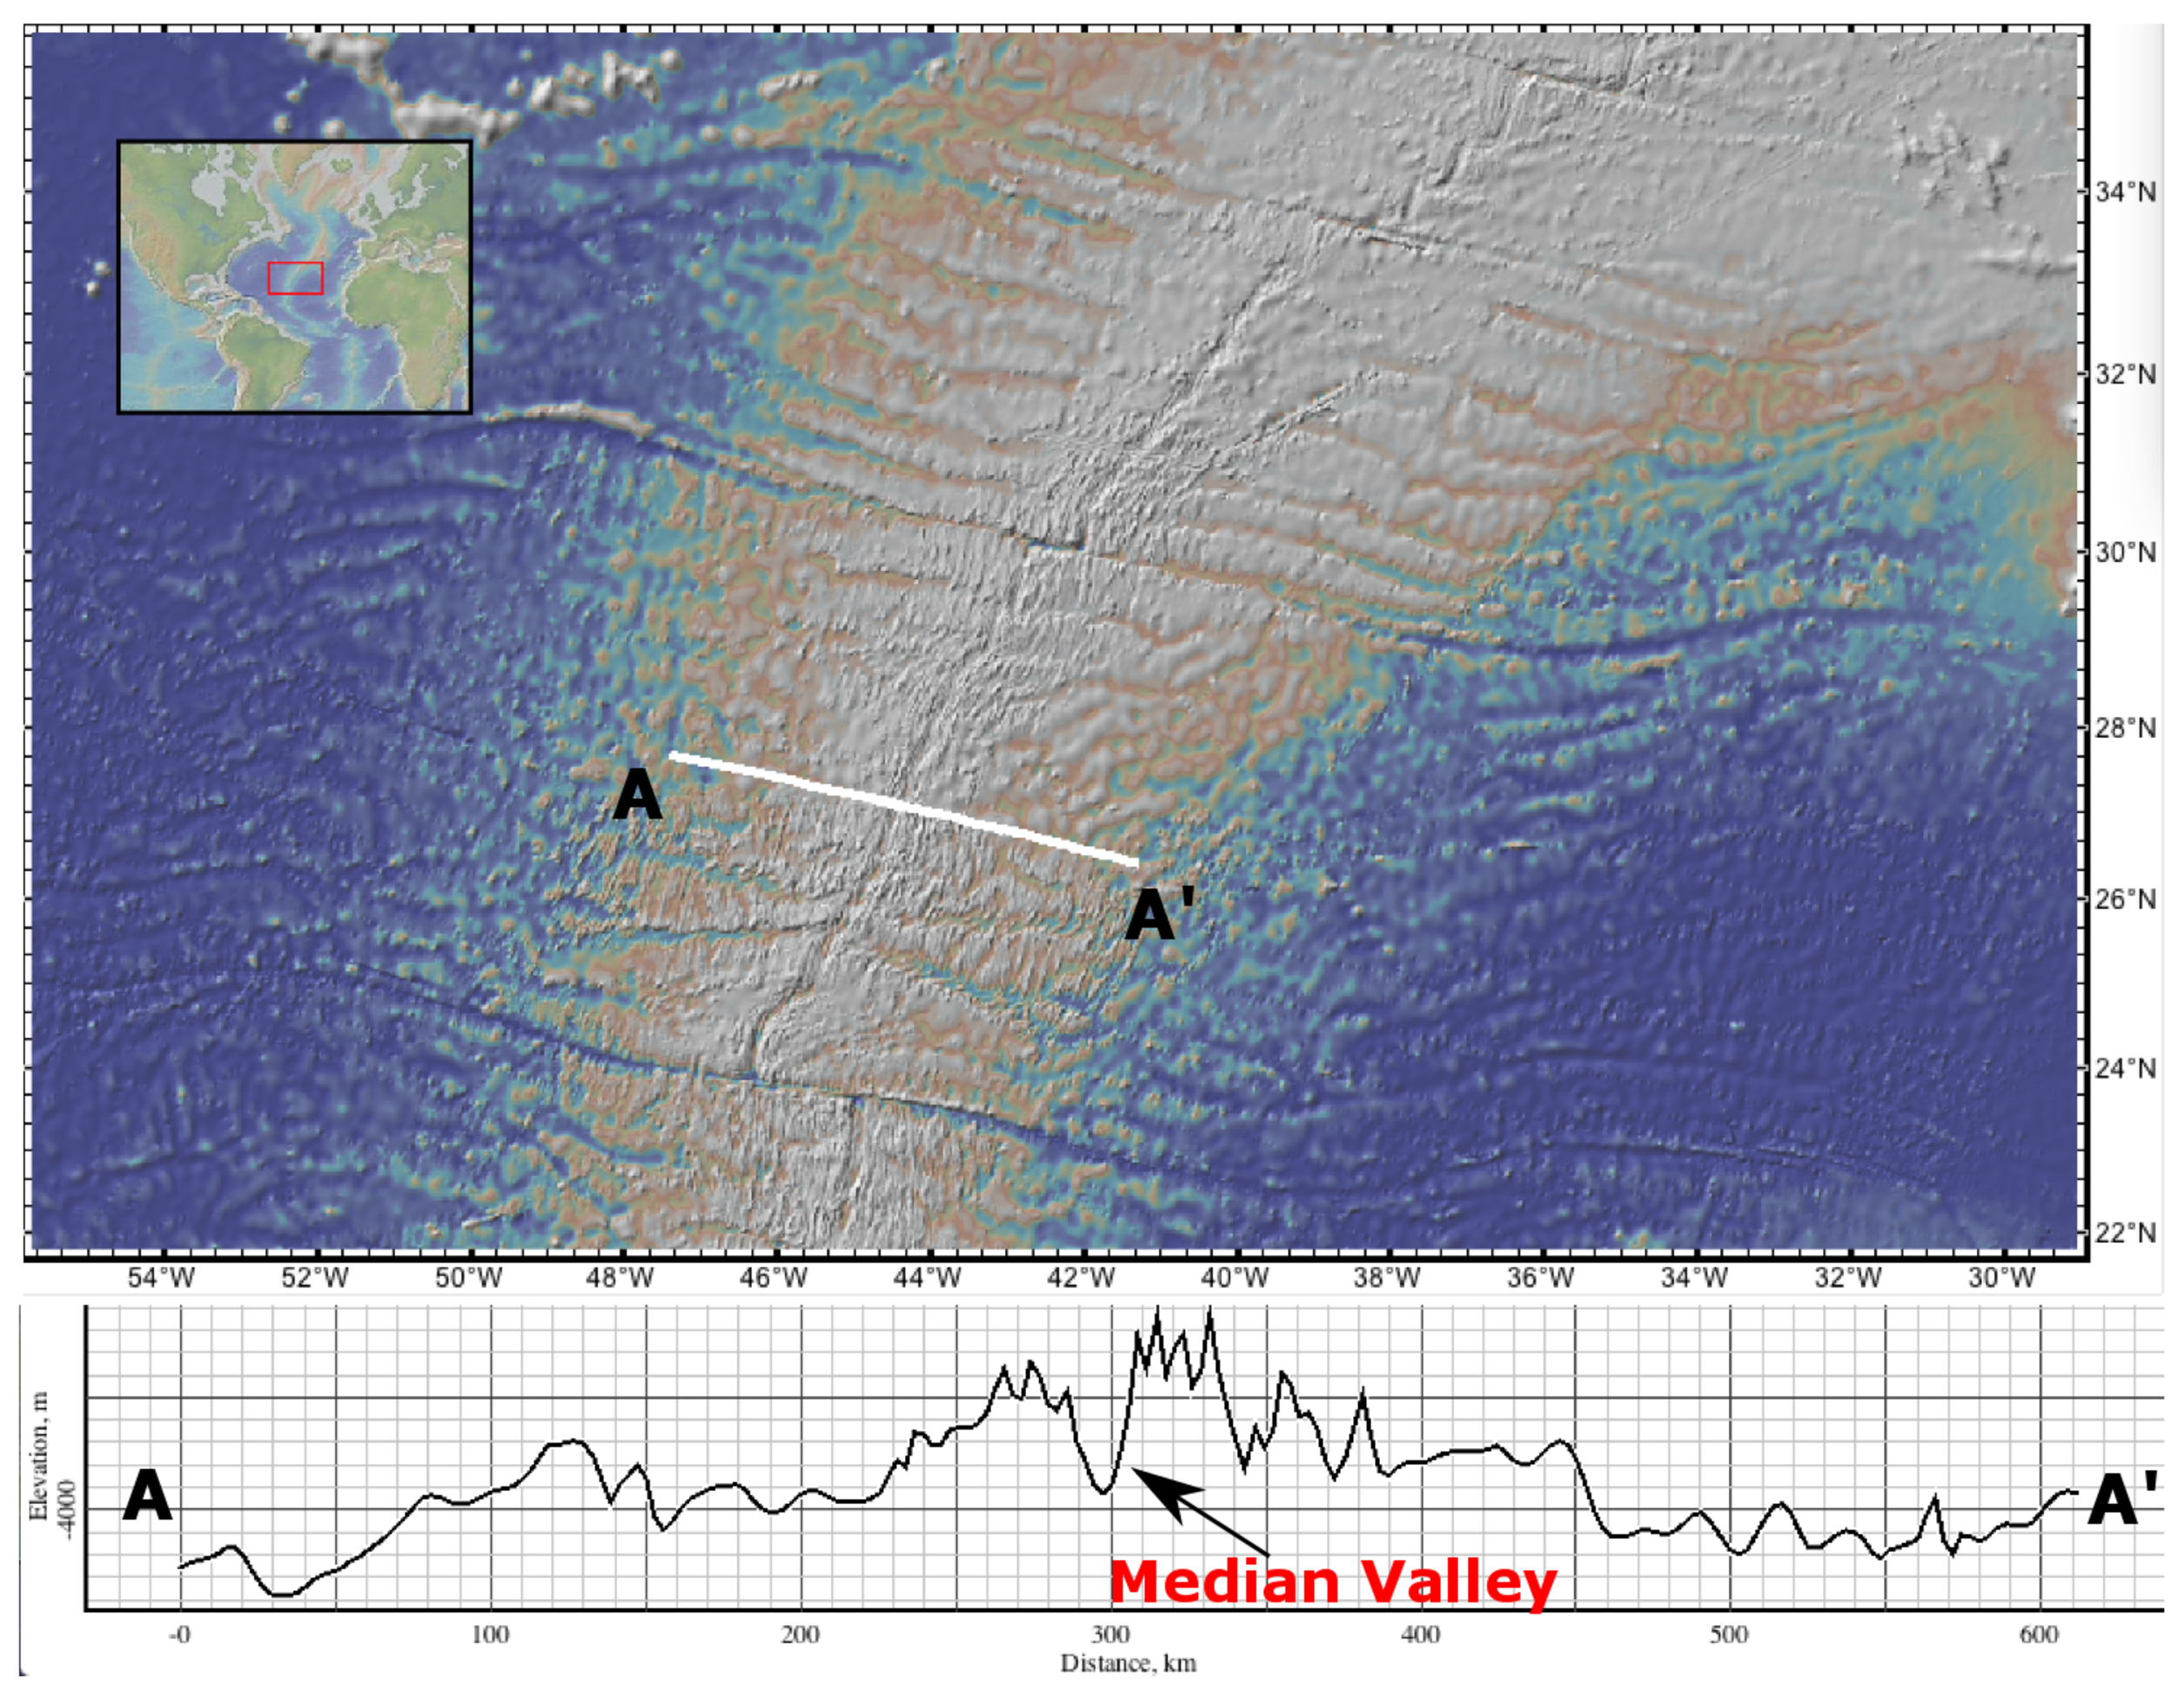
\includegraphics[width=20pc]{./Figures/fig_Intro1_1.eps}
  \caption{Slow spreading Mid-Atlantic Ridge}
  \label{fig_Intro1_1}
\end{figure}

\begin{figure}
\noindent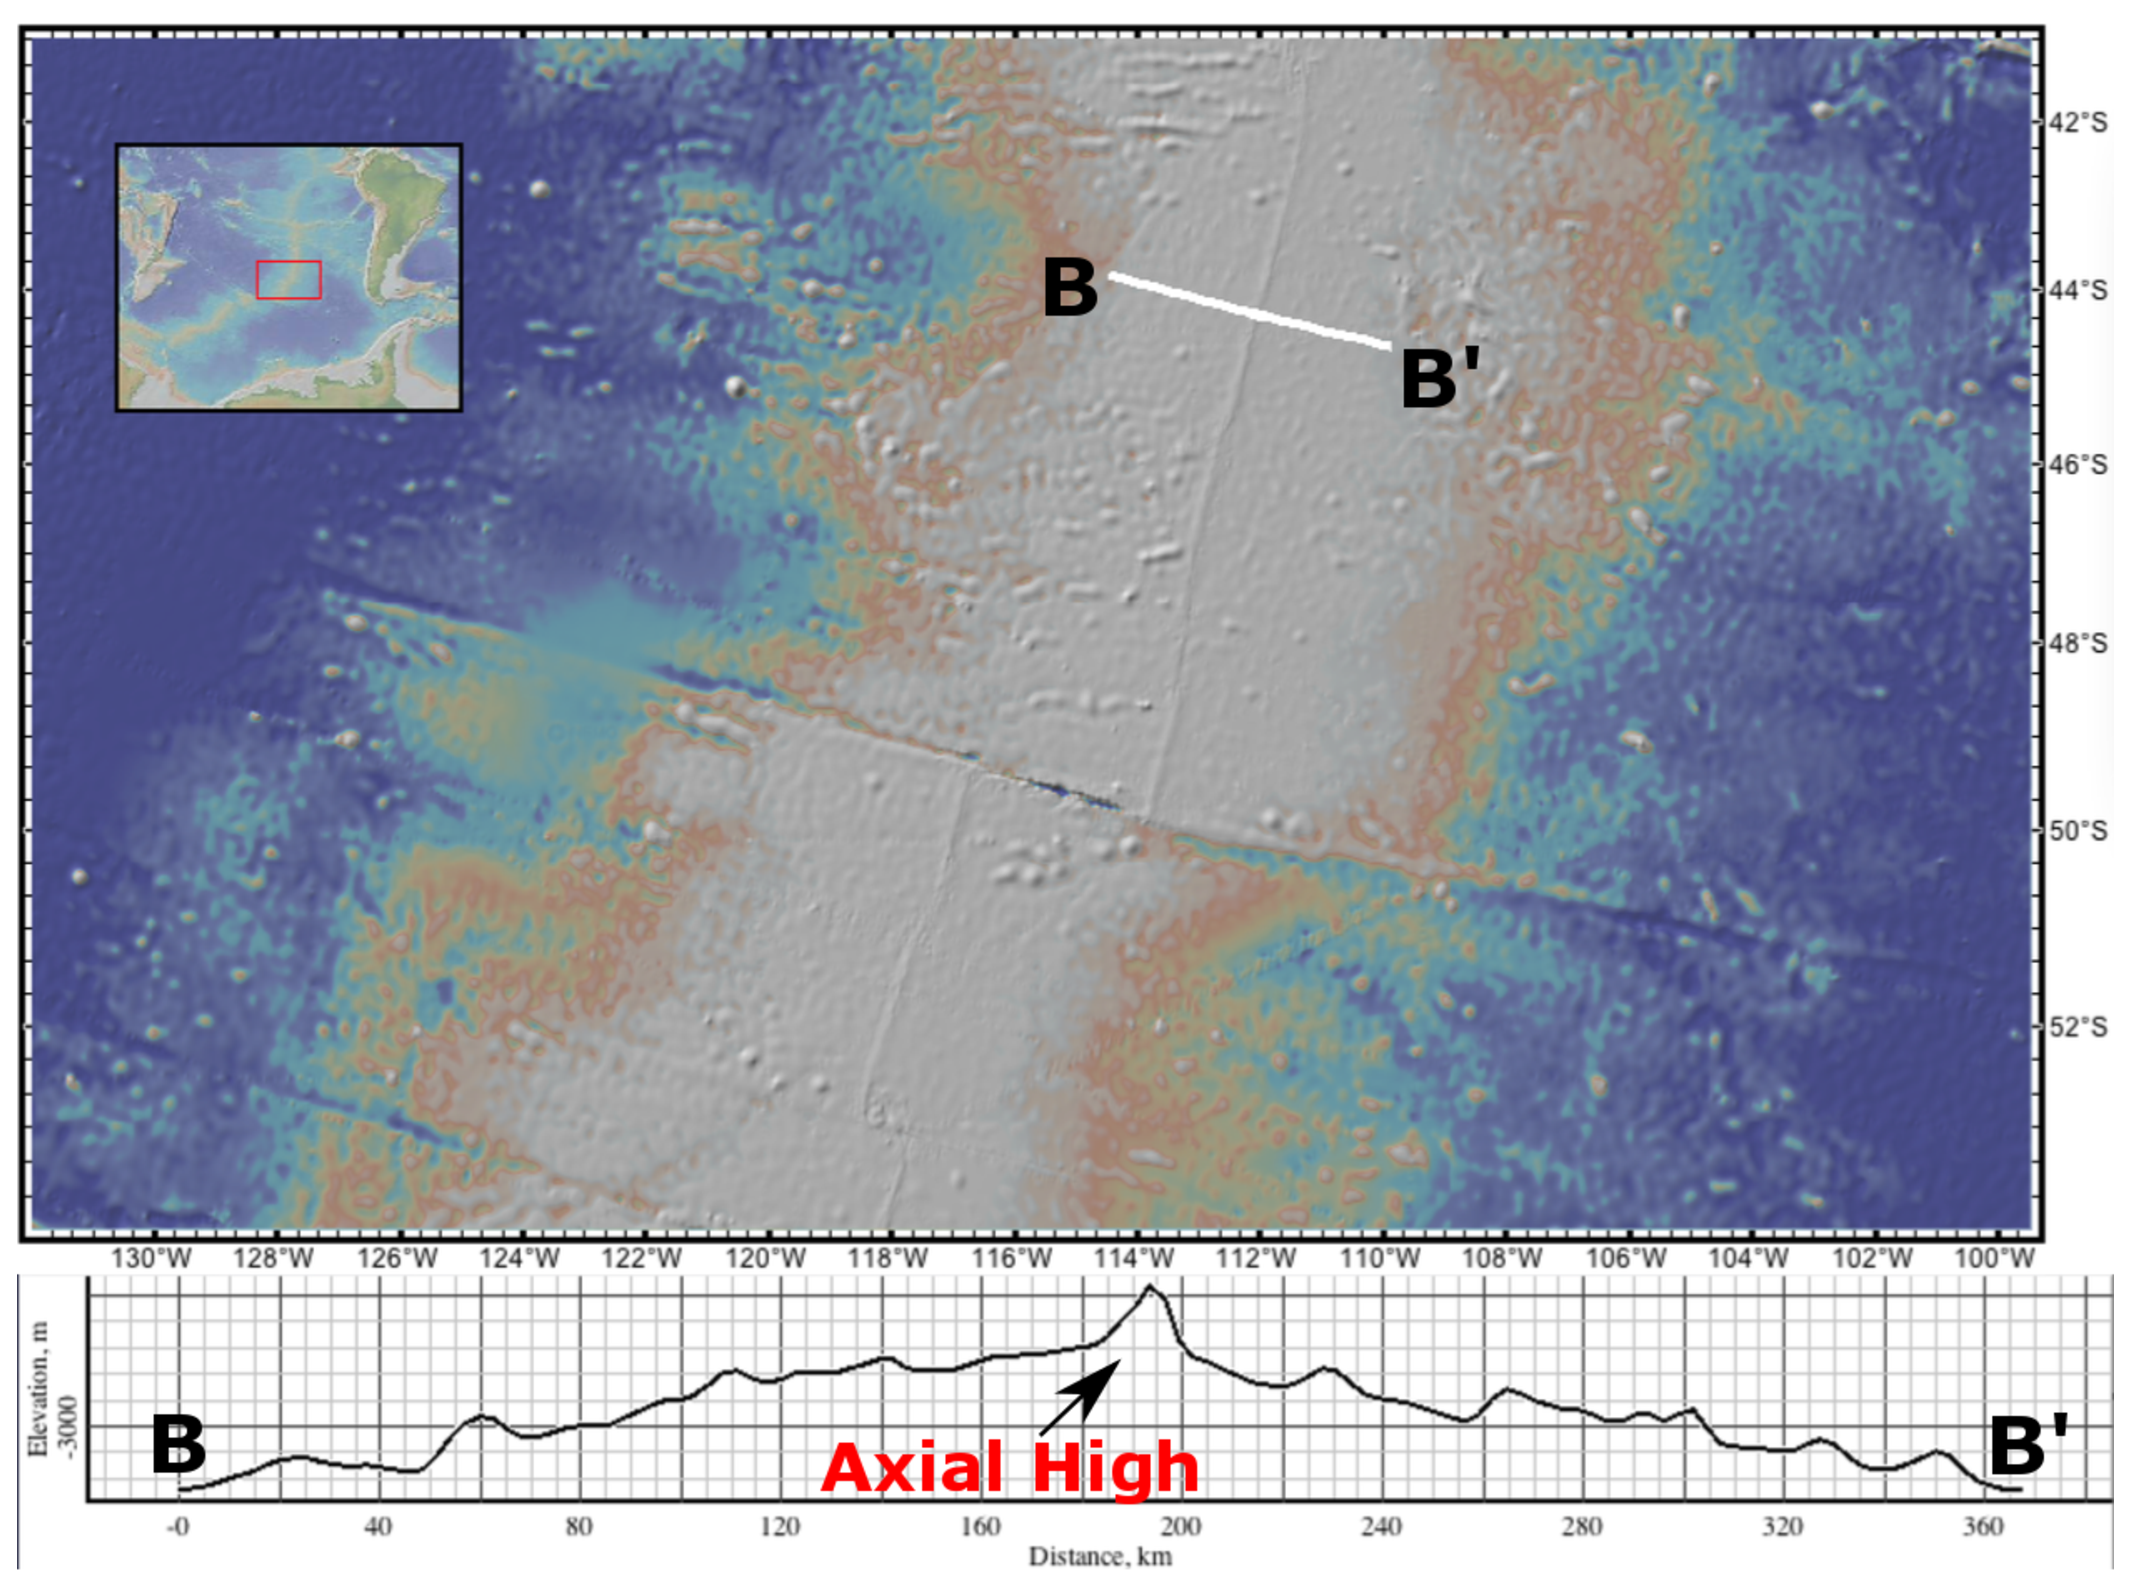
\includegraphics[width=20pc]{./Figures/fig_Intro1_3.eps}
  \caption{Fast spreading East Pacific Rise}
  \label{fig_Intro1_3}
\end{figure}

\begin{figure}[h]
\noindent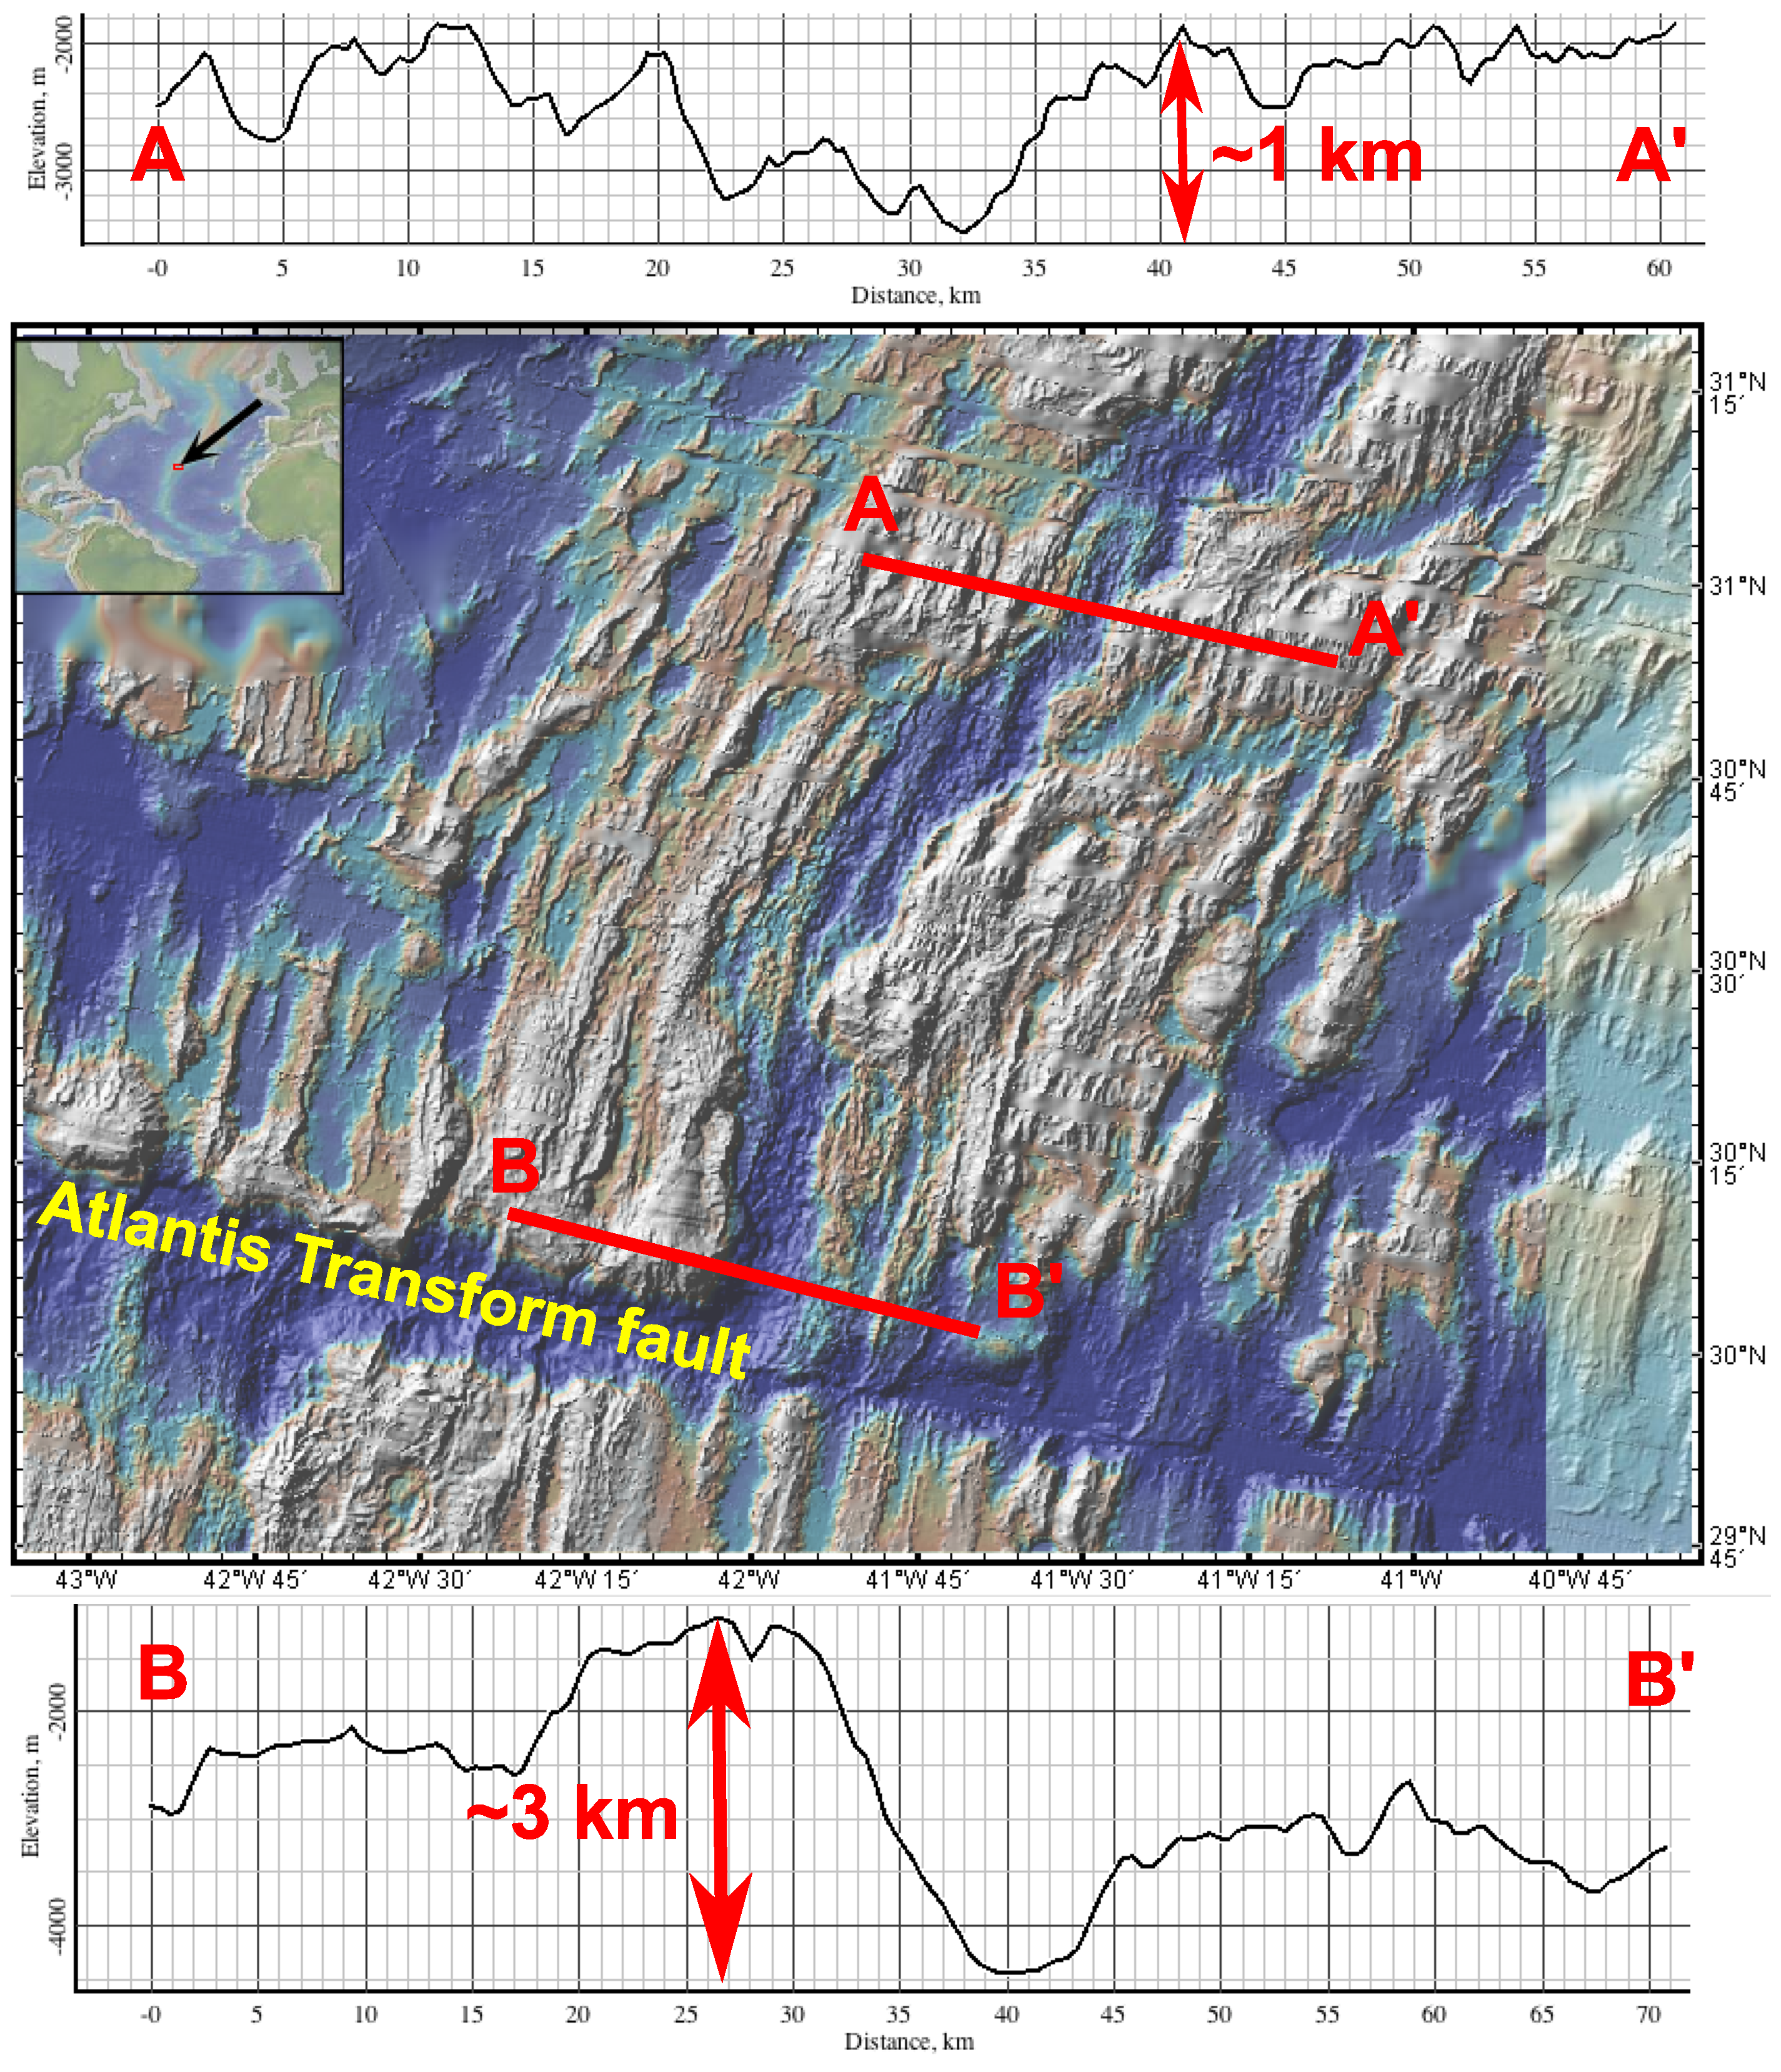
\includegraphics[width=20pc]{./Figures/fig_Intro1_2_30N_MAR_offAxisMorphologies.eps}
 \caption[Two bathymetric profiles across the Mid-Atlantic Ridge around 30$\degree$N with vertical exaggeration of 10.]{Two bathymetric profiles across the Mid-Atlantic Ridge around 30$\degree$N with vertical exaggeration of 10. A-A$^{\prime}$ is closer to the segment center while B-B$^{\prime}$ is at the tip of the segment.}
  \label{fig_Intro2_1}
\end{figure}

\begin{figure}[h]
\noindent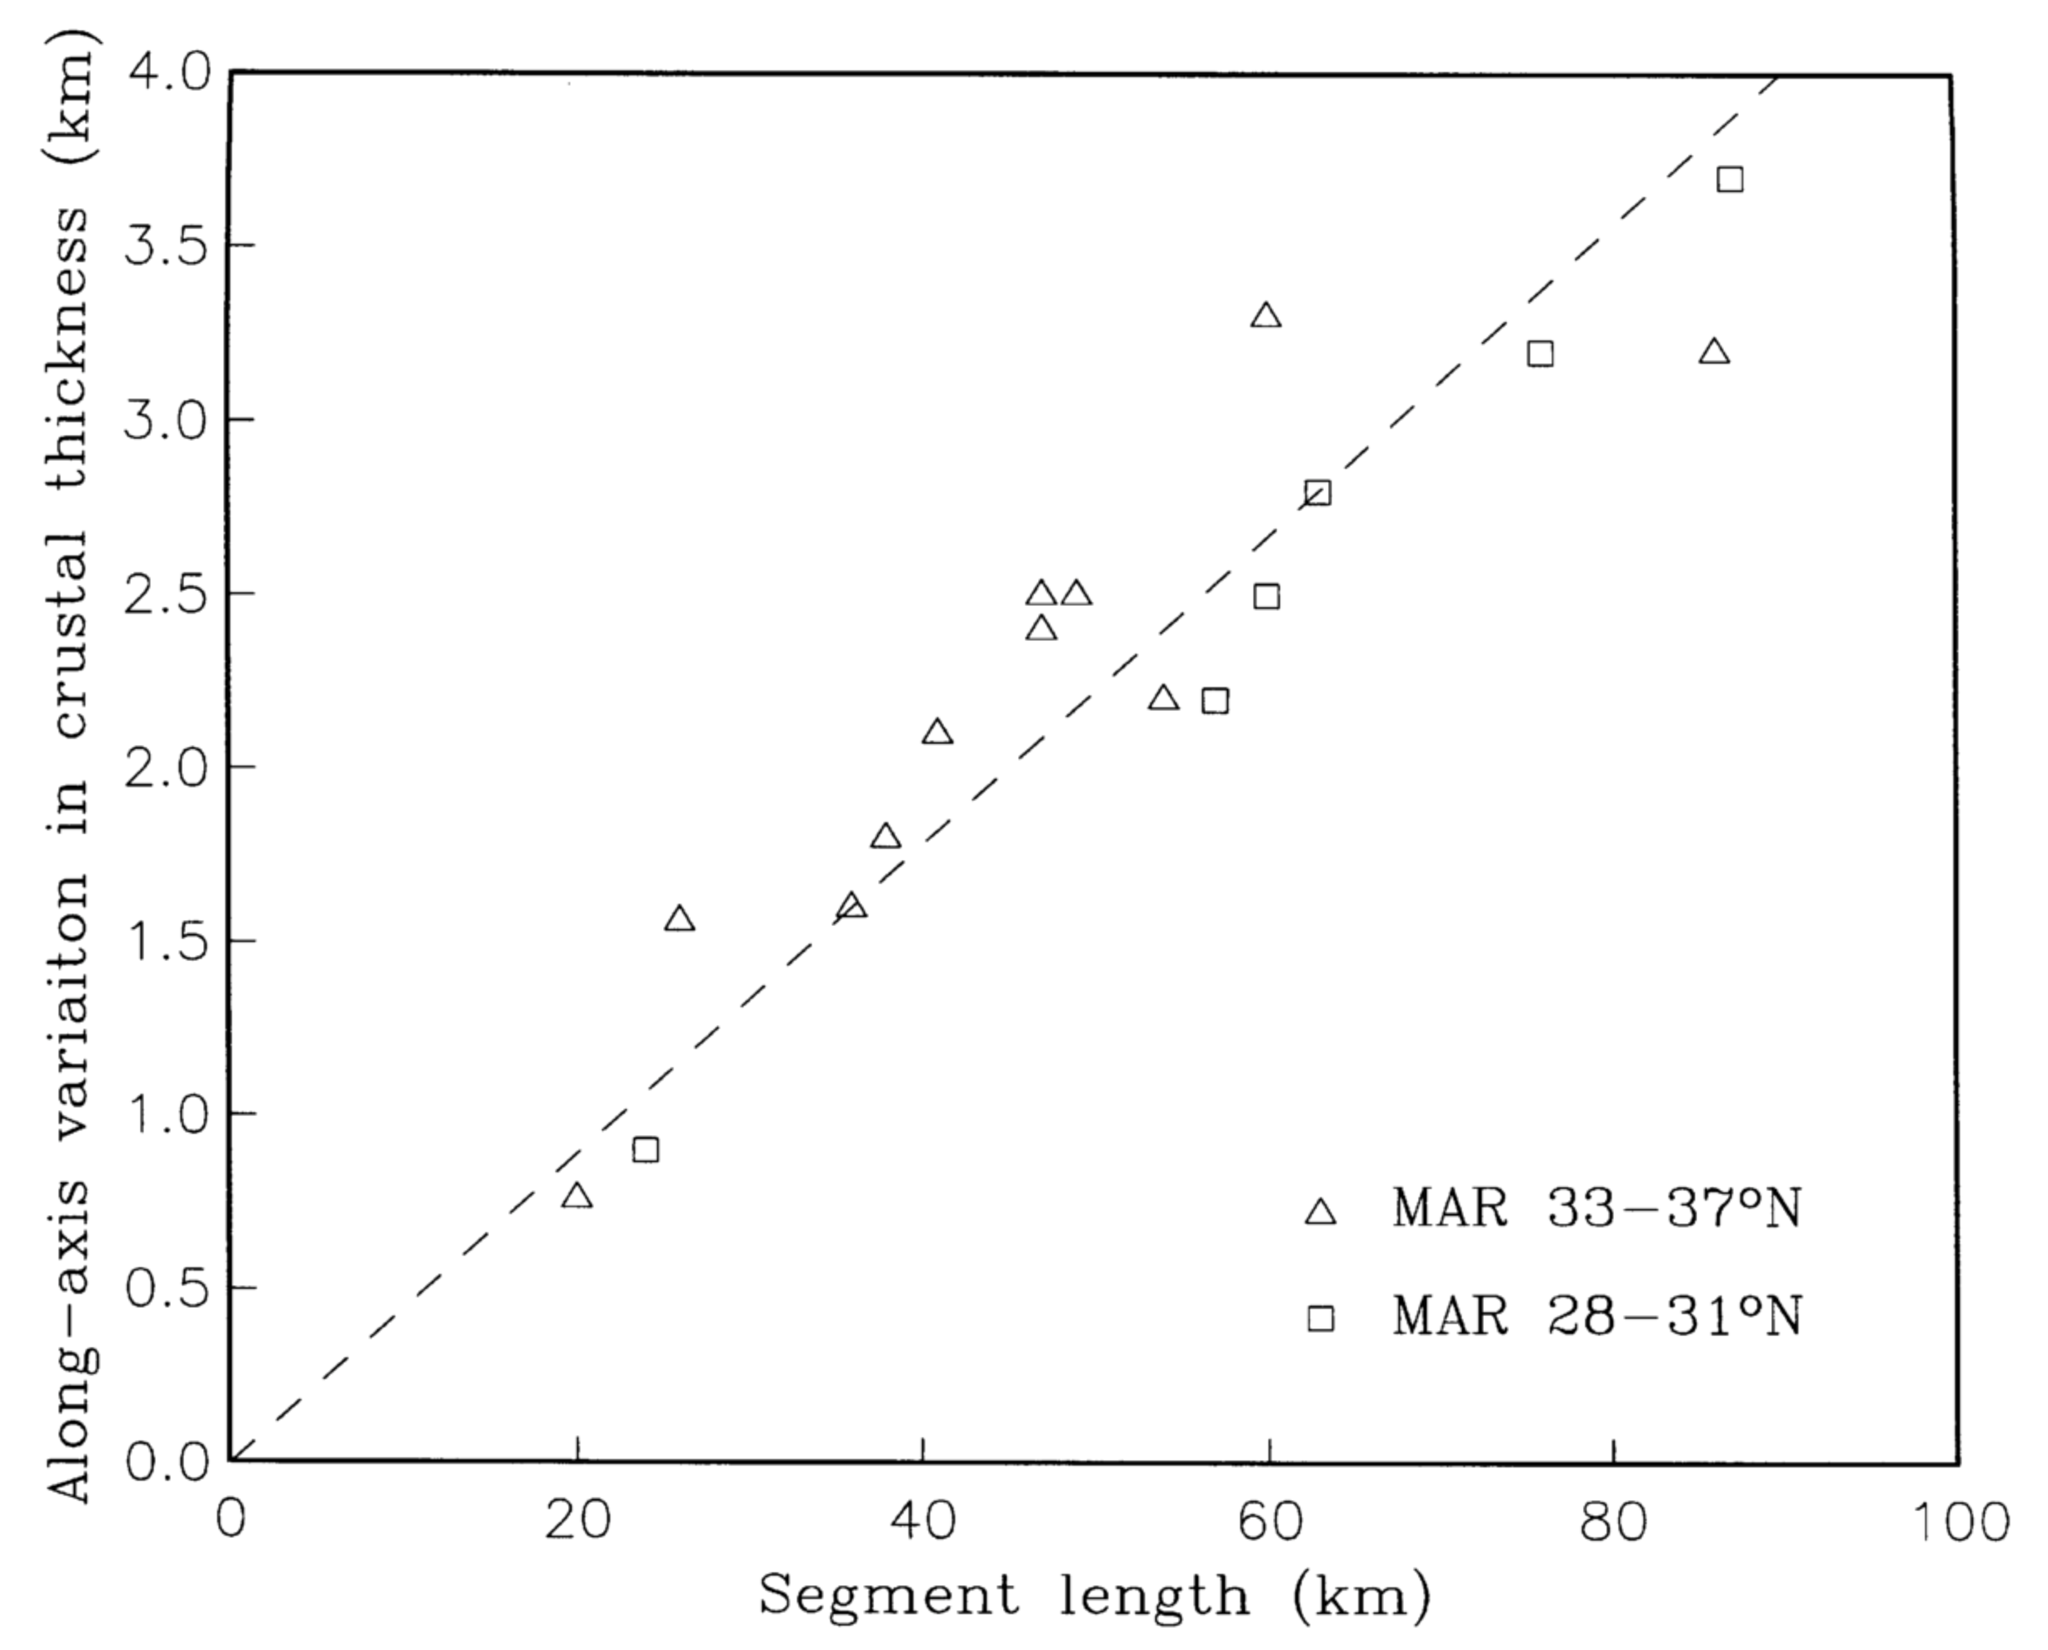
\includegraphics[width=0.5\textwidth]{./Figures/fig_Intro3_1.eps}
 \caption[Relationship between the maximum crustal thickness variations ($\Delta H_{c}$) along a ridge segment and the segment length (L).]{Relationship between the maximum crustal thickness variations ($\Delta H_{c}$) along a ridge segment and the segment length (L). The dashed line is the best-fit linear regression of the combined data \citep{Chen1999}.}
 \label{fig_Intro3_1}
\end{figure}

\begin{figure}[h]
\noindent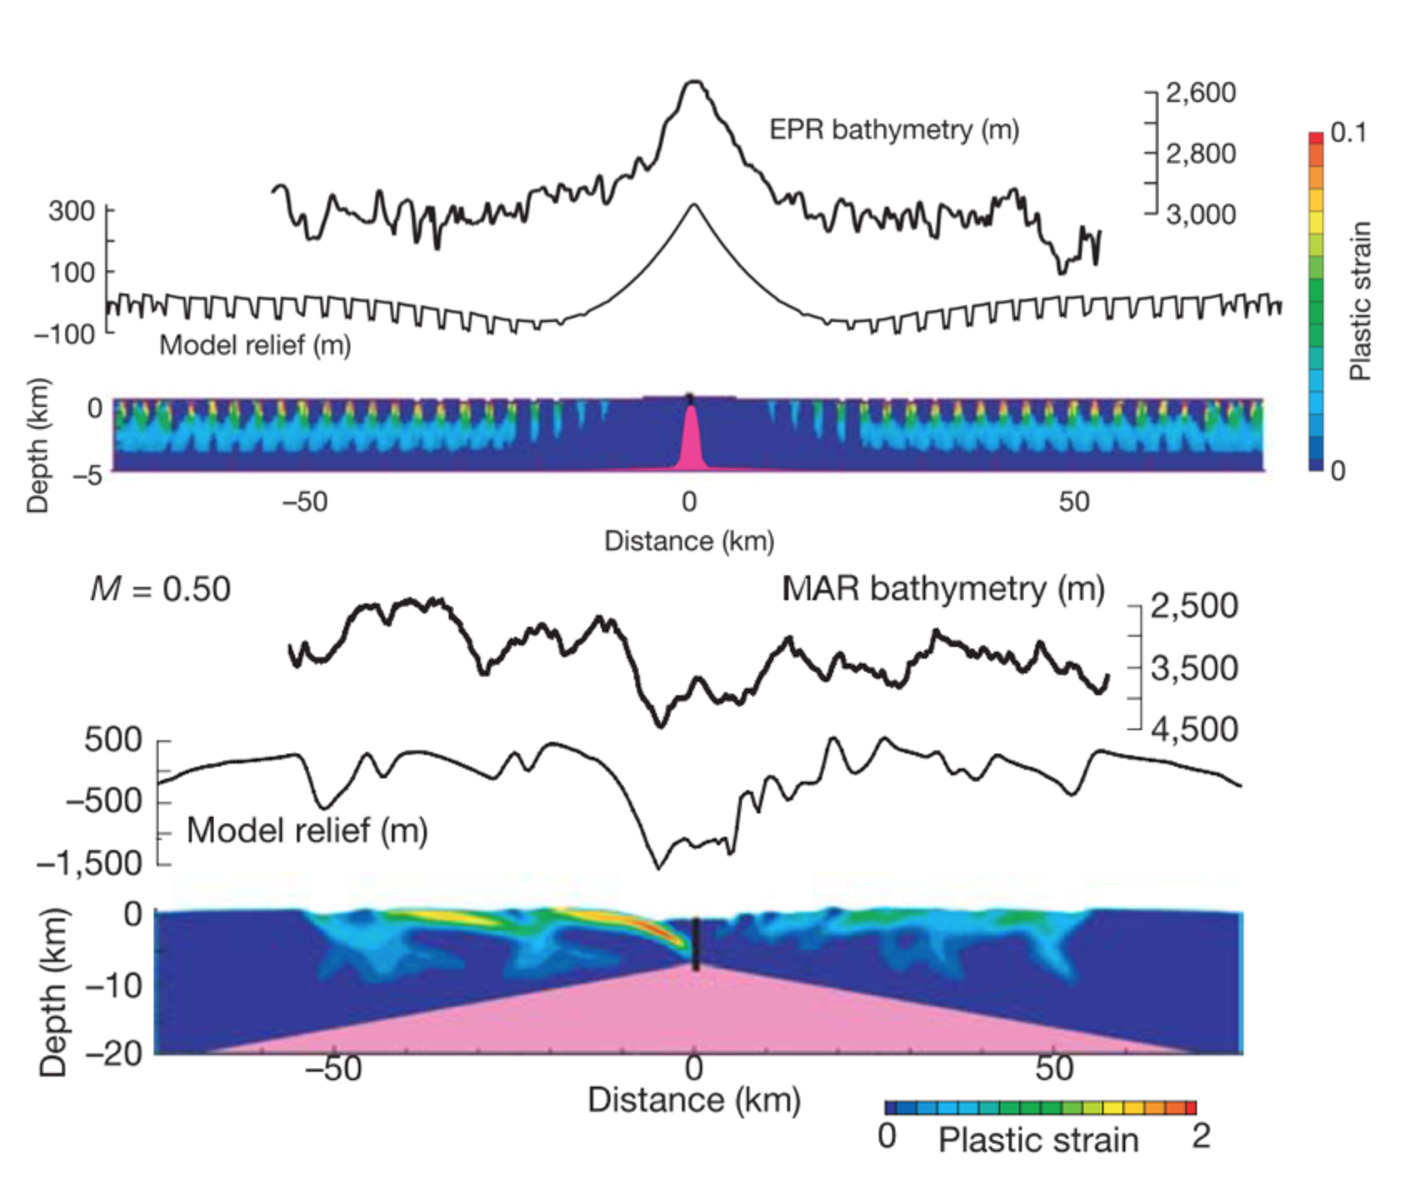
\includegraphics[width=0.8\textwidth]{./Figures/fig_Intro5_1.eps}
 \caption[2D model results adapted from \citep{Buck2005}.]{Upper: modeling result for fast spreading agrees well with East Pacific Rise. Lower: modeling result for slow spreading ridges agrees well with the bathymetry of Mid-Atlantic Ridge. Adapted from \citep{Buck2005}.}
 \label{fig_Intro5_1}
\end{figure}

\begin{figure}[h]
\noindent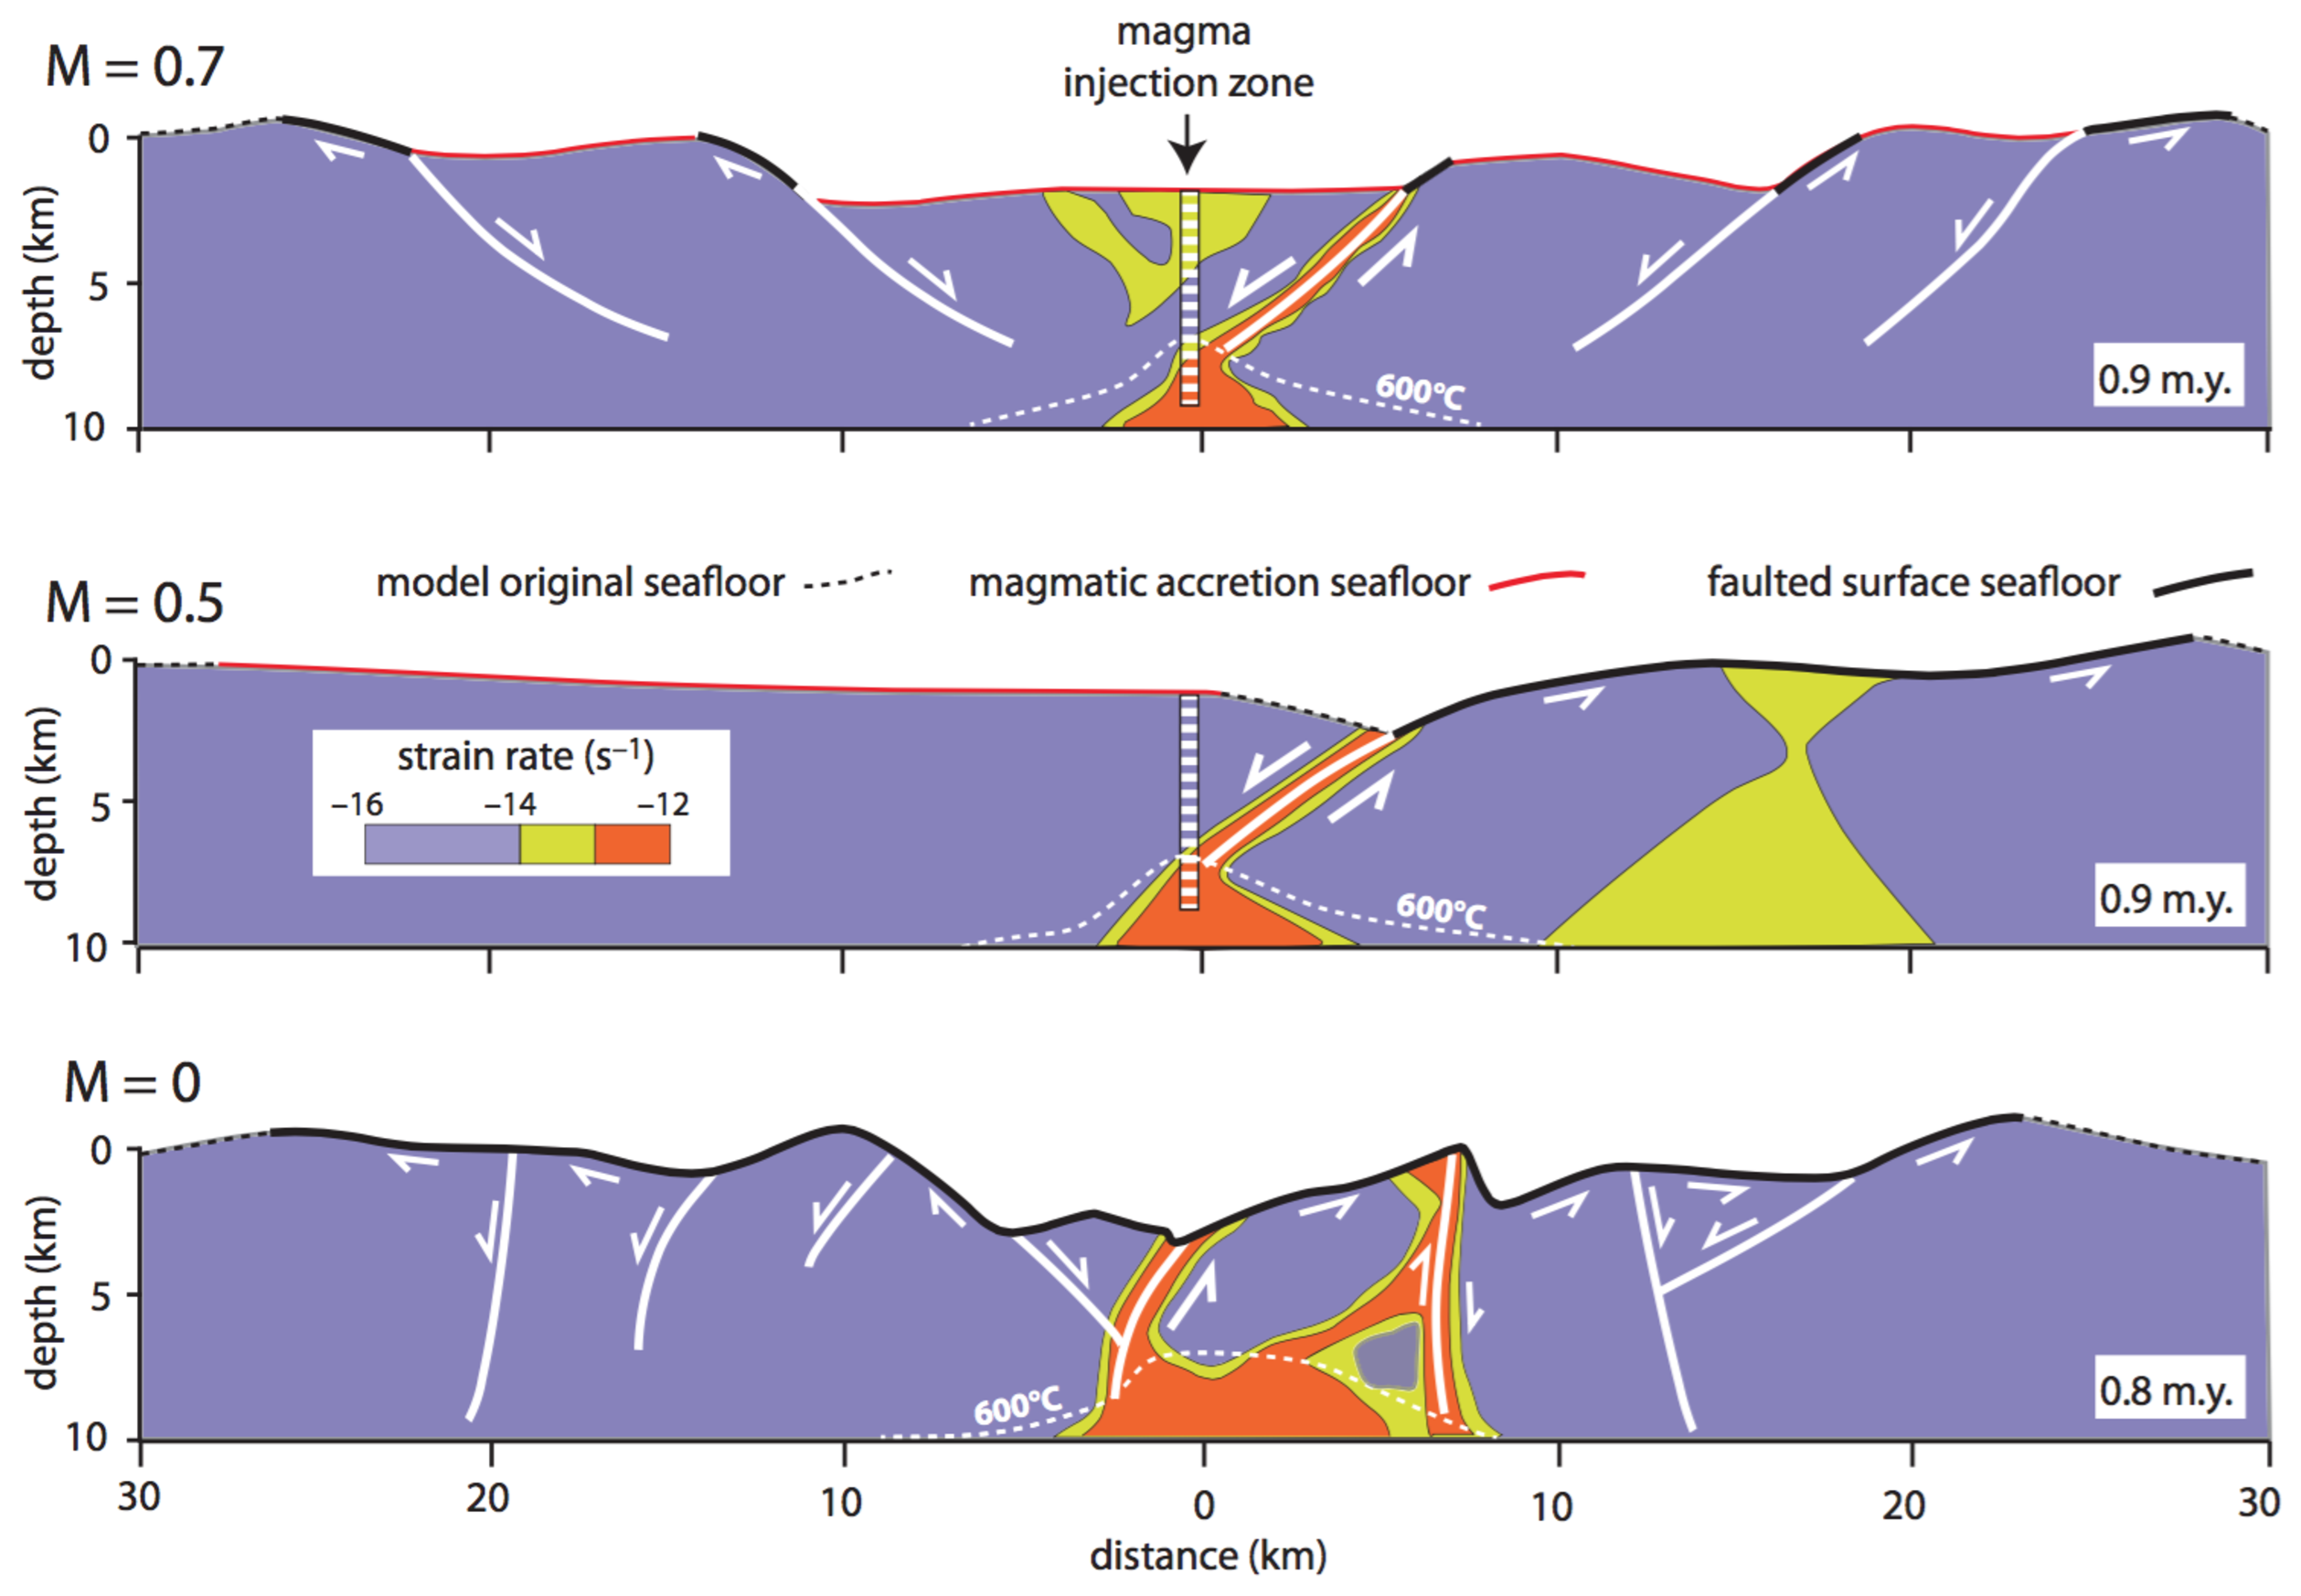
\includegraphics[width=0.8\textwidth]{./Figures/fig_Intro_Tucholke2008.eps}
 \caption[2D model results adapted from \citep{Tucholke2008,Whitney2012}.]{Snapshots of modeled fault behavior and seafloor morphology for M $=$ 0, 0.5, and 0.7; model allows thermal evolution. Structural interpretation is superimposed on modeled distribution of strain rate; model time is indicated in panels at lower right; dashed white line at bottom is 600 $\degree$C isotherm and approximates the brittle-ductile transition; dashed seafloor is original model seafloor, red seafloor is that formed dominantly by magmatic accretion, and solid bold seafloor is fault surface. Adapted from [\citealp{Tucholke2008,Whitney2012}].}
 \label{fig_Intro6_1}
\end{figure}

\begin{figure}[h]
\noindent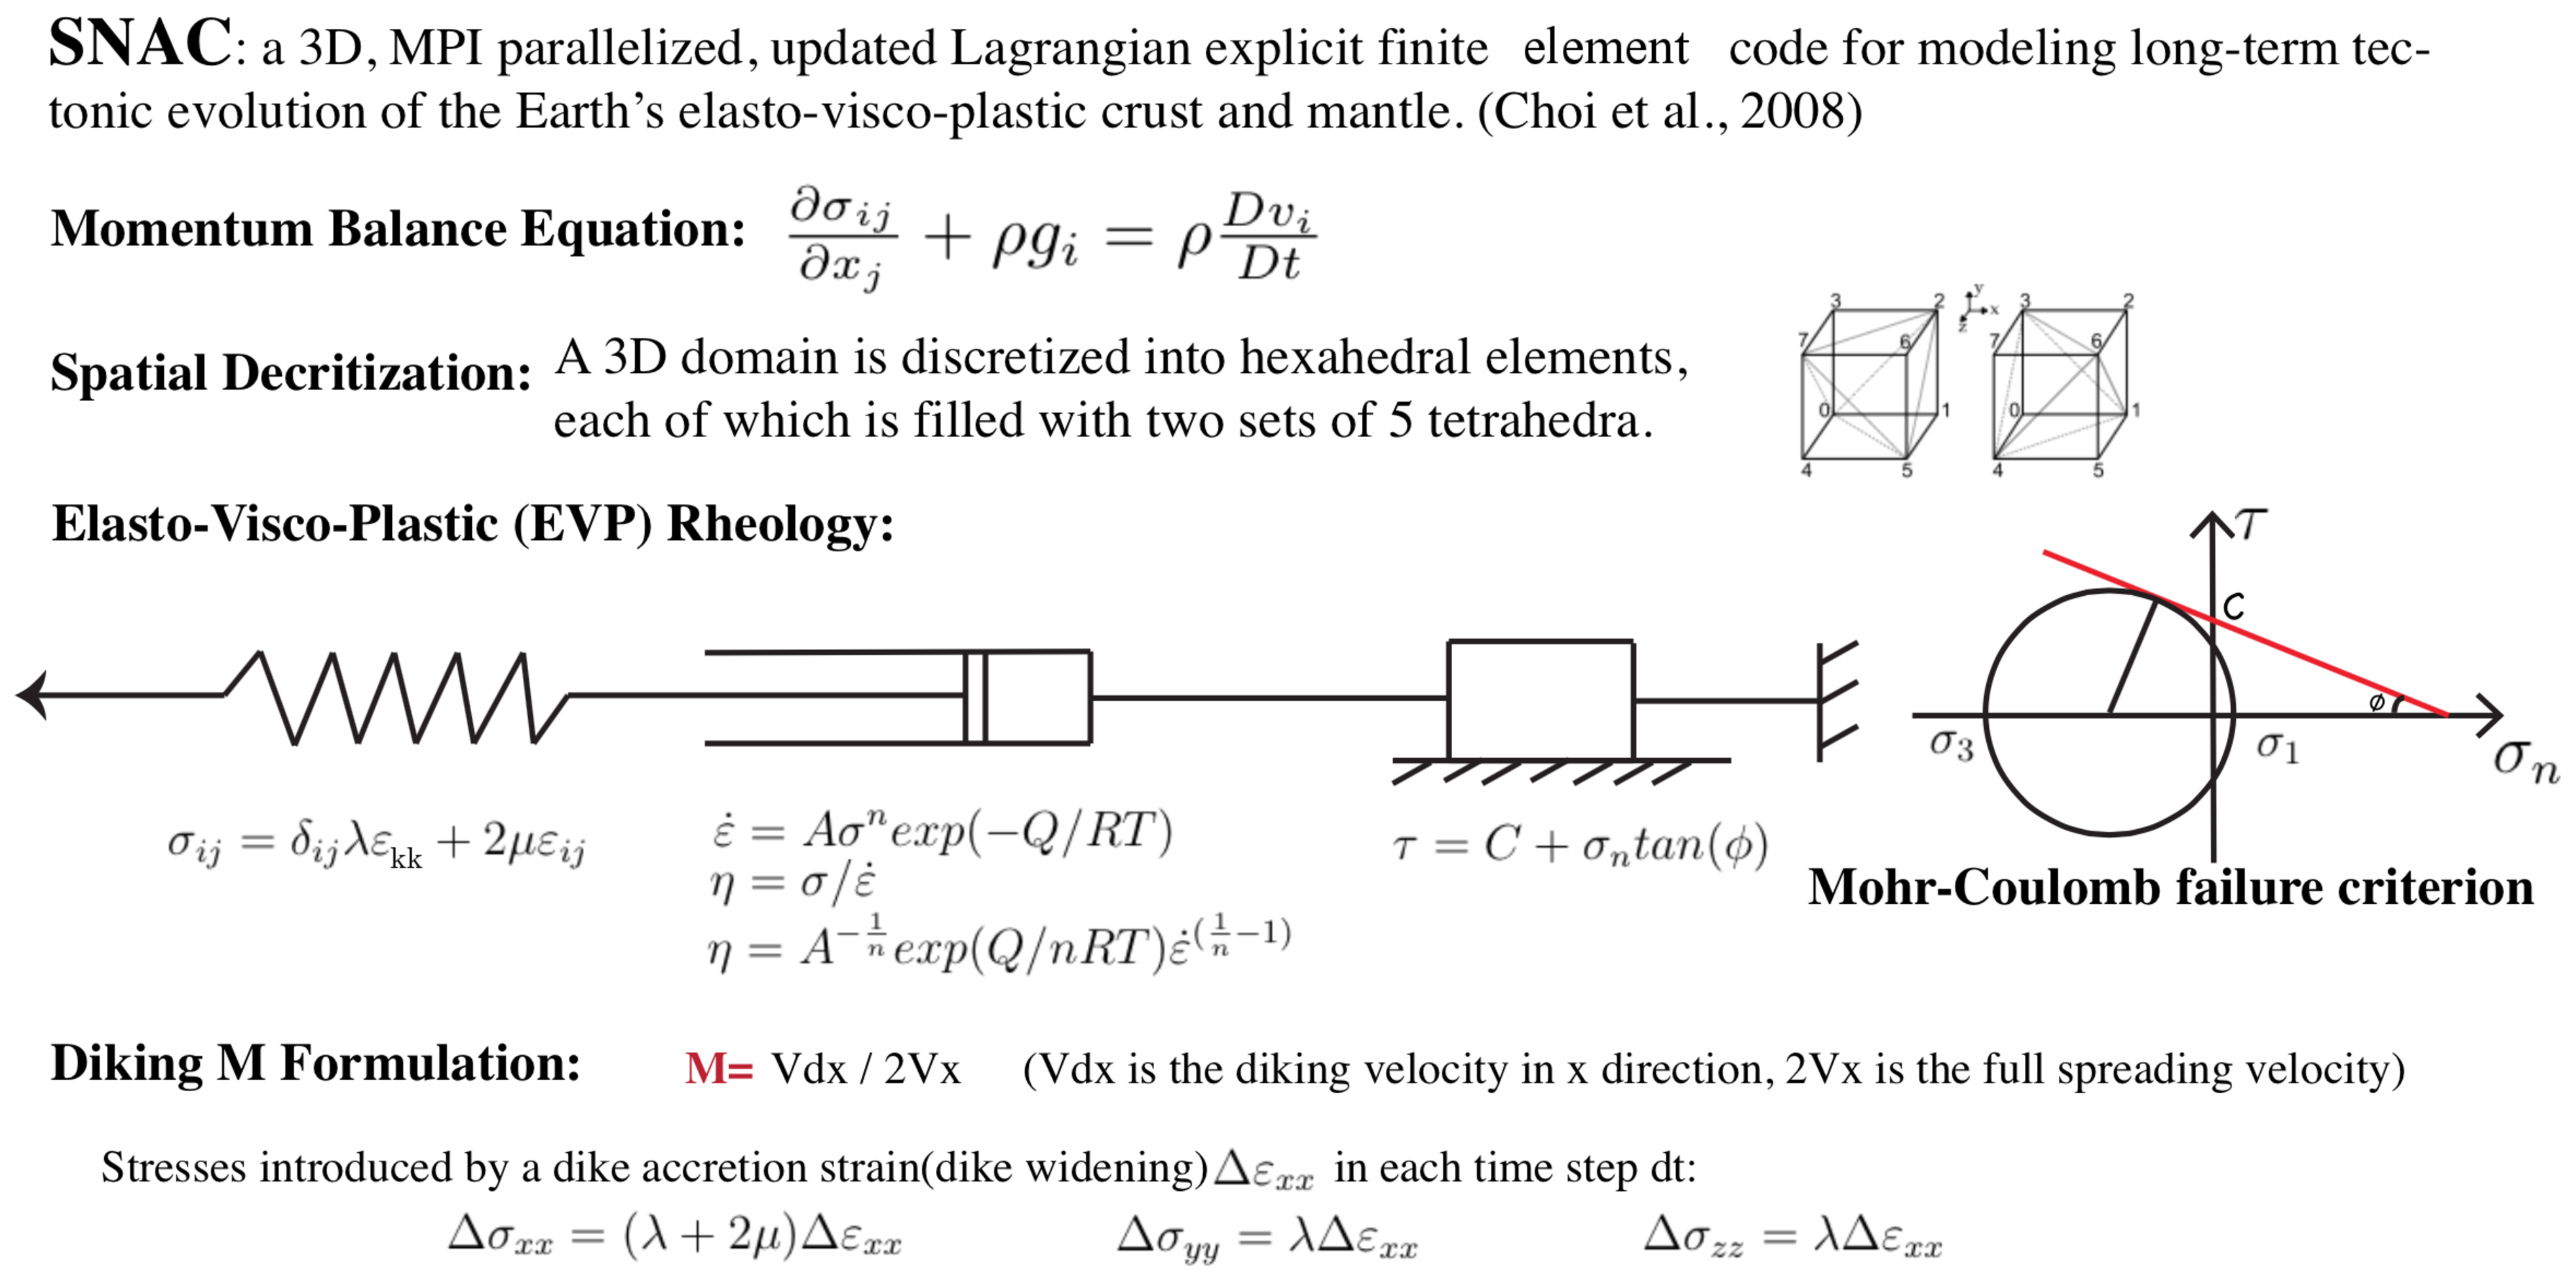
\includegraphics[width=1.0\textwidth]{./Figures/fig_Methods7_3.eps}
 \caption{Essential components of the numerical method.}
 \label{fig_Methods7_3}
\end{figure}

\begin{figure}[h]
\noindent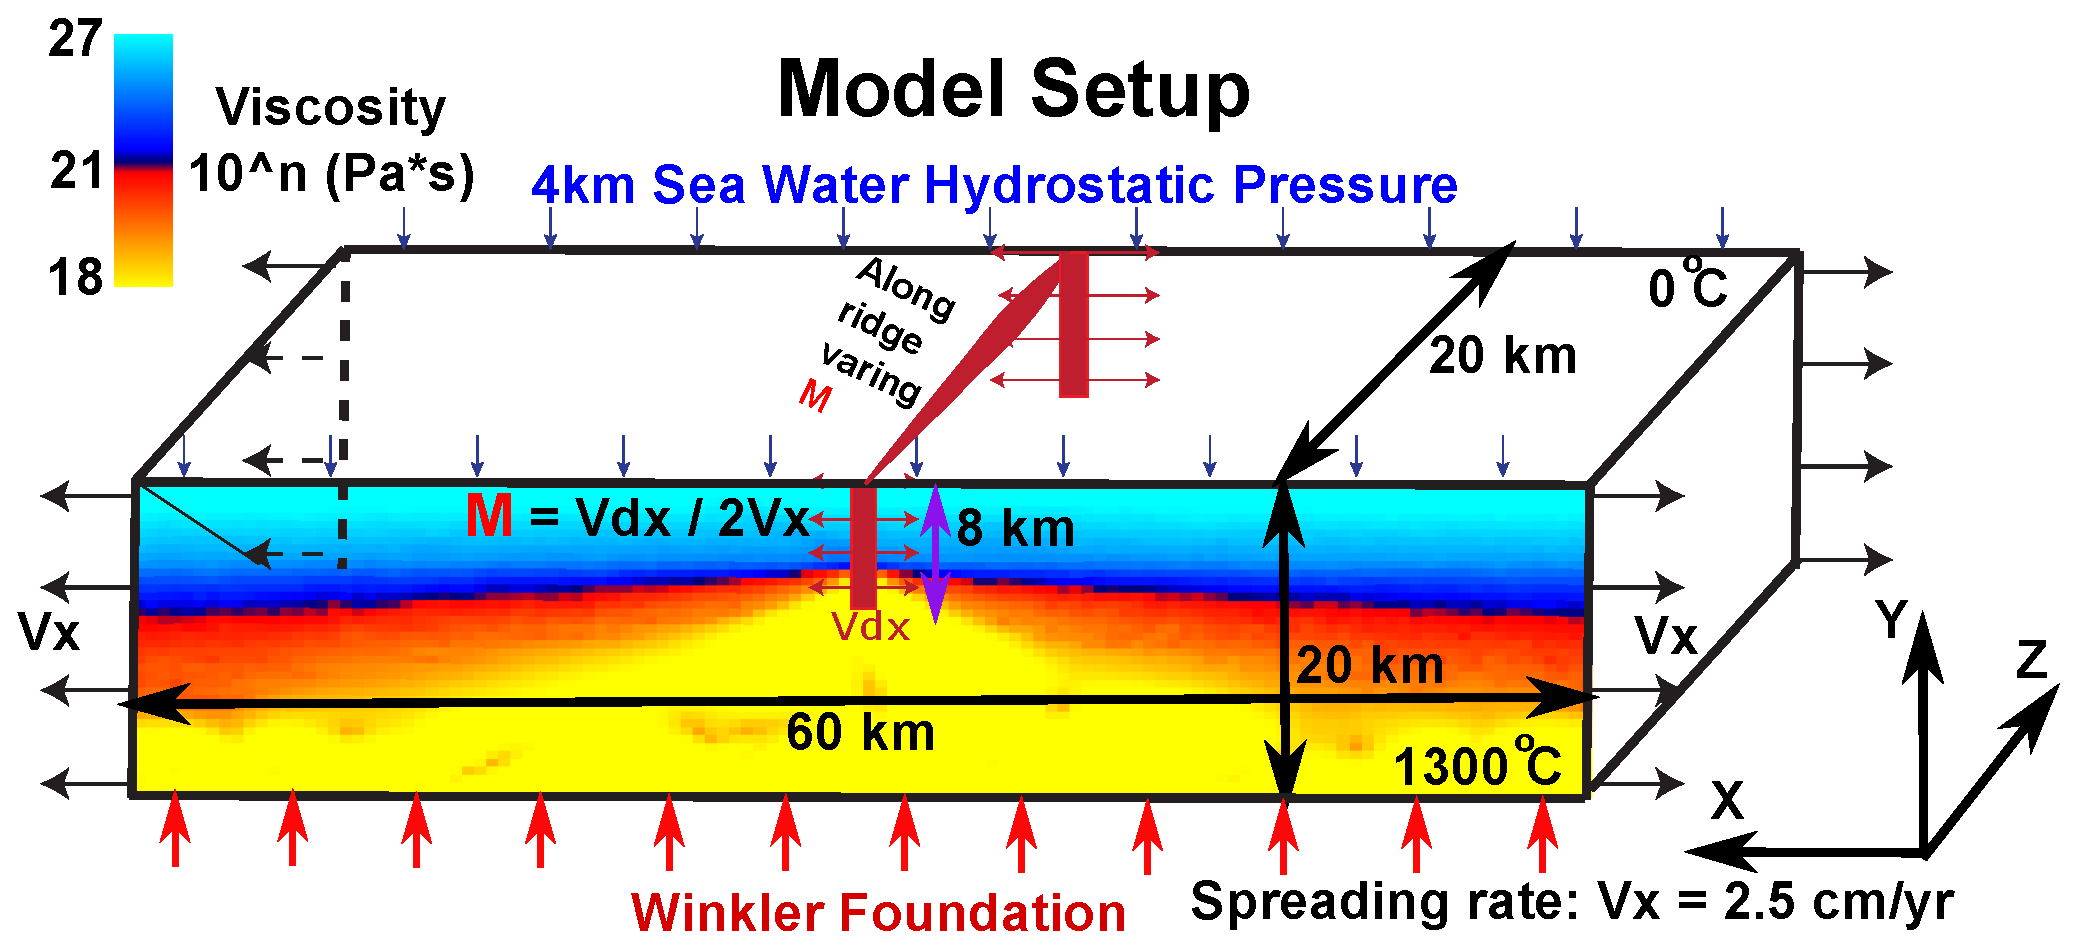
\includegraphics[width=1.0\textwidth] {./Figures/fig_Methods_Model_Setup.eps}
 \caption{Model setup.}
 \label{fig_Methods8_1}
\end{figure}

\begin{figure}[h]
\noindent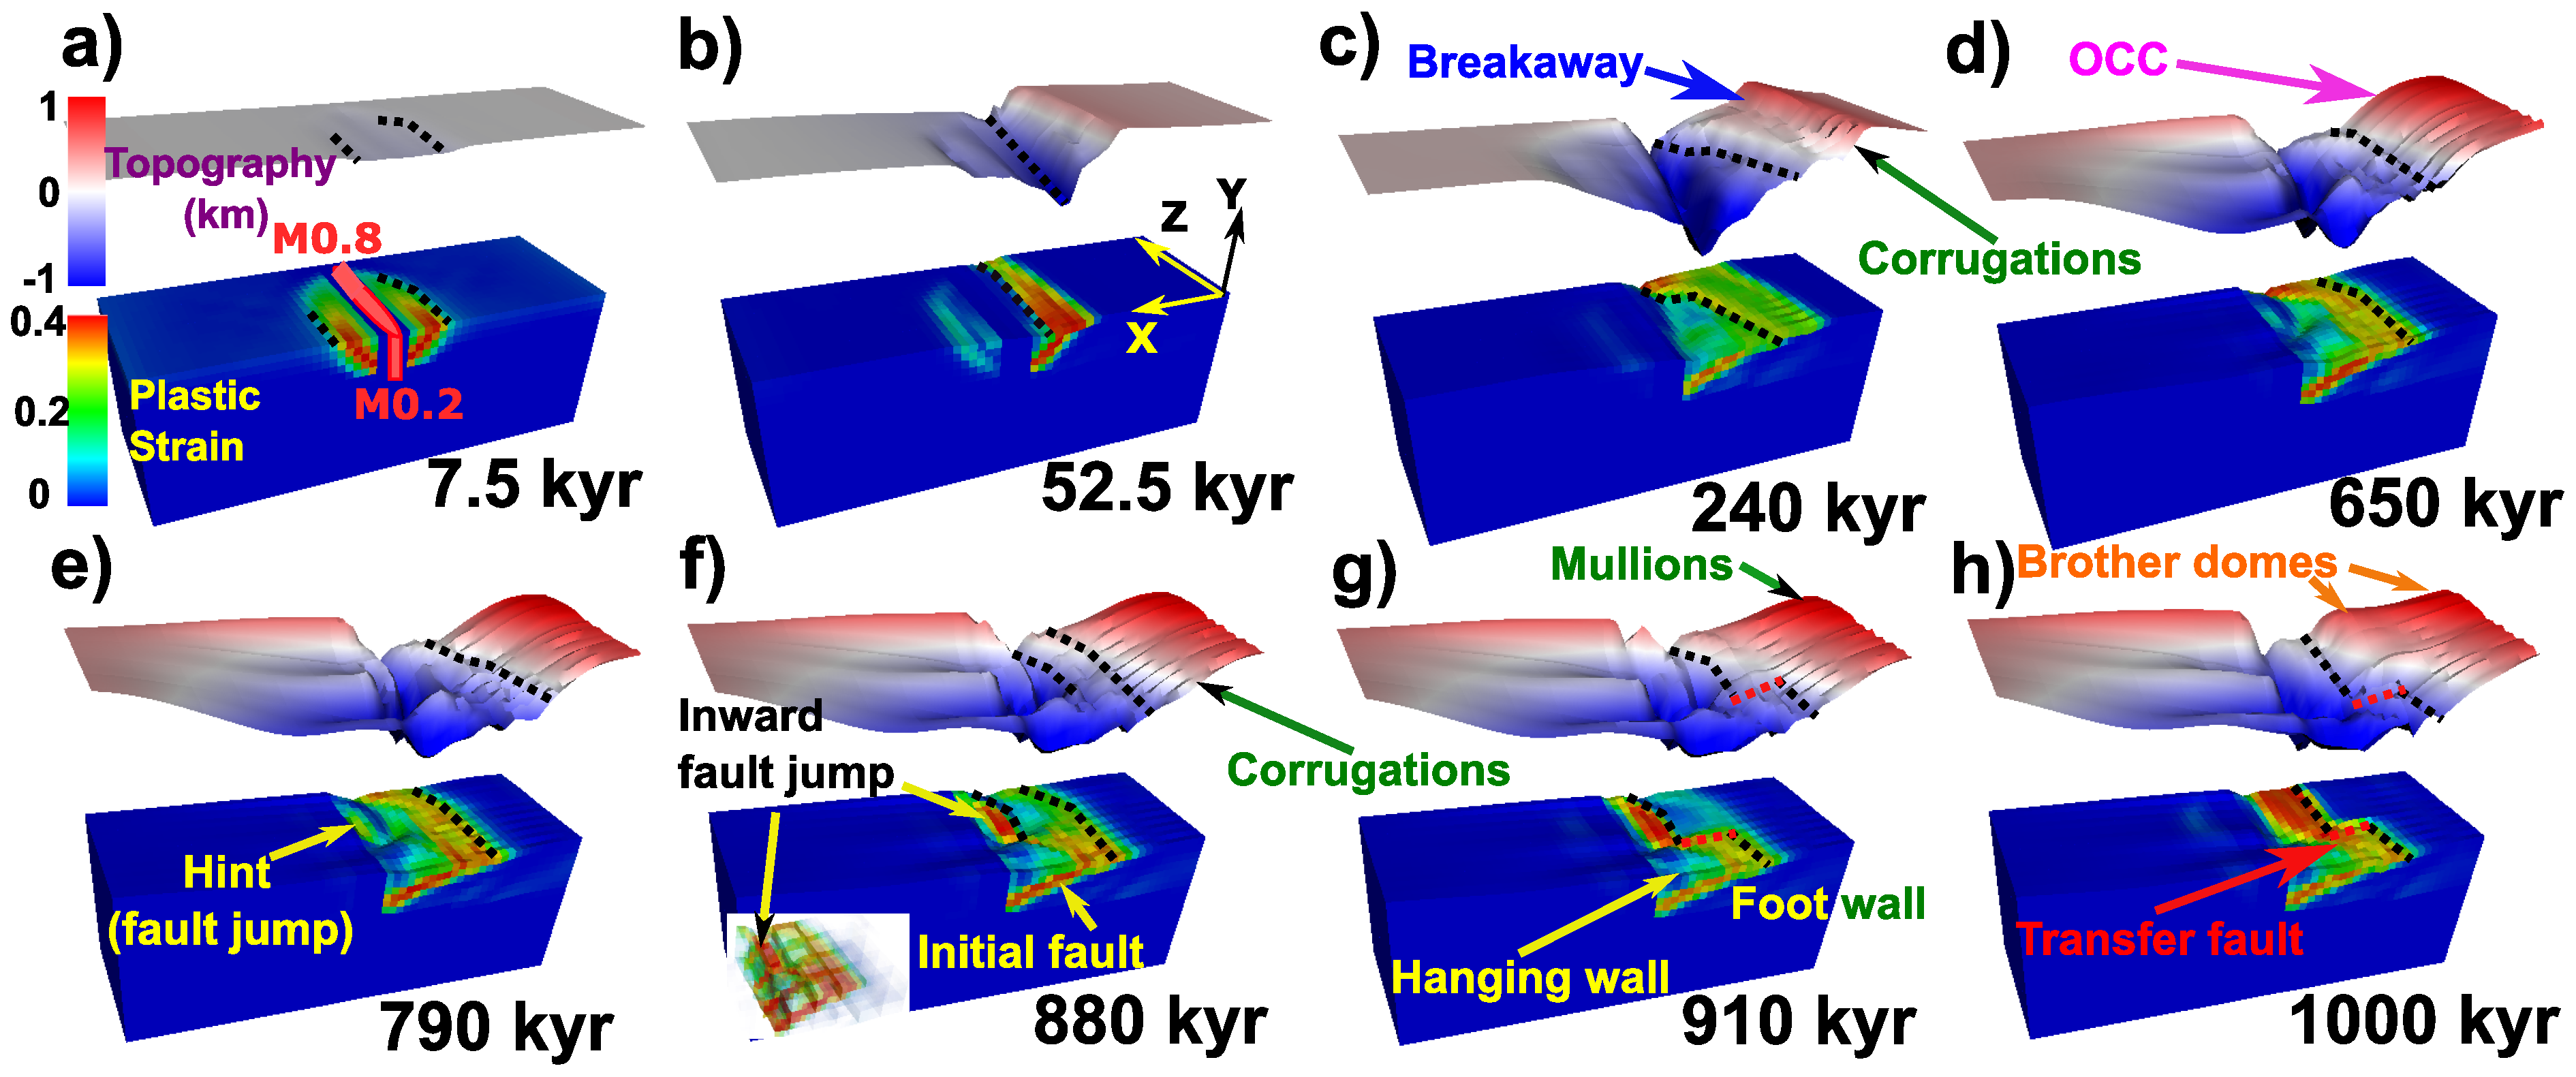
\includegraphics[width=1.0\textwidth]{./Figures/fig_Results_1_reference_model.eps}
  \caption[Reference model M28LinT1.]{Evolution of plastic strain and surface topography of the reference model M28LinT1. Each snapshot shows plastic strain plotted on the model domain, the five times vertically exaggerated topography and the time at which it is taken. The initial seafloor is at 0 km of elevation. The black dashed lines are the terminations of faults. The red dashed lines in g) and h) are the transfer faults that connect the terminations. The inset in f) plots plastic strain with opacity linearly proportional to plastic strain value.}
 \label{fig_Results1_1}
\end{figure}   

\begin{figure}[h]
\noindent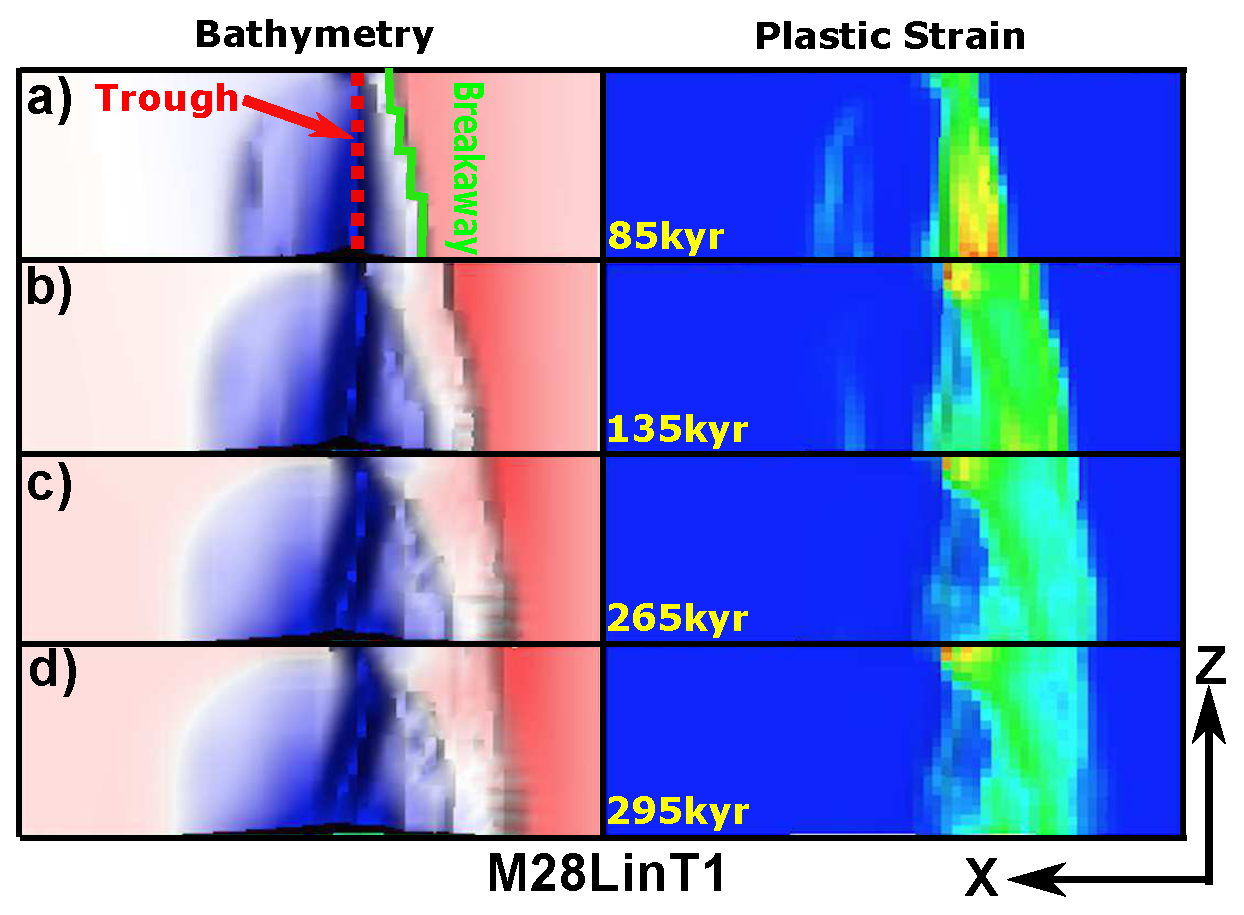
\includegraphics[width=0.6\textwidth]{./Figures/fig_Results1_4.eps}
   \caption[Bird's-eye view of a breakaway in the reference model.]{Bird's-eye view of a breakaway in the reference model at a) 85 kyr, b) 135 kyr, c) 265 kyr and d) 295 kyr. The breakaway is marked by green solid line in a). A narrow zone of depressed topography (``trough'') is marked by red dashed line inside the medain valley (blue area) in a). Color scales are the same with those in Figure~\ref{fig_Results1_1}.}
  \label{fig_Results1_4}
\end{figure}

\begin{figure}[h]
\noindent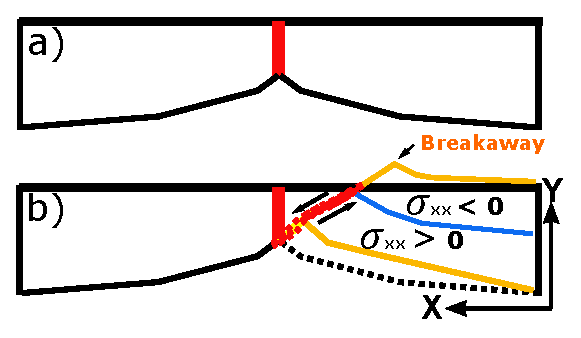
\includegraphics[width=0.6\textwidth]{./Figures/fig_Results4_8_sqrt_cut_back_bending_cartoon.eps}
   \caption[Illustration of bending stresses in lithosphere associated with faulting at the MOR.]{Illustration of the development of bending stress in lithosphere associated with faulting at the MOR. The blue line is the neutral plane where $\sigma_{xx}=0$. Above the neutral plane is compression ($\sigma_{xx}<0$) and beneath it is tension ($\sigma_{xx}>0$).}
  \label{fig_Results4_8}
\end{figure}

\begin{figure}[h]
\noindent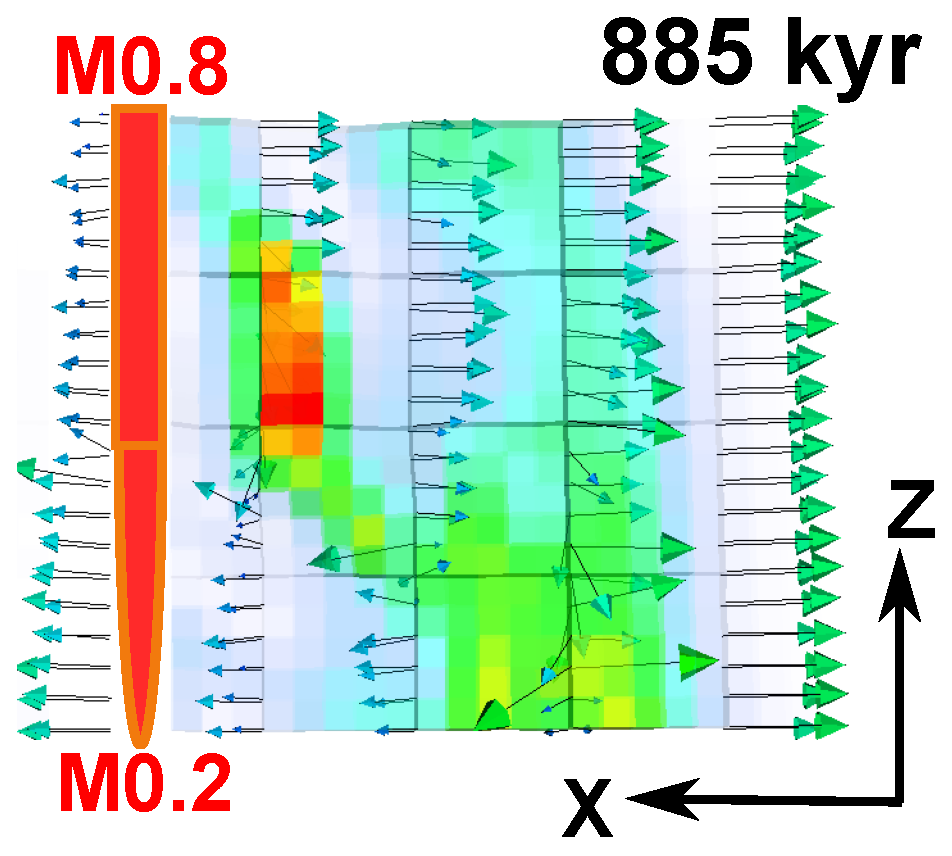
\includegraphics[width=0.5\textwidth]{./Figures/fig_Results_1_velocity_field.eps}
  \caption[Bird's-eye view of velocity field with plastic strain ploted with opacity linearly proportional to its value.]{Bird's-eye view of velocity field with plastic strain ploted with opacity linearly proportional to its value. (color scale is the same as Figure~\ref{fig_Results1_1}.a))}
 \label{fig_Results_1_velocity_field}
\end{figure}

\begin{figure}[h]
\noindent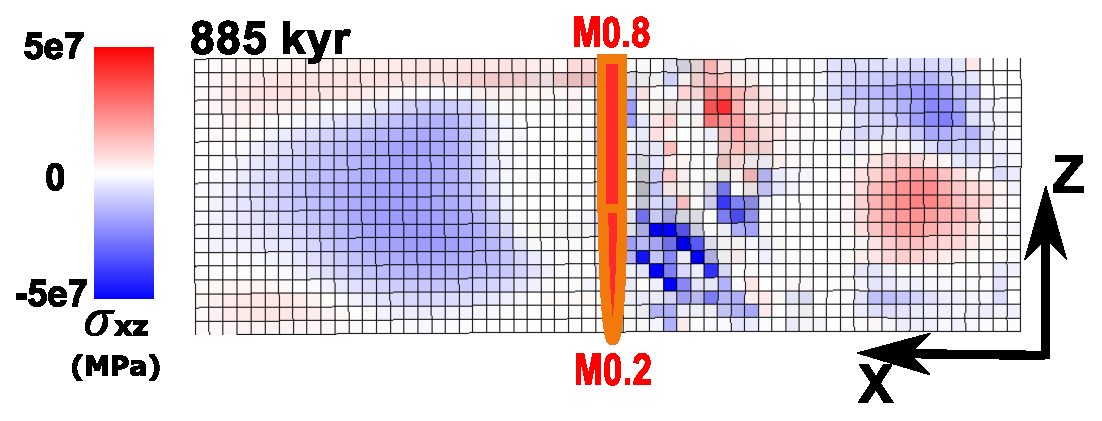
\includegraphics[width=0.8\textwidth]{./Figures/fig_Results_1_Sxz.eps}
   \caption{Bird's-eye view of $\sigma_{xz}$.}
  \label{fig_Results_1_Sxz}
\end{figure}

\begin{figure}[h]
\noindent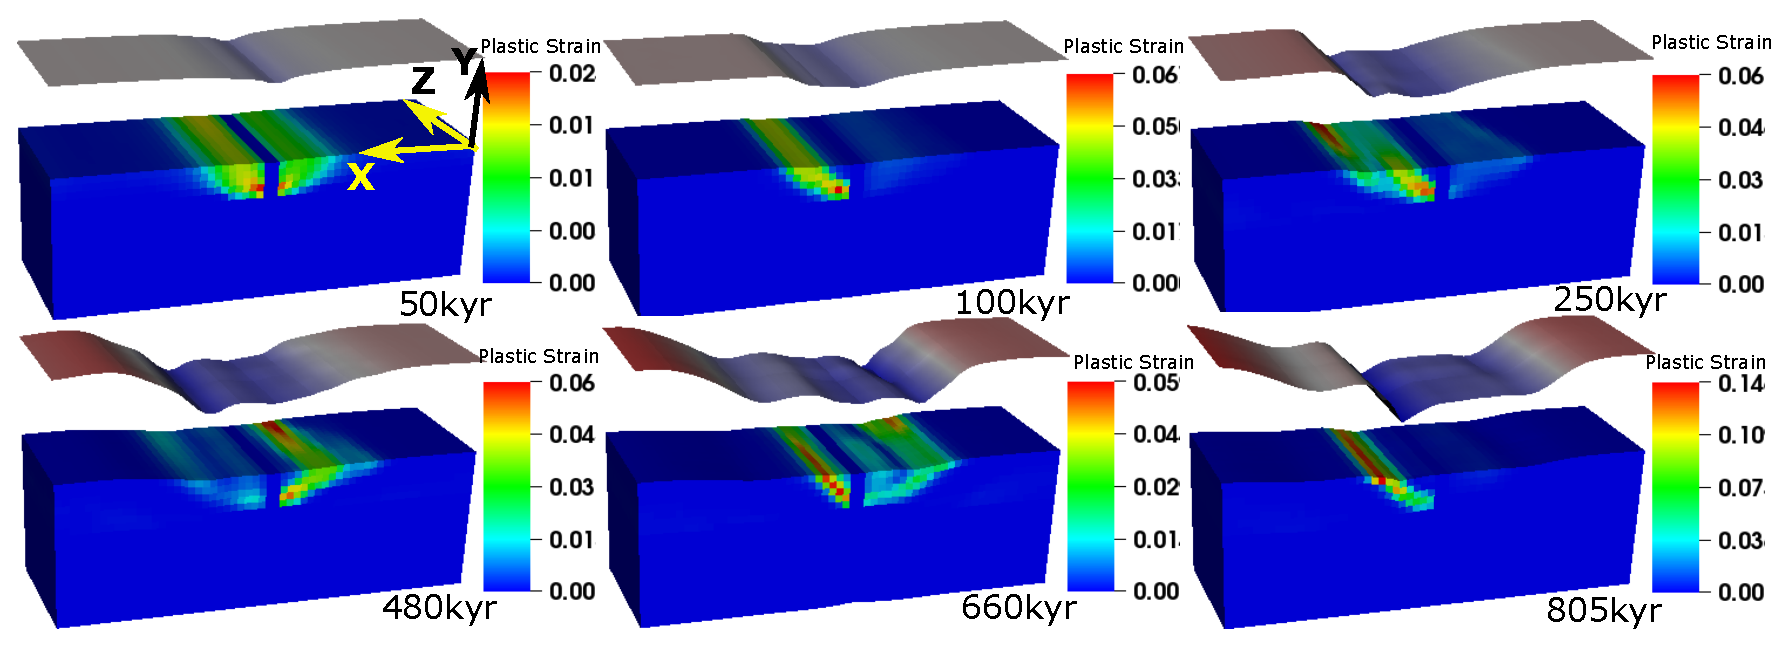
\includegraphics[width=1.0\textwidth]{./Figures/fig_Results1_3.eps}
  \caption{Evolution of plastic strain and surface topography of the model: M88ConT2 (Table~\ref{Tab1_1}). Color scale of topography is the same as Figure~\ref{fig_Results1_1}.a.}
 \label{fig_Results1_3}
\end{figure}   

\begin{figure}[h]
\noindent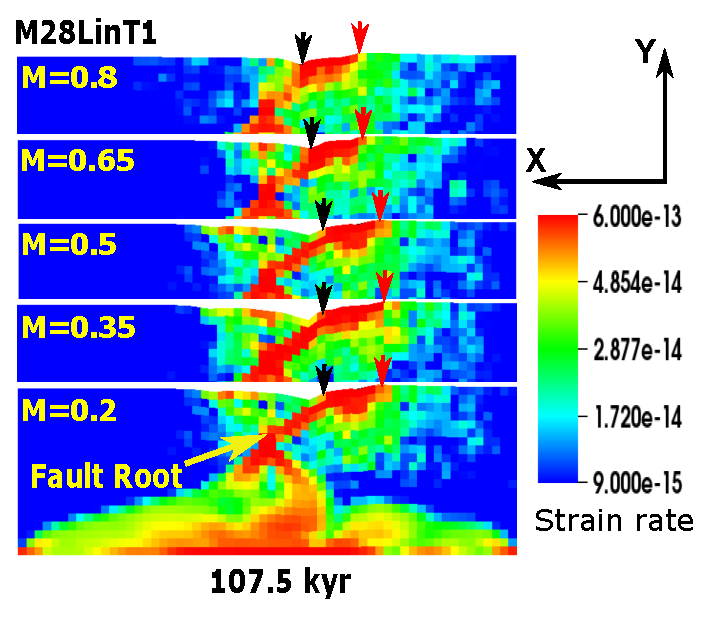
\includegraphics[width=0.6\textwidth]{./Figures/fig_Results1_2.eps}
  \caption[The second invariant of strain rates plotted on the reference model's vertical cross sections along the ridge at 107.5 kyr.]{The second invariant of strain rates plotted on the reference model's vertical cross sections along the ridge at 107.5 kyr. Terminations and breakaways are marked by black and red arrows.}
 \label{fig_Results1_2}
\end{figure}   

\begin{figure}[h]
\noindent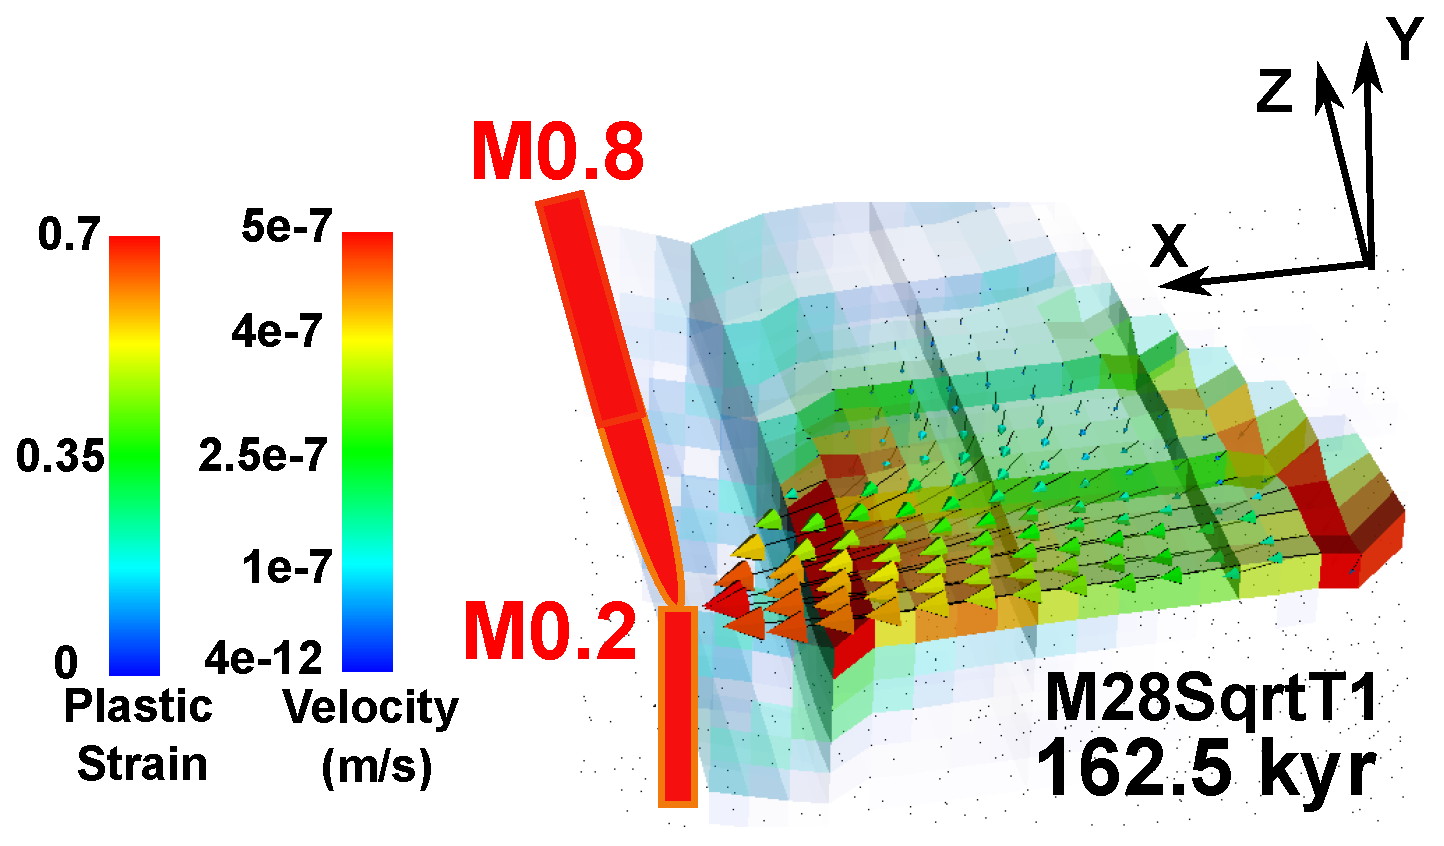
\includegraphics[width=0.6\textwidth]{./Figures/fig_Results_3_2_5_Cut-back_velocity.eps}
  \caption[Velocity of the mass wasting hanging wall.]{Velocity of the mass wasting hanging wall. Magnitudes of the velocity are shown by the colors of the arrow heads. Plastic strain is plotted with opacity linearly proportional to its value.}
 \label{fig_Results_3_2_5_Cut-back_velocity}
\end{figure}   

\begin{figure}[h]
\noindent\includegraphics[width=0.8\textwidth]{./Figures/fig_Results4_4_sqrt_cut_back_with_time_1.eps}
  \caption{Plastic strain, topography and stresses evolution for M28SqrtT1.}
 \label{fig_Results4_4}
\end{figure}  

\begin{figure}[h]
\noindent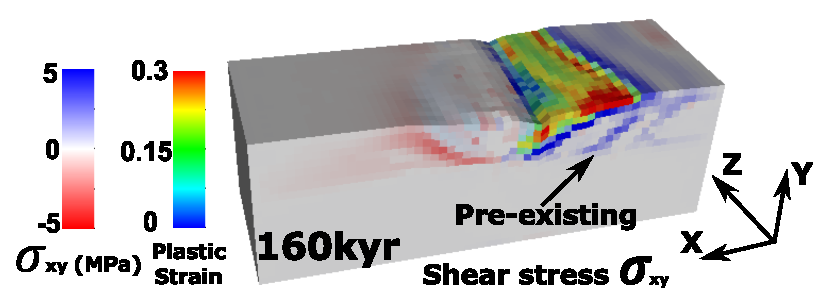
\includegraphics[width=0.6\textwidth]{./Figures/fig_Results4_5_sqrt_cut_back_pre_accummulated_shear_zone.eps}
  \caption[The weak detachment fault tip reaches the pre-existing shear stress.]{The weak detachment fault tip reaches the pre-existing shear stress. Plastic strain is plotted with opacity linearly proportional to its value.}
 \label{fig_Results4_5}
\end{figure}   

\begin{figure}[h]
\noindent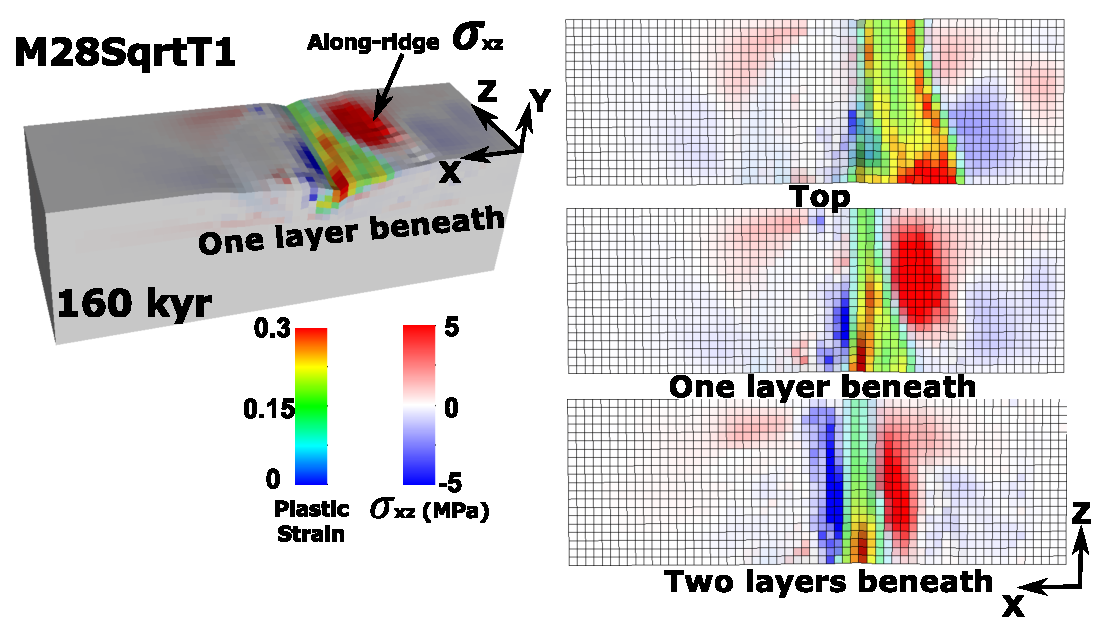
\includegraphics[width=1.0\textwidth]{./Figures/fig_Results_3_2_5_sqrt_cut_back_Sxz_beneath.eps}
  \caption[Along ridge axis $\sigma_{xz}$.]{Along ridge axis $\sigma_{xz}$ (bird's-eye view of three layers of model domain) (positive(red) means clockwise). Plastic strain is plotted with opacity linearly proportional to its value.}
 \label{fig_Results_3_2_5_sqrt_cut_back_Sxz_beneath}
\end{figure}

\begin{figure}[h]
\noindent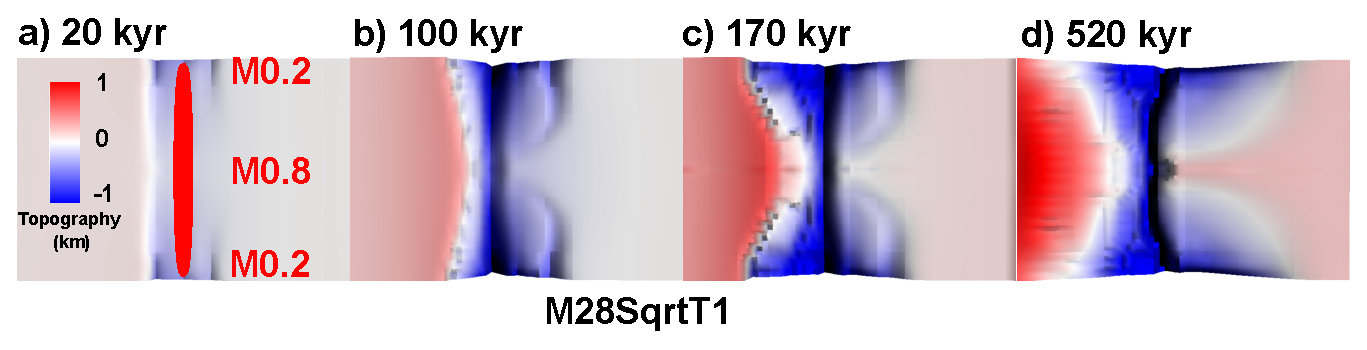
\includegraphics[width=1.0\textwidth]{./Figures/fig_Results_3_2_hourglass_evolution.eps}
  \caption[Bird's-eye view of the evolution of the hourglass-shaped median valley.]{Bird's-eye view of the evolution of the hourglass-shaped median valley. It is generated by attaching the topography of the M28SqrtT1 model to its mirror image by assumming symmetrical M variation (0.2 to 0.8 to 0.2). }
 \label{fig_Results_3_2_hourglass_evolution}
\end{figure}

\begin{figure}[h]
\noindent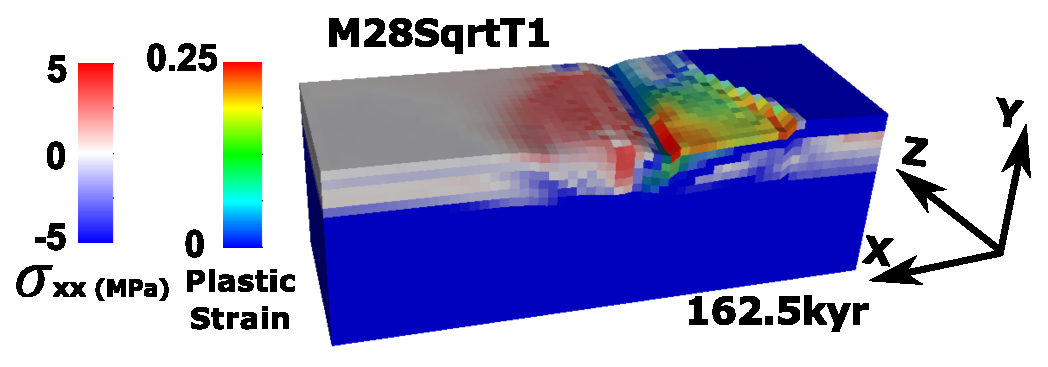
\includegraphics[width=0.6\textwidth]{./Figures/fig_Results4_7_sqrt_cut_back_conjugate_Sxx.eps}
  \caption{Higher $\sigma_{xx}$ shows inside the median valley on the positive $x$-axis direction of the ridge axis. }
 \label{fig_Results4_7}
\end{figure}

\begin{figure}[h]
\noindent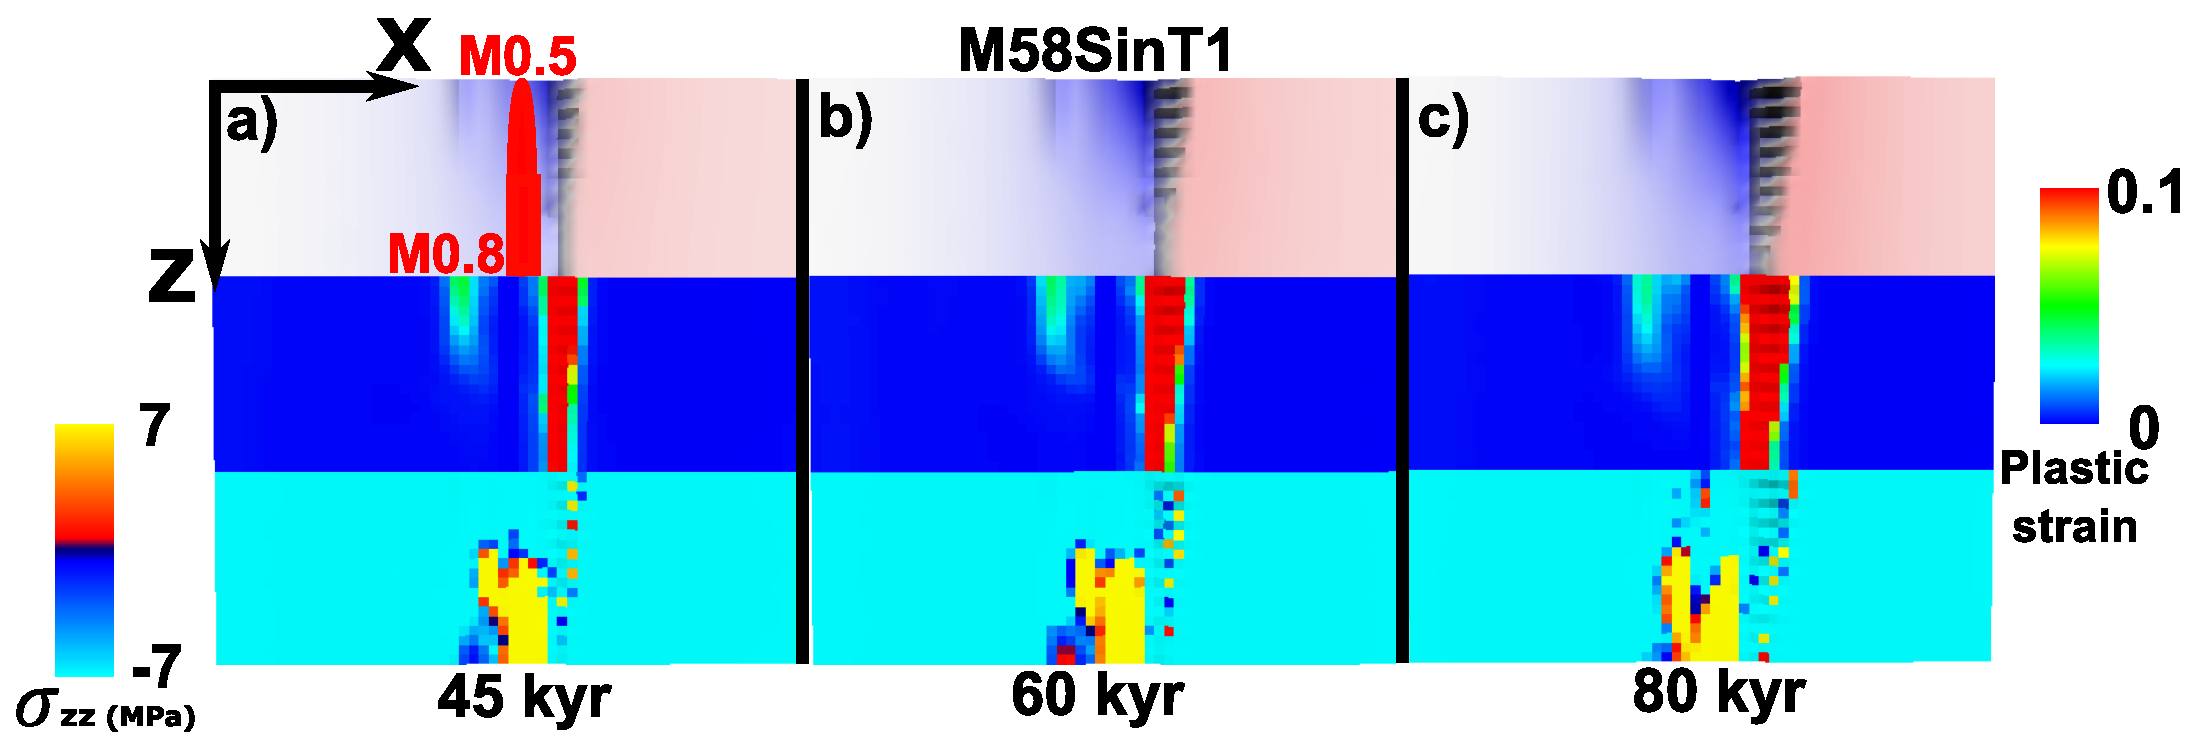
\includegraphics[width=1.0\textwidth]{./Figures/fig_Results_3_2_6_corrugations_evolution.eps}
  \caption[Bird's-eye view of the evolution of the corrugations.]{Bird's-eye view of the evolution of the corrugations. Color scales for the topography is the same as Figure~\ref{fig_Results1_1}.}
 \label{fig_Results_3_2_6_corrugations_evolution}
\end{figure}

\begin{figure}[h]
\noindent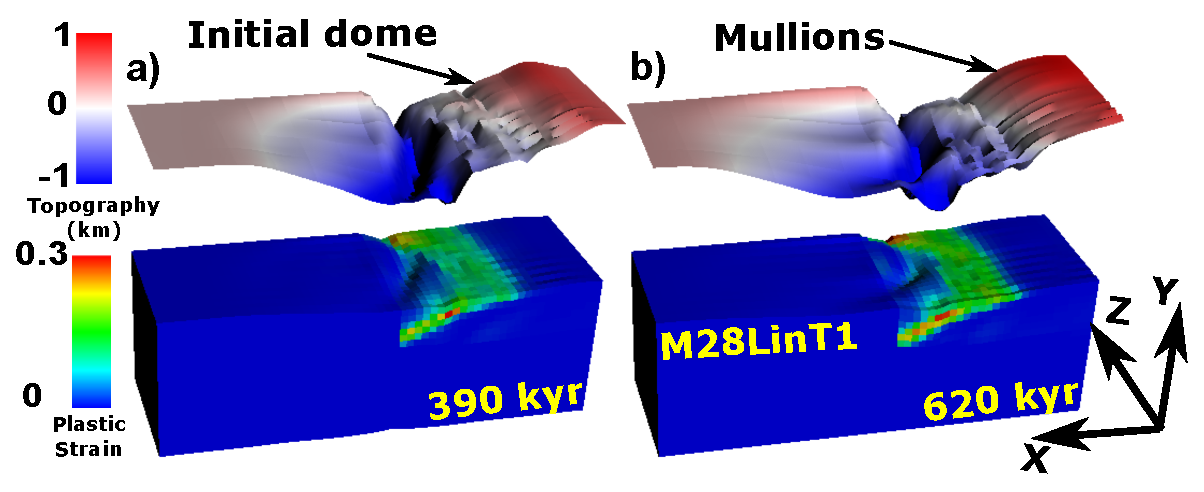
\includegraphics[width=1.0\textwidth]{./Figures/fig_Results_3_2_6_mullion_evolution.eps}
  \caption{Evolution of mullion structures.}
 \label{fig_Results_3_2_6_mullion_evolution}
\end{figure}

\begin{figure}[h]
\noindent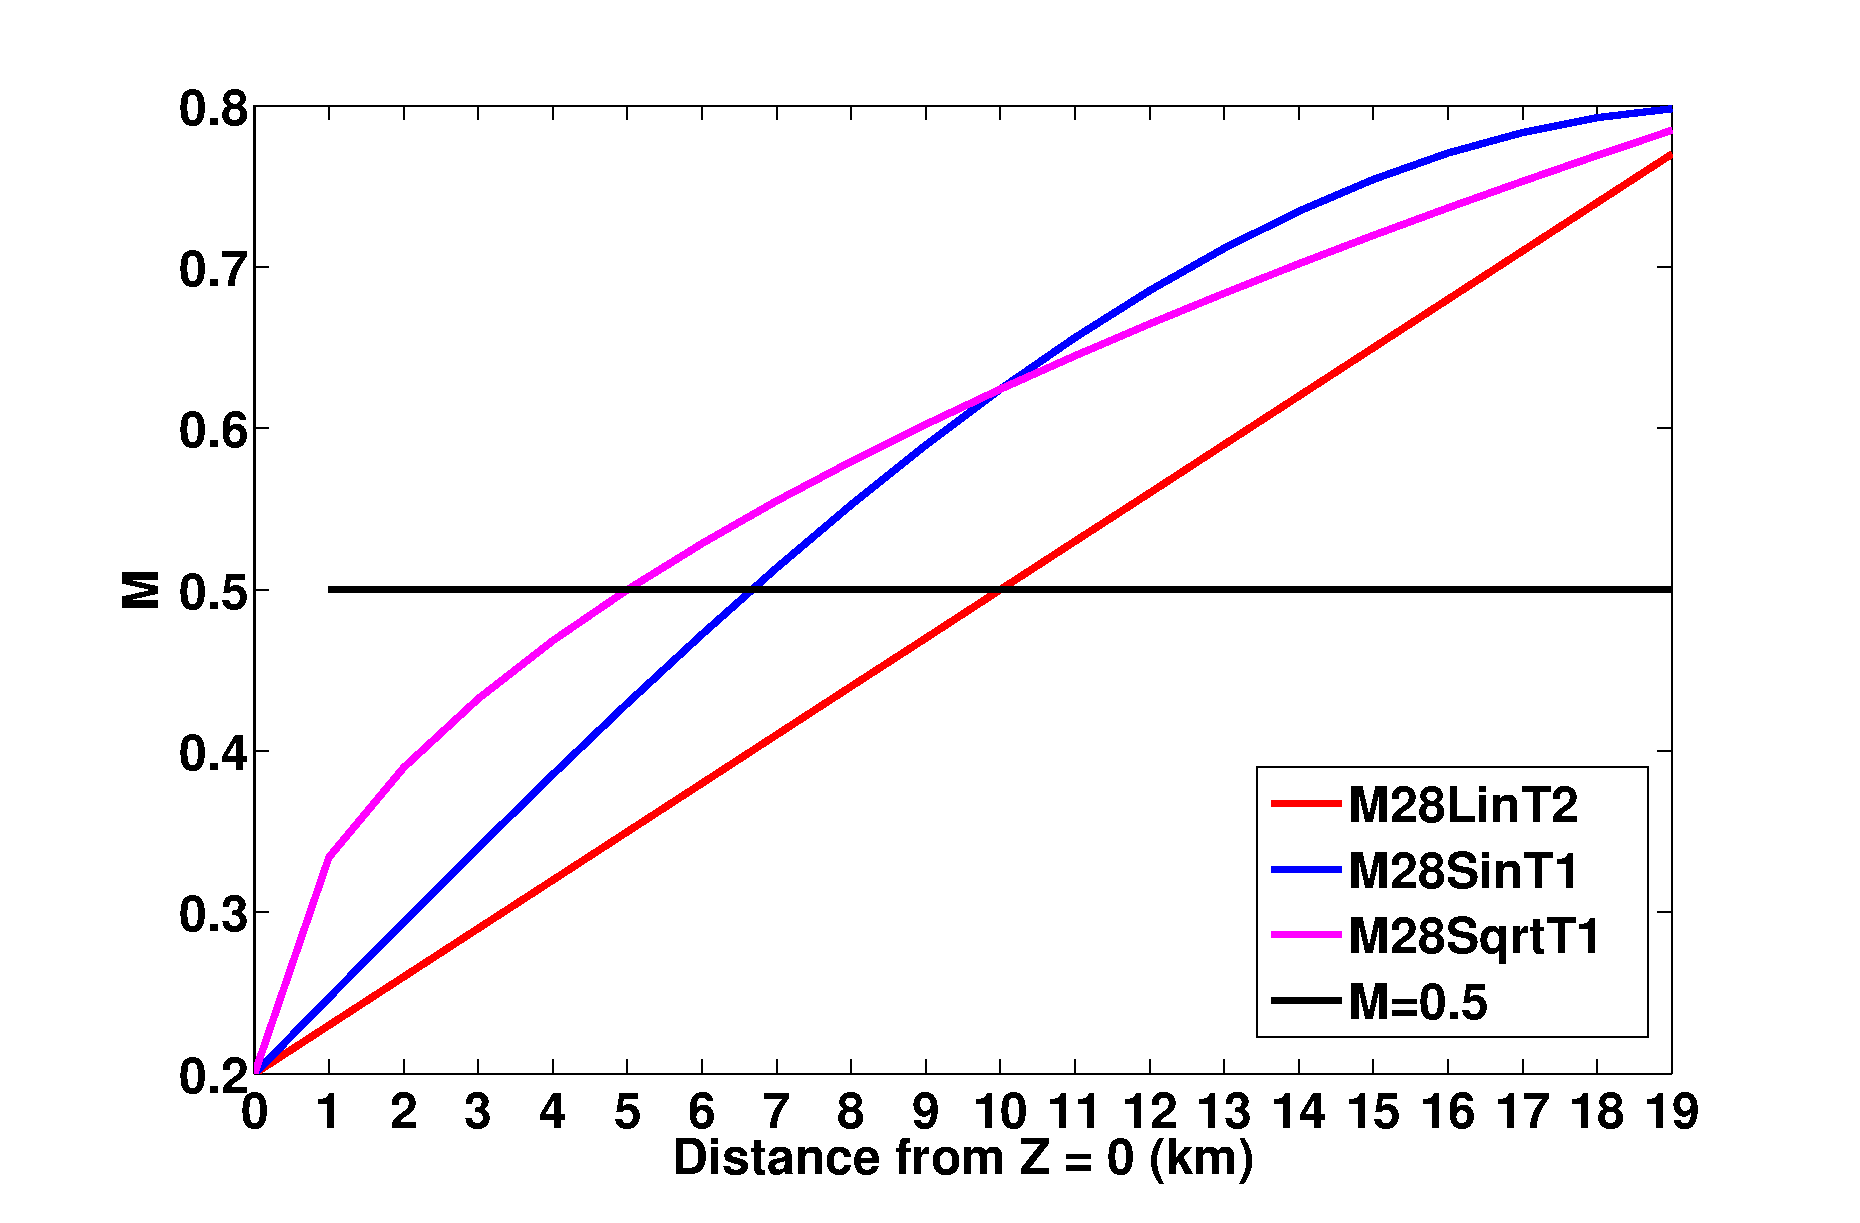
\includegraphics[width=0.8\textwidth]{./Figures/fig_Results_3_3_M_variation.eps}
  \caption[Three functional forms of M variation.]{Three functional forms of M variation. M begins to exceed the M $=$ 0.5 black line at Z=10 km, 7 km, 5 km for M28LinT1, M28SinT1 and M28SqrtT1 respectively.}
 \label{fig_Results3_1}
\end{figure}   

\begin{figure}[h]
\noindent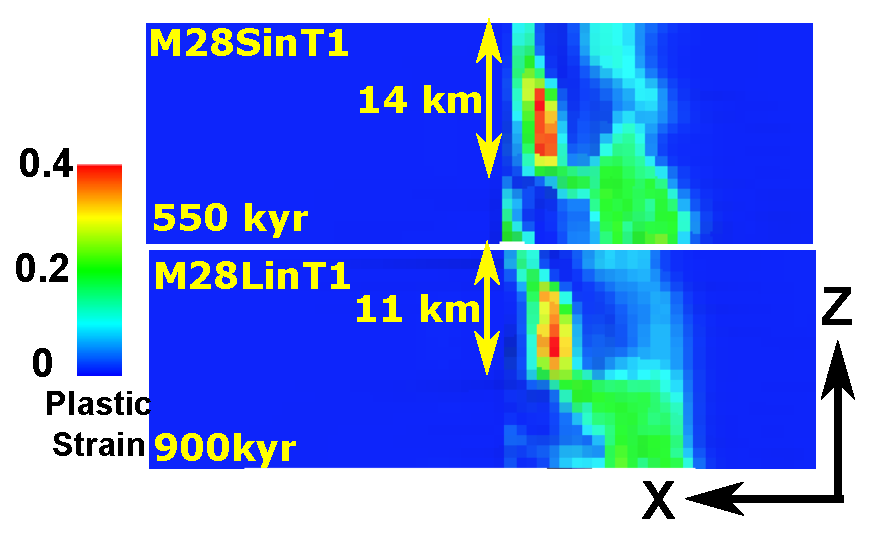
\includegraphics[width=0.6\textwidth]{./Figures/fig_Results4_2_secondary_fault_length_comparison1.eps}
  \caption{Bird's-eye view for comparing the length and timing of inward fault jump.}
 \label{fig_Results4_2}
\end{figure}   

\begin{figure}[h]
\noindent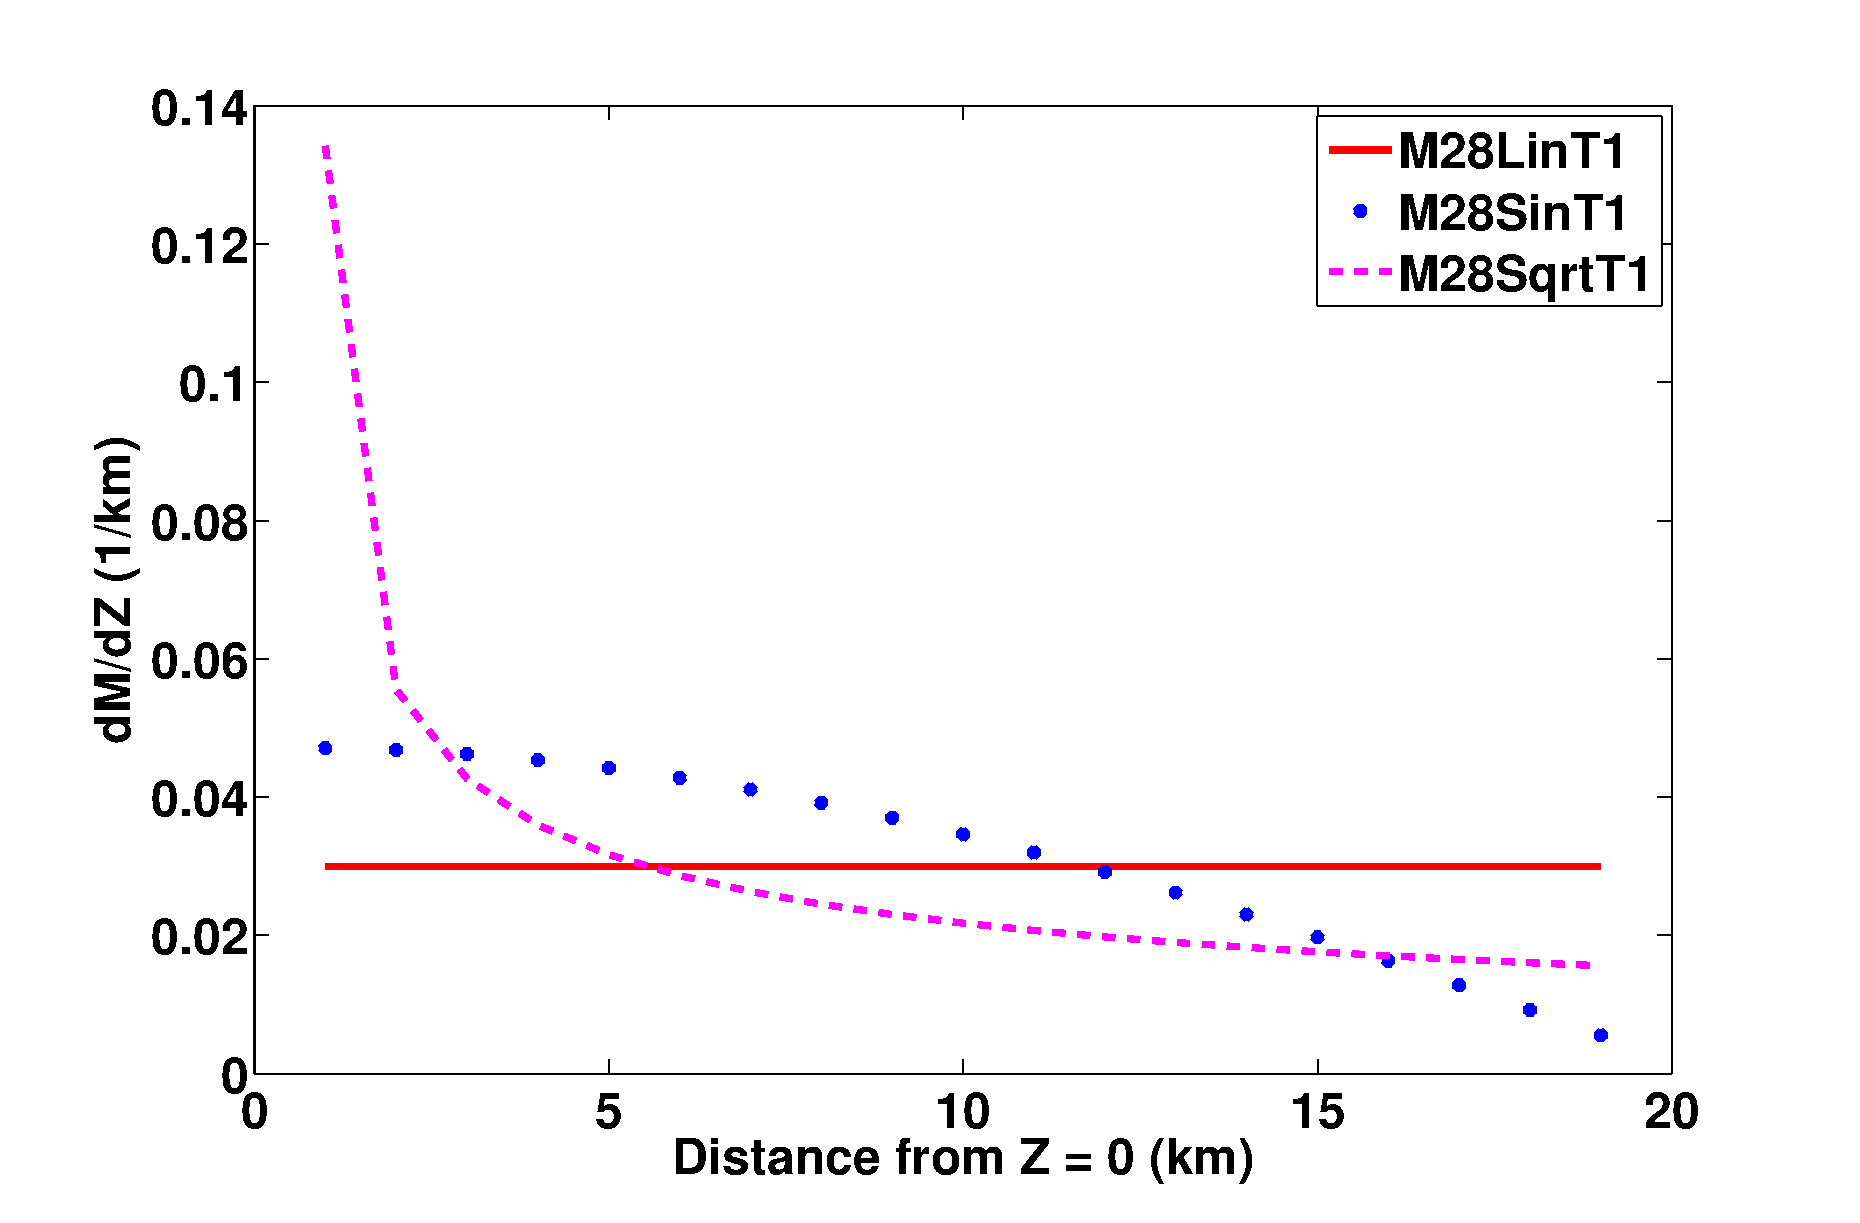
\includegraphics[width=0.8\textwidth]{./Figures/fig_Results_3_3_1_M_type_plot_dM_dZ.eps}
  \caption{$\partial M/ \partial Z$ comparision.}
 \label{fig_Results_3_3_1_M_type_plot_dM_dZ}
\end{figure}  

\begin{figure}[h]
\noindent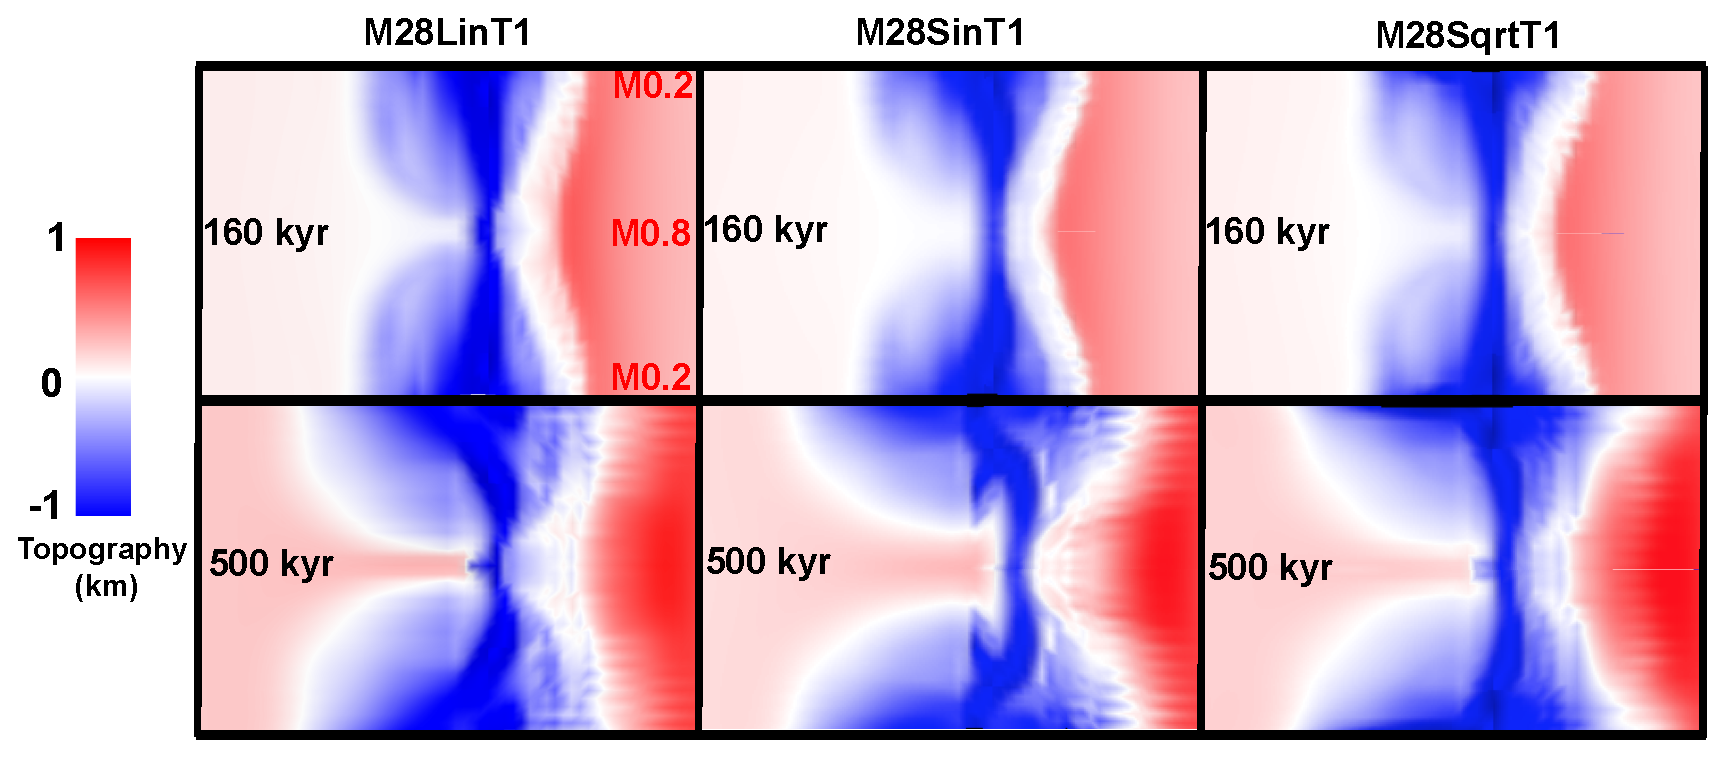
\includegraphics[width=1.0\textwidth]{./Figures/fig_Results_3_3_1_hourglass.eps}
  \caption[Bird's-eye view of the topograpy.]{Bird's-eye view of the topograpy. (Original and mirror images are put together assumming symmetrical M variation.) }
 \label{fig_Results_3_3_1_hourglass}
\end{figure} 

\begin{figure}[h]
\noindent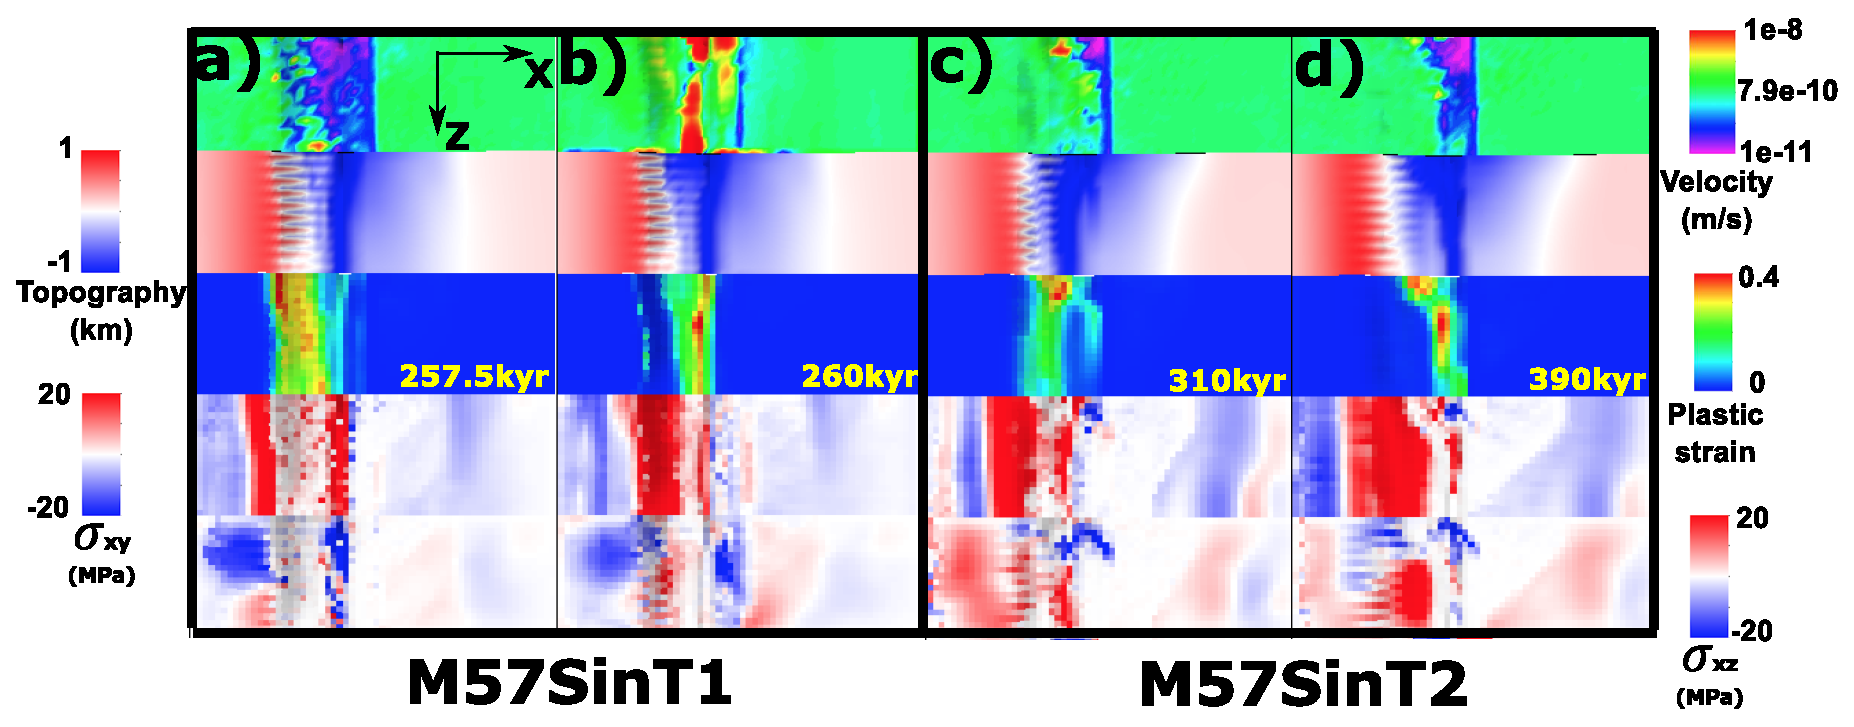
\includegraphics[width=1.0\textwidth]{./Figures/fig_Results_Weakening_2_M57SinT1VST2_CutbackVSsecondaryFault.eps}
 \caption{Bird's-eye view of M57SinT2 versus M57SinT1 (Table~\ref{Tab1_1}).}
\label{fig_Results_Weakenging_2}
\end{figure}

\begin{figure}[h]
\noindent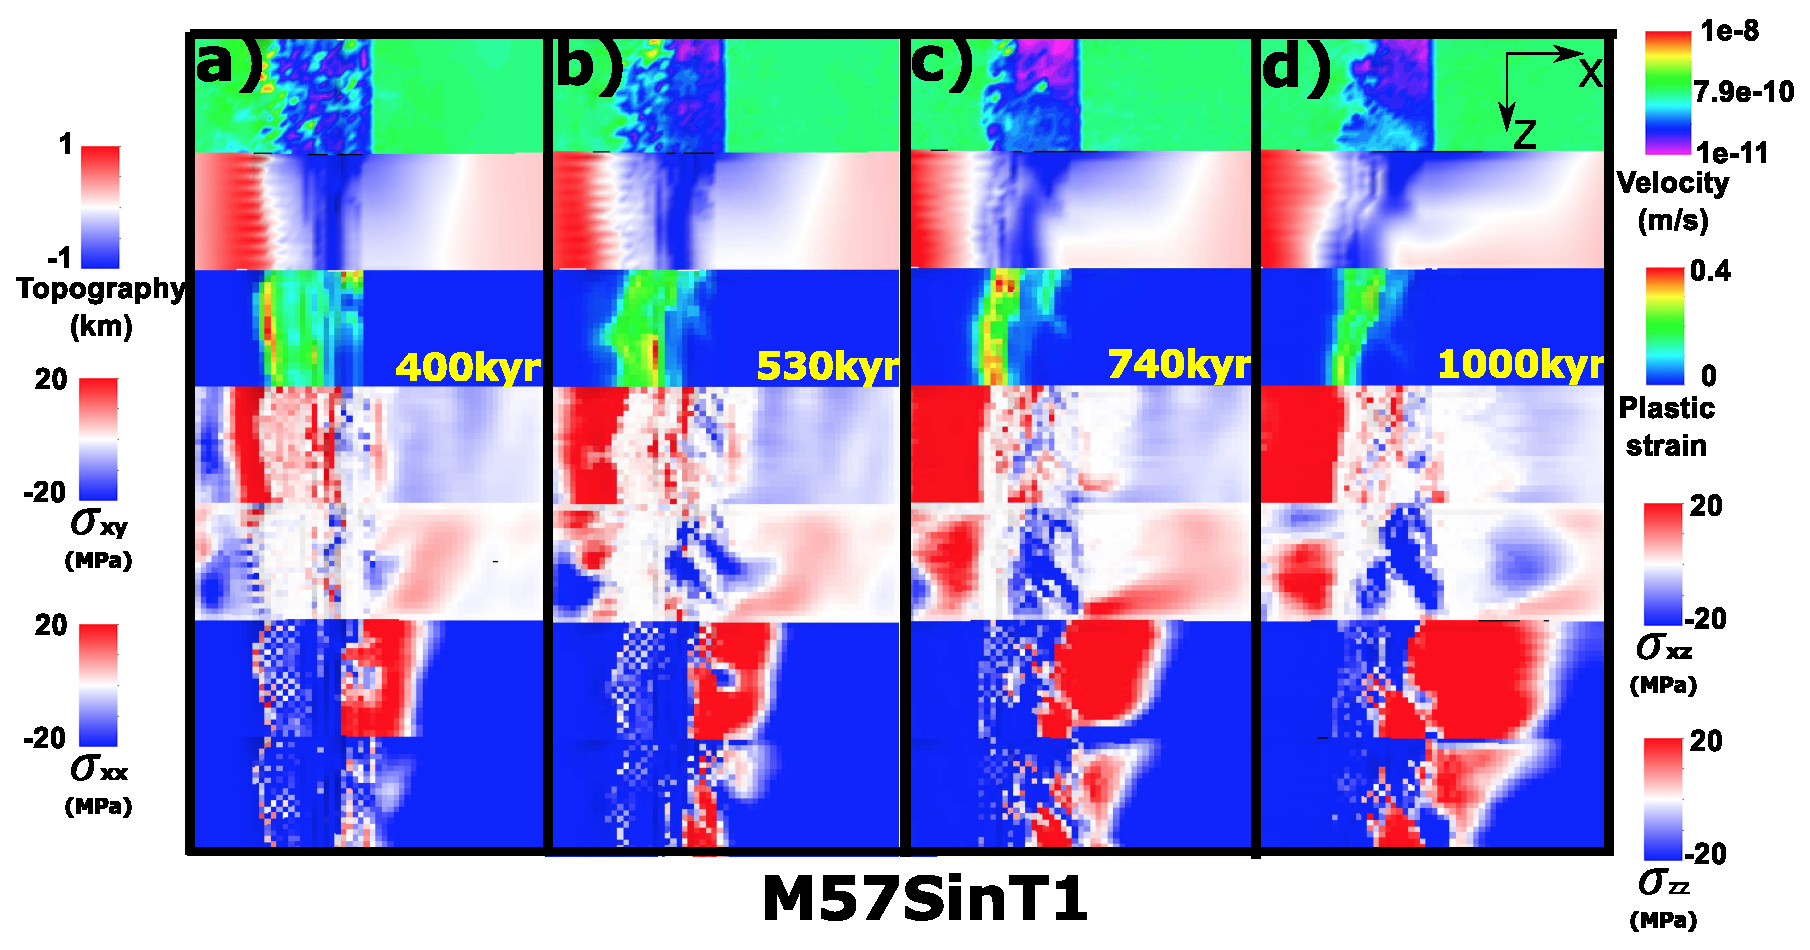
\includegraphics[width=1.0\textwidth]{./Figures/fig_Results_Weakening_3_M57SinT1_time_evolution.eps}
 \caption{Bird's-eye view of faulting and stresses evolution of M57SinT1.}
\label{fig_Results_Weakenging_3}
\end{figure}

\begin{figure}[h]
\noindent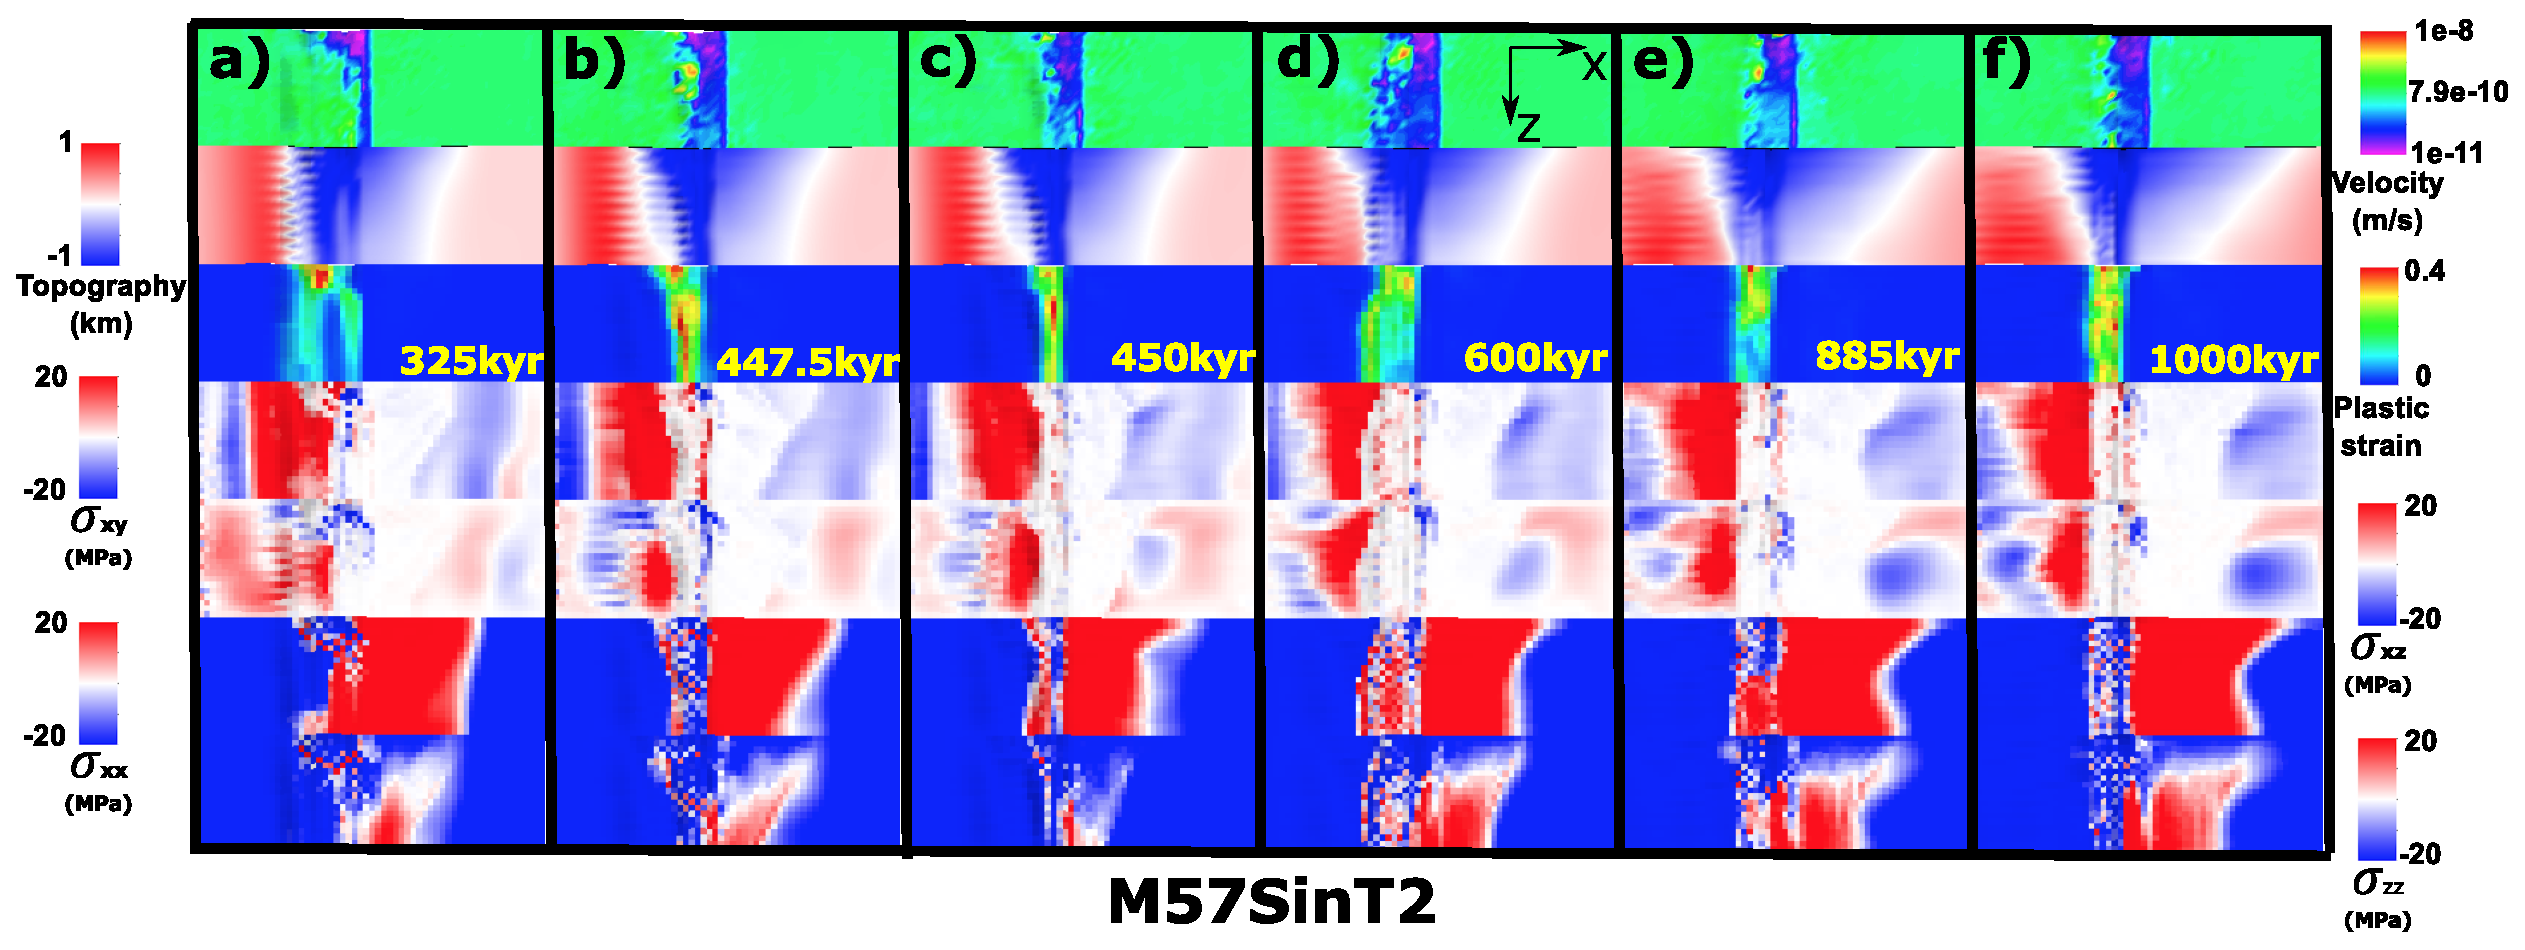
\includegraphics[width=1.0\textwidth]{./Figures/fig_Results_Weakening_4_M57SinT2_time_evolution.eps}
 \caption{Bird's-eye view of faulting and stresses evolution of M57SinT2.}
\label{fig_Results_Weakenging_4}
\end{figure}

\begin{figure}[h]
\noindent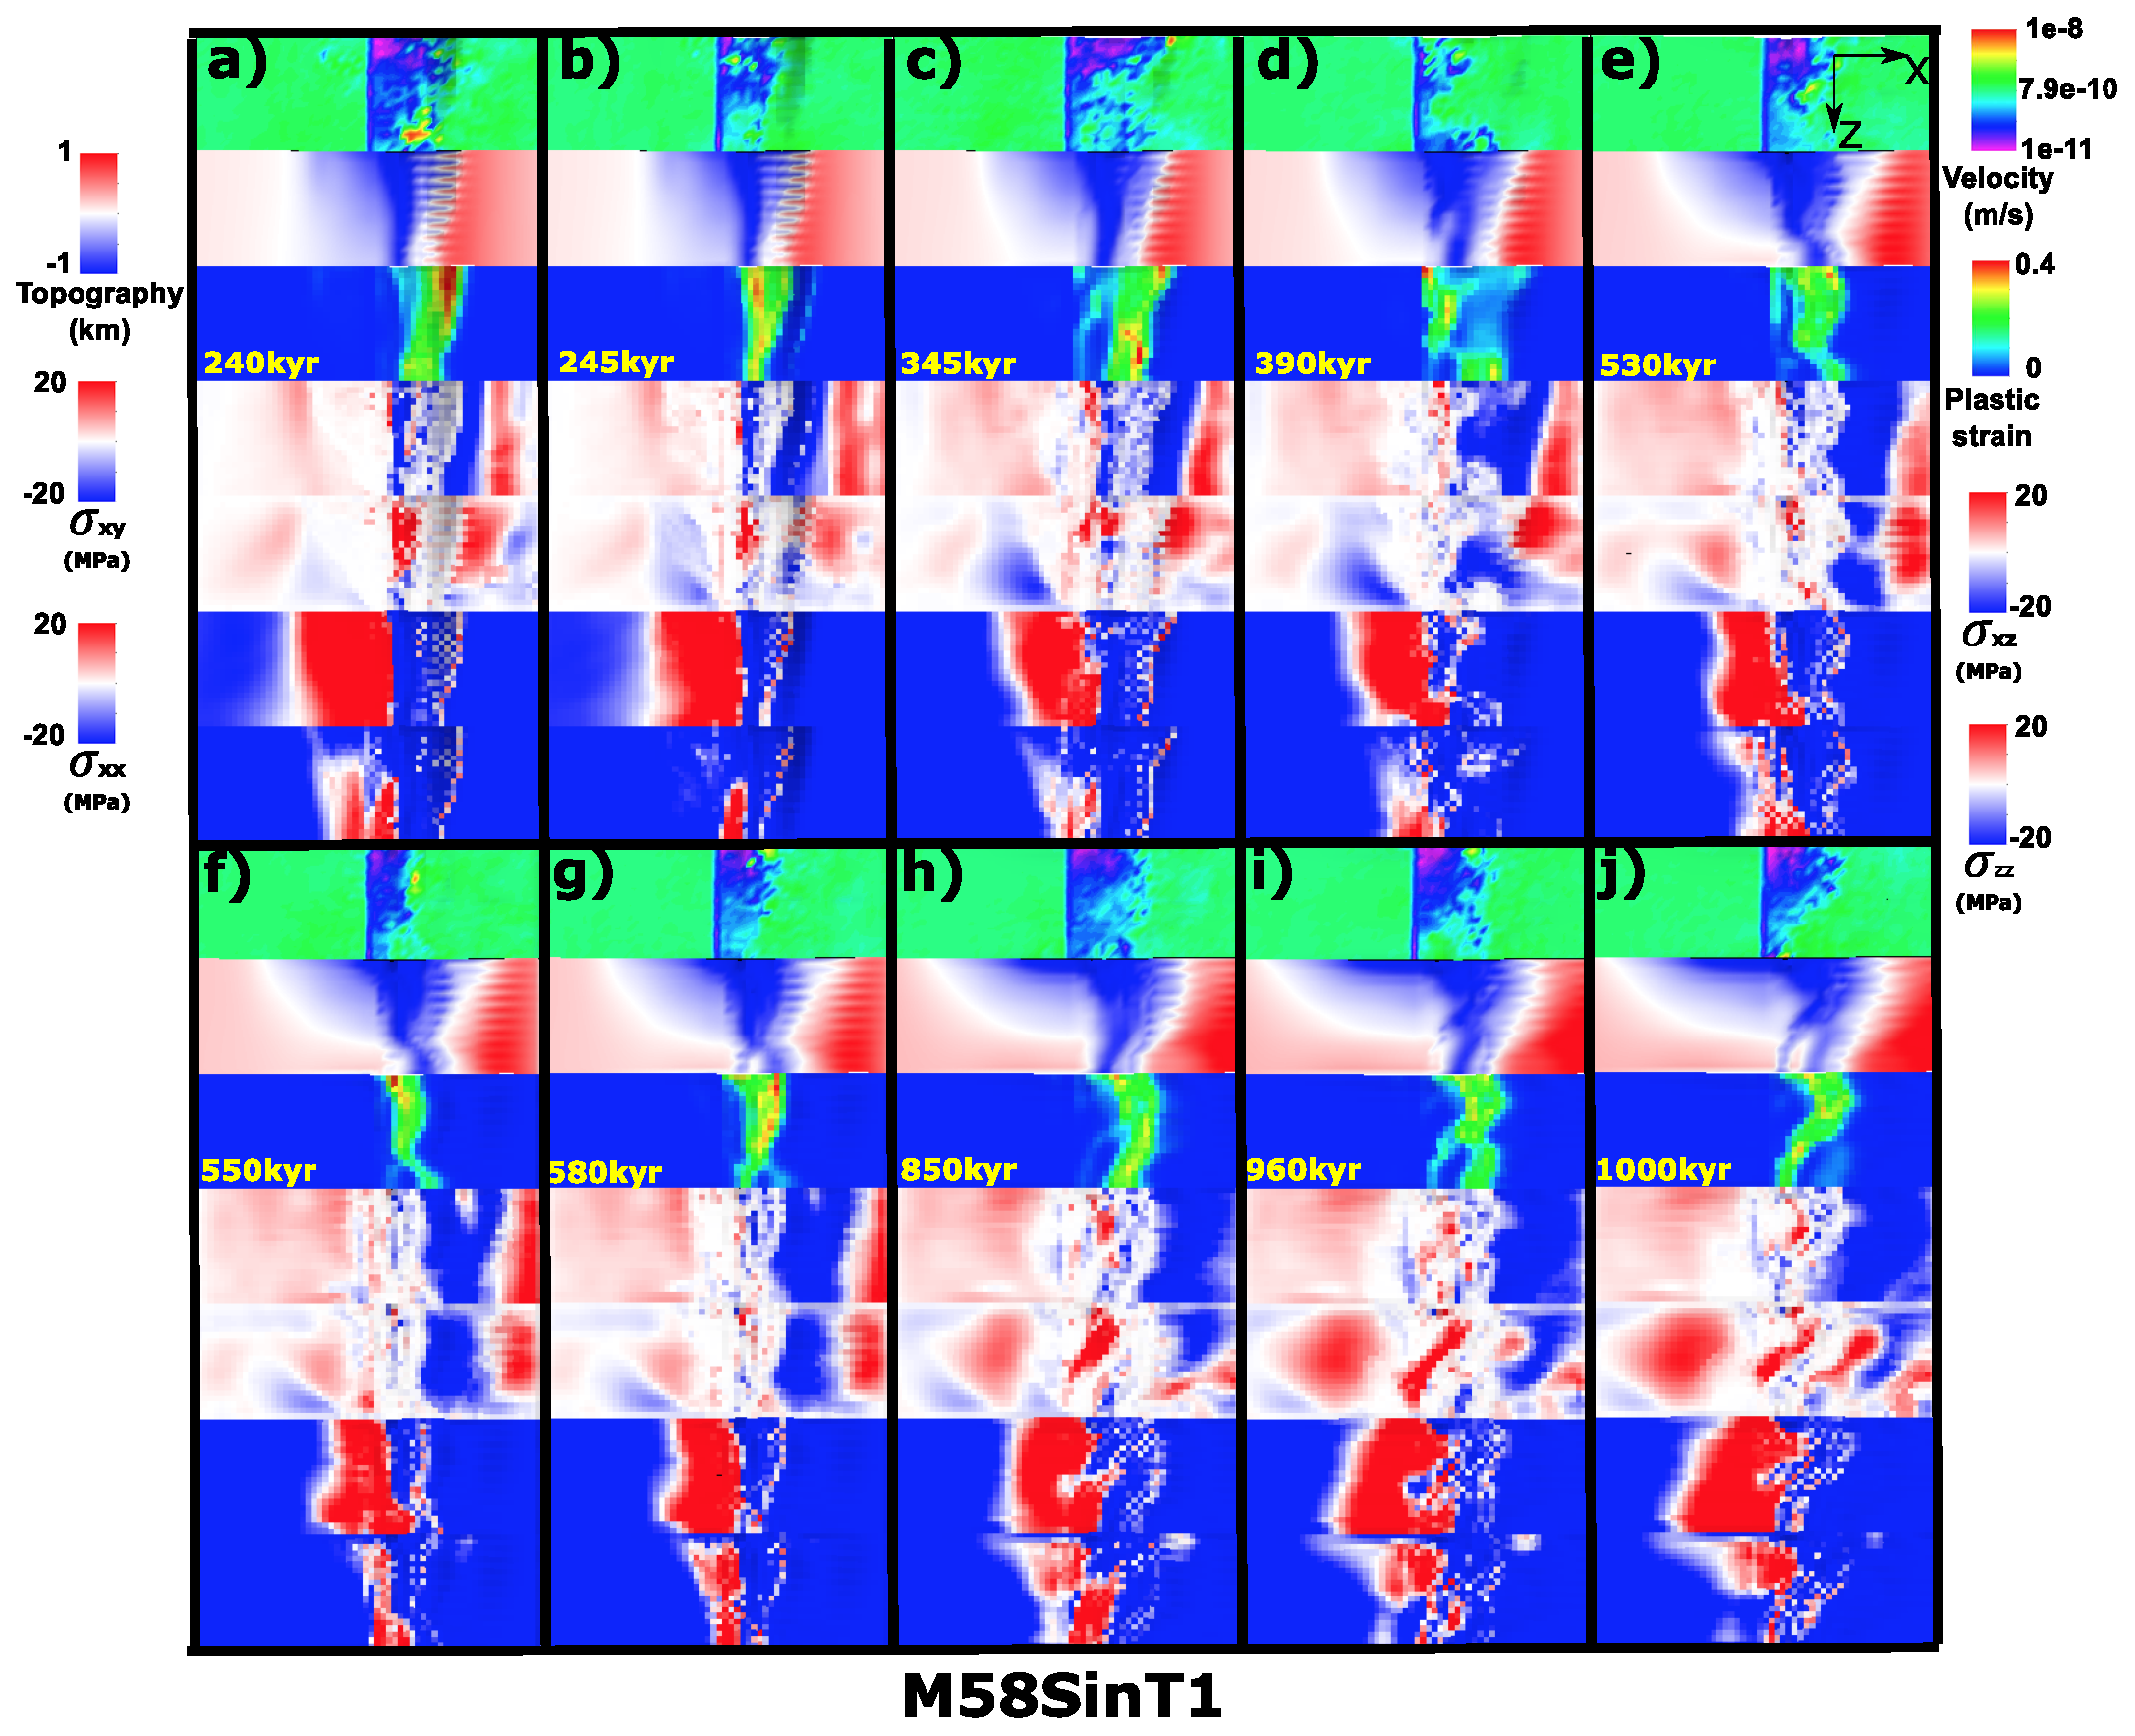
\includegraphics[width=1.0\textwidth]{./Figures/fig_Results_Weakening_5_M58SinT1_time_evolution.eps}
 \caption{Bird's-eye view of faulting and stresses evolution of M58SinT1.}
\label{fig_Results_Weakenging_5}
\end{figure}

\begin{figure}[h]
\noindent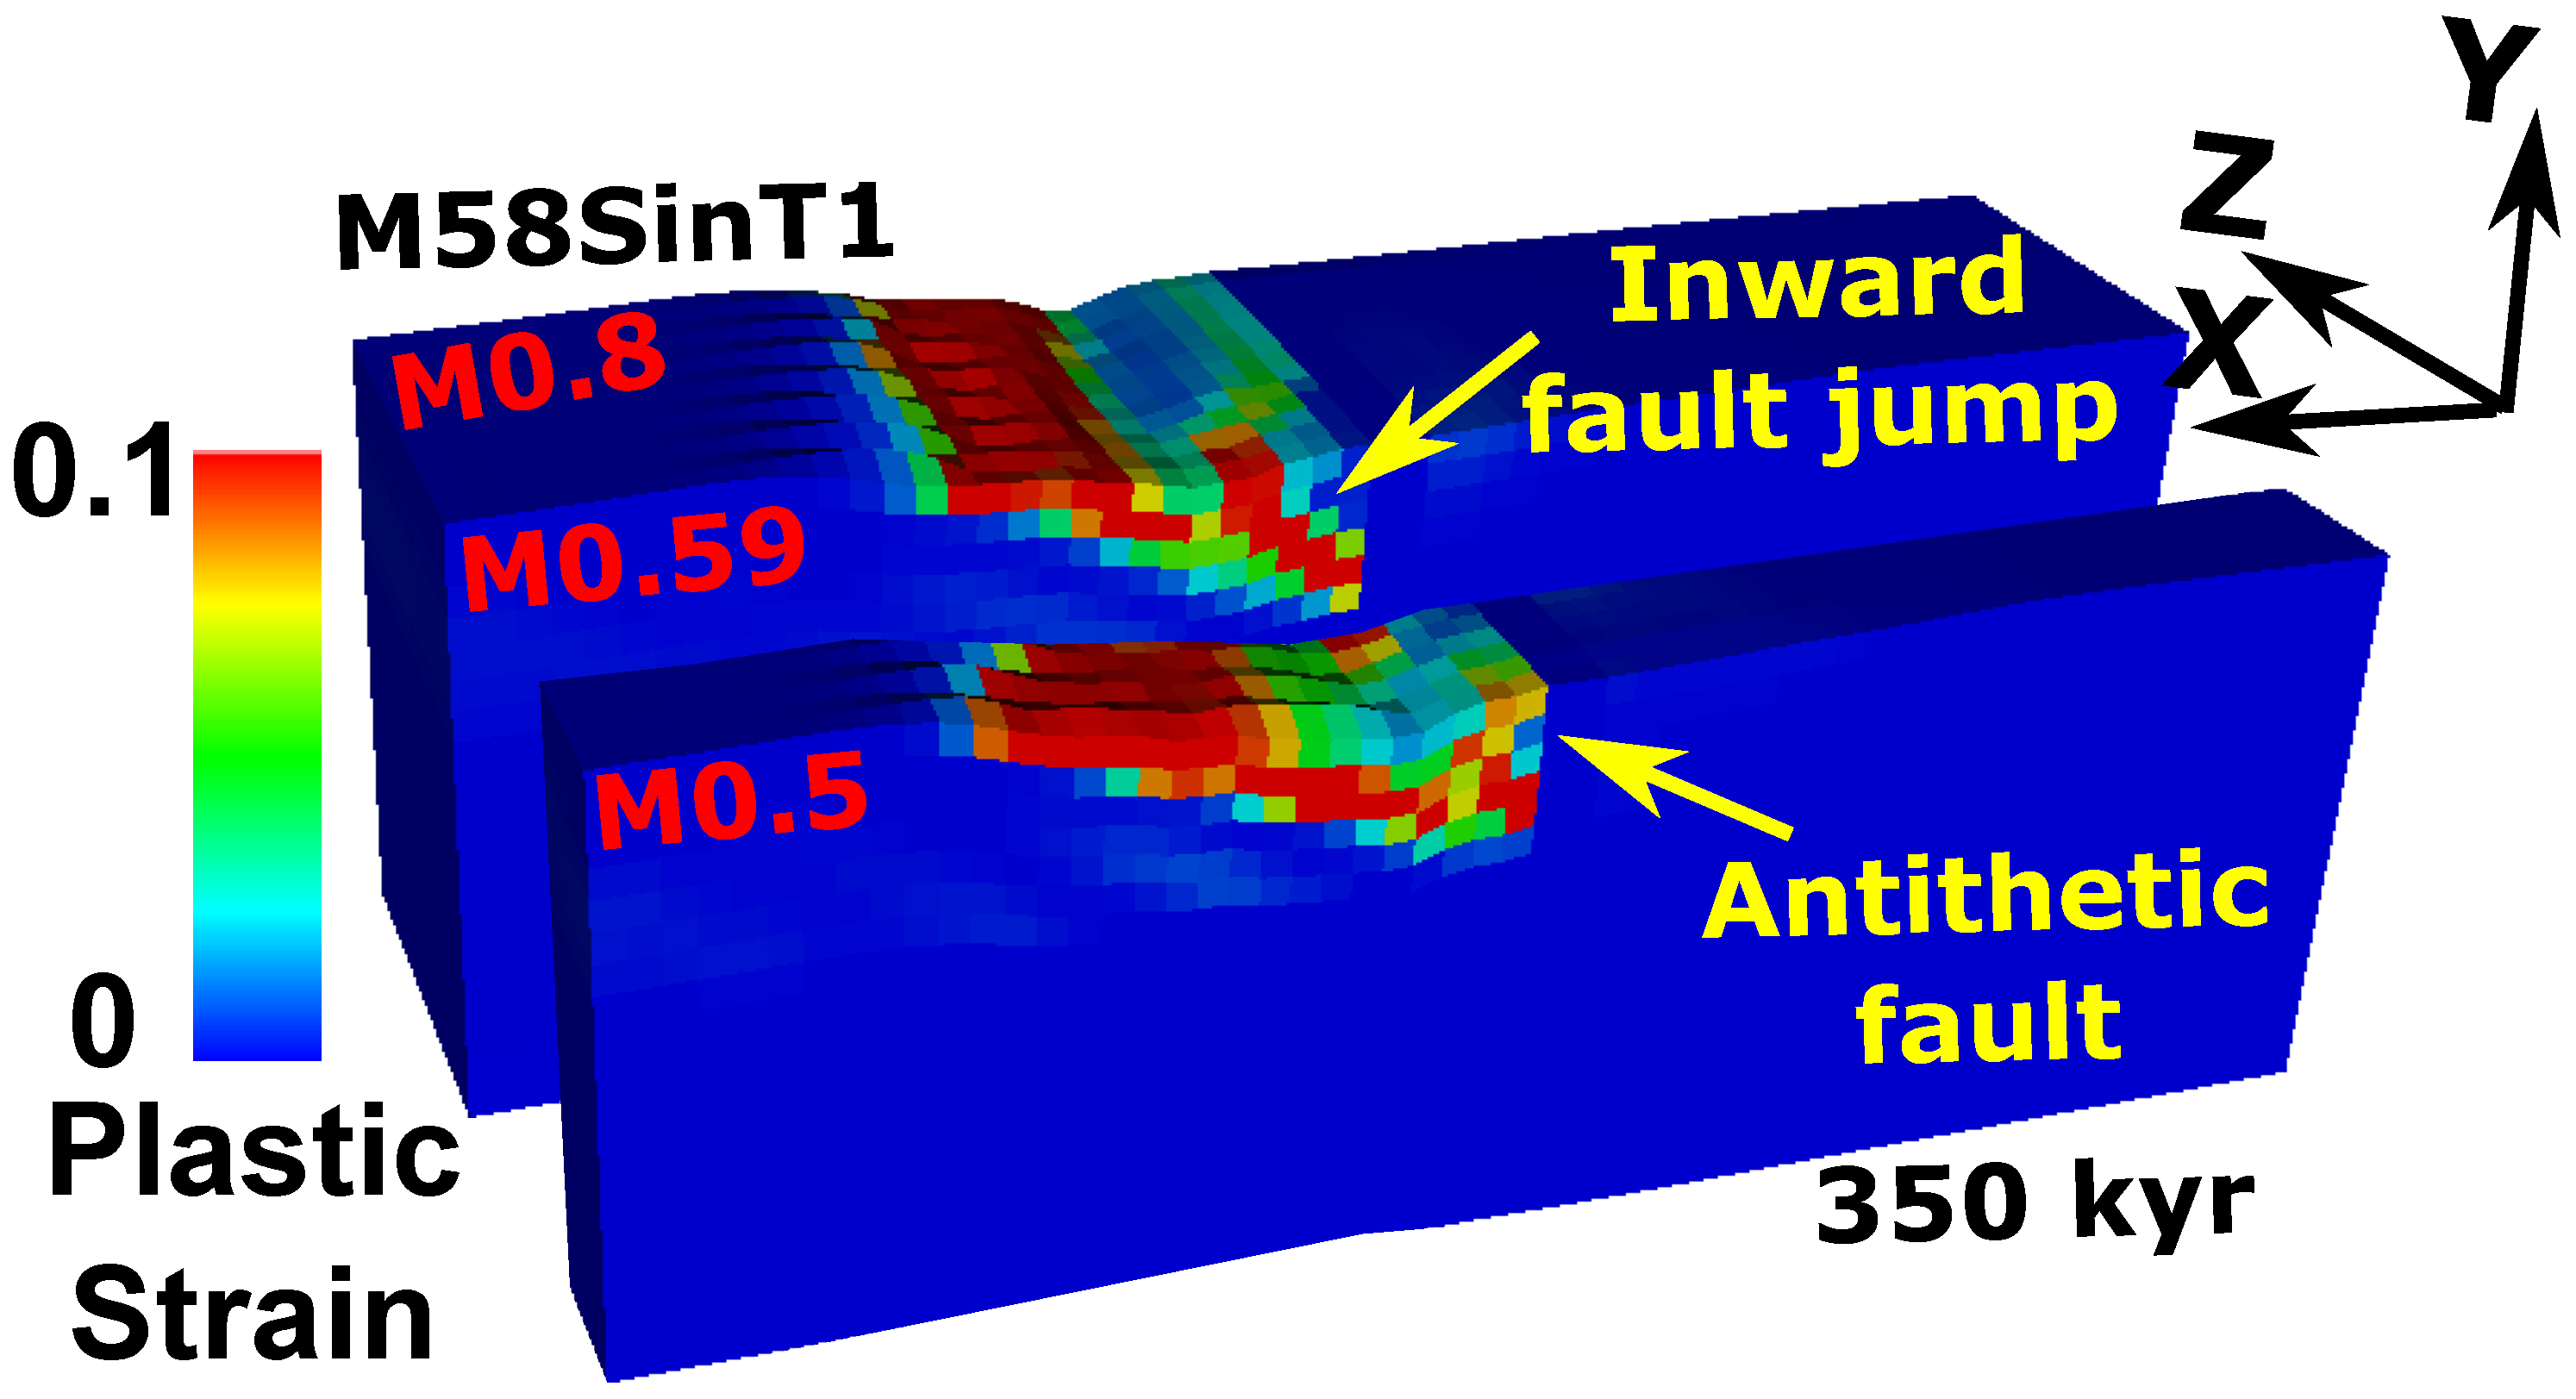
\includegraphics[width=0.6\textwidth]{./Figures/fig_Results_3_4_2_3D_Antithetic_fault.eps}
 \caption{Plastic strain for M58SinT1 at 350 kyr.}
\label{fig_Results_3_4_2_3D_Antithetic_fault}
\end{figure}

\begin{figure}[h]
\noindent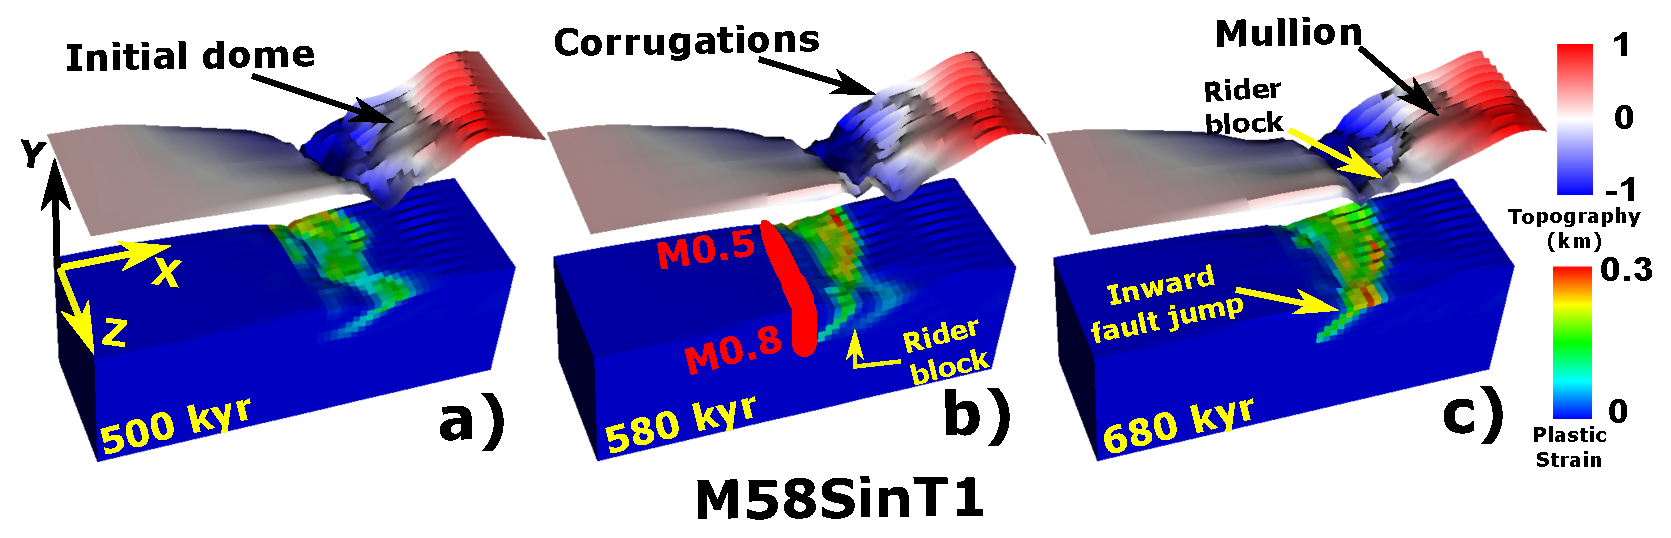
\includegraphics[width=1.0\textwidth]{./Figures/fig_Results_3_4_2_M58SinT1_mullion_riderBlock_inwardFaultJump.eps}
 \caption{Evolution of faulting and morphologies of M58SinT1.}
\label{fig_Results_3_4_2_M58SinT1_mullion_riderBlock_inwardFaultJump}
\end{figure}

\begin{figure}[h]
\noindent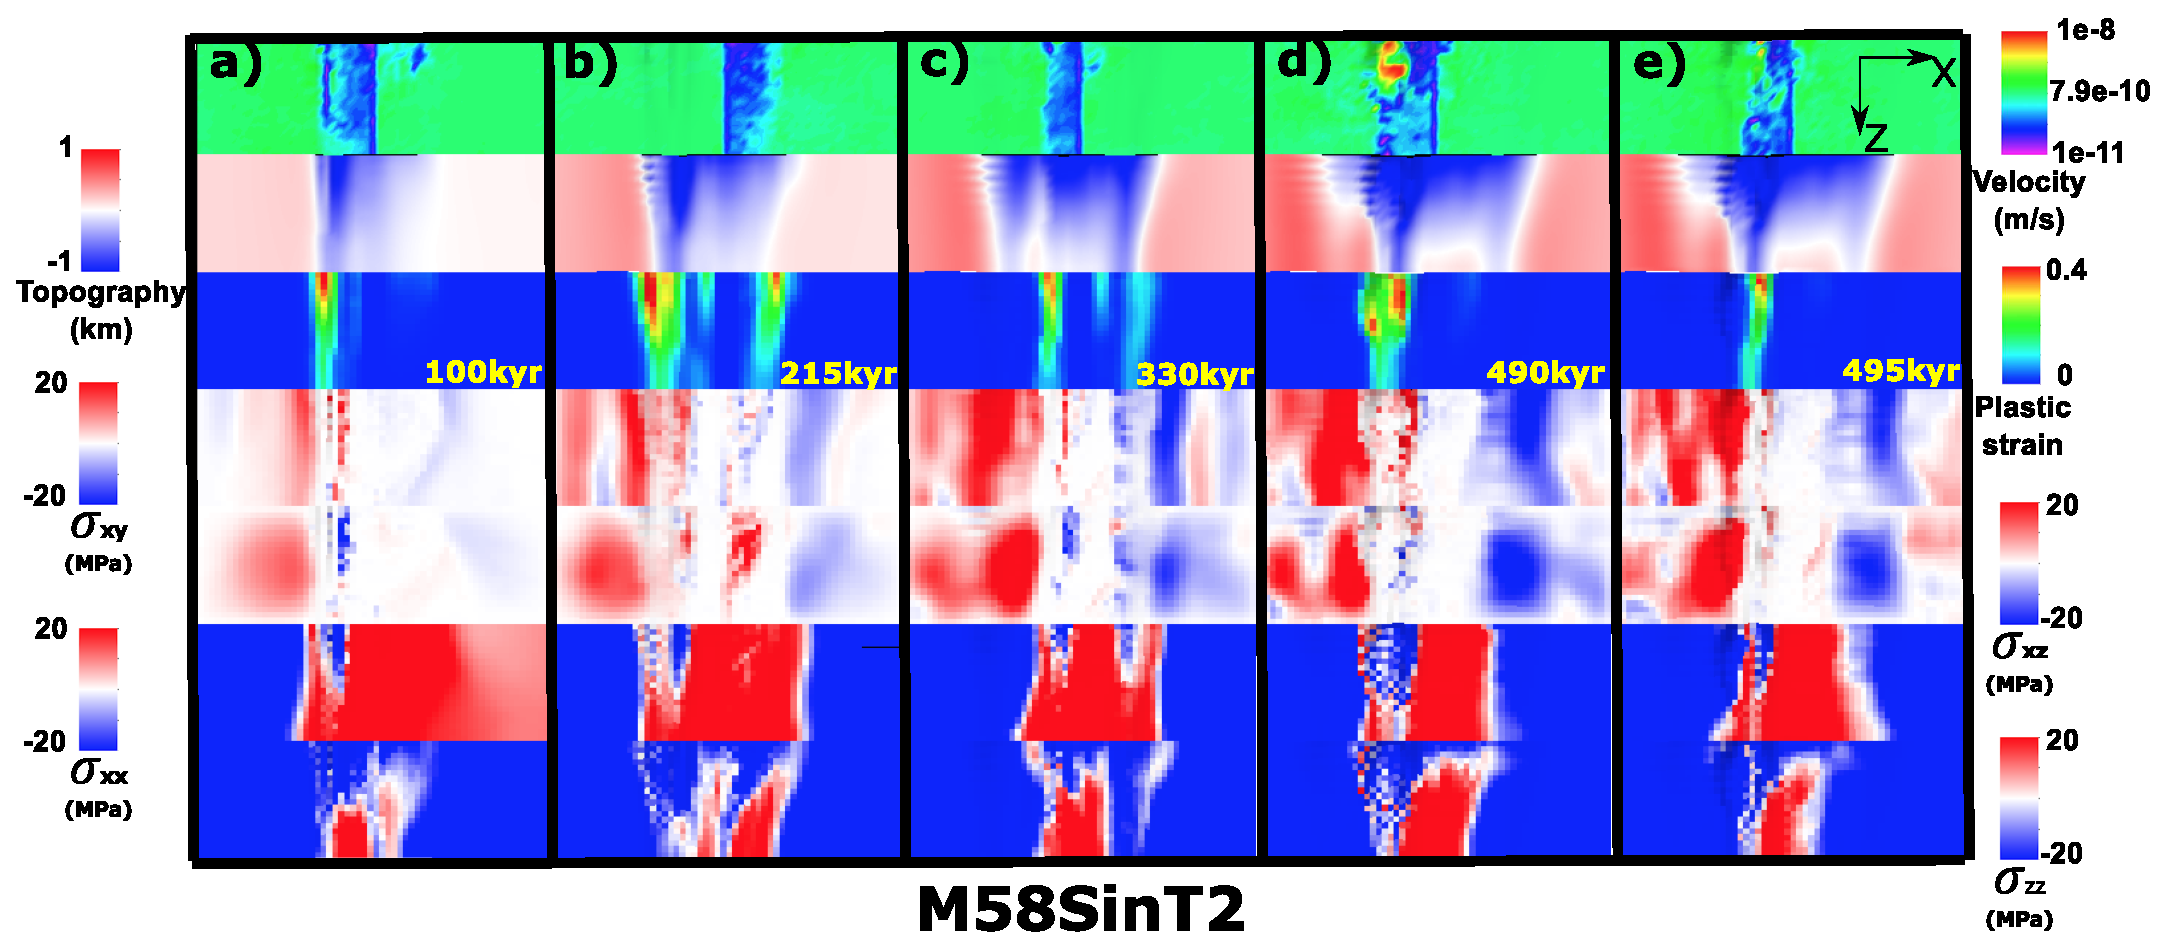
\includegraphics[width=1.0\textwidth]{./Figures/fig_Results_Weakening_6_M58SinT2_time_evolution.eps}
 \caption{Bird's-eye view of faulting and stresses evolution of M58SinT2.}
\label{fig_Results_Weakenging_6}
\end{figure}

\begin{figure}[h]
\noindent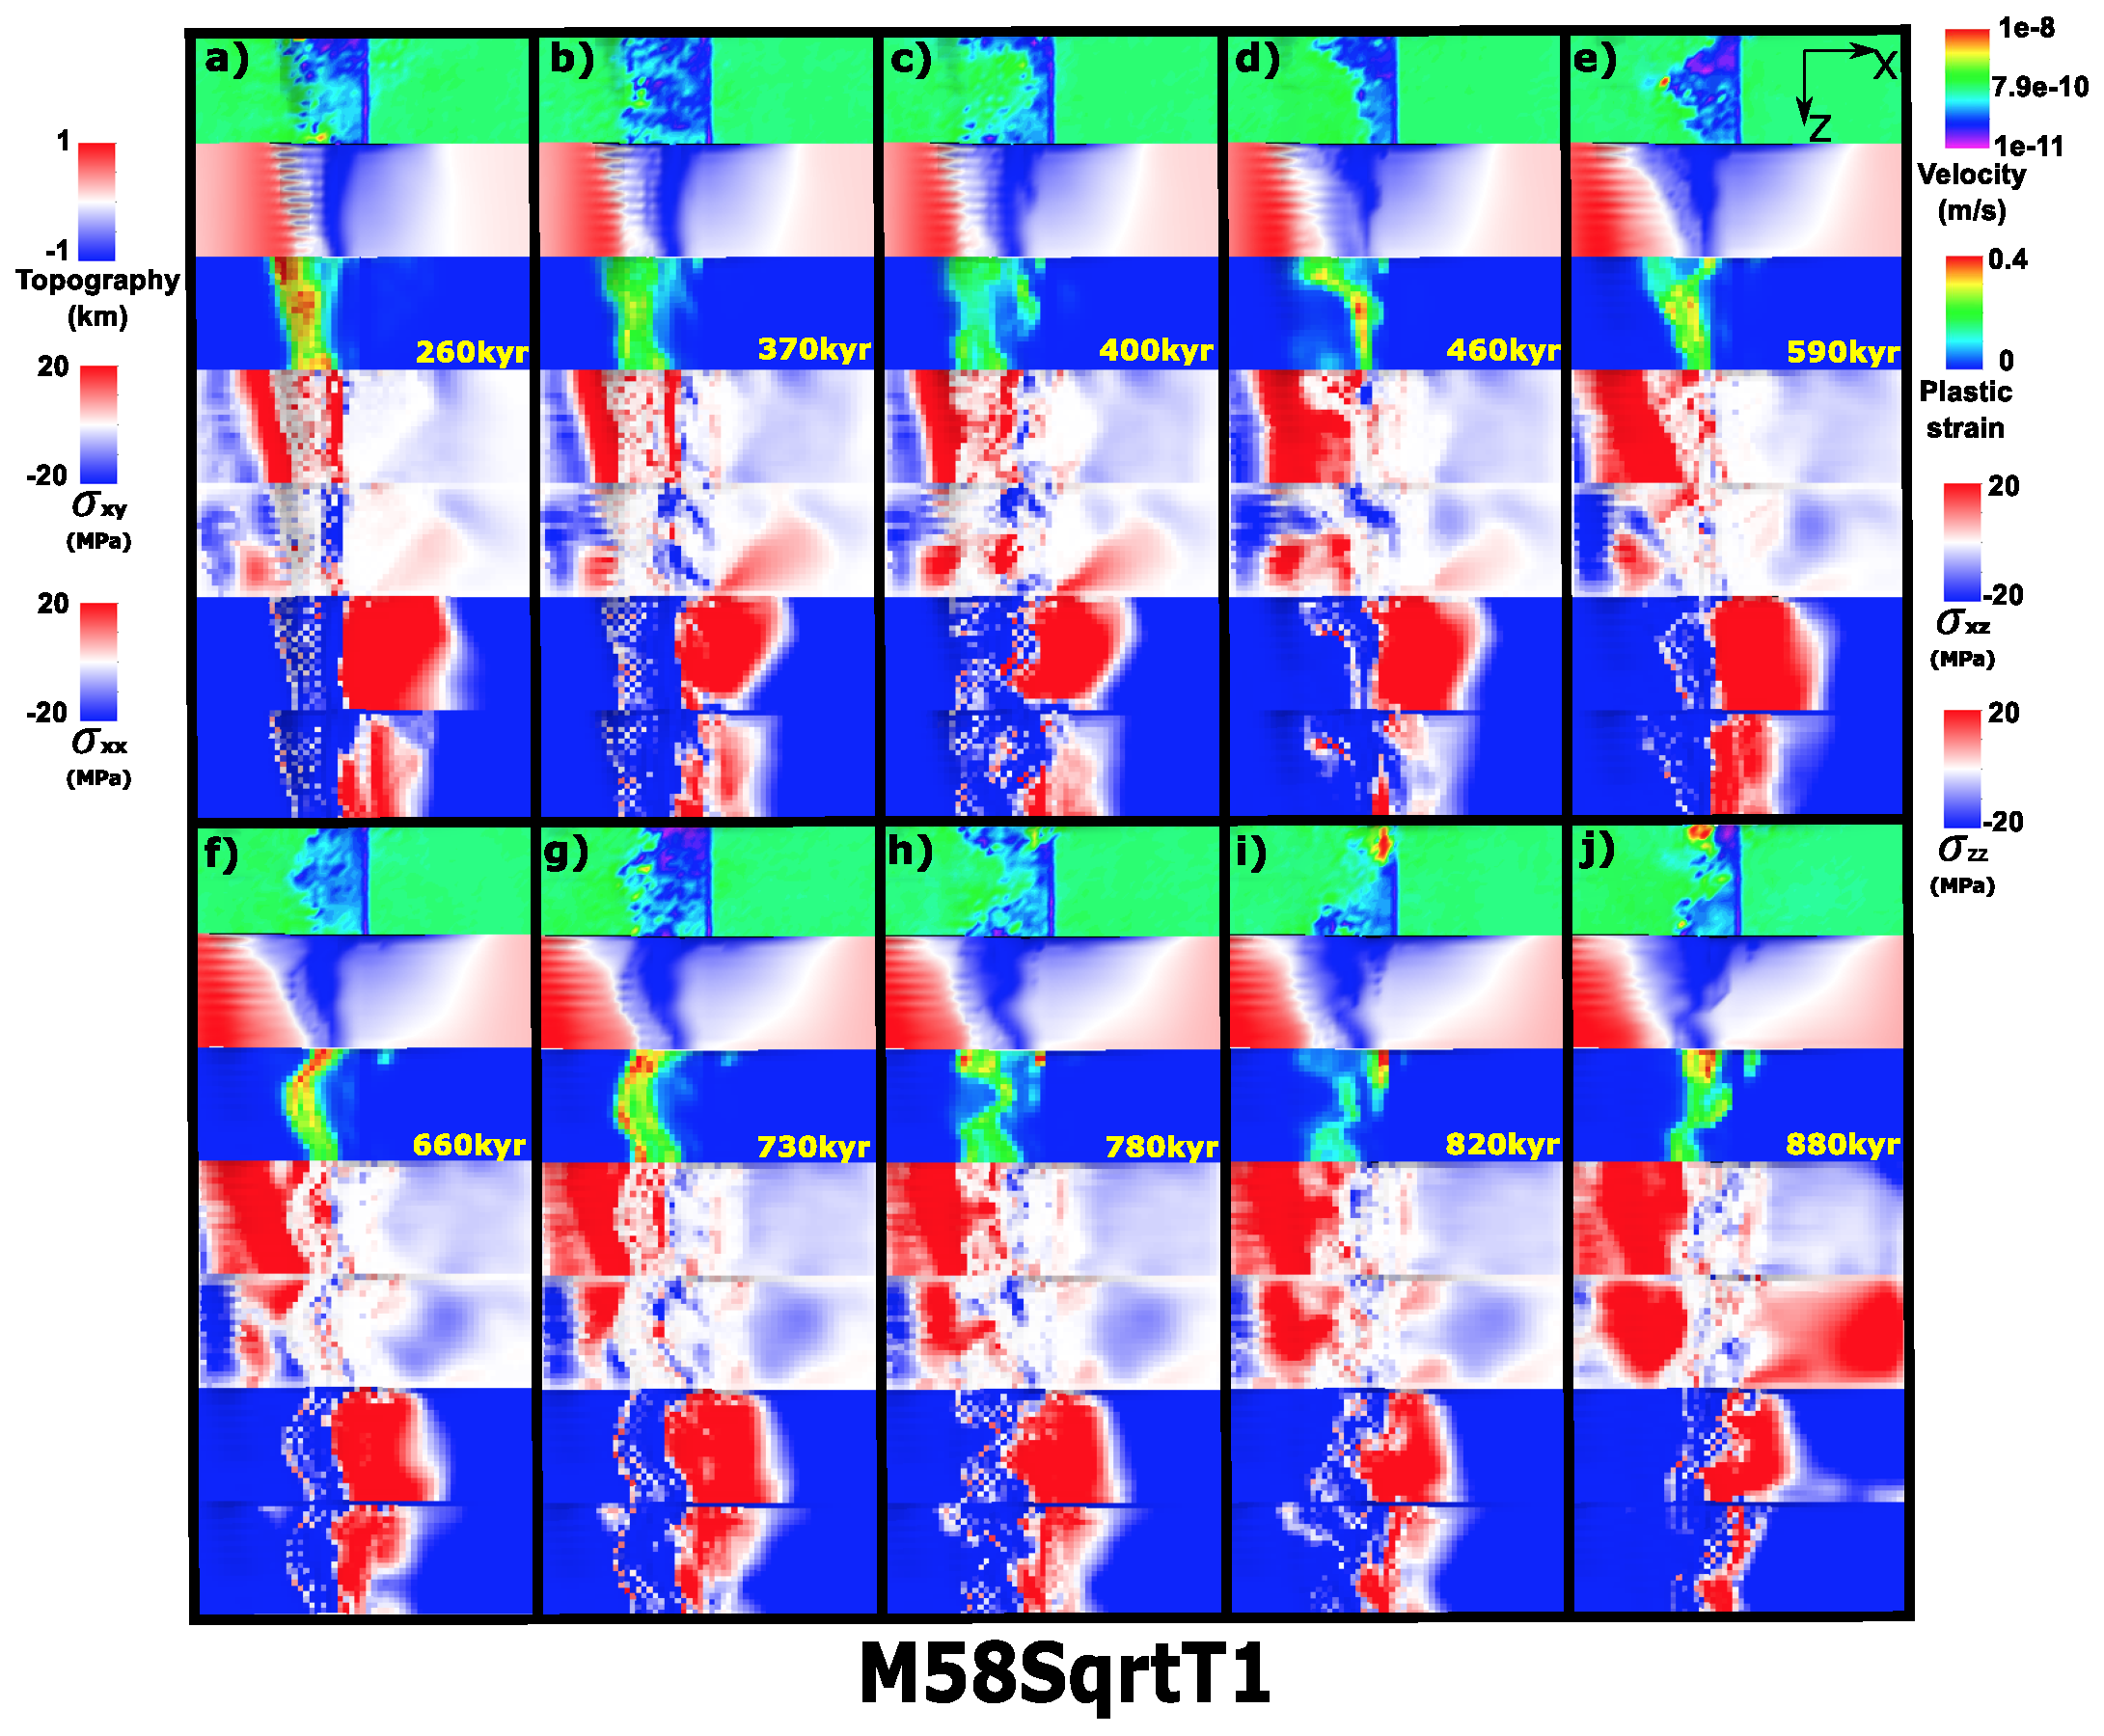
\includegraphics[width=1.0\textwidth]{./Figures/fig_Results_Weakening_7_M58SqrtT1_time_evolution.eps}
 \caption{Bird's-eye view of faulting and stresses evolution of M58SqrtT1.}
\label{fig_Results_Weakenging_7}
\end{figure}

\begin{figure}[h]
\noindent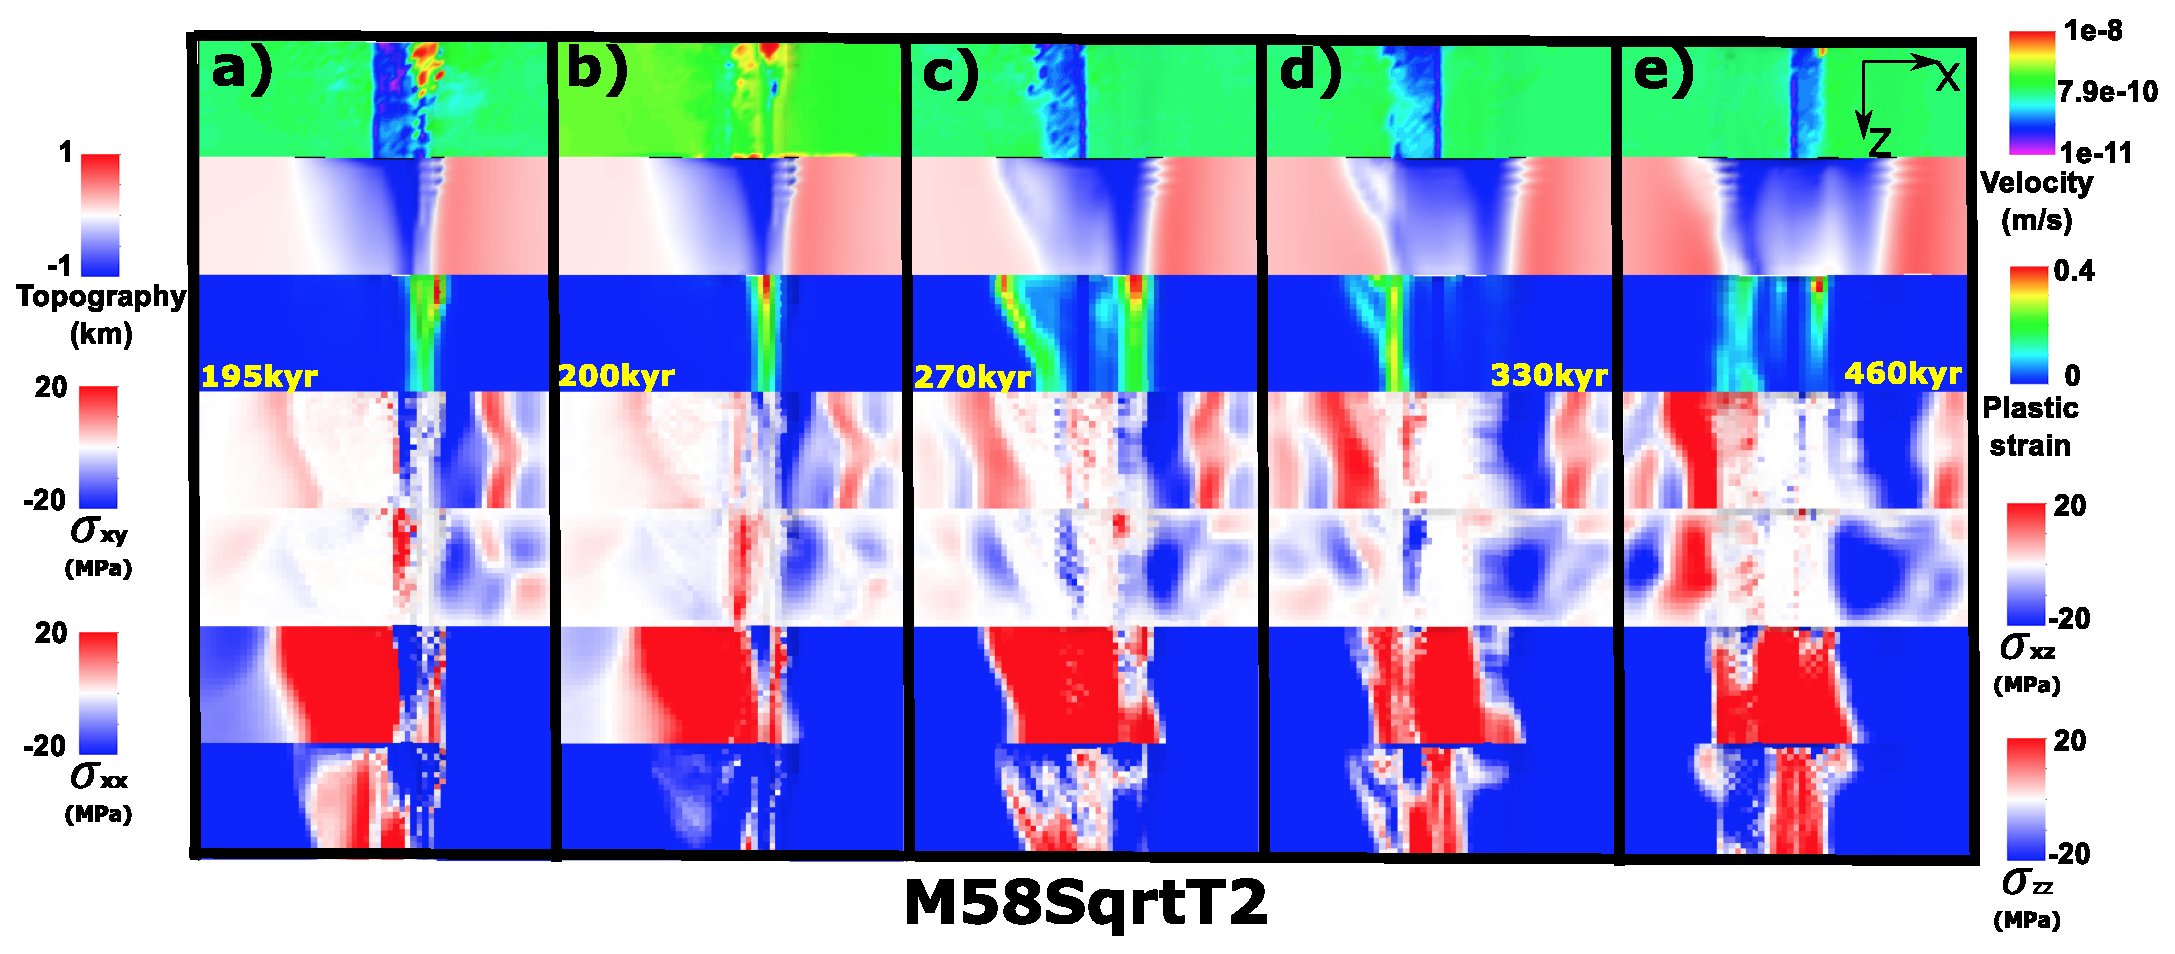
\includegraphics[width=1.0\textwidth]{./Figures/fig_Results_Weakening_8_M58SqrtT2_time_evolution.eps}
 \caption{Faulting and stresses evolution for M58SqrtT2.}
\label{fig_Results_Weakenging_8}
\end{figure}

\begin{figure}[h]
\noindent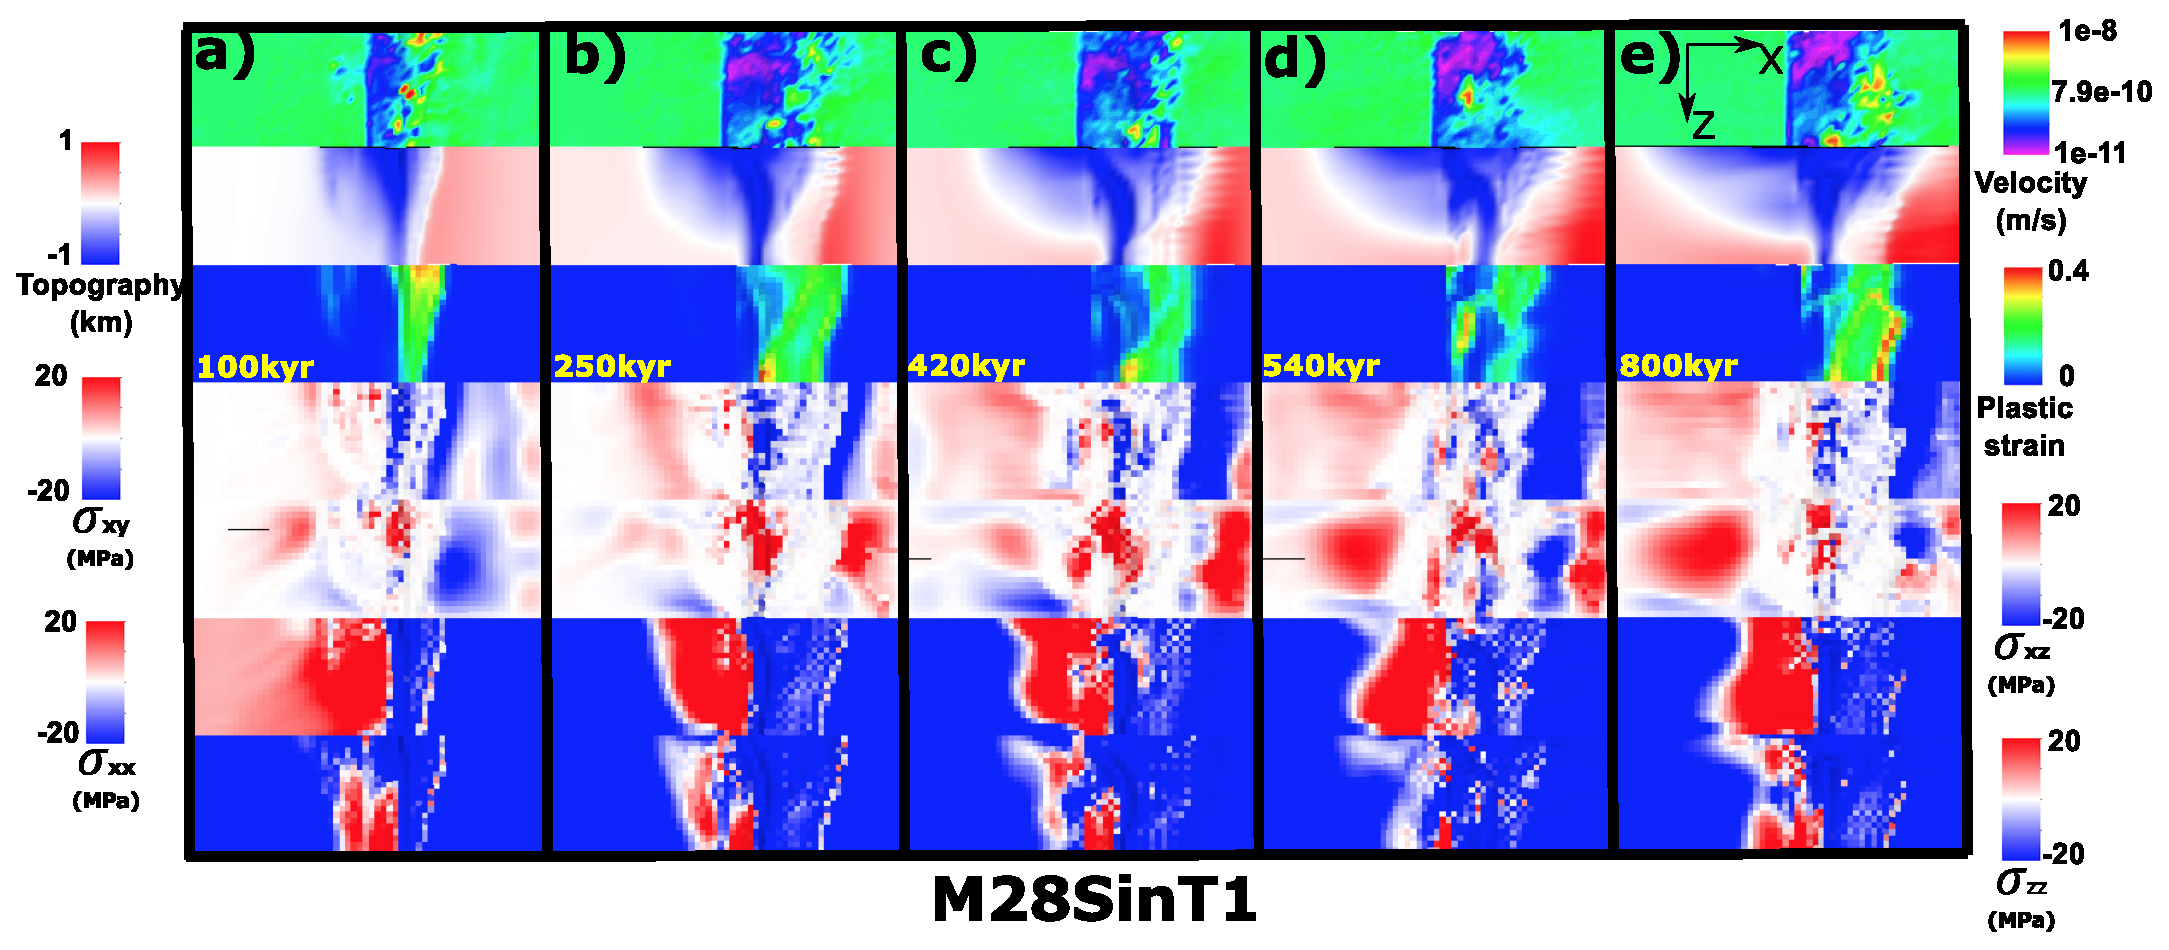
\includegraphics[width=1.0\textwidth]{./Figures/fig_Results_MRange_1_M28SinT1_time_evolution.eps}
 \caption{M28SinT1 (Table~\ref{Tab1_1}) faulting and stresses evolution with respect to time.}
\label{fig_Results_MRange_1}
\end{figure}

\begin{figure}[h]
\noindent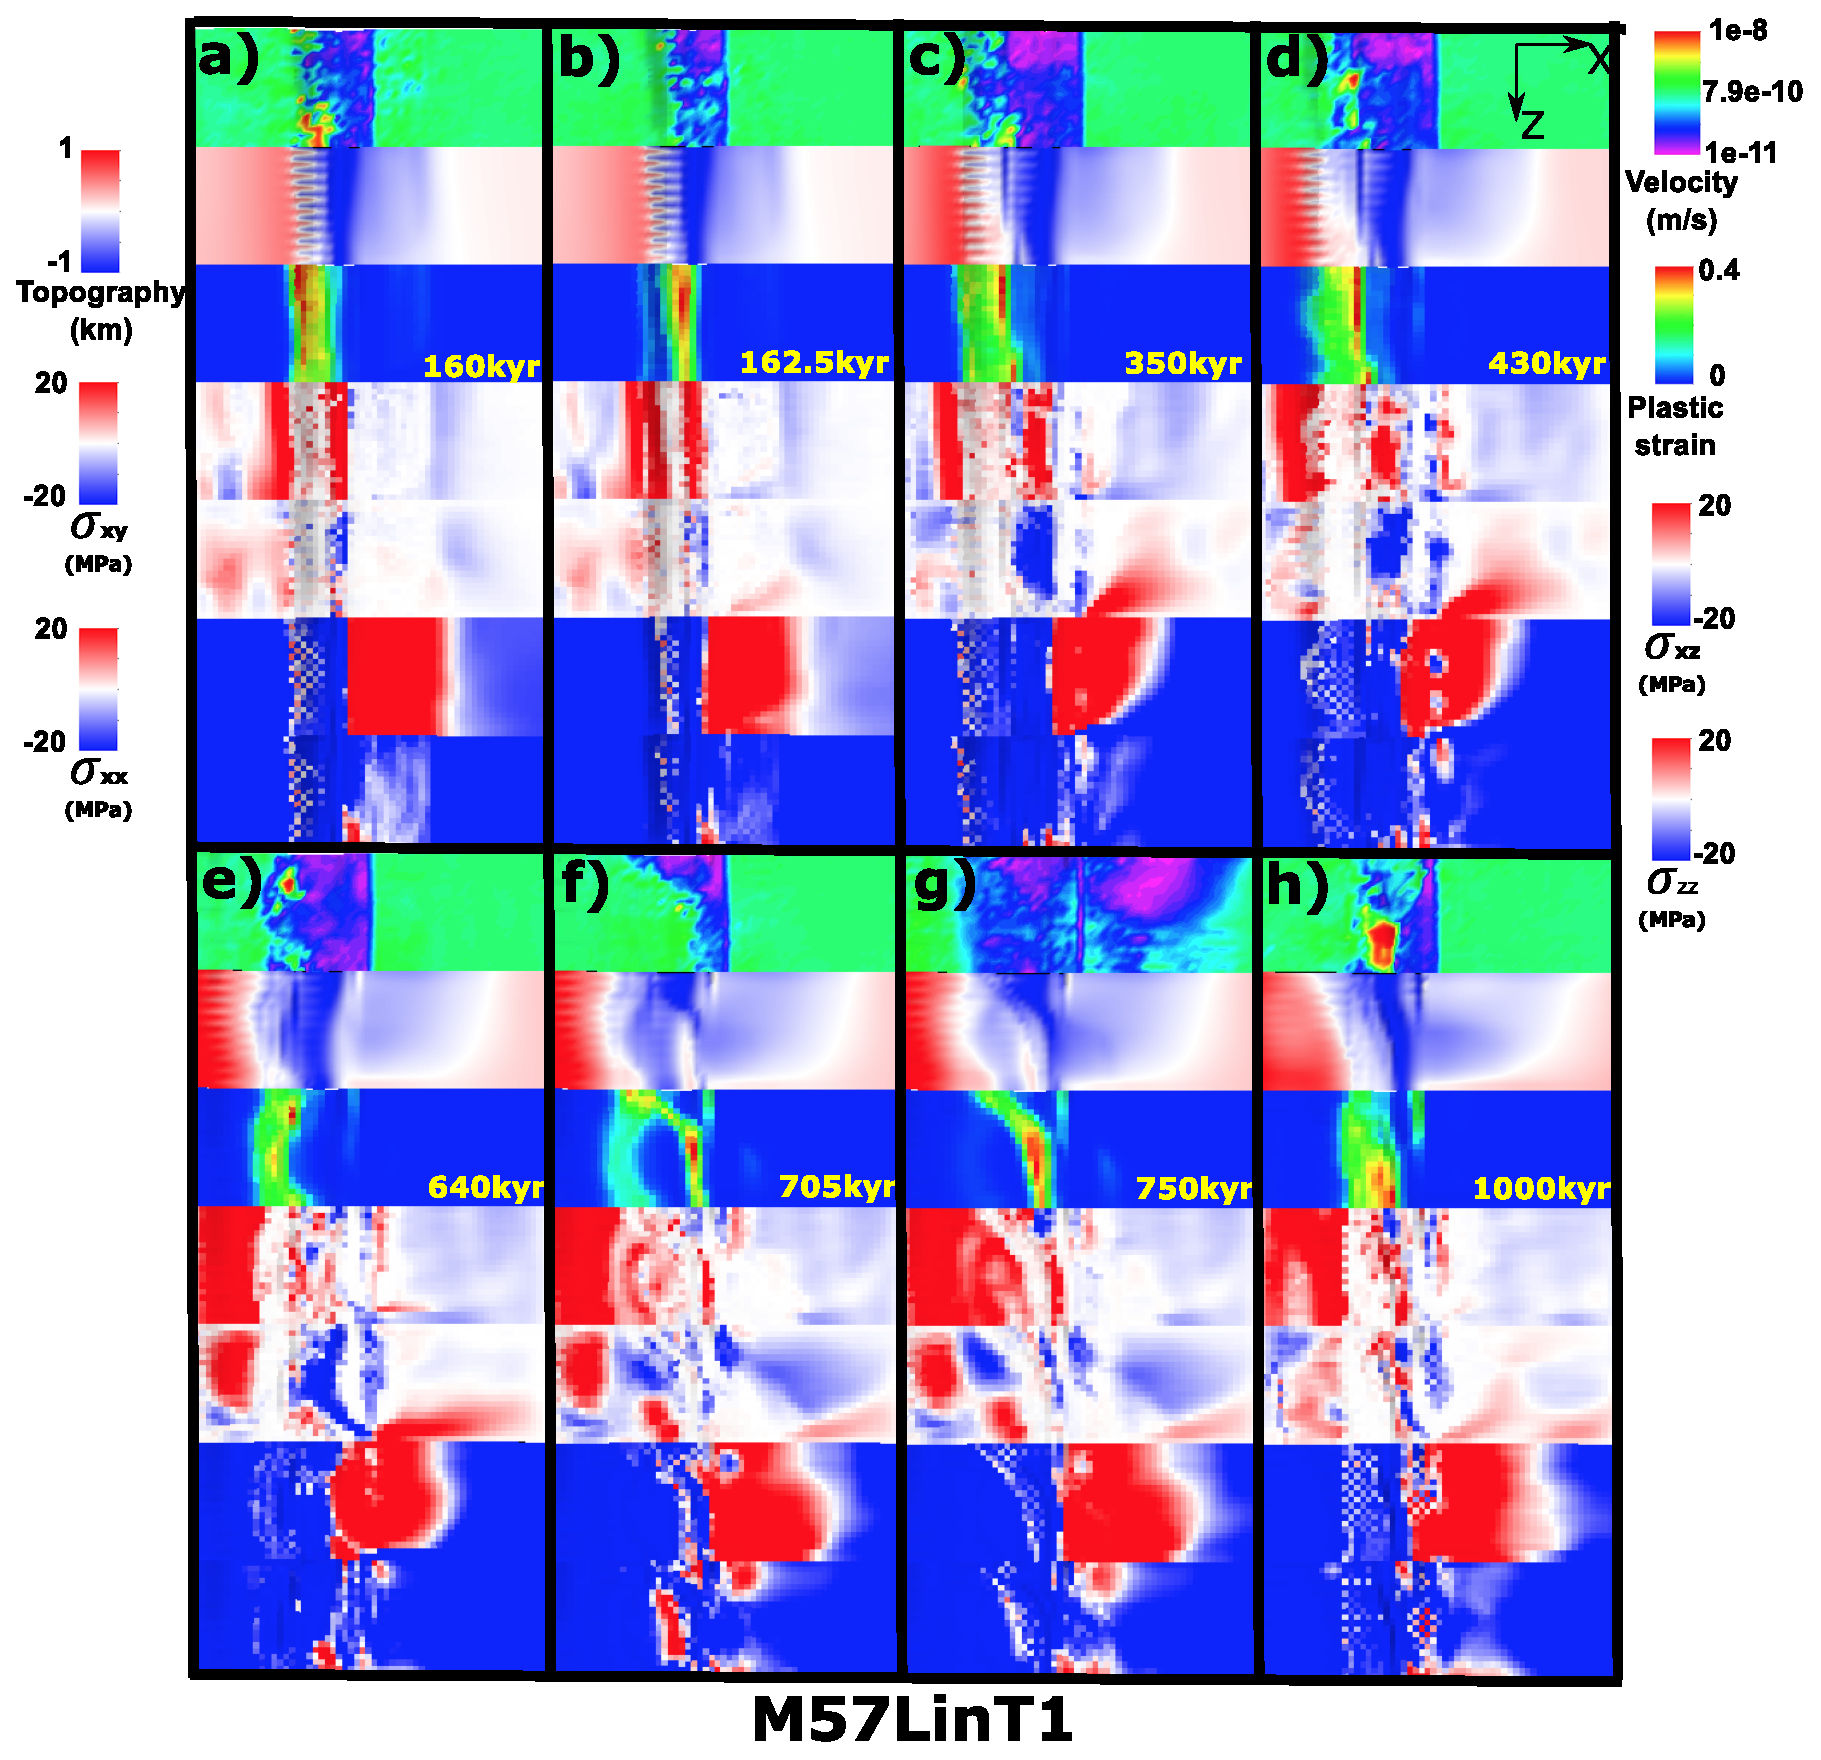
\includegraphics[width=0.8\textwidth]{./Figures/fig_Results_MRange_2_M57LinT1_time_evolution.eps}
 \caption{M57LinT1 (Table~\ref{Tab1_1}) faulting and stresses evolution with respect to time.}
\label{fig_Results_MRange_2}
\end{figure}

\begin{figure}[h]
\noindent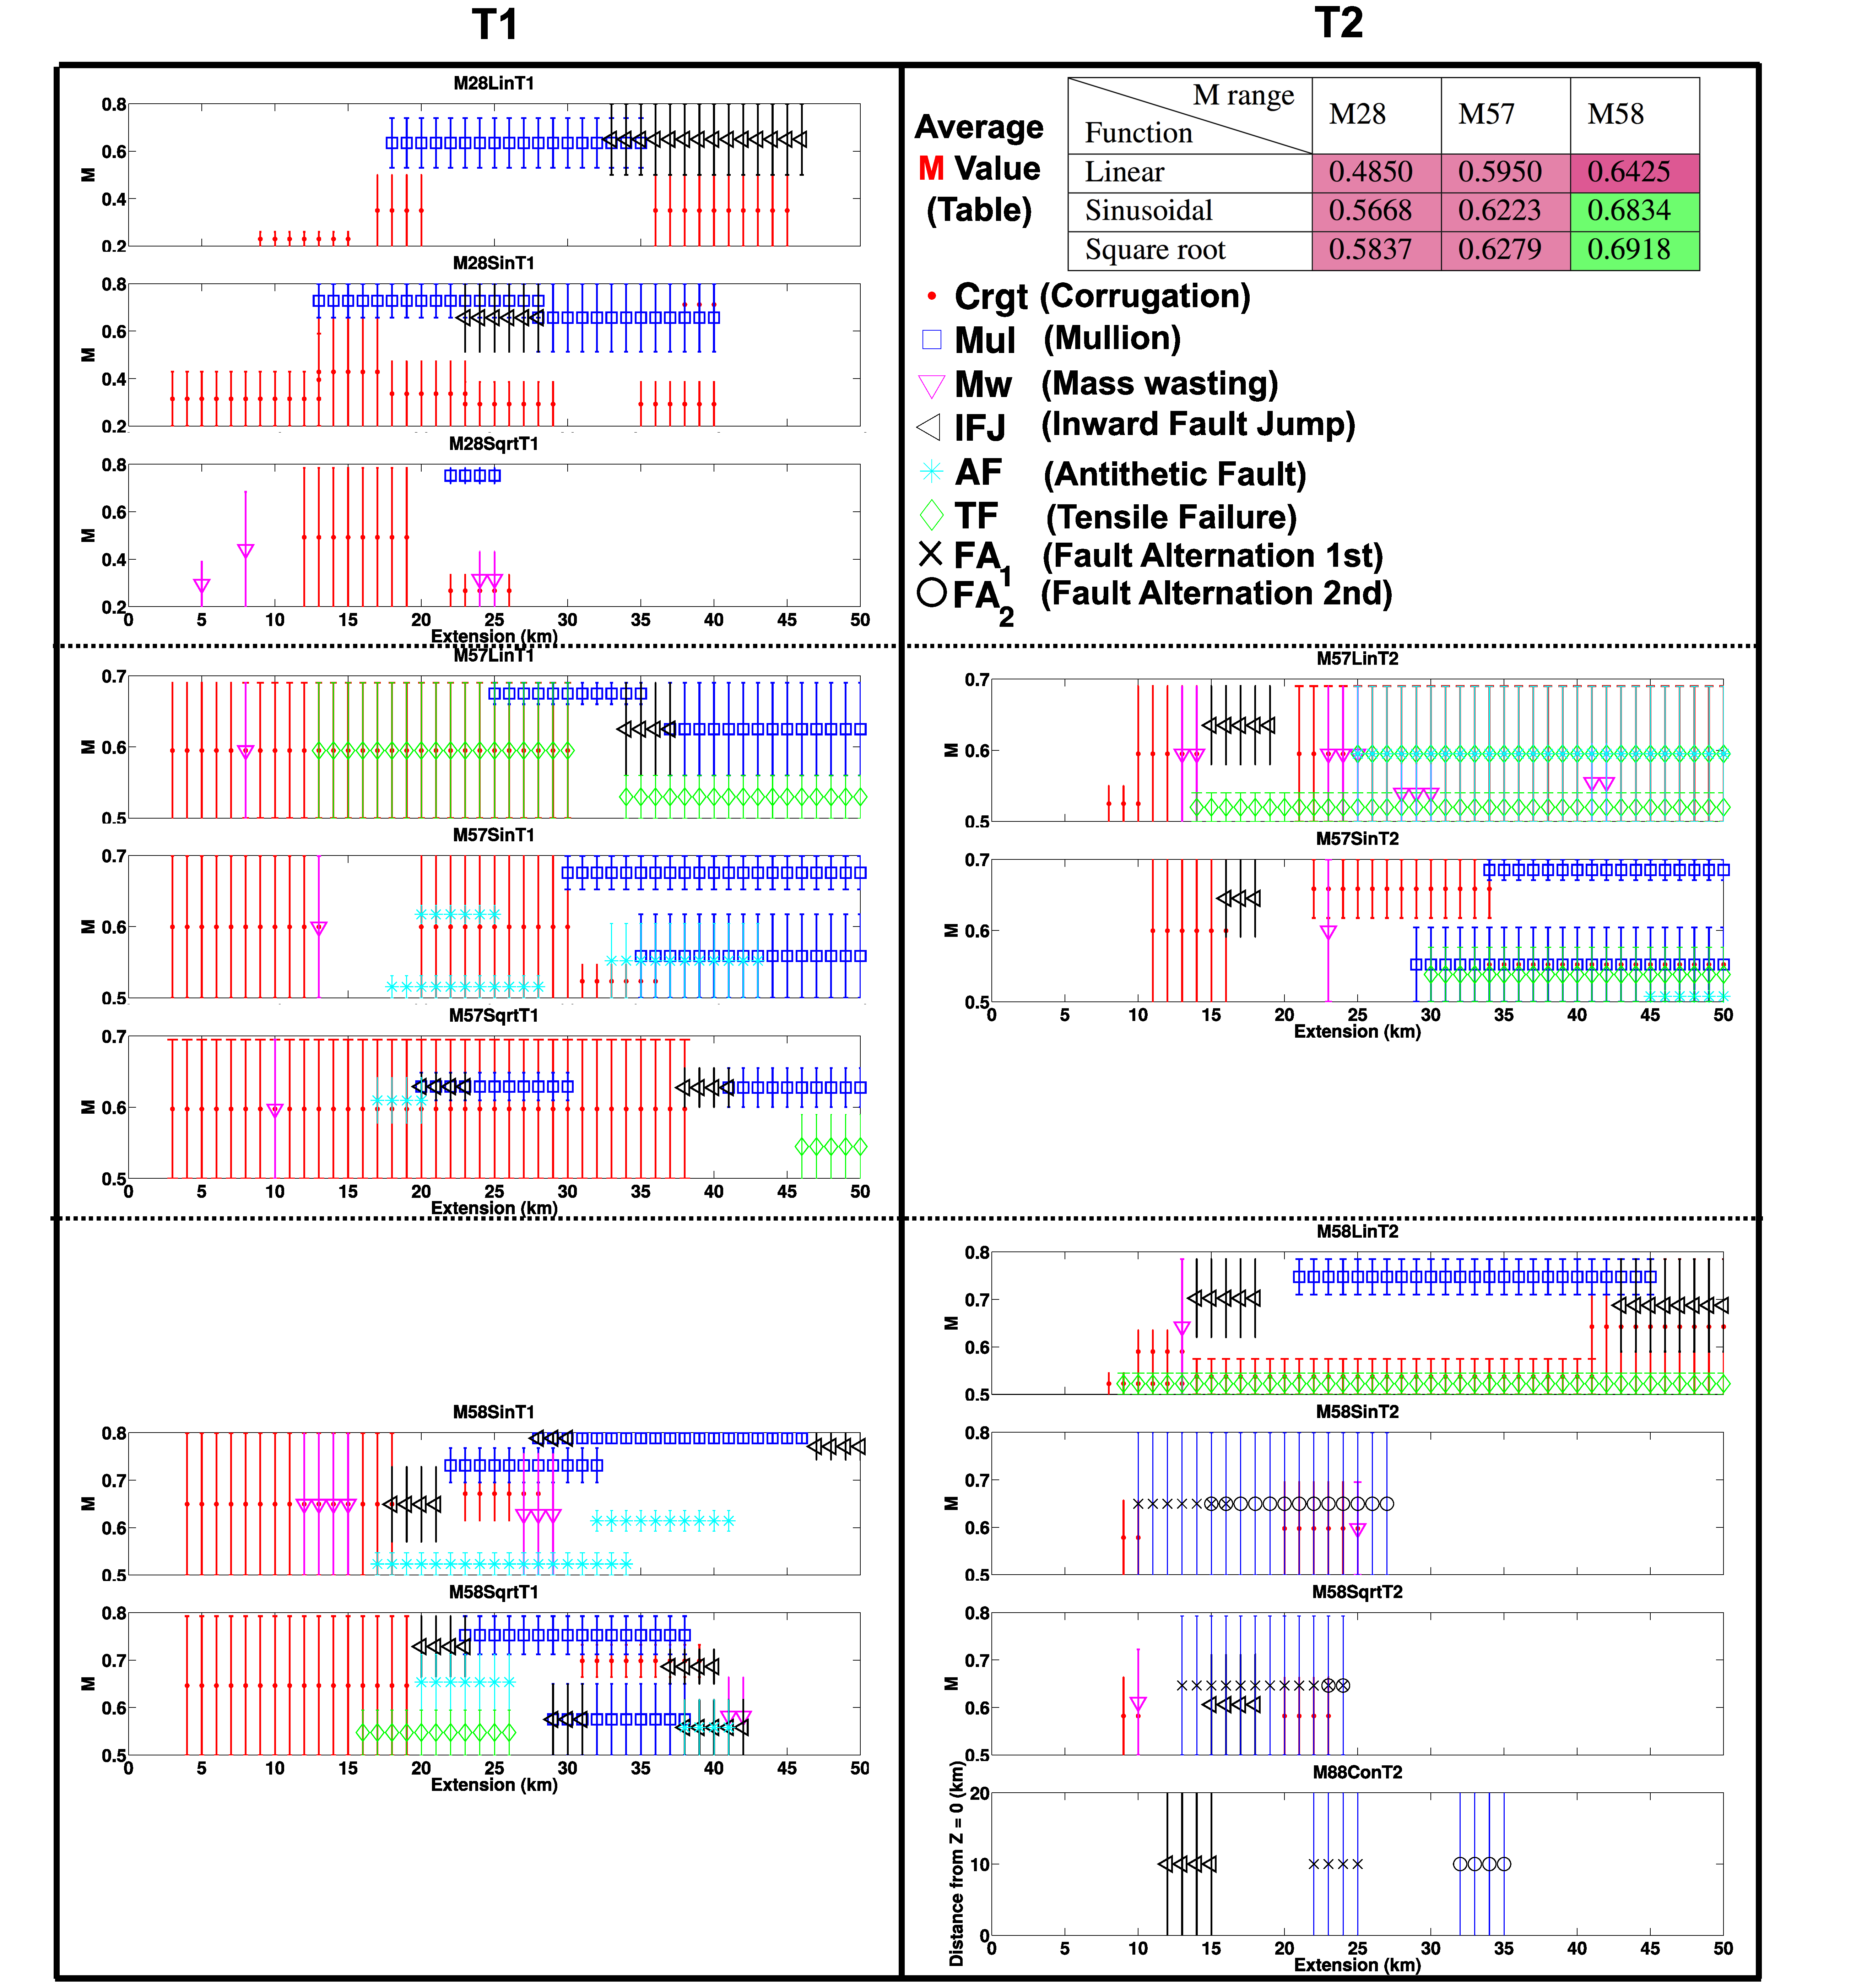
\includegraphics[width=0.926\textwidth]{./Figures/fig_Discussion_Result_Summary_1_Combine_together.eps}
    \caption{Initiation and duration of main structural features.}
 \label{fig_Discussion_Result_Summary_1_Combine_together}
\end{figure} 

\begin{figure}[h]
\noindent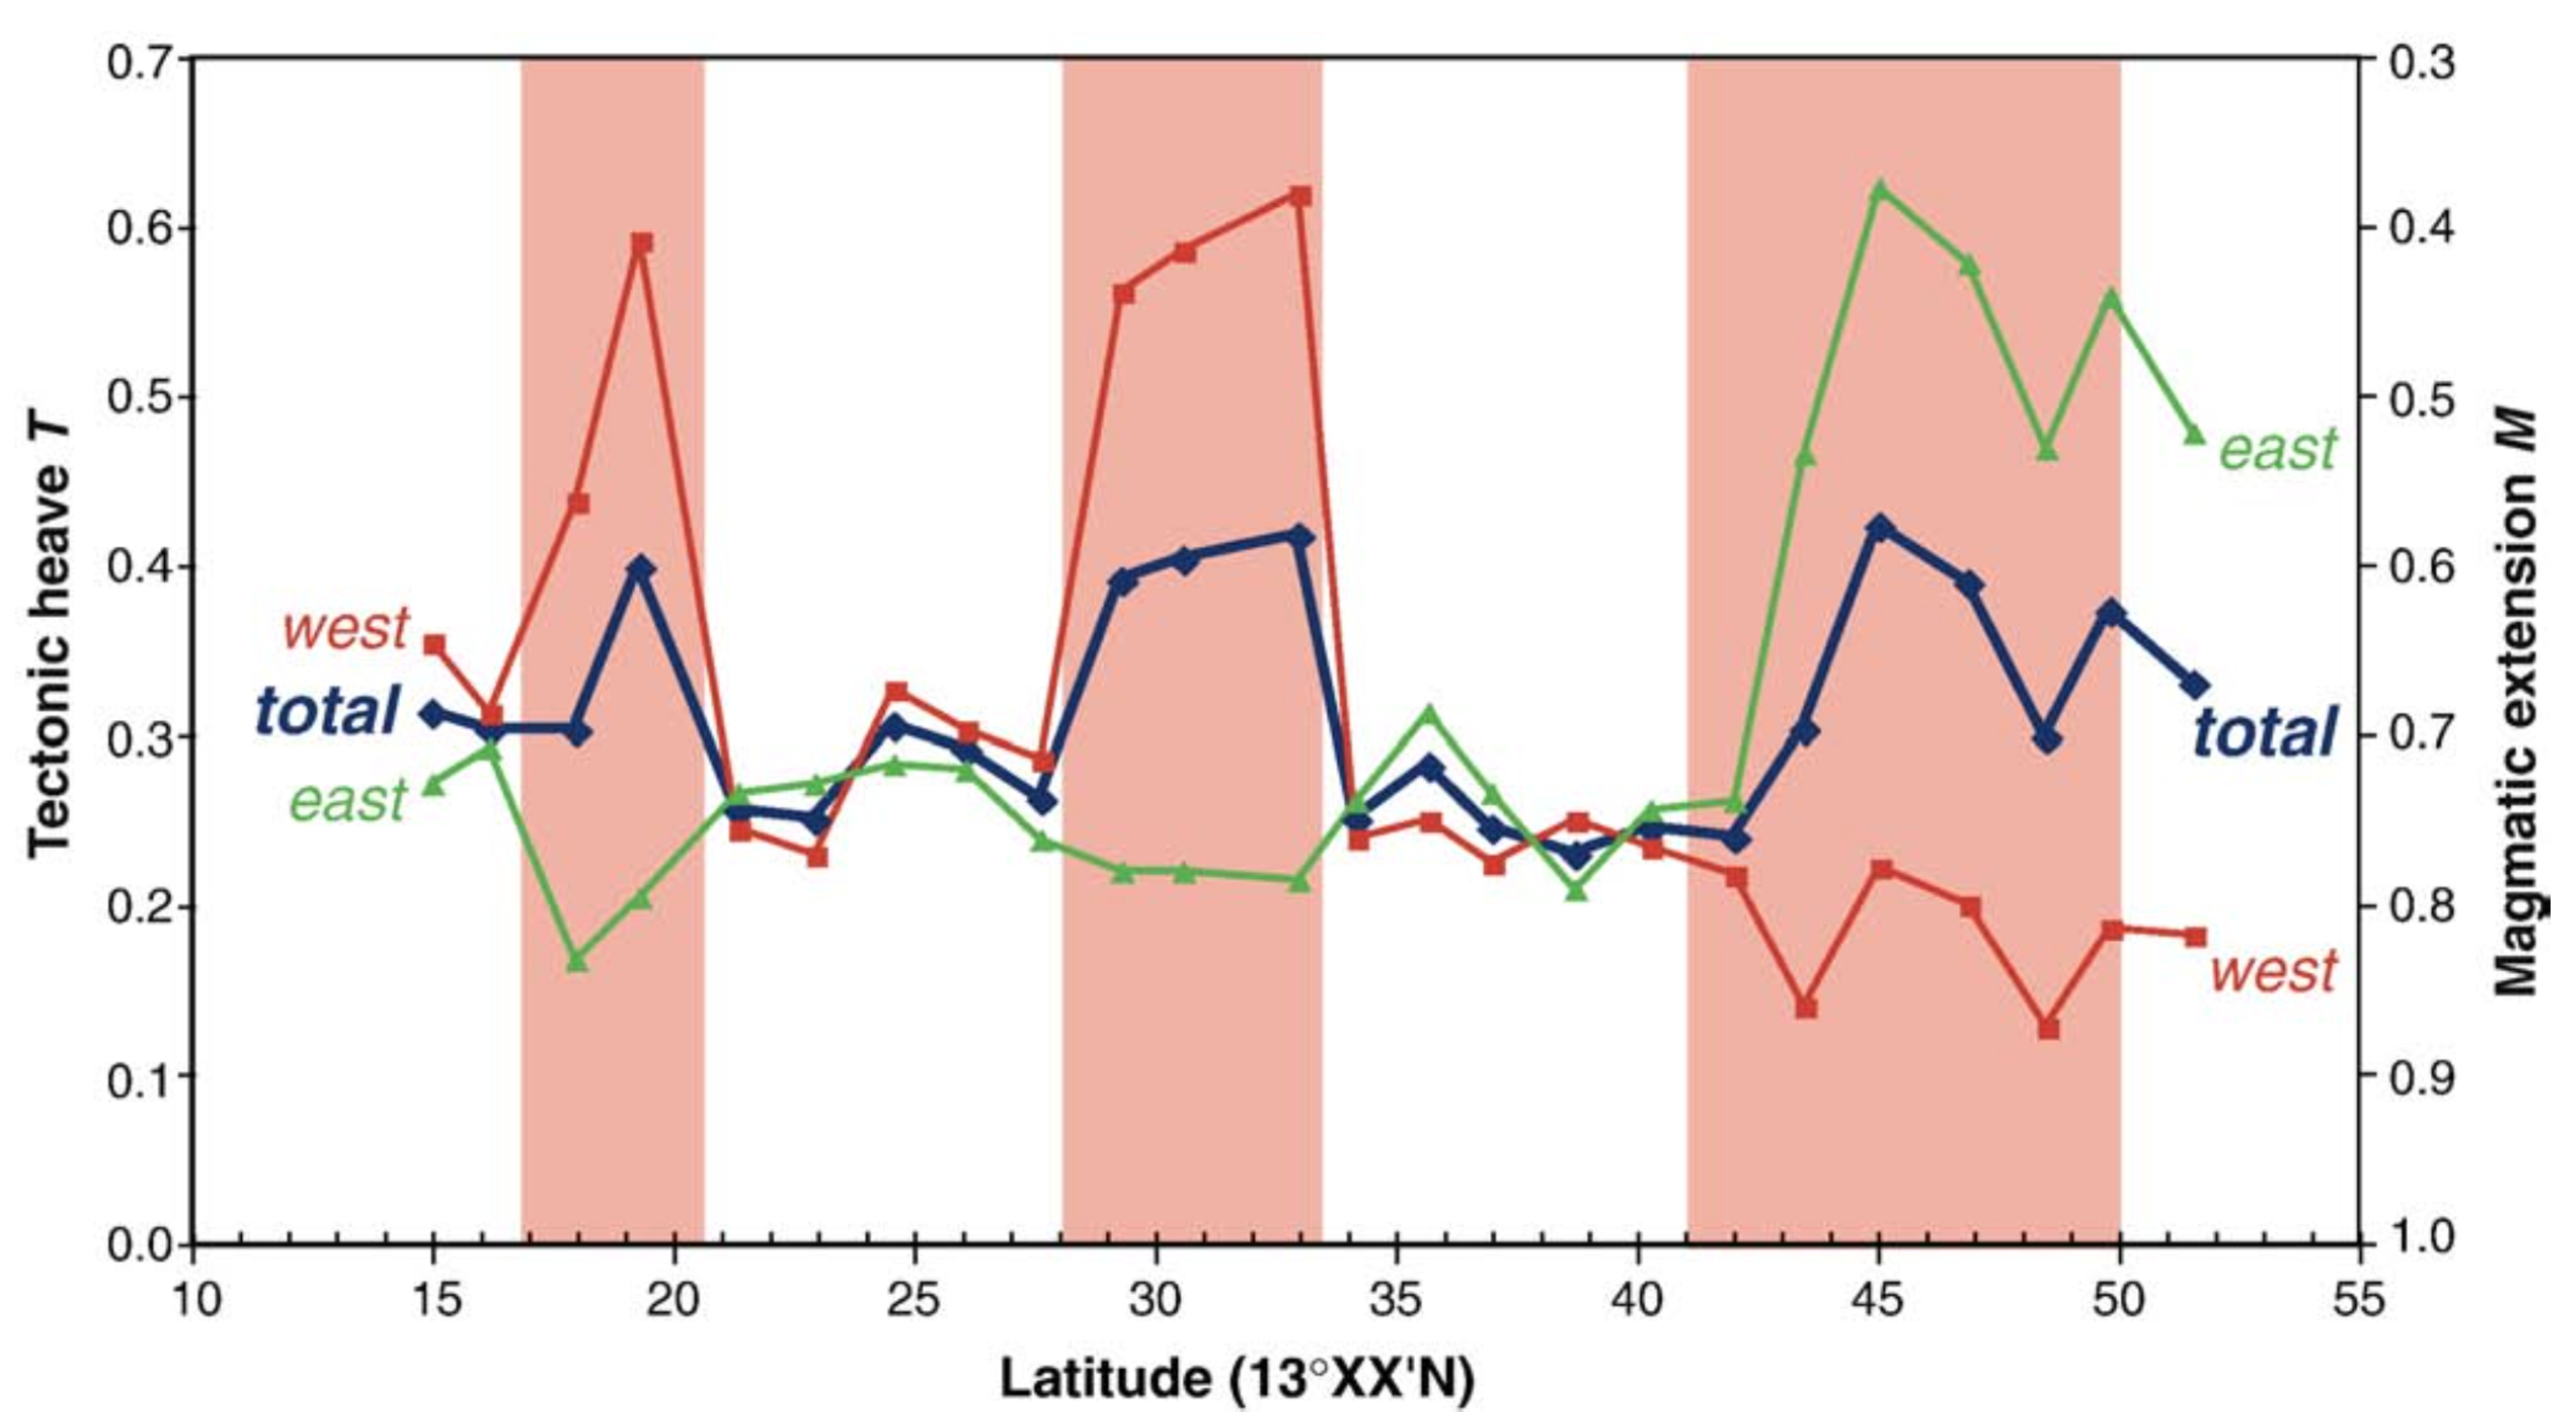
\includegraphics[width=1\textwidth]{./Figures/fig_Discussion_ResultsSummary_MacLeod2009.eps}
 \caption[Field observation results adapted from \citep{MacLeod2009}.]{Along-axis variations in total accumulated tectonic heave T in the past 1.86 Ma (since chron C2n), and consequent inferred magmatic component M (= 1 $-$ T) as a proportion of total plate separation (blue line). Pink shaded areas delineate loci of the active or recently active OCCs. The relative contributions of tectonic strain from the western and eastern flanks of the axis that give rise to the total heave T are shown by red and green lines respectively. Adapted from \citep{MacLeod2009}. }
 \label{fig_Discussion_ResultsSummary_MacLeod2009}
\end{figure}

\begin{figure}[h]
\noindent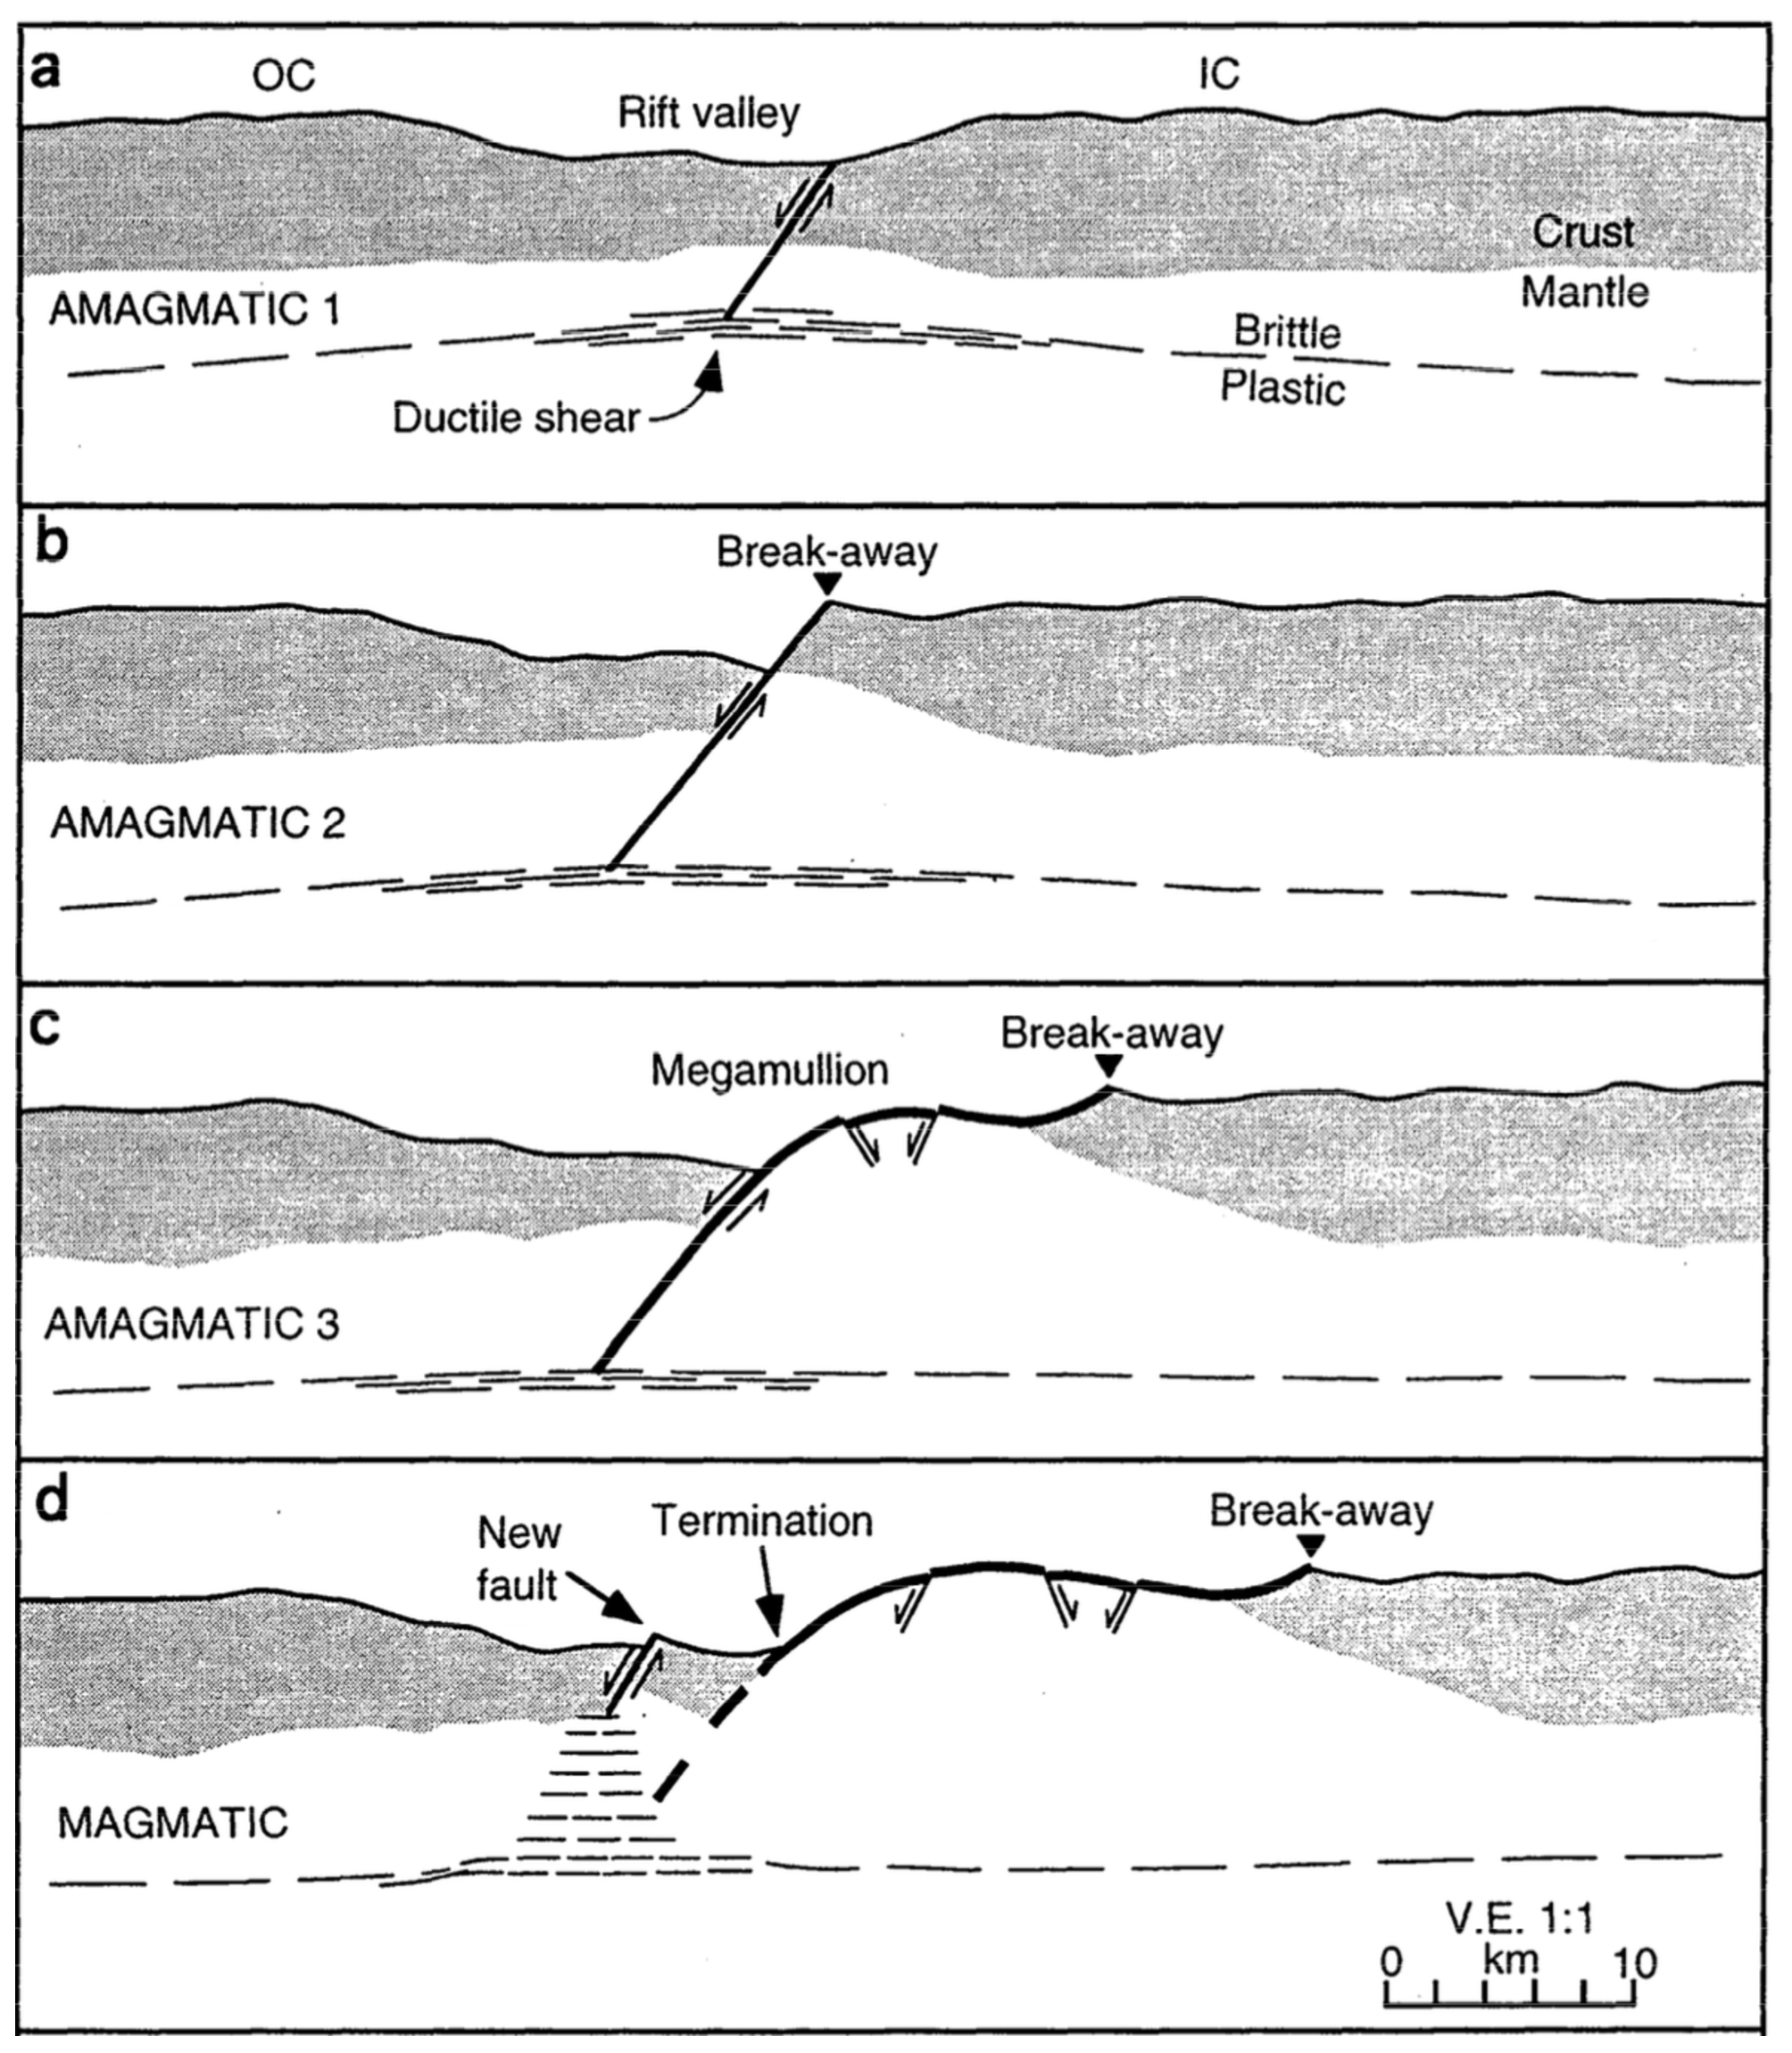
\includegraphics[width=0.7\textwidth]{./Figures/fig_Discussion_Observation_1_Tucholke1998.eps}
 \caption[Schematic development of a megamullion from amagmatic to magmatic, adapted from \citep{Tucholke1998}.]{Schematic development of a megamullion. No vertical exaggeration. (a)$\sim$(c) shows the detachment fault evolution during amagmatic phase. (d) Increased magma supply pushed the detachment fault away from ridge axis and forms a new normal fault near the ridge axis (``inward fault jump''). Adapted from \citep{Tucholke1998}.}
 \label{fig_Discussion_Observation_1_Tucholke1998}
\end{figure}

\begin{figure}[h]
\noindent\includegraphics[width=1.0\textwidth]{./Figures/fig_Discussion_Observation_2_Dick2008_Kane.eps}
 \caption[Bathymetric map and simplified tectonic interpretation of Kane Megamullion. Adapted from \citep{Dick2008}.]{Bathymetric map and simplified tectonic interpretation of Kane Megamullion. Contour interval is 100 m. Pie diagrams show lithologic proportions by weight in dredge and dive collections. Detachemtn fault breakaway and termination are marked as dashed lines. Shaded regions indicate areas of possible off-axis volcanism. Adapted from \citep{Dick2008}.}
 \label{fig_Discussion_Observation_2_Dick2008_Kane}
\end{figure}

\begin{figure}[h]
\noindent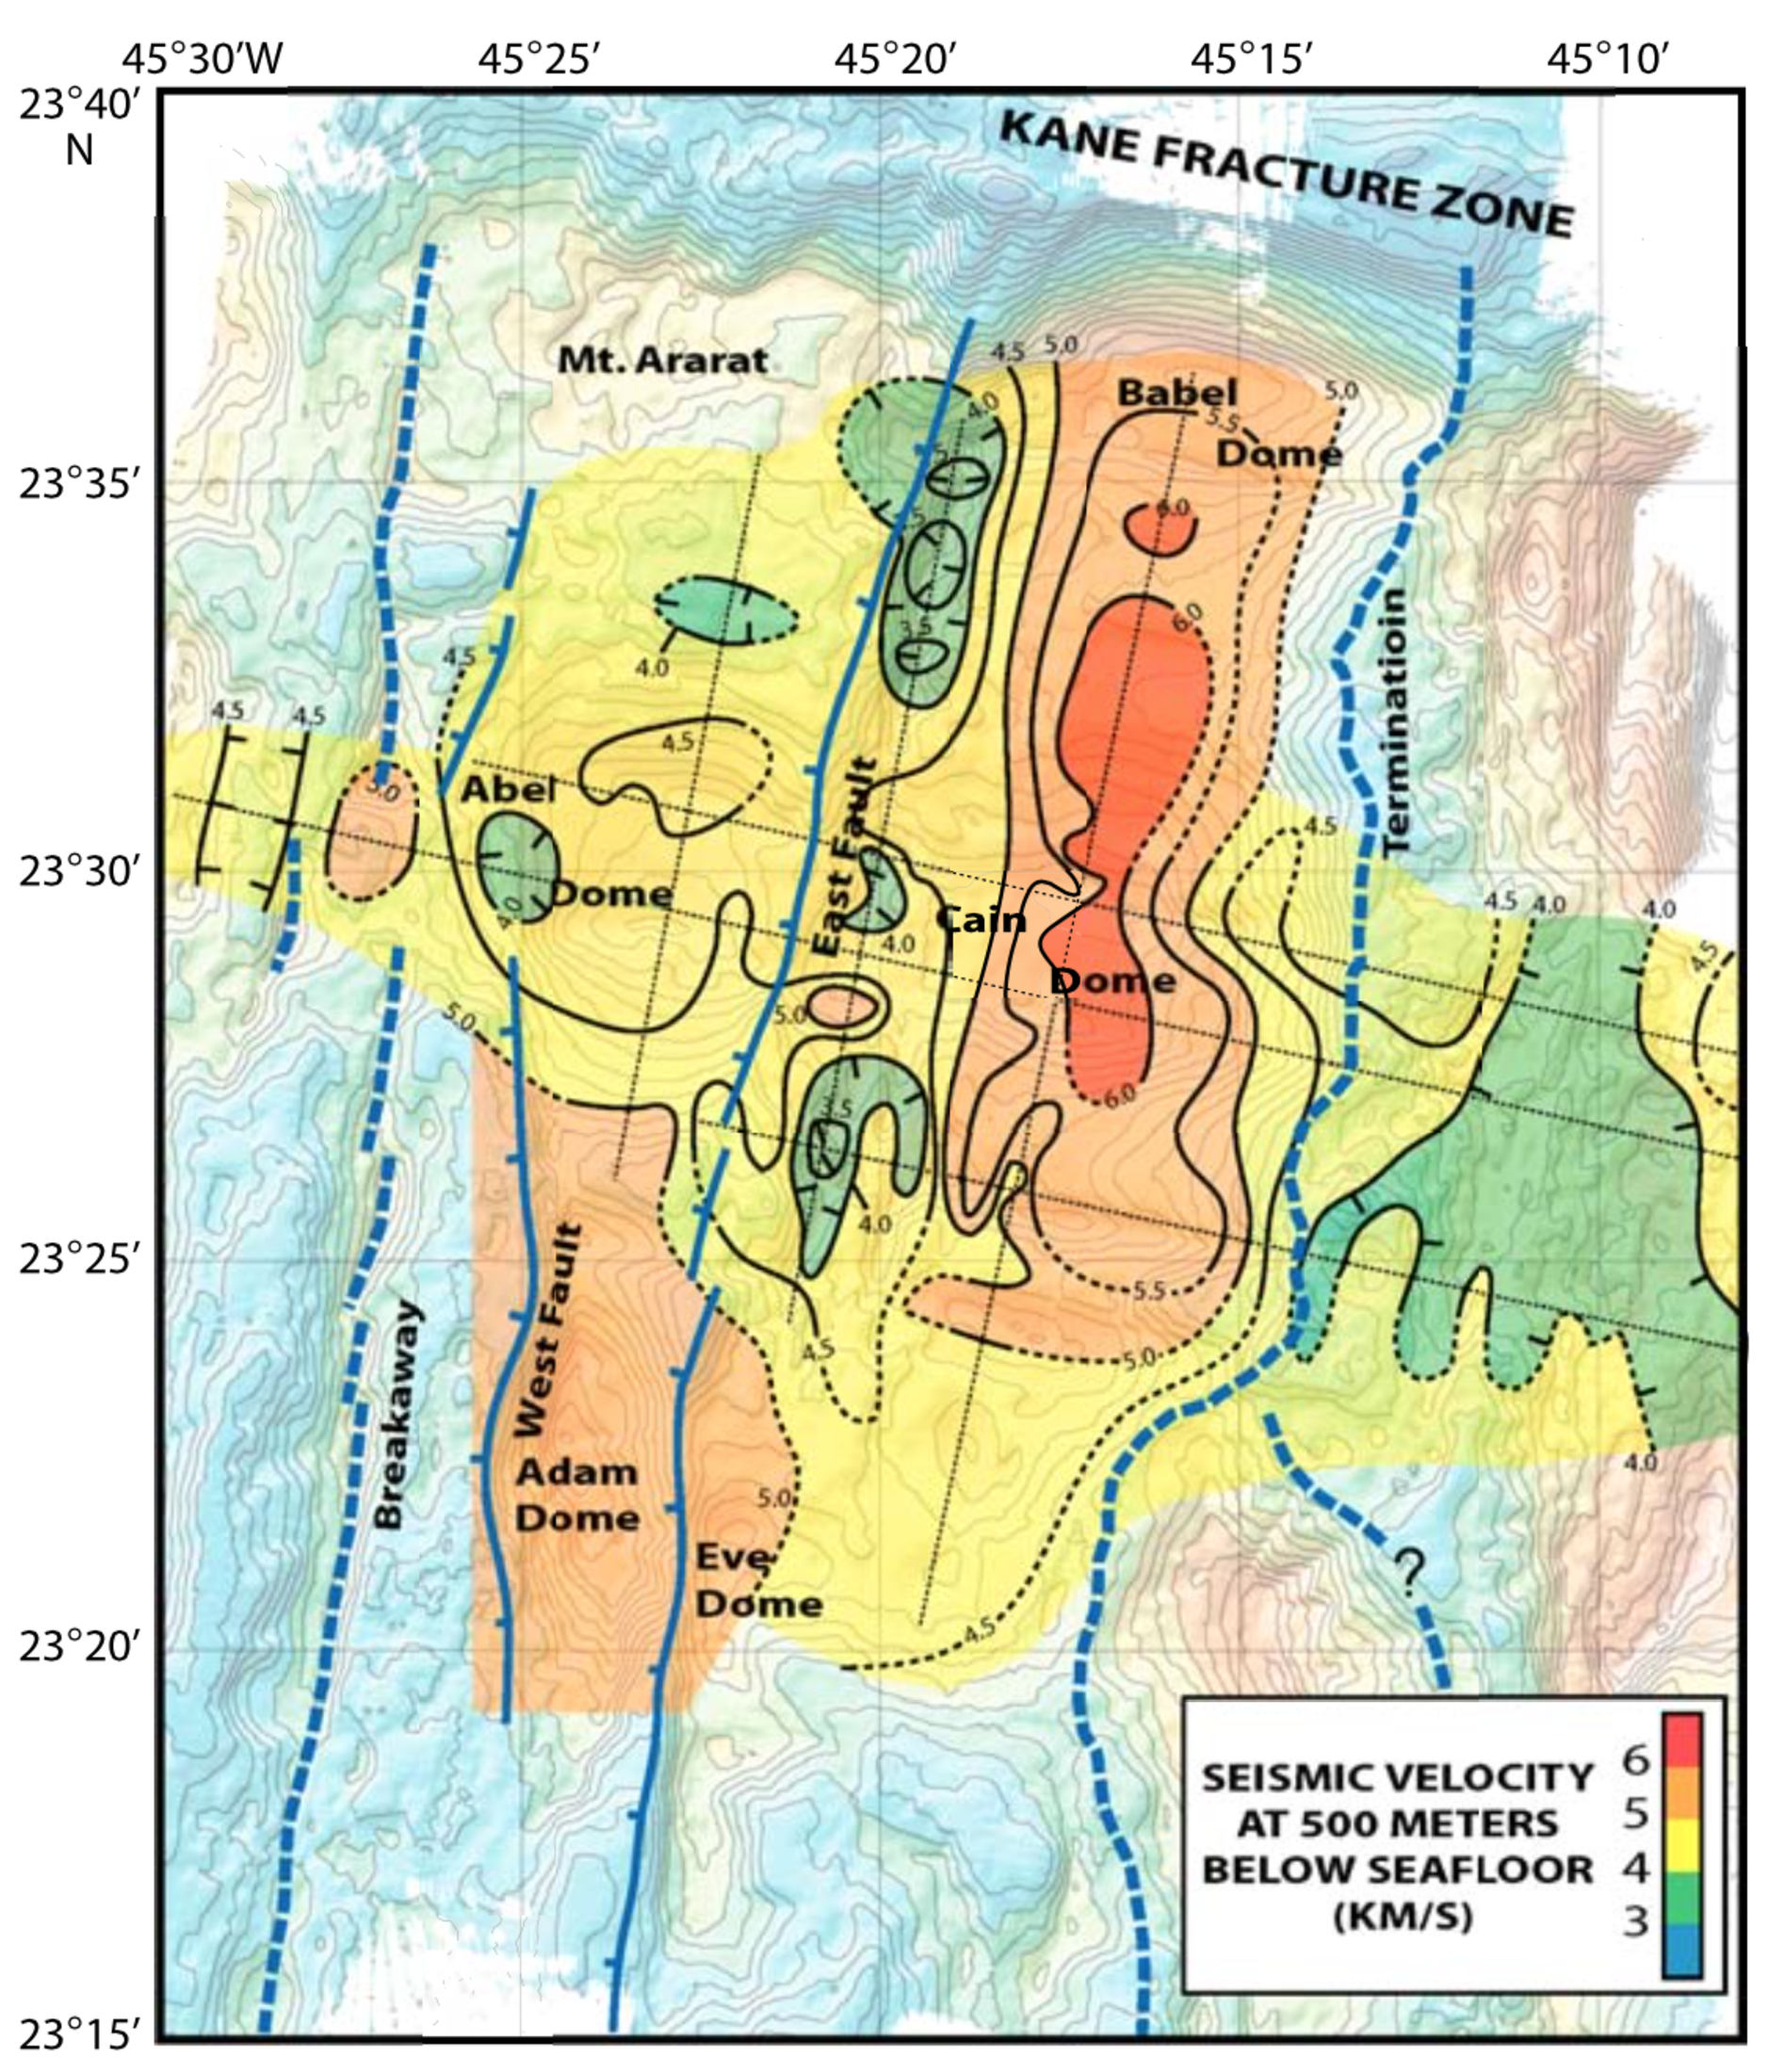
\includegraphics[width=0.6\textwidth]{./Figures/fig_Discussion_Observation_1_Xu2009_SeismicV_Kane.eps}
 \caption{P wave isovelocity contours at 500 m below seafloor superimposed on bathymetry and simplified tectonic interpretation. Adapted from \citep{Xu2009}.}
 \label{fig_Discussion_Observation_1_Xu2009_SeismicV_Kane}
\end{figure}

\begin{figure}[h]
\noindent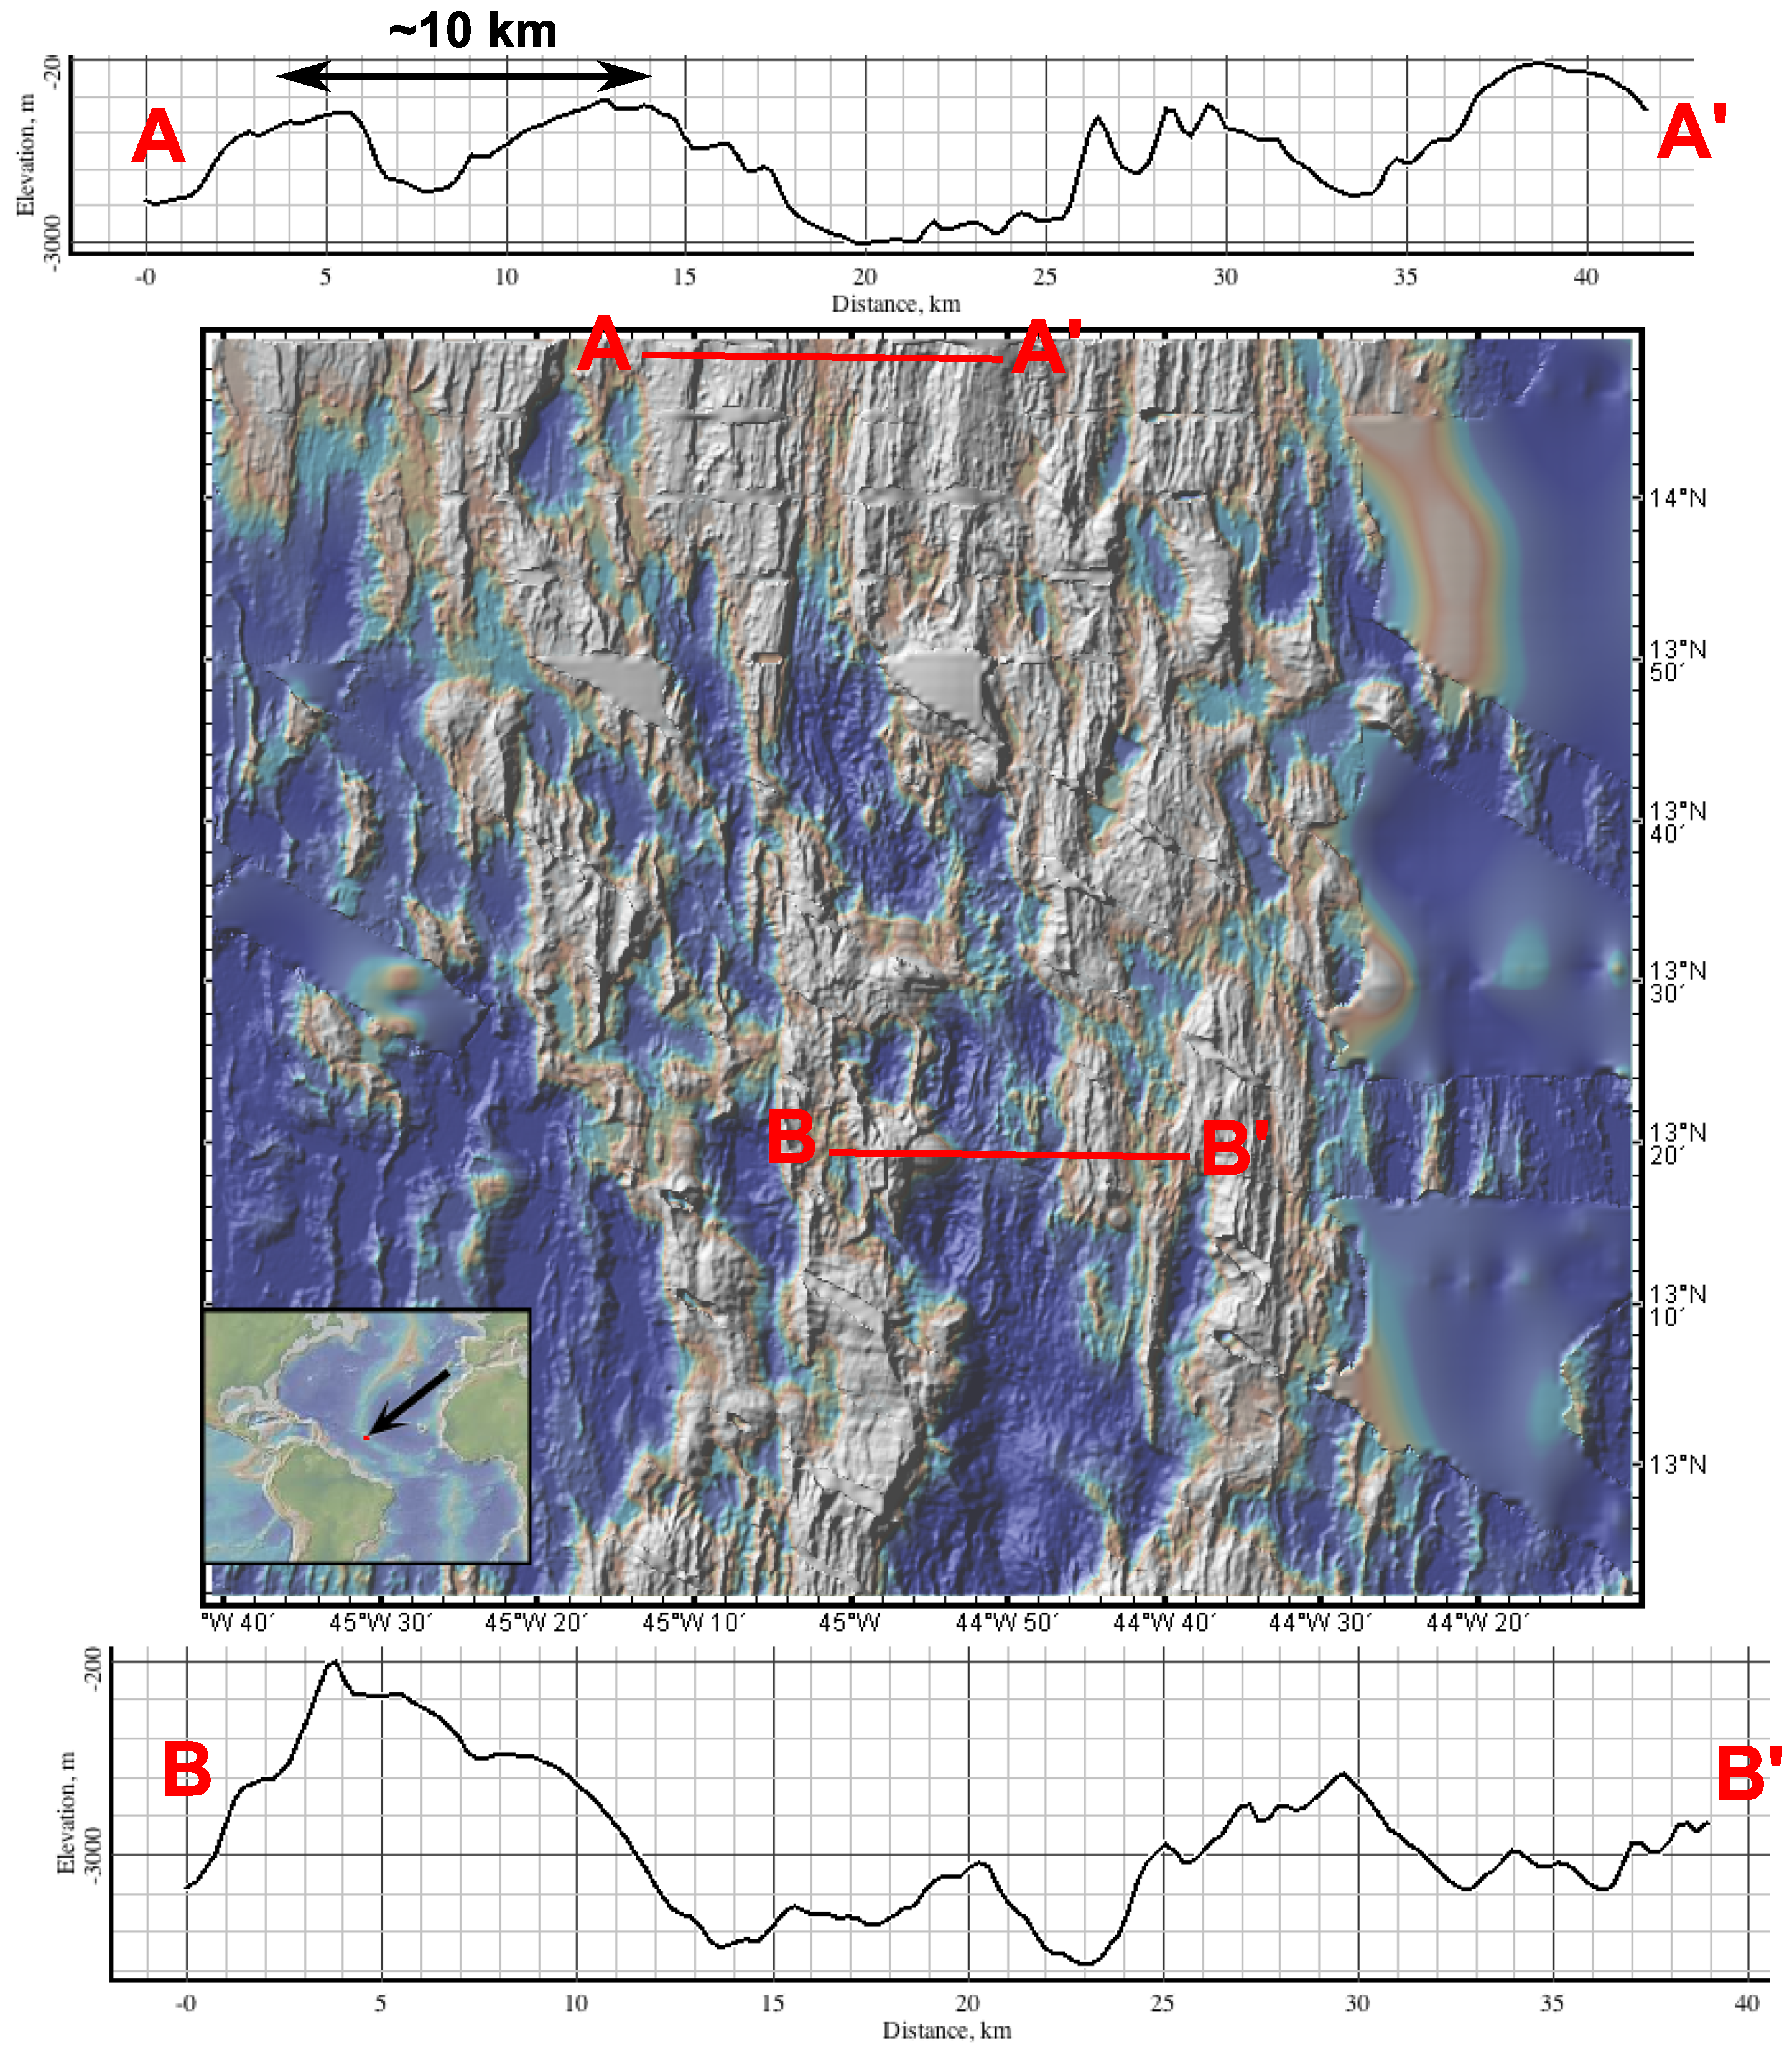
\includegraphics[width=0.75\textwidth]{./Figures/fig_Discussion_Observation_2_13-14N_MAR.eps}
 \caption[Bathymetry from 12.8$\sim$14.2 $\degree$N Mid-Atlantic Ridge.]{Bathymetry from 12.8$\sim$14.2 $\degree$N Mid-Atlantic Ridge. Crossection A$\sim$A$^{\prime}$ and B$\sim$B$^{\prime}$ are 5 times vertical exagerated. From GeoMapApp.}
 \label{fig_Discussion_Observation_2_13-14N_MAR}
\end{figure}

\begin{figure}[h]
\noindent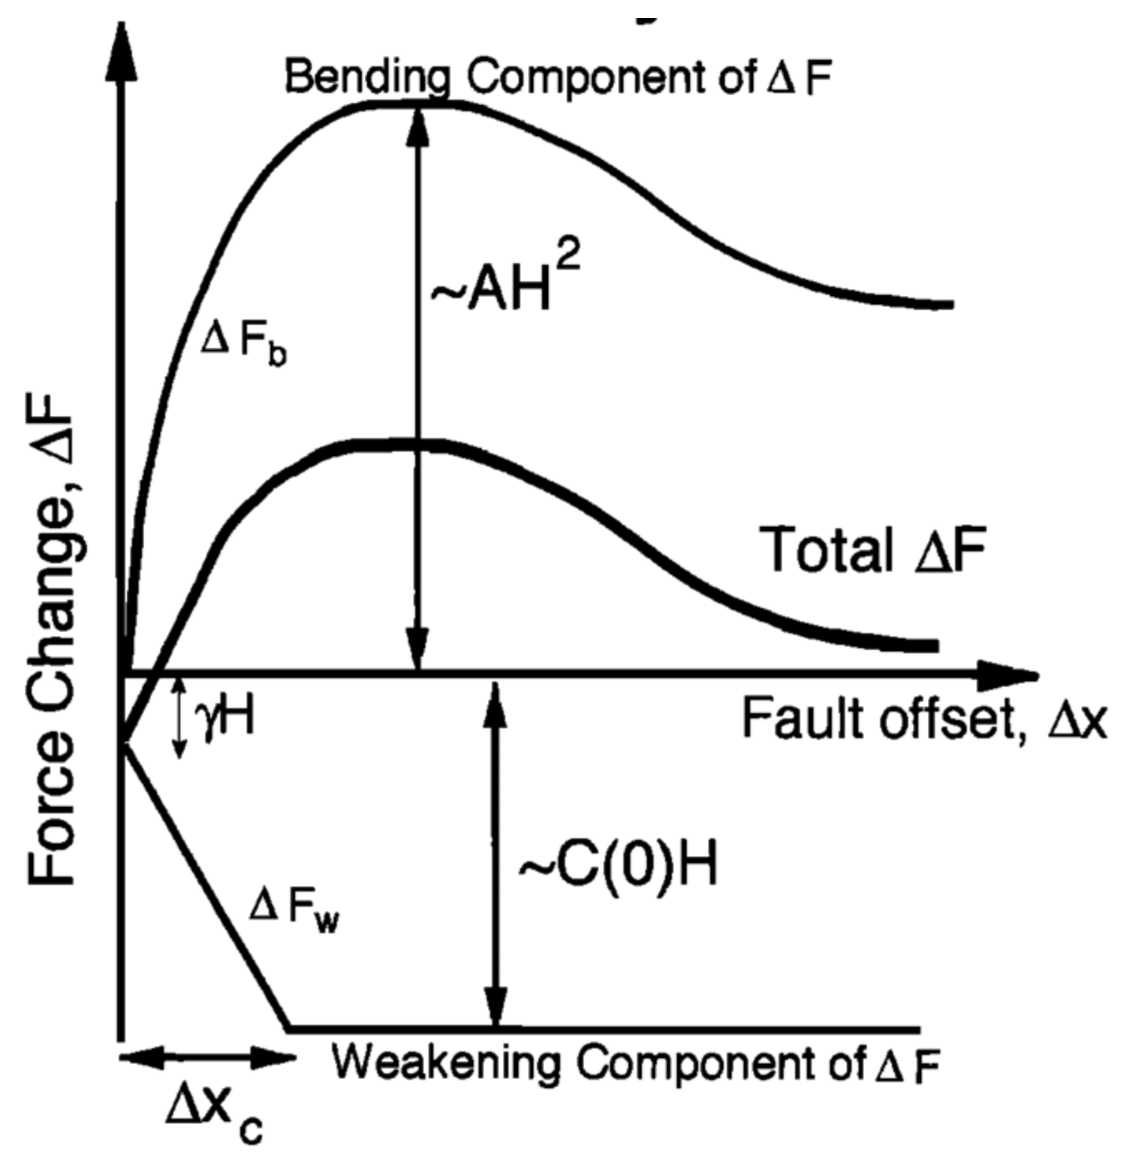
\includegraphics[width=0.45\textwidth]{./Figures/fig_Results_Weakening_1_tradeOff_bend_weak.eps}
 \caption[Trade-off between change in bending force $\Delta F_{b}$ and weakening in the fault interface $\Delta F_{w}$. Adapted from \citep{Lavier2000}.]{Trade-off between change in bending force $\Delta F_{b}$ and weakening in the fault interface $\Delta F_{w}$. H is the thickness of the brittle crust and $\gamma$ is the size of initial weak perturbation and A defines the maximum bending force change. Adapted from \citep{Lavier2000}. (For more details, please refer to \citep{Lavier2000})}
 \label{fig_Results_Weakening_1}
\end{figure}

\begin{figure}[h]
\noindent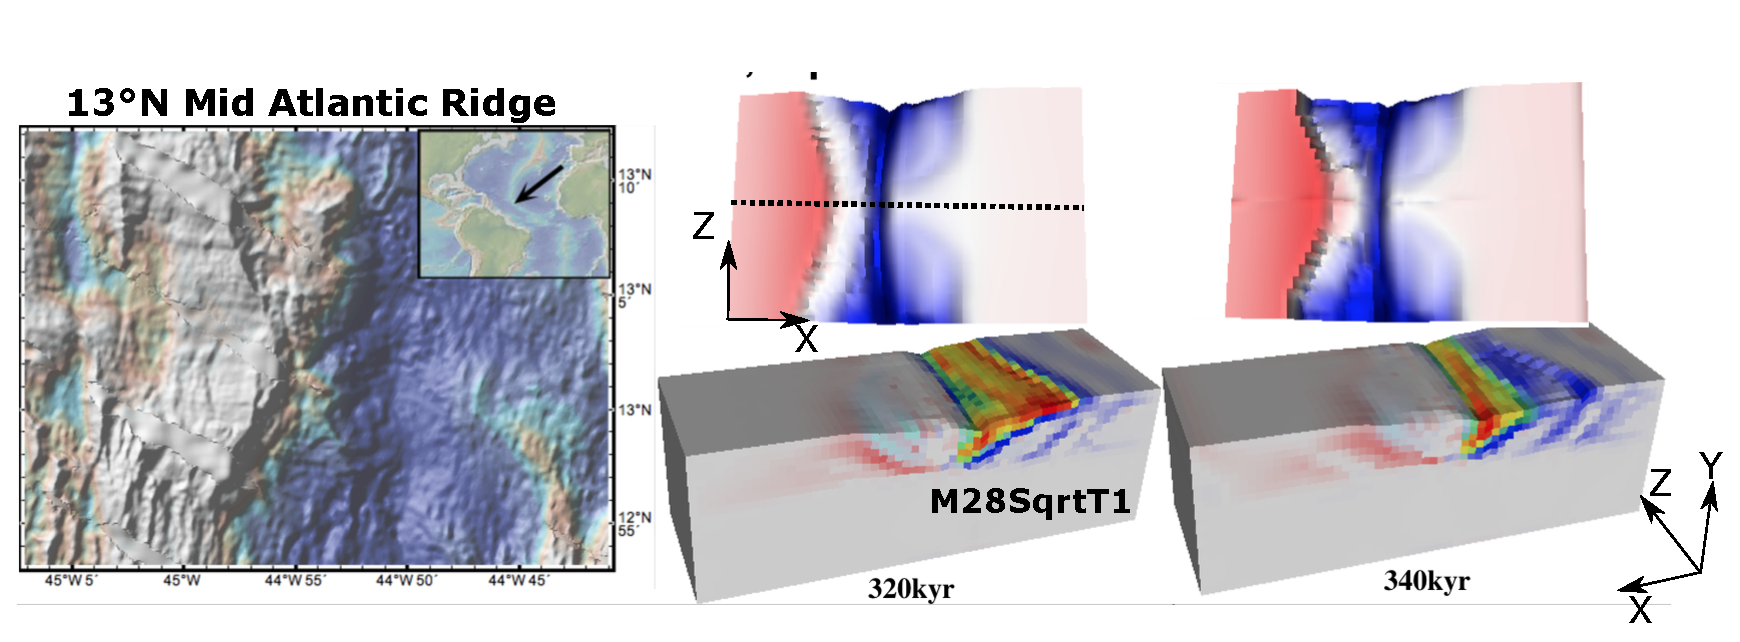
\includegraphics[width=1.0\textwidth]{./Figures/fig_Discussion_Observation_1_13N_MAR_CutBack.eps}
 \caption[Comparing bathymetry at 13$\degree$N Mid-Atlantic Ridge to the mass wasting behavior of M28SqrtT1.]{Comparing bathymetry at 13$\degree$N Mid-Atlantic Ridge to the mass wasting behavior of M28SqrtT1. The model topography is a mirror symetric flip according to the dash line, it shows the case of M varies in a square root functional form from 0.2 to 0.8 to 0.2. The bathymetry image is generated by GeoMapApp \citep{Ryan2009}.}
 \label{fig_Discussion_Observation_1_13N_MAR_CutBack}
\end{figure}

\begin{figure}[h]
\noindent\includegraphics[width=0.8\textwidth]{./Figures/fig_Discussion_Observation_3_MassWasting_13-15N_bathymetry_magnetizaion.eps}
 \caption[Bathymetry and magnetization of 13$\sim$15 $\degree$N MAR.]{Bathymetry and magnetization of 13$\sim$15 $\degree$N MAR. Bold lines are ridge axes. Lined up circles are identified isochrons. Adapted from \citep{Smith2008}.}
 \label{fig_Discussion_Observation_3_MassWasting_13-15N_bathymetry_magnetizaion}
\end{figure}

\begin{figure}[h]
\noindent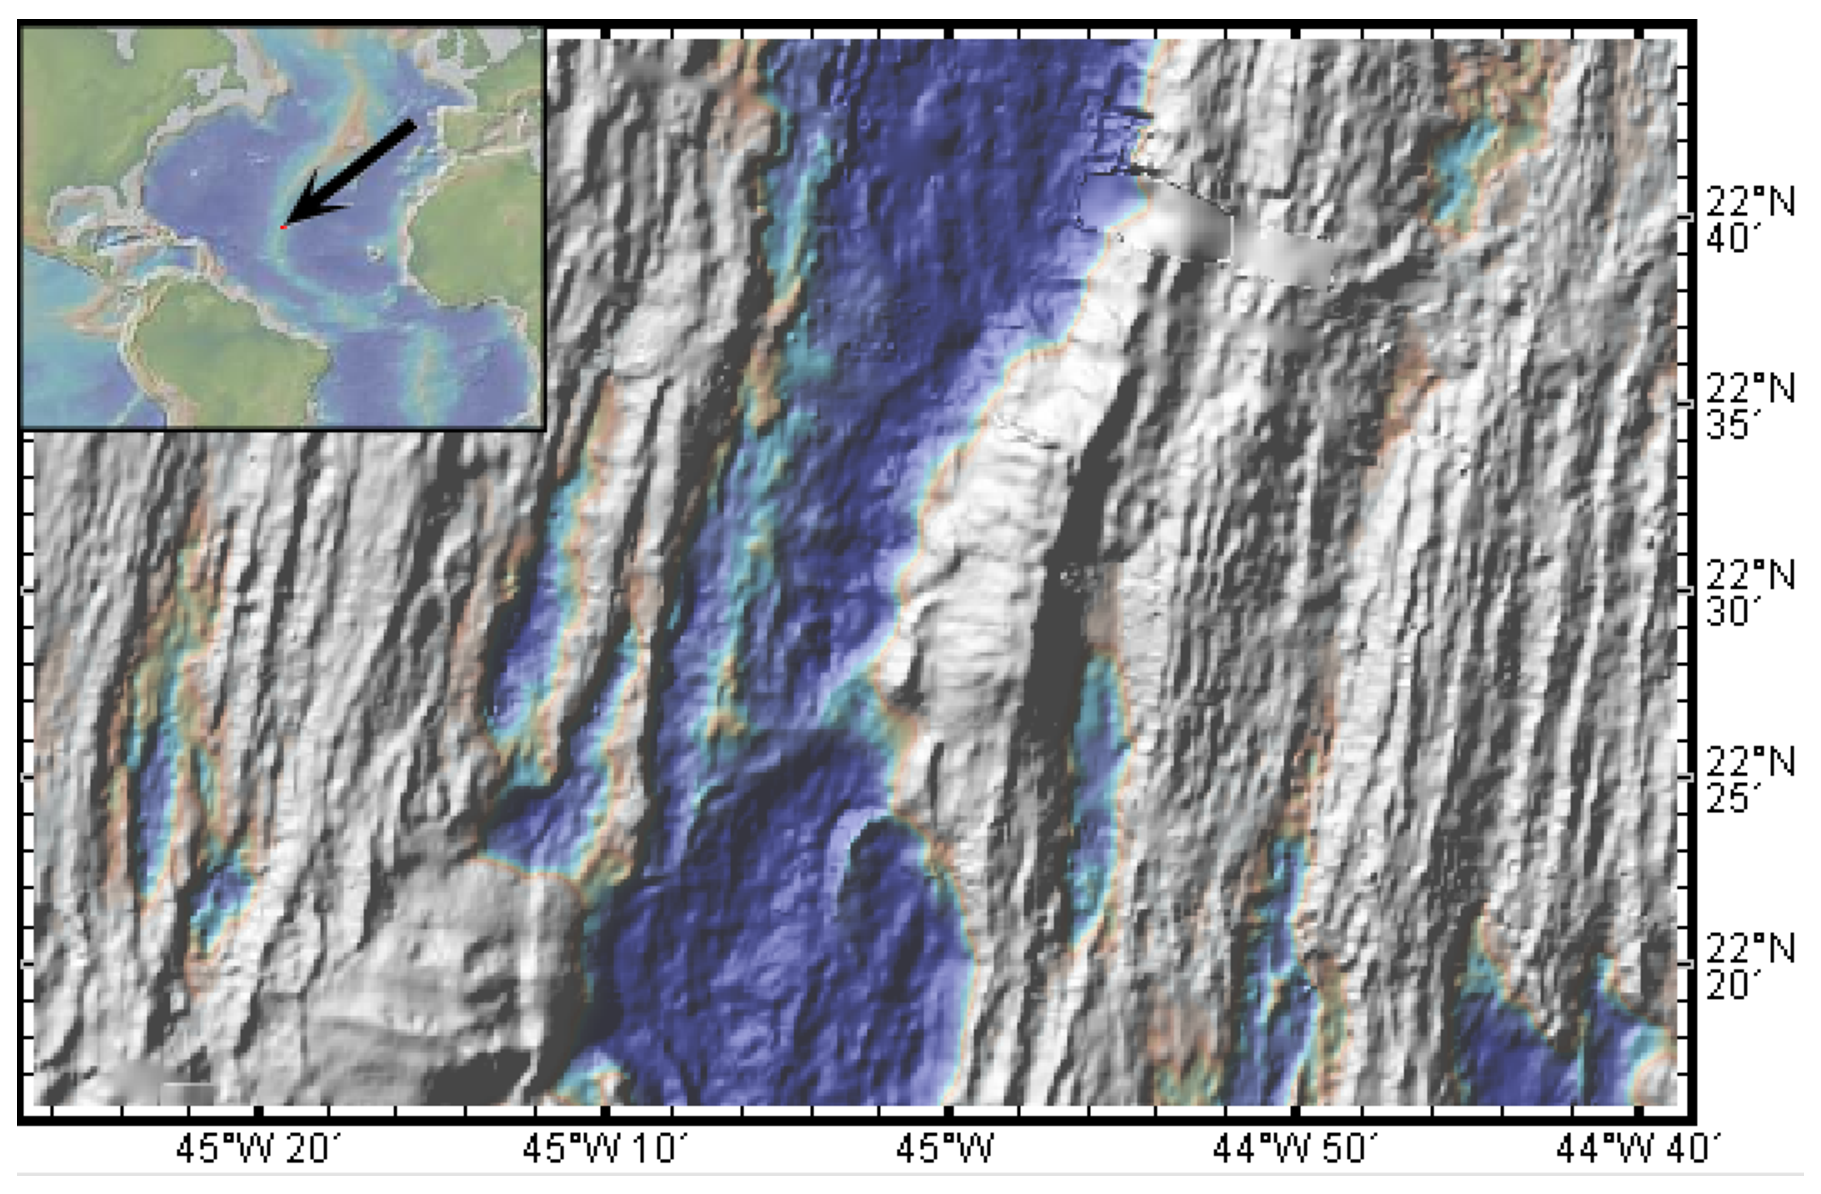
\includegraphics[width=0.5\textwidth]{./Figures/fig_Discussion_Observation_4_hourglass_22N_MAR.eps}
  \caption[Hourglass median valley at 22 $\degree$ 30 $^{\prime}$N MAR.]{Hourglass median valley at 22 $\degree$ 30 $^{\prime}$N MAR. Image is generated from GeoMapApp.}
 \label{fig_Discussion_Observation_4_hourglass_22N_MAR}
\end{figure}   

\begin{figure}[h]
\noindent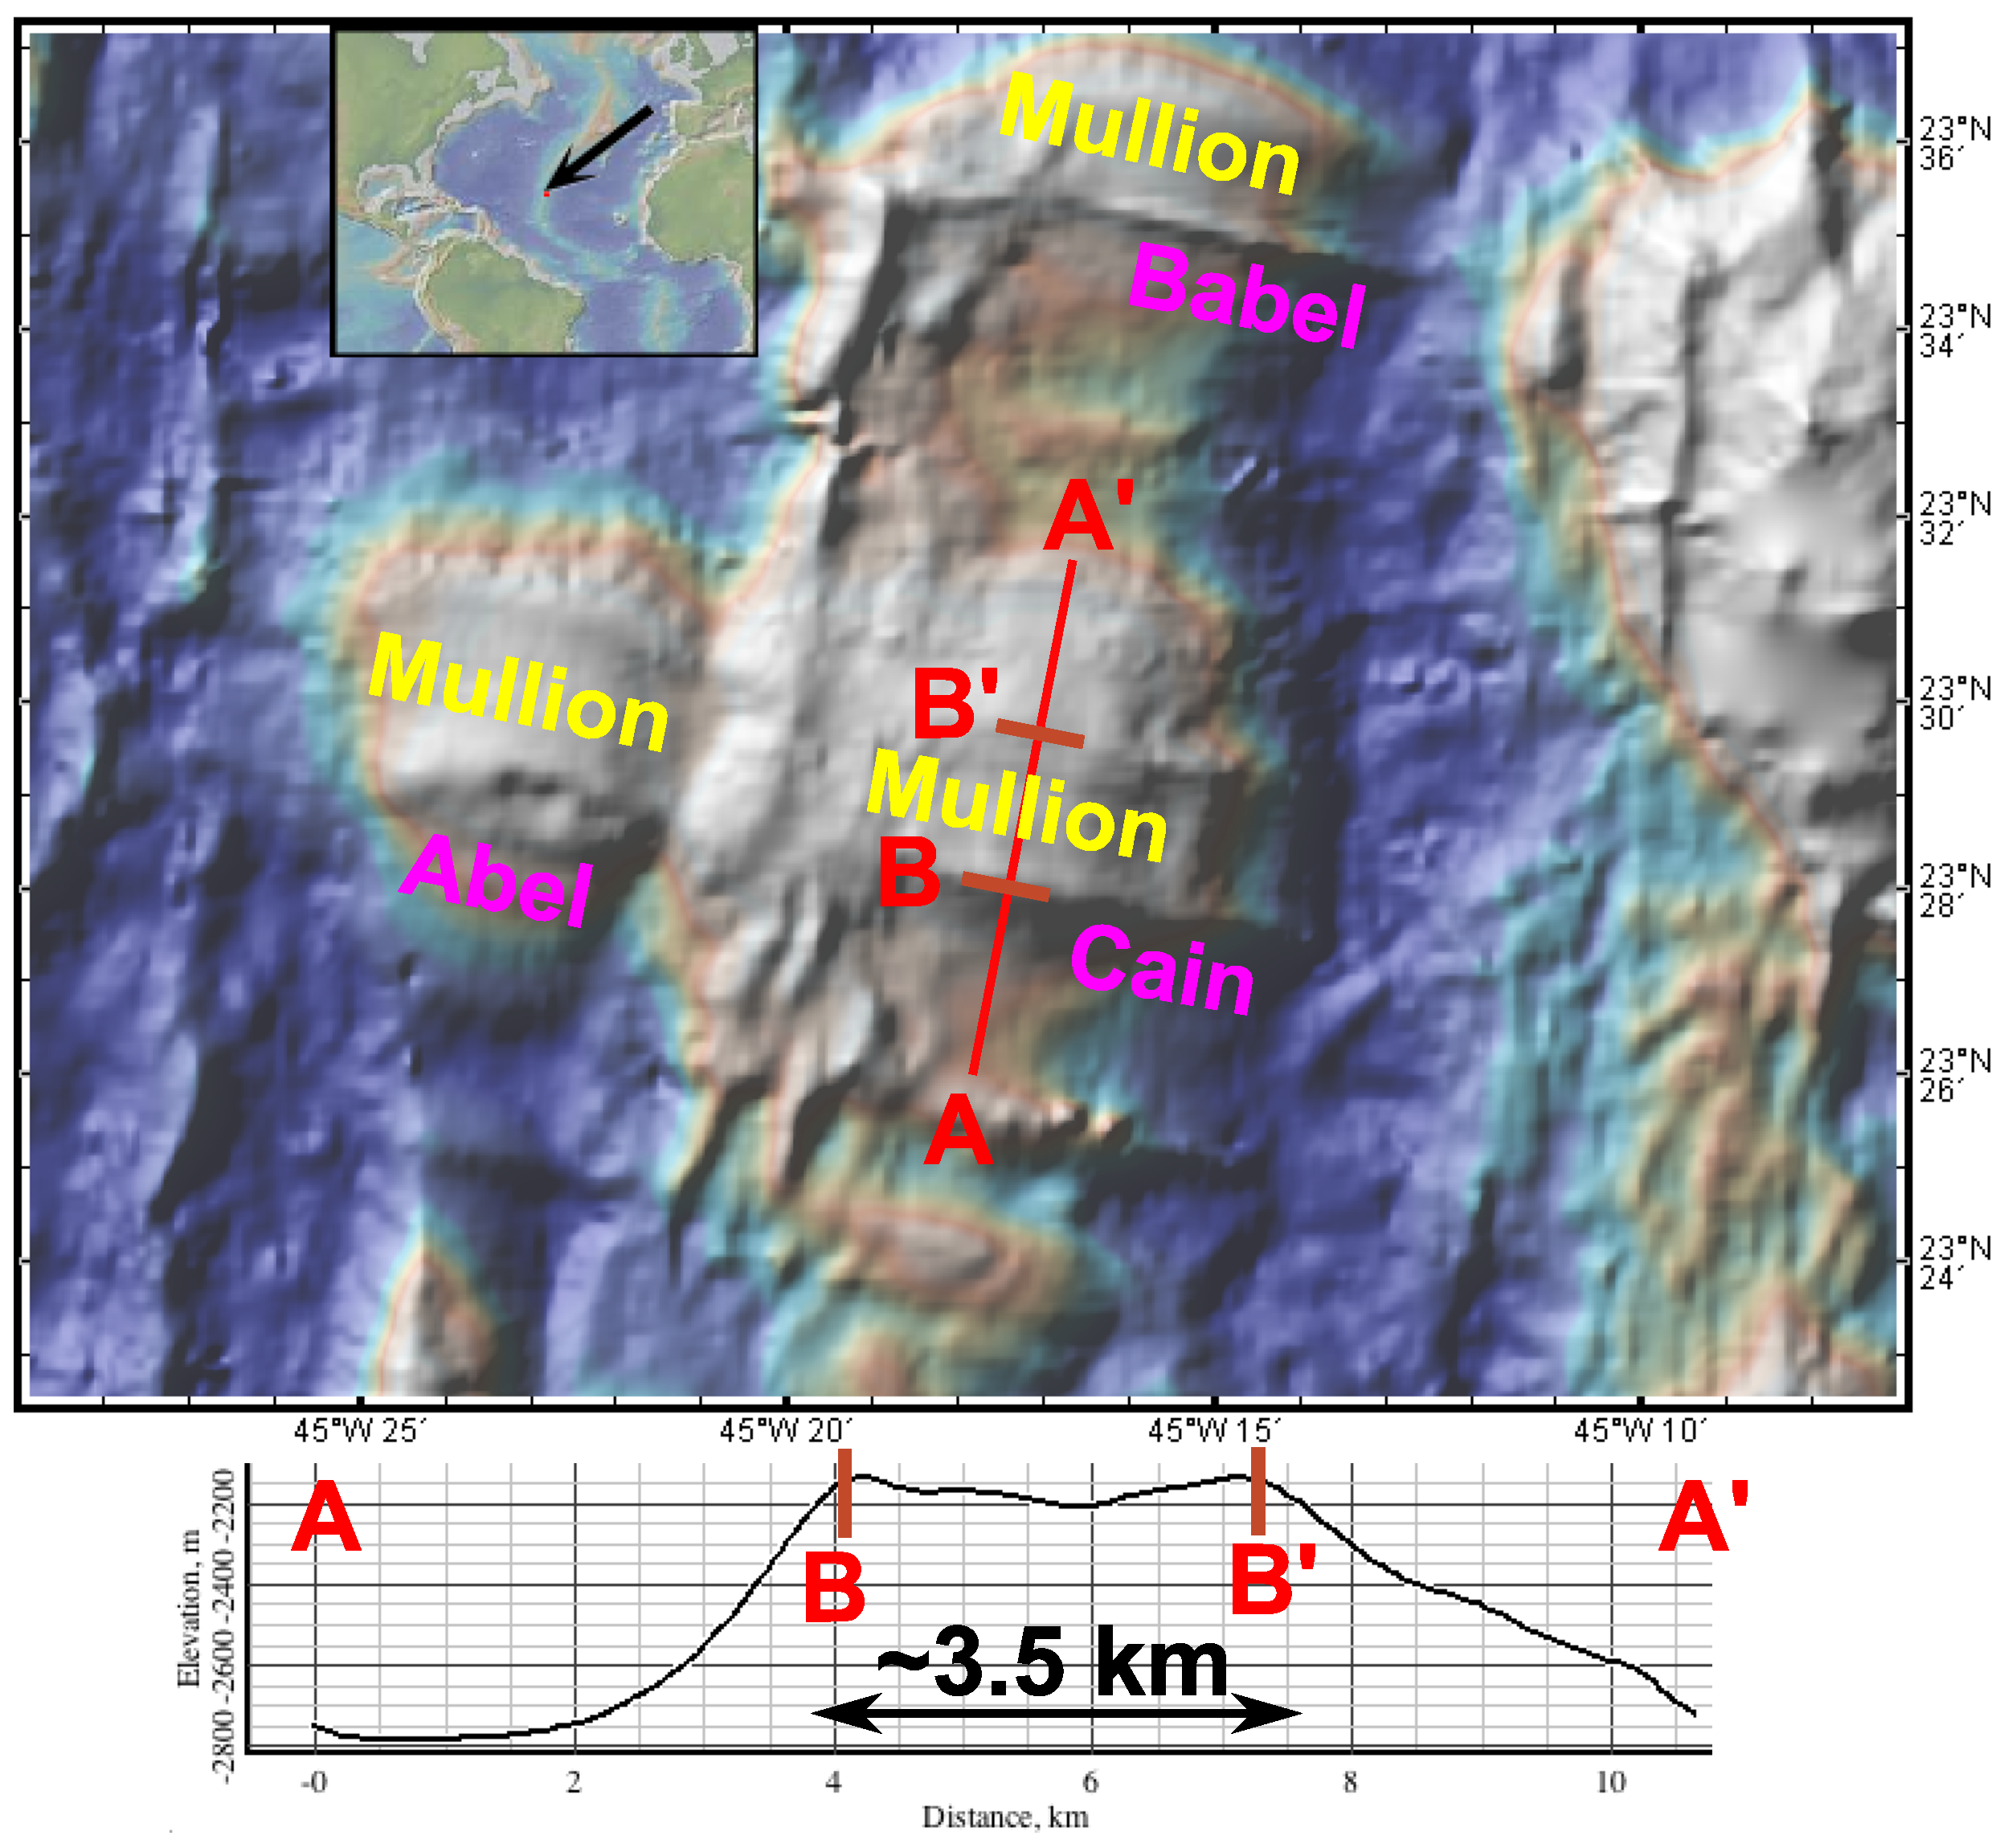
\includegraphics[width=0.8\textwidth]{./Figures/fig_Discussion_Observation_5_Mullion_Kane.eps}
  \caption[Bathymetry around the Kane OCC at 23 $\degree$N MAR.]{Bathymetry around the Kane OCC at 23 $\degree$N MAR. Image is generated from GeoMapApp.}
 \label{fig_Discussion_Observation_5_Mullion_Kane}
\end{figure}   

\begin{figure}[h]
\noindent\includegraphics[width=0.8\textwidth]{./Figures/TOBE_USED_fig_Discussion_Observation_Corrugations_16N_MAR.eps}
  \caption{Comparing bathymetry at 16 $\degree$N Mid-Atlantic Ridge to the corrugations of M58SinT1 at 550 kyr.}
 \label{fig_Discussion_Observation_Corrugations16N_M58SinT1}
\end{figure}

\begin{figure}[h]
\noindent\includegraphics[width=0.5\textwidth]{./Figures/fig_Discussion_simple_models_for_corrugation_mechanism.eps}
  \caption[Simpler 3D models for formation mechanism of corrugation.]{a) Plastic strain evolution of simpler 3D model with 4 km of seawater pressure on top; b) Plastic strain evolution of simpler 3D model with 10 km of seawater pressure on top. Seeds (elements with initial plastic strain) are partially added along the ridge segment.}
 \label{fig_Discussion_simple_models_for_corrugation_mechanism}
\end{figure}

\begin{figure}[h]
\noindent\includegraphics[width=0.5\textwidth]{./Figures/fig_Discussion_Observation_6_Corrugation_simplerModel_4kwaterdepth_along_ridge_seed.eps}
  \caption[Simpler 3D model with 4 km of seawater pressure on top. Seeds are added along the whole ridge segment.]{Simpler 3D model with 4 km of seawater pressure on top. Seeds are added along the whole ridge segment. Color scale is the same as Figure~\ref{fig_Results_3_2_6_corrugations_evolution}.}
 \label{fig_Discussion_Observation_6_Corrugation_simplerModel_4kwaterdepth_along_ridge_seed}
\end{figure}   

%<>1



\end{document}

%%%%%%%%%%%%%%%%%%%%%%%%%%%%%%%%%%%%%%%%%%%%%%%%%%%%%%%%%%%%%%%

More Information and Advice:

%% ------------------------------------------------------------------------ %%
%
%  SECTION HEADS
%
%% ------------------------------------------------------------------------ %%

% Capitalize the first letter of each word (except for
% prepositions, conjunctions, and articles that are
% three or fewer letters).

% AGU follows standard outline style; therefore, there cannot be a section 1 without
% a section 2, or a section 2.3.1 without a section 2.3.2.
% Please make sure your section numbers are balanced.
% ---------------
% Level 1 head
%
% Use the \section{} command to identify level 1 heads;
% type the appropriate head wording between the curly
% brackets, as shown below.
%
%An example:
%\section{Level 1 Head: Introduction}
%
% ---------------
% Level 2 head
%
% Use the \subsection{} command to identify level 2 heads.
%An example:
%\subsection{Level 2 Head}
%
% ---------------
% Level 3 head
%
% Use the \subsubsection{} command to identify level 3 heads
%An example:
%\subsubsection{Level 3 Head}
%
%---------------
% Level 4 head
%
% Use the \subsubsubsection{} command to identify level 3 heads
% An example:
%\subsubsubsection{Level 4 Head} An example.
%
%% ------------------------------------------------------------------------ %%
%
%  IN-TEXT LISTS
%
%% ------------------------------------------------------------------------ %%
%
% Do not use bulleted lists; enumerated lists are okay.
% \begin{enumerate}
% \item
% \item
% \item
% \end{enumerate}
%
%% ------------------------------------------------------------------------ %%
%
%  EQUATIONS
%
%% ------------------------------------------------------------------------ %%

% Single-line equations are centered.
% Equation arrays will appear left-aligned.

Math coded inside display math mode \[ ...\]
 will not be numbered, e.g.,:
 \[ x^2=y^2 + z^2\]

 Math coded inside \begin{equation} and \end{equation} will
 be automatically numbered, e.g.,:
 \begin{equation}
 x^2=y^2 + z^2
 \end{equation}

% IF YOU HAVE MULTI-LINE EQUATIONS, PLEASE
% BREAK THE EQUATIONS INTO TWO OR MORE LINES
% OF SINGLE COLUMN WIDTH (20 pc, 8.3 cm)
% using double backslashes (\\).

% To create multiline equations, use the
% \begin{eqnarray} and \end{eqnarray} environment
% as demonstrated below.
\begin{eqnarray}
  x_{1} & = & (x - x_{0}) \cos \Theta \nonumber \\
        && + (y - y_{0}) \sin \Theta  \nonumber \\
  y_{1} & = & -(x - x_{0}) \sin \Theta \nonumber \\
        && + (y - y_{0}) \cos \Theta.
\end{eqnarray}

%If you don't want an equation number, use the star form:
%\begin{eqnarray*}...\end{eqnarray*}

% Break each line at a sign of operation
% (+, -, etc.) if possible, with the sign of operation
% on the new line.

% Indent second and subsequent lines to align with
% the first character following the equal sign on the
% first line.

% Use an \hspace{} command to insert horizontal space
% into your equation if necessary. Place an appropriate
% unit of measure between the curly braces, e.g.
% \hspace{1in}; you may have to experiment to achieve
% the correct amount of space.


%% ------------------------------------------------------------------------ %%
%
%  EQUATION NUMBERING: COUNTER
%
%% ------------------------------------------------------------------------ %%

% You may change equation numbering by resetting
% the equation counter or by explicitly numbering
% an equation.

% To explicitly number an equation, type \eqnum{}
% (with the desired number between the brackets)
% after the \begin{equation} or \begin{eqnarray}
% command.  The \eqnum{} command will affect only
% the equation it appears with; LaTeX will number
% any equations appearing later in the manuscript
% according to the equation counter.
%

% If you have a multiline equation that needs only
% one equation number, use a \nonumber command in
% front of the double backslashes (\\) as shown in
% the multiline equation above.

%% ------------------------------------------------------------------------ %%
%
%  SIDEWAYS FIGURE AND TABLE EXAMPLES
%
%% ------------------------------------------------------------------------ %%
%
% For tables and figures, add \usepackage{rotating} to the paper and add the rotating.sty file to the folder.
% AGU prefers the use of {sidewaystable} over {landscapetable} as it causes fewer problems.
%
% \begin{sidewaysfigure}
% \includegraphics[width=20pc]{samplefigure.eps}
% \caption{caption here}
% \label{label_here}
% \end{sidewaysfigure}
%
%
%
% \begin{sidewaystable}
% \caption{}
% \begin{tabular}
% Table layout here.
% \end{tabular}
% \end{sidewaystable}
%
%

